% ******************************* PhD Thesis Template **************************
% Please have a look at the README.md file for info on how to use the template

% **************************** Formatting & Metadata ***************************

\documentclass[a4paper,12pt,print]{input_files/cls/thesis}
%\documentclass[a4paper,12pt,print]{input_files/cls/thesis2}
% See README.md for option details

% ******************************************************************************
% ****************************** Custom Margin *********************************

% Add spaces between paragraphs
\setlength{\parskip}{0.5em}
% Ragged bottom avoids extra whitespaces between paragraphs
\raggedbottom
% To remove the excess top spacing for enumeration, list and description
%\usepackage{enumitem}
%\setlist[enumerate,itemize,description]{topsep=0em}

% *****************************************************************************
% ******************* Fonts (like different typewriter fonts etc.)*************

% Add `customfont' in the document class option to use this section

% *****************************************************************************
% **************************** Custom Packages ********************************
% *****************************************************************************
% NB: Packages (without options) loaded in thesis class:
%  lscape, setspace, calc, ifthen, ifpdf, ifxetex, epstopdf, datetime,
%  everypage, textcomp, mathptmx, fourier, lmodern, amsmath, fontspec,
%  unicode-math, amsfonts, amssymb, url, breakurl, fancyhdr,
% NB: Packages (with [options]) loaded in thesis class:
%  tocbibind[nottoc], appendix[title,titletoc], color[usenames, dvipsnames],
%  lineno[switch,pagewise,mathlines], textpos[absolute], graphicx[pdftex,demo],
%  biblatex[various options depending on other settings],
%  natbib[various options depending on other settings],
%  geometry[various options depending on other settings],
%  inputenc[utf8], fontenc[T1], microtype[final],
%  hyperref[unicode=true, hidelinks], nomencl[intoc],
%\usepackage{fancyvrb}
%\usepackage{framed}
\usepackage{subcaption}
\usepackage{wrapfig}
\usepackage{setspace}
\usepackage{todonotes}
\usepackage{tcolorbox}
\usepackage{threeparttable}
\usepackage{booktabs}
\usepackage{xstring}
\usepackage{mfirstuc}
\usepackage{xspace}
\usepackage{afterpage}
\usepackage{placeins}
\usepackage{array}
\usepackage[docdef=true,nonumberlist]{glossaries-extra}
\usepackage{textgreek}
\usepackage{makeidx}
%\usepackage{subfiles}
% ************************* Algorithms and Pseudocode **************************

%\usepackage{algpseudocode}


% ********************Captions and Hyperreferencing / URL **********************

% Captions: This makes captions of figures use a boldfaced small font.
%\RequirePackage[small,bf]{caption}

\RequirePackage[labelsep=colon,tableposition=top,labelfont=bf,font=small]{caption}
\renewcommand{\figurename}{Figure} %to support older versions of captions.sty


% *************************** Graphics and figures *****************************
\hyphenation{circRNA}
\hyphenation{circRNAs}

%\usepackage{rotating}

% Uncomment the following two lines to force Latex to place the figure.
% Use [H] when including graphics. Note 'H' instead of 'h'
%\usepackage{float}
%\restylefloat{figure}

% Subcaption package is also available in the sty folder you can use that by
% uncommenting the following line
% This is for people stuck with older versions of texlive
%\usepackage{sty/caption/subcaption}
\usepackage{subcaption}

% ********************************** Tables ************************************
\usepackage{booktabs} % For professional looking tables
\usepackage{multirow}

%\usepackage{multicol}
%\usepackage{longtable}
%\usepackage{tabularx}


% *********************************** SI Units *********************************
\usepackage{siunitx} % use this package module for SI units


% ******************************* Line Spacing *********************************

% Choose linespacing as appropriate. Default is one-half line spacing as per the
% University guidelines

% \doublespacing
% \onehalfspacing
% \singlespacing


% ************************ Formatting / Footnote *******************************
\usepackage{listings}

% Don't break enumeration (etc.) across pages in an ugly manner (default 10000)
%\clubpenalty=500
%\widowpenalty=500

%\usepackage[perpage]{footmisc} %Range of footnote options


% *****************************************************************************
% *************************** Bibliography  and References ********************

\usepackage{cleveref} %Referencing without need to explicitly state fig /table
\RequirePackage[backend=biber, citestyle=numeric-comp, style=nature, intitle=true, sorting=none, natbib=true, maxnames=3, minnames=1, url=false, giveninits=true, sortcites=true, date=year, doi=false,isbn=false]{biblatex}

\bibliography{input_files/References.bib}

% ******************************************************************************
% ************************* User Defined Commands ******************************
% ******************************************************************************

% *********** To change the name of Table of Contents / LOF and LOT ************

%\renewcommand{\contentsname}{My Table of Contents}
%\renewcommand{\listfigurename}{My List of Figures}
%\renewcommand{\listtablename}{My List of Tables}

\usepackage{calc}
\makeatletter
\newcommand{\tocfill}{\cleaders\hbox{$\m@th \mkern\@dotsep mu . \mkern\@dotsep mu$}\hfill}
\makeatother
\newcommand{\abbrlabel}[1]{\makebox[8cm][l]{#1\ \tocfill}}
\newenvironment{abbreviations}{\begin{list}{}{\renewcommand{\makelabel}{\abbrlabel}%
        \setlength{\labelwidth}{8cm}\setlength{\leftmargin}{\labelwidth+\labelsep}%
                                              \setlength{\itemsep}{0pt}}}{\end{list}}

% ********************** TOC depth and numbering depth *************************

\setcounter{secnumdepth}{3}
\setcounter{tocdepth}{2}


% ******************************** Units **********************************

%% CUSTOM UNIT COMMAND %%
\newcommand{\cu}[2]{\SI[detect-weight]{#2}{#1}} % custom unit

%% TIME %%
\newcommand{\secs}{\cu{\second}} % Seconds
\newcommand{\mins}{\cu{\minute}} % Minutes
\newcommand{\hr}{\cu{\hour}} % Hours

%% VOLUME %%
\DeclareSIUnit\vols{vol} % volumes (relative to some reference)
\newcommand{\vol}{\cu{\vols}} % volumes
\newcommand{\ml}{\cu{\milli\litre}} % millilitres
\newcommand{\ul}{\cu{\micro\litre}} % microlitres
\newcommand{\lt}{\cu{\liter}} % litres

%% MASS %%
\let\ng\undefined
\newcommand{\ng}{\cu{\nano\gram}} % nanograms
\newcommand{\ug}{\cu{\micro\gram}} % micrograms
\newcommand{\mg}{\cu{\milli\gram}} % milligrams
\newcommand{\gr}{\cu{\gram}} % grams
\DeclareSIUnit\Unit{U} % enzyme units
\newcommand{\units}{\cu{\Unit}} % units of enzyme

%% CONCENTRATION %%
% Molar
\DeclareSIUnit\Molar{M} % Molar, = 1 mole per litre
\newcommand{\mol}{\cu{\Molar}} % molar
\newcommand{\mmol}{\cu{\milli\Molar}} % millimolar
\newcommand{\umol}{\cu{\micro\Molar}} % micromolar
\newcommand{\nmol}{\cu{\nano\Molar}} % nanomolar
% Mass per volume (e.g. for nucleic acids)
\newcommand{\ngul}{\cu{\nano\gram\per\micro\litre}} % ng/ul
\newcommand{\ngml}{\cu{\nano\gram\per\milli\litre}} % ng/ml
\newcommand{\ugml}{\cu{\micro\gram\per\milli\litre}} % ug/ml
\newcommand{\mgml}{\cu{\milli\gram\per\milli\litre}} % mg/ml
\newcommand{\gl}{\cu{\gram\per\liter}} % g/L
% Units per volume (for enzymes)
\newcommand{\unitsul}{\cu{\Unit\per\micro\litre}} % units/ul, for enzymes
% Percentages
\newcommand{\pc}{\cu{\percent}} % percent concentration (e.g. ethanol)
% Multiples
\DeclareSIUnit\X{\times} % x concentration, e.g. for buffers
\let\x\undefined
\newcommand{\x}{\cu{\X}}

%% TEMPERATURE %%
\newcommand{\degC}[1]{\SI[detect-weight]{#1}{\degreeCelsius}} % degrees celcius
\newcommand{\degrees}[1]{\SI[detect-weight]{#1}{\degree}}

%% PH %%
\DeclareSIUnit{\pH}{pH~}
\newcommand{\ph}[1]{\SI[detect-weight]{#1}[\pH]{}} % pH (as pre-unit)

%% CENTRIFUGE SPEED %%
\DeclareSIUnit{\G}{\mathit{g}} % x standard gravity
\DeclareSIUnit{\RPM}{rpm} % revolutions per minute
\newcommand{\g}[1]{\IfStrEq{#1}{top speed}{top speed}{\SI[detect-weight]{#1}{\G}}}
\newcommand{\rpm}{\cu{\RPM}}

%% BIOLOGICAL SEQUENCE LENGTH %%

\DeclareSIUnit{\B}{b} % Base (for kb etc)
\DeclareSIUnit{\BP}{bp} % Base pairs
\DeclareSIUnit{\NT}{nt} % Nucleotides
\newcommand{\bp}{\cu{\BP}}
\newcommand{\kb}{\cu{\kilo\B}}
\newcommand{\mb}{\cu{\mega\B}}
\newcommand{\nt}{\cu{\NT}}

%% LENGTH %%
\newcommand{\nm}{\cu{\nano\metre}}
\newcommand{\um}{\cu{\micro\metre}}
\newcommand{\mm}{\cu{\milli\metre}}


% ******************************** Autoref settings **********************************
%\renewcommand*{\sectionautorefname}{Section}
%\renewcommand*{\subsectionautorefname}{Section}
%\renewcommand*{\chapterautorefname}{Chapter}
%\newcommand*{\appendixautorefname}{Appendix}
%\newcommand*{\Appendixautorefname}{Appendix}

% ******************************** Misc. commands **********************************

\newcommand{\cm}[1]{C$_\mu$#1}
\newcommand{\cd}[1]{C$_\delta$#1}
\newcommand{\cz}[1]{C$_\zeta$#1}

\newcommand{\question}[1]{\subsection{#1}}
%\newcommand{\question}[1]{\textit{\Large #1}\\}
\newcommand{\q}[1]{\question{#1}}

\renewcommand\thesubfigure{\Alph{subfigure}}
\renewcommand\thesubtable{\Alph{subtable}}

\definecolor{codegreen}{rgb}{0,0.6,0}
\definecolor{codegray}{rgb}{0.5,0.5,0.5}
\definecolor{codepurple}{rgb}{0.58,0,0.82}
\definecolor{backcolour}{rgb}{0.95,0.95,0.92}

\lstset{
    backgroundcolor=\color{backcolour},   
    commentstyle=\color{codegreen},
	basicstyle=\ttfamily,
	columns=fixed,
	%frame=single,
    breaklines=true,
    breakatwhitespace=true,
    postbreak=\mbox{\textcolor{red}{$\hookrightarrow$}\space},
    language=bash,
    keepspaces=true,
    showstringspaces=false,
    aboveskip=0.3em,
    belowskip=0.3em,
    upquote=true,
    }

% Quick formatting commands
\newcommand{\gene}[1]{\textit{#1}}
\newcommand{\igh}[1]{\gene{IGH{#1}}}

% Species names (with and without genus abbreviation)
\newcommand{\species}[2]{\textit{\capitalisewords{#1} #2}\xspace}
\newcommand{\nfu}{\species{Nothobranchius}{furzeri}}
\newcommand{\Nfu}{\species{N.}{furzeri}}
\newcommand{\xma}{\species{Xiphophorus}{maculatus}}
\newcommand{\Xma}{\species{X.}{maculatus}}


% Program/package names and code snippets
\newcommand{\program}[1]{#1}
%\newcommand{\program}[2][bash]{\lstinline[language=#1]{#2}} %[]
\newcommand{\snippet}[2][bash]{\lstinline[language=#1]{#2}} %[]

% IGH locus components
\let\dh\undefined
\newcommand{\vh}{VH\xspace}
\newcommand{\dh}{DH\xspace}
\newcommand{\jh}{JH\xspace}
\newcommand{\ch}{CH\xspace}

% File formats
%\newcommand{\fmt}[1]{\texttt{\MakeUppercase{#1}}}
\newcommand{\fmt}[1]{\MakeUppercase{#1}}
\newcommand{\format}[1]{\fmt{#1}}

% Sequence
\newcommand{\sequence}[1]{\texttt{\MakeUppercase{#1}}}

% Ig-Seq
\newcommand{\igseq}{IgSeq\xspace}
\newcommand{\Igseq}{immunoglobulin sequencing\xspace}
\newcommand{\IGSEQ}{Immunoglobulin sequencing\xspace}
\newcommand{\naive}{na\"{i}ve\xspace}
\newcommand{\Naive}{Na\"{i}ve\xspace}


%% Start of subappendices environment
%\AtBeginEnvironment{subappendices}{%
%\chapter*{Appendices}
%\addcontentsline{toc}{chapter}{Appendices}
%\counterwithin{figure}{section}
%\counterwithin{table}{section}
%}
%
%% End of subappendices environment
%\AtEndEnvironment{subappendices}{%
%\counterwithout{figure}{section}
%\counterwithout{table}{section}
%}

\makeatletter
\newcommand\notsotiny{\@setfontsize\notsotiny\@viipt\@viiipt}
\newcommand\evenlesstiny{\@setfontsize\notsotiny\@viiipt\@ixpt}
\makeatother

\newcommand{\subsubsubsection}[1]{\noindent\textit{#1}\noindent}

\newcommand{\etc}{\textit{et cetera}\xspace}

\renewcommand{\floatpagefraction}{.85}%
\renewcommand{\topfraction}{.85}%
\renewcommand{\bottomfraction}{.50}%

% Embed text values in thesis
\newcommand{\embed}[1]{\input{#1}\unskip}

\newcommand{\Caption}[2]{\caption[#1]{\textbf{#1:} #2}}


% Generate glossary
\makeglossaries
 %Contains packages and user-defined commands and settings
%
%% ************************ Thesis Information & Meta-data **********************
%
% ************************ Thesis Information & Meta-data **********************
%% The title of the thesis
\title{Characterising antibody immunity and ageing in a short-lived teleost}

%% Subtitle (Optional)
%\subtitle{}
%\submissiontext

%% The full name of the author
\author{William John Bradshaw}

%% Department (eg. Department of Engineering, Maths, Physics)
\dept{aus Hastings} %! Really?

%% University and Crest
%\university{University of Cologne, Germany}
% Crest minimum should be 30mm.
\crest{
\includegraphics[width=0.5\textwidth]{_Meta/Logos/UoC_Crest}}

%% Use this crest, if you are using the college crest
%% Crest long miminum should be 65mm
%\crest{\includegraphics[width=0.45\textwidth]{University_Crest_Long}}

%% College shield [optional] 
% Crest minimum should be 30mm.
%\collegeshield{\includegraphics[width=0.2\textwidth]{CollegeShields/Kings}}


% Supervisor (optional)
% for multiple supervisors, append each supervisor with the \newline command
\supervisor{Dr. Dario Riccardo Valenzano\newline Prof. Dr. Andreas Beyer}

%% Supervisor line width: required to align supervisors
\supervisorlinewidth{\textwidth}


%% You can redefine the submission text:
% Default as per the University guidelines:
% ``This dissertation is submitted for the degree of''
%\renewcommand{\submissiontext}{change the default text here if needed}

%% Full title of the Degree
%\degreetitle{Doctor of Philosophy}

%% College affiliation (optional)
%\college{MPI for Biology of Ageing}

%% Submission date
% Default is set as {\monthname[\the\month]\space\the\year}
%\degreedate{September 2014} 

%%% Meta information
%\subject{LaTeX} \keywords{{LaTeX} {PhD Thesis} {Engineering} {University of
%Cambridge}}
 % Thesis title and author information, other metadata

% ***************************** Chapter Mode ***********************************
% The chapter mode allows user to only print particular chapters with references
% Title, Contents, Frontmatter are disabled by default
% Useful option to review a particular chapter or to send it to supervisior.
% To use choose `chapter' option in the document class

\ifdefineChapter
\chapter{Introduction}
\label{chap:intro}
\onehalfspacing

\pagebreak

\section{Overview}
\label{sec:intro_overview}

All organisms exist in a state of intense competition for resources. For many organisms, among the most dangerous competitors are parasites, which attempt to colonise the host's own body and co-opt its internal resources and systems to their own advantage. The evolutionary arms race between parasites and hosts is ancient, and has led to the development of a stunning variety of complex offensive and defensive adaptations on each side \parencite{jack2015evolution}. Immunology has therefore had a profound effect on evolution.

One of the most complex and sophisticated systems developed as part of this ancient host/parasite conflict is the vertebrate adaptive immune system. By dynamically recombining their own DNA within specialised lymphocyte cells (\Cref{sec:intro_immunity_primary}), jawed vertebrates are capable of producing an almost unlimited variety of different \textit{de novo} antigen-receptor proteins, and hence of responding effectively to entirely novel immune threats \parencite{jack2015evolution}. In addition, by producing long-lived memory cells in response to antigenic stimulation, the adaptive immune system can retain the ability to respond to recurrent threats years or even decades after they were first encountered by an individual \parencite{kurosaki2015memory} (\Cref{sec:intro_affinity_maturation}). This combination of dynamic adaptability to novel immune threats and persistent immune memory enables vertebrates to progressively improve their protection against predictable aspects of their immune environment \parencite{mayer2018memory}, while also coping effectively with the rapid evolution of bacterial and viral pathogens.

Among the different branches of vertebrate adaptive immunity, the B-cell-mediated humoral immune system is unique in both the breadth of antigenic compounds it can respond to and its ability to produce secreted antigen-receptor proteins capable of acting independently of the cells that produced them. Whereas the T-lymphocytes of the cellular adaptive immune system can respond only to processed peptide antigens expressed on the surface of antigen-presenting cells, the antibodies produced by B-lymphocytes (\Cref{sec:intro_antibody_structure}) are capable of responding to a much wider variety of organic molecules, including proteins, carbohydrates, nucleic acids, and lipids \parencite{sompayrac2019immune}. Secreted antibodies in serum and mucosal secretions play a number of essential roles in vertebrate immunity, including opsonisation (recruitment of phagocytic cells), activation of complement, and inactivation and aggregation of antigens and pathogens \parencite{schroeder2010immunoglobulins}, while membrane-bound antibodies (also known as B-cell receptors or BCRs \parencite{bengten2015fishantibodies}) orchestrate B-cell development and response to antigen exposure. An effective humoral immune system is essential to immune function in vertebrates, and mutations that impair antibody production can cause severe immunodeficiency syndromes in humans \parencite{vanzelm2006cd19}.

Despite all its sophistication, however, the functionality of the vertebrate adaptive immune system declines dramatically with age, leaving older individuals increasingly vulnerable to infectious disease (\Cref{sec:intro_immunosenescence}). In humans and other species, the decline in immune functionality with age manifests as a dramatic increase in deaths from infection in older people, as well as increasing levels of infection-associated morbidity and a decline in the effectiveness of pro-immune interventions such as vaccination \parencite{sambhara2009vaccination}. The molecular and physiological changes underlying this immunosenescent phenotype are wide-ranging, implicating many different parts of the immune system; however, one particularly important contributor is the systemic decline in the effectiveness of the adaptive immune system. For the humoral immune system, well-established immunosenescent phenotypes include a fall in \naive B-cell output from the bone marrow, reduced antibody quality, impaired affinity maturation, and a serious decline in the ability to mount an effective antibody response to vaccination (\Cref{sec:intro_immunosenescence}).

While much has been discovered about the cellular and physiological changes that take place in the humoral adaptive immune system with age in some species, particularly humans and mice, much less is known about how these changes translate to alterations in the high-level diversity, clonal makeup, and other structural aspects of the overall antibody repertoire in older individuals. Such a high-level systemic approach to antibody diversity could potentially reveal a great deal about how ageing and other processes affect adaptive immune functionality in an organism. Specialised, high-throughput, quantitative approaches \parencite{georgiou2014promise} have been used to assess the structure, diversity and health of adaptive immune repertoires in various contexts, including development, disease, and ageing; in the latter case, this pre-existing work has confirmed a loss of antibody-repertoire diversity with age, accompanied by impaired primary and clonal B-cell selection, an increase in memory-cell clonal expansions, and an increase in between-individual variablity in the repertoires of older individuals (\Cref{sec:intro_immunosenescence}). However, much remains to be discovered about the temporal and spatial progression of repertoire ageing, the effect of anti-ageing interventions, and the comparative effects of ageing on repertoires from species other than humans and mice.

When it comes to investigating the ageing of vertebrate-specific adaptations like the adaptive immune system, research is made more difficult by a relative lack of well-suited model organisms. Most established short-lived model organisms used in ageing research (e.g. yeast, nematode worms, or fruit flies) are not vertebrates, while most established vertebrate models (e.g. zebrafish or \species{Xenopus}{laevis}) were selected for properties other than their lifespan (such as rapid development) and are too long-lived for use as ageing models in many contexts \parencite{gerhard2002zebrafish,bowler1977longevity}. Even mice, the most widely-used vertebrate model organisms for both ageing and other biomedical applications, have a median lifespan of several years in most commonly-used laboratory strains \parencite{yuan2009aging}, making many ageing studies prohibitively expensive. In this context, the recent emergence of the turquoise killifish (\nfu), the shortest-lived vertebrate species currently bred in captivity, as a model organism for ageing research (\Cref{sec:intro_killifish}) represents a highly promising development for the study of adaptive immunosenescence, providing the opportunity to rapidly investigate the ageing of the antibody repertoire over the entire lifespan of an organism, in different organs, and in response to known anti-ageing interventions. 

In this thesis, therefore, I establish the turquoise killifish as a model for the study of comparative immunology and humoral adaptive immunosenescence. Using a combination of existing genomic assemblies and new sequence data, I assembled and characterised the immunoglobulin heavy chain (\igh{}) gene locus of the turquoise killifish and compared it to other newly-assembled loci from closely-related species, revealing a group of complex and rapidly-evolving loci with a number of surprisingly ideosyncratic features (\Cref{chap:locus}). Using the sequences from this newly-characterised locus, I established the first working immunoglobulin-sequencing protocol in this species, which I used to investigate the diversity and complexity of heavy-chain immune repertoires in adult killifish and how this diversity changes with age in the whole body and the gut (\Cref{chap:igseq}). The results of these investigations demonstrate that the turquoise killifish possesses a complex, diverse and individualised antibody repertoire, which undergoes a rapid decline in within-individual diversity and increase in between-individual variability with age. This phenomenon is particularly strong in the gut mucosal repertoire, likely as a result of the much greater relative prelavence of large, antigen-experienced clones and the intense antigen exposure of mucosal B-cell populations. Taken together, these results demonstrate the value of the turquoise killifish as an emerging model system in vertebrate immunology.

\section{The humoral adaptive immune system in jawed vertebrates}
\label{sec:intro_antibodies}

\subsection{Antibody structure and function}
\label{sec:intro_antibody_structure}

The lineage of lymphocytic white blood cells known as B-cells is ancient, with its origins predating any modern jawed-vertebrate lineage \parencite{boehm2011design,kasahara2015vlr}. In modern jawed vertebrates, B-lymphocytes are responsible for the production, diversification and secretion of the antigen-receptor proteins known as antibodies \parencite{mix2006immunoglobulins,schroeder2010immunoglobulins}, as well as diverse other roles that vary between taxa \parencite{sunyer2013fishing}. In almost all species examined to date, antibodies share a common, and highly distinctive, tetrameric structure (\Cref{fig:intro-antibody-structure-schematic}), with two identical immunoglobulin heavy chains (IGH) and two light chains (IGL) linked by disulfide bonds into a roughly Y-shaped configuration \parencite{mix2006immunoglobulins,schroeder2010immunoglobulins}. The sequence and structure of these chains, and the corresponding regions of their underlying gene loci, is divided into an N-terminal (5') variable region and a C-terminal (3') constant region \parencite{mix2006immunoglobulins} (\Cref{fig:intro-antibody-structure-schematic}); together, the variable regions of each light/heavy-chain pair determines the antigen-binding specificity of the antibody, while the constant regions, particularly that of the heavy chain, determine its structure, functional properties, and interactions with the rest of the immune system \parencite{mix2006immunoglobulins,schroeder2010immunoglobulins}. Unsurprisingly, the sequence diversity of the constant region is far lower than that of the variable region, with most species expressing only a few distinct constant-region classes (or \textit{isotypes}) but an almost unlimited variety of variable-region sequences (or \textit{ideotypes}).

As members of the immunoglobulin superfamily of proteins, the tertiary structure of antibody chains consists primarily of a species of immunoglobulin-fold domains; most light chains consist of two such domains, while the number in heavy chains varies substantially with isotype \parencite{schroeder2010immunoglobulins}. In both heavy and light chains, the most N-terminal immunoglobulin fold comprises the variable region, while the rest make up the constant region (\Cref{fig:intro-antibody-structure-schematic}); in some taxa (but not in teleost fishes), one of the constant-region immunoglobulin folds is replaced with a flexible hinge domain in some isotypes to increase the flexibility of the heavy chain \parencite{schroeder2010immunoglobulins}. The three loops of the protein chain facing the antigen-binding site are labelled H1, H2 and H3 in the heavy chain and L1, L2 and L3 in the light chain (\Cref{fig:intro-antibody-structure-loops}) \parencite{shirai1999h3} and are principally responsible for determining the antigen-binding specificity of the antibody; their corresponding gene regions are known as complementarity-determining regions (CDRs) and are the main focus of sequence variability among ideotypes, while the other parts of the antibody sequence are known as framework regions (FRs or FWRs) and exhibit less variability \parencite{schroeder2010immunoglobulins}.

Most antibody isotypes can be expressed in secreted or membrane-bound form; in the latter case they are also known as B-cell receptors (BCRs) \parencite{bengten2015fishantibodies}. The choice between secreted and membrane-bound forms of an antibody is usually made through alternative splicing \parencite{bengten2015fishantibodies,mashoof2016immunoglobulins}; typically, the transmembrane domain and cytosolic tail of the BCR are expressed via two additional exons (TM1 and TM2). Other constant-region exons are referred to collectively as CH exons, and are numbered by their occurence in the protein chain from the variable region to the C-terminus. In secreted antibodies, the standard four-chain configuration described above is known as an antibody monomer \parencite{mix2006immunoglobulins}, while multiple four-chain antibodies bound together are referred to by the number of four-chain monomer subunits they contain: dimers for two connected subunits, tetramers for four, etc. \parencite{mix2006immunoglobulins,schroeder2010immunoglobulins} (\Cref{fig:intro-antibody-structure-multimers}). These multimeric antibody supercomplexes have increased overall avidity for antigen and so can respond more strongly to low levels of low-specificity antigen \parencite{mix2006immunoglobulins}; they can be bound together by covalent disulfide bonds between subunits \parencite{schroeder2010immunoglobulins} or, more rarely, by noncovalent intermolecular interactions \parencite{zhang2010igtgut}.

Of the two types of chain comprising the antibody protein, the heavy chain has by far the larger effect on antigen specificity \parencite{shirai1999h3}, as well as determining the antibody's effector function  \parencite{schroeder2010immunoglobulins}; this thesis therefore focuses exclusively on the heavy chain. The number and variety of antibody heavy-chain classes available to B-cells in an organism, and the mechanism by which the isotype of an antibody is determined, vary substantially by species; in tetrapods, the isotype of the antibodies produced by a given B-cell can be modified by a specialised class-switch recombination (CSR) process which is absent in teleost fishes \parencite{senger2015switching}. Different isotypes vary in their length, flexibility, multimerisation behaviour, and effector functions \parencite{schroeder2010immunoglobulins,senger2015switching}. In teleost fishes, three constant-region classes have been observed to date \parencite{bengten2015fishantibodies,mashoof2016immunoglobulins,fillatreau2013astonishing}:

\begin{itemize}
\item \textbf{Immunoglobulin M} (\igh{M}) was the first \igh{} isotype to be identified in teleosts \parencite{fillatreau2013astonishing}, and is homologous to the isotype of the same name found in mammals and other jawed vertebrates \parencite{mashoof2016immunoglobulins}. It is expressed in both secreted and transmembrane form \parencite{fillatreau2013astonishing}; in most teleosts, the transcript of the secreted form comprises four CH exons (\cm{1-4}), while the transmembrane form comprises three CH exons and two TM exons \parencite{bengten2015fishantibodies,fillatreau2013astonishing}. In contrast to mammals, in which secreted \igh{M} is primarily found as a pentamer, in teleosts it is typically found as a tetramer \parencite{fillatreau2013astonishing} connected by disulfide bonds between heavy chains \parencite{mashoof2016immunoglobulins}. In those fish species which have been tested, secreted \igh{M} is the main form of antibody found in serum \parencite{bengten2015fishantibodies,mashoof2016immunoglobulins,fillatreau2013astonishing}.

\item Like \igh{M}, \textbf{immunoglobulin D} (\igh{D}) is a primitive isoform present in most lineages of jawed vertebrates \parencite{mashoof2016immunoglobulins}, including teleost fishes. The size and structure of \igh{D} varies dramatically between teleost species, with the number of CH exons varying more than twofold, from roughly seven (\cd{1-7}) in some species to seventeen in zebrafish \parencite{mashoof2016immunoglobulins,fillatreau2013astonishing}. All teleost \igh{D} transcripts to date have possessed a chimeric \cm{1} exon from \igh{M}, a configuration almost unknown in mammals \parencite{mashoof2016immunoglobulins,fillatreau2013astonishing}; teleost \igh{D} also lacks the flexible hinge region present in mammalian \igh{D} \parencite{fillatreau2013astonishing}. A minority of teleost species are known to possess secretory forms of \igh{D}, though the mechanism of producing them varies: in channel catfish, one dedicated sublocus has a dedicated \igh{D} secretory exon in place of the transmembrane exons \parencite{bengten2006catfish} (\Cref{fig:intro-teleost-loci-complex}), while in rainbow trout (and possibly some other species like Atlantic salmon and cod) a run-on event at the end of \cd{7} results in the production of a secretory tail in a manner similar to secretory \igh{Z} \parencite{ramirezgomez2012secretoryigd}. In other species, only transmembrane isoforms have been observed. In teleosts as in mammals, transmembrane \igh{D} is usually co-expressed with \igh{M}; however, its role in the adaptive immune system remains unclear \parencite{mashoof2016immunoglobulins}. % 

\item Unlike \igh{M} and \igh{D}, \textbf{immunoglobulin Z} (\igh{Z}, also known as \igh{T}, \igh{Z/T} and \igh{Z/T}) is unique to teleost fishes \parencite{fillatreau2013astonishing}. Also unlike \igh{M} and \igh{D}, \igh{Z} is not found universally among teleost loci -- of those \igh{} loci characterised to date, \igh{Z} is missing in those of medaka and channel catfish (\Cref{fig:intro-teleost-loci-complex})  \parencite{fillatreau2013astonishing,magadan2011medaka}, having apparently been lost independently in these species (\Cref{fig:intro-teleost-loci-complex}). In those species in which it is present, \igh{Z} appears to act as a specialised mucosal antibody class, with elevated levels observed in mucosal secretions compared to serum \parencite{zhang2010igtgut,fillatreau2013astonishing,xu2013igtskin}. Unlike \igh{M}, secretory \igh{Z} in serum is predominantly monomeric, while in mucosal secretions it is found primarily as a tetramer held together by noncovalent intermolecular bonds between heavy chains \parencite{zhang2010igtgut}. In most species, \igh{Z} comprises four CH exons (\cz{1-4}) and two TM exons \parencite{mashoof2016immunoglobulins}, though some species have fewer -- for example, stickleback \igh{Z} has only three CH exons \parencite{bao2010stickleback,gambondeza2011stickleback}, while fugu \igh{Z} has only two \parencite{fillatreau2013astonishing,savan2005fugu}.
\end{itemize}

\begin{figure}
\centering
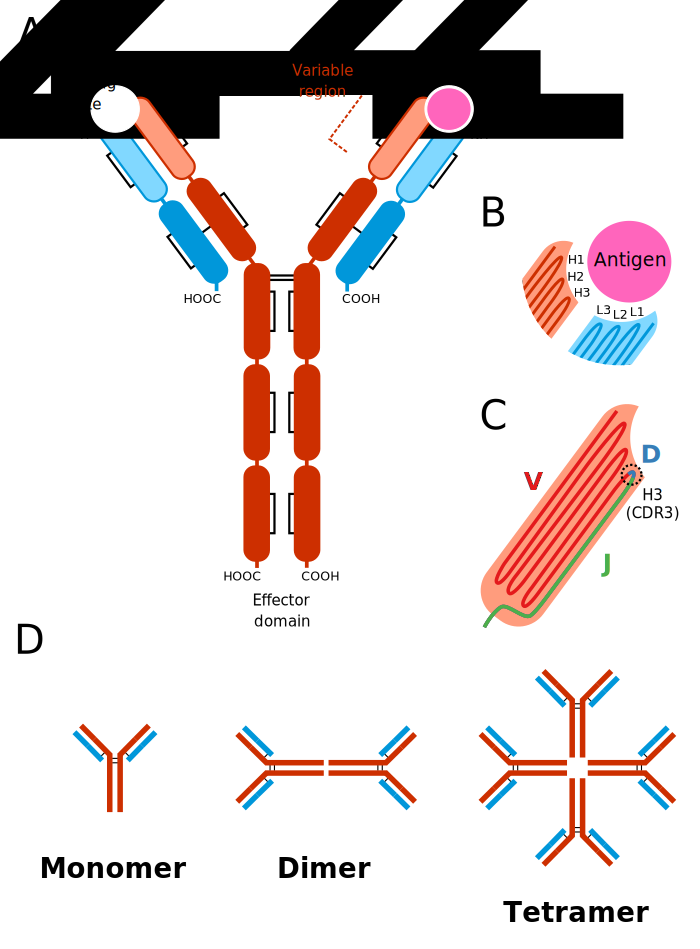
\includegraphics[width=0.9\textwidth]{output_files/figures/pdf/intro-antibody-structure}
\begin{subfigure}{0em}
\phantomsubcaption{}
\label{fig:intro-antibody-structure-schematic}
\end{subfigure}
\begin{subfigure}{0em}
\phantomsubcaption{}
\label{fig:intro-antibody-structure-loops}
\end{subfigure}
\begin{subfigure}{0em}
\phantomsubcaption{}
\label{fig:intro-antibody-structure-vdj}
\end{subfigure}
\begin{subfigure}{0em}
\phantomsubcaption{}
\label{fig:intro-antibody-structure-multimers}
\end{subfigure}
\Caption{Antibody structure and function}{(A) Schematic of a hingeless secreted antibody monomer, with heavy chains depicted in red, light chains in blue, and bound antigen in pink. Immunoglobulin fold domains are depicted as rounded rectangles, with variable-region domains shown with light shading and constant-region domains with dark. Black lines indicate disulfide bonds. (B) Schematic close-up of an immunoglobulin antigen-binding site, indicating the six loop regions (H1-3 and L1-3) making up the antigen-binding region. (C) Schematic close-up of the heavy-chain variable region, indicating the regions corresponding to the variable, diversity and joining gene segments from the unrecombined \igh{} locus. Note the chimeric nature of the third antigen-binding loop (H3, marked), which is formed by parts of all three gene segments. (D) In the context of antibodies, ``monomer'' refers to a single four-chain antibody protein, while ``dimer'', ``tetramer'' etc. refer to multiple four-chain monomers linked together through covalent or noncovalent interactions.}
\label{fig:intro-antibody-structure}
\end{figure}

\subsection{Antibody sequence diversification and primary repertoire diversity}
\label{sec:intro_immunity_primary}

The immune environment encountered by a vertebrate organism contains an enormous number of different potential pathogenic threats, each of which has its own antigenic signatures and many of which are capable of evolving much more rapidly than the vertebrate host \parencite{jack2015evolution}. In order for the adaptive immune system to cope with this huge diversity of different threats, it must be able to produce antibodies with a correspondingly large diversity of different antigen specificities. The greater the potential diversity of antibody sequences available to the adaptive immune system, the greater its capacity to respond effectively to novel immune threats. In fact, the mechanisms employed by the vertebrate adaptive immune system to diversify its antigen receptors enable an almost unlimited diversity of potential antibody sequences, with a correspondingly vast array of potential antigen specificities \parencite{mora2016diversity}.

The mechanisms by which the adaptive immune system produces this diversity are dramatic, and rely on a highly unusual underlying gene structure \parencite{jung2006vdjr} and a very high level of cellular wastage \parencite{kogut2012bcells}. In the humoral immune system, antibody diversification takes place during B-cell development in the primary lymphoid organs (bone marrow in mammals, anterior kidney in teleosts \parencite{sunyer2013fishing}). Prior to this process, the native antibody loci in B-progenitor cells (and other cell types) are highly fragmented \parencite{jung2006vdjr}, with numerous variable-region sequence segments present in series on the chromosome upstream of the constant-region exons. In the heavy chain locus, these variable-region gene segments can be divided into three categories:

\begin{itemize}
\item \textbf{Variable (\vh) segments} are the longest class of gene segment, at roughly \bp{300} in length \parencite{lefranc2003vnumbering}. Each \vh segment codes for the majority of the variable region of an antibody, including the entirety of the first three framework regions (FWR1-3) and the first two complementarity-determining regions (CDR1-2) as well as the 5' part of CDR3 \parencite{schroeder2010immunoglobulins,jung2006vdjr} (\Cref{fig:intro-antibody-structure-vdj}). They are therefore highly structured, and include several highly-conserved positions present in virtually all functional V-segments in nearly all species, including two conserved cysteine residues (which give rise to an intra-domain disulfide bond) and a conserved tryptophan residue following CDR1 \parencite{lefranc2003vnumbering}. Each V-segment is also associated with its own promoter sequence and 5'-UTR, as well as a 5'/C-terminal leader peptide between the translation start site and the start of the functional V-sequence.
\item \textbf{Diversity (\dh) segments} are the shortest class of segment, typically on the order of 10-\bp{20}, and are the least structured \parencite{ruiz1999humandj}. They form the middle part of CDR3 (\Cref{fig:intro-antibody-structure-vdj}) \parencite{schroeder2010immunoglobulins}.
\item \textbf{Joining (\jh) segments} are of intermediate length, typically 50-\bp{60} \parencite{ruiz1999humandj}. They form the 3'/C-terminal part of heavy chain CDR3 and the 5'/N-terminal part of FR4 (\Cref{fig:intro-antibody-structure-vdj}) \parencite{schroeder2010immunoglobulins}. Each J-segment is succeeded on the chromosome by a splice donor site \parencite{magadan2011medaka}, which is used to join the variable region of the antibody sequence to the constant region via RNA splicing following transcription of \igh{} mRNA (\Cref{fig:intro-vdjr-locus}iii). Like \vh segments, \jh segments can be identified from their conserved structure, particularly the conserved tryptophan residue marking the end of CDR3 \parencite{ruiz1999humandj}.
\end{itemize}

In the simplest ``translocon'' configuration of the \igh{} locus, blocks of repeated \vh, \dh and \jh segments are present in series on the chromosome in contiguous V-, D- and J-regions (\Cref{fig:intro-vdjr-locus}i) \parencite{schroeder2010immunoglobulins,jung2006vdjr}. During B-cell development, a single \vh, \dh and \jh segment are selected from these segment blocks, and the intervening genomic regions are permanently excised from the genome to produce a single, contiguous VDJ sequence coding for the complete variable region of an antibody (\Cref{fig:intro-vdjr-locus}ii). The mechanism by which this excision occurs is called VDJ recombination, and relies on a specialised recombinase complex containing lymphocyte-specific recombination-activating genes 1 and 2 (\gene{RAG1} and \gene{RAG2}) \parencite{jung2006vdjr,schatz2011vdjr}. This complex recognises specialised recombination signal sequences (RSSs) flanking each variable gene segment, composed of highly conserved heptamer and nonamer sequences separated by a spacer sequence of conserved length (either 12 or \bp{23}, corresponding respectively to one or two turns of the DNA helix) \parencite{hesse1989rss} (\Cref{fig:intro-vdjr-consensus}). Each functional \vh segment is succeeded by a \bp{23}-spacer RSS in 5'-3' orientation, while each \jh segment is preceded by a \bp{23}-spacer RSS in 3'-5' orientation; each \dh segment, meanwhile, is flanked by \bp{12}-spacer RSSs in 5'-3' and 3'-5' orientation, respectively (\Cref{fig:intro-vdjr-rss}) \parencite{schatz2011vdjr}. 

In VDJ recombination, recombinase complexes bind two of these RSSs and associate with each other to bring the two corresponding gene segments into close proximity (\Cref{fig:intro-vdjr-mechanism}i-iii). A single-strand DNA nick is introduced between each RSS and its gene segment, and the exposed 3'-hydroxyl group of the break attacks the 5'-phosphate on the other strand to produce an asymmetric double-strand break, with the coding sequence terminating in a hairpin loop and the cleaved RSS in a blunt end \parencite{schroeder2010immunoglobulins,schatz2011vdjr} (\Cref{fig:intro-vdjr-mechanism}iv-v). These breaks are then resolved by the ubiquitous non-homologous end-joining (NHEJ) machinery of the DNA damage response: the blunt ends of the cleaved RSSs can be directly ligated together, while for the coding sequences the hairpin loops must first be cleaved and the resulting 3'-overhangs resolved \parencite{schroeder2010immunoglobulins,schatz2011vdjr} (\Cref{fig:intro-vdjr-mechanism}vi-vii). The net result of this process is a contiguous V/D or D/J join in the coding sequence and a ligated DNA circle containing the excised RSSs and intervening sequence, which is subsequently degraded. Via unknown mechanisms \parencite{schatz2011vdjr}, the recombination machinery exhibits a strong preference for RSS sequences of different lengths (the so-called ``12/23 rule''), encouraging  D-J and V-D joins while largely preventing V-J joins. 

The simple joining of gene segments during VDJ recombination provides a basic combinatorial sequence diversity, with a number of possible sequences in the simplest case equal to the product of the numbers of \vh, \dh and \jh segments in the \igh{} gene locus. The number of potential \igh{} variable-region sequences in most species, however, is vastly higher than this: in humans, for example, there are roughly 8000 possible functional VDJ combinations \parencite{lefranc2001humanheavy}, but the number of different possible nucleotide sequences exceeds $10^{21}$ \parencite{elhanati2015model}. This huge difference arises from the inexactness with which the coding ends produced by the recombinase complex are joined following RSS excision (\Cref{fig:intro-vdjr-junctions}). Before the two gene segments brought together in VDJ recombination can be joined by NHEJ, the hairpin loops formed by the recombinase complex must be resolved by re-nicking the DNA \parencite{schroeder2010immunoglobulins,schatz2011vdjr}. This re-nicking process is not exact, and often occurs within the coding sequence, resulting in a palindromic 3'-overhang that can be filled in (resulting in palindromic \textit{P-insertions}) or trimmed (resulting in \textit{deletions}). The resulting blunt ends then serve as substrates for the lymphocyte-specific terminal dideoxy transferase enzyme (TdT), which adds a variable number of untemplated nucleotides (nonpalindromic \textit{N-insertions}) prior to sequence ligation \parencite{schroeder2010immunoglobulins,schatz2011vdjr}. As a result, the final recombined sequence is frequently not a clean ligation of the two original gene segments, but an inexact join involving multiple missing terminal positions and/or \textit{de novo} inserted nucleotides, a phenomenon collectively known as \textit{junctional diversity} \parencite{flaherty2012chapter}.

The three processes contributing to junctional diversity (P-insertion, N-insertion, and deletion) together vastly increase the potential antibody sequence diversity available to a developing B-cell at the heavy-chain CDR3 region, which as a consequence is by far the most important single region on either antibody chain in determining antigen specificity \parencite{shirai1999h3}. This junctional diversity, however, comes at a substantial cost. The indel mutations introduced by VDJ recombination are not constrained to occur in multiples of three over both junctions, resulting in a high rate of recombinations in which the \vh and \jh segments are out of frame with each other; still more loci are rendered nonfunctional through the introduction of \textit{de novo} stop codons. As the sequence changes introduced by VDJ recombination are irreversible, many developing B-cells are left with permanently disrupted \igh{} loci on both chromosomes, and are left with no recourse but programmed cell death. In addition, the huge and untemplated sequence diversity introduced in this way means that many B-cells whose \igh{} loci do successfully undergo VDJ recombination are left with BCRs that either cannot effectively bind any antigen or strongly bind self-antigen, resulting in useless antibodies in the first case and a dangerous risk of autoimmunity in the second; these B-cells are eliminated through a process of antigenic selection before \naive B-cells are permitted to exit the primary lymphoid organs, resulting in still more wastage as cells with nonfunctional or self-binding antigens undergo programmed cell death. Overall, as many as 90\,\% of developing B-cells may be eliminated by one or other of these processes before successfully exiting to the periphery \parencite{kogut2012bcells}.  

Taken together, the processes of VDJ recombination, junctional diversity and primary selection will produce a population of \naive B-cells with an extremely high diversity of heavy-chain ideotypes, with virtually every \naive B-cell expressing a unique variable-region sequence. Taken together, the resulting population of sequences represents the \textit{primary antibody heavy-chain repertoire} of the organism, and determines the range of different antigen sequences the humoral immune system of that organism can potentially respond to. The diversity of this primary repertoire depends on the native structure of the \igh{} locus in that species (which determines the number of segment choices available to the VDJ-recombination process), the distribution of possible numbers of insertions or deletions contributing to junctional diversity, and the stringency of the primary-selection process.

\begin{figure}
\centering
\includegraphics[width=0.95\textwidth]{output_files/figures/pdf/intro-primary-diversity}
\begin{subfigure}{0em}
\phantomsubcaption{}
\label{fig:intro-vdjr-locus}
\end{subfigure}
\begin{subfigure}{0em}
\phantomsubcaption{}
\label{fig:intro-vdjr-consensus}
\end{subfigure}
\begin{subfigure}{0em}
\phantomsubcaption{}
\label{fig:intro-vdjr-rss}
\end{subfigure}
\begin{subfigure}{0em}
\phantomsubcaption{}
\label{fig:intro-vdjr-mechanism}
\end{subfigure}
\begin{subfigure}{0em}
\phantomsubcaption{}
\label{fig:intro-vdjr-junctions}
\end{subfigure}
\Caption{Primary sequence diversification in the immunoglobulin heavy chain}{(A) Schematic of antibody sequence formation at the locus level. Black asterisks indicate the segments to be recombined. (B) Consensus sequence of short (above) and long (below) RSSs in jawed vertebrates. Nucleotides marked in red are the most strongly conserved and most required for efficient recombination \parencite{hesse1989rss}. (C) Schematic of position and orientation of long (yellow) and short (purple) RSSs relative to variable-region gene segments. (D) Schematic of recombination mechanism for a D/J segment pair, illustrating hairpin formation and imprecise end-joining of coding sequences; adapted from \parencite{schatz2011vdjr}, Figure 2. (E) Example of the inexact hairpin resolution mechanisms leading to junctional diversity in (D-vi); adapted from \parencite{flaherty2012chapter}, Figure 10-5.}
\label{fig:intro-vdjr}
\end{figure}

\subsection{\igh{} locus structure in teleost fishes}
\label{sec:intro_teleost_loci}

\Cref{sec:intro_immunity_primary} describes the process of \igh{} locus maturation in terms of an idealised translocon locus with a simple V-D-J-C structure (\Cref{fig:intro-vdjr-locus}). In some species, including humans and mice, \igh{} loci roughly correspond to this layout \parencite{jung2006vdjr}; however, in many species, including all teleosts, this idealised structure is a significant oversimplification of the actual layout of their \igh{} loci \parencite{fillatreau2013astonishing}. Due to their size, repetitiveness and complexity, comprehensive assembly of \igh{} loci is often difficult, and full elucidation of their structure often requires a focused characterisation effort. Nevertheless, a number of teleost loci have been characterised to date, primarily from species used widely in research (e.g. zebrafish, medaka, stickleback), agriculture (e.g. salmon, grass carp, channel catfish) or both (e.g. rainbow trout) \parencite{fillatreau2013astonishing,bengten2015fishantibodies}.

Among teleost fishes, the simplest \igh{} locus structures known to date are exhibited by species such as zebrafish, grasscarp, and fugu (\Cref{fig:intro-teleost-loci-simple}) \parencite{fillatreau2013astonishing}. In these species, the \igh{} locus adopts a V-D-J-\cz{}-D-J-\cm{}-\cd{} structure, with a single shared V-region followed by D- and J-regions specific to the \igh{Z} and \igh{M/D} constant regions, respectively. The rainbow trout locus has a similar organisation, but with two additional \vh segments following the \igh{Z} region \parencite{hansen2005trout}. During VDJ recombination in these loci, the choice of variable gene segments also determines the choice of constant region: if a pair of \dh and \jh segments upstream of the \igh{Z} constant region is selected, the cell will express \igh{Z}, while if the segments chosen are downstream of \igh{Z}, that constant region will be excised during VDJ recombination and \igh{M} and/or \igh{D} will be used instead. As a result, VDJ recombination in these species determines both the ideotype of a developing B-cell and its isotype \parencite{fillatreau2013astonishing}.

While some teleost species possess such relatively simple \igh{} loci, many species exhibit much more complicated, and often much larger, locus structures. In many species, multiple distinct subloci (comprising V-, D- and J-regions and least one constant region) are present in tandem on the chromosome, often with distinct combinations of variable gene segments and constant regions (\Cref{fig:intro-teleost-loci-complex}); in a few cases, such as medaka and Atlantic salmon, one or more of these subloci is in inverted orientation relative to the rest of the locus. In some species, such as Atlantic salmon, whole-genome duplication has led to the existence of multiple distinct \igh{} loci on different chromosomes, each of which has its own complement of subloci, gene segments, and constant regions \parencite{yasuike2010salmon}. In this milieu, pseudogenisation of gene segments or constant-region exons is common, resulting in loci with large numbers of pseudogenised V-segments and constant regions.

The diversity in locus size and organisation among teleost fishes is likely to have important consequences for humoral adaptive immunity in these species. The native locus constitutes the raw substrate for the VDJ recombination process, and the number of different \vh, \dh and \jh gene segments available for recombination defines the baseline sequence diversity of antibodies in that species. It is not clear to what extent VDJ recombination can take place across different subloci in the large tandem loci described in \Cref{fig:intro-teleost-loci-complex}; if recombination between subloci is restricted, this will also have important effects on the kinetics of VDJ recombination in a species. The division of an \igh{} locus into tandem subloci may also have effects on the statistics of B-cell maturation, with more subloci conceivably presenting the opportunity for a greater number of recombination attempts before the \igh{} loci of a developing B-cell are exhausted and so reducing the rate at which cells fail to mature successfully; however, to my knowledge little or nothing is known about the effects of locus structure on B-cell developmental processes at present. Finally, variations in the constant regions present in different species are likely to have very important effects on humoral immunity; most fundamentally, whereas \igh{Z/T} appears to be specialised for mucosal adaptive immunity in those teleost species that possess it \parencite{zhang2010igtgut,fillatreau2013astonishing,xu2013igtskin}, it is not known how mucosal immune responses manifest in teleost species lacking this isotype. Given all these important (and potentially-important) effects of \igh{} locus structure on humoral adaptive immunity, characterising the sequence and organisation of this locus is an essential step in understanding the adaptive immune system of any given vertebrate species.

\begin{figure}
\centering
\includegraphics[width=0.85\textwidth]{output_files/figures/pdf/intro-teleost-loci}
\begin{subfigure}{0em}
\phantomsubcaption{}
\label{fig:intro-teleost-loci-simple}
\end{subfigure}
\begin{subfigure}{0em}
\phantomsubcaption{}
\label{fig:intro-teleost-loci-complex}
\end{subfigure}
\Caption{\igh{} locus structure in teleost fishes}{Simplified schematics of \igh{} loci from nine teleost species. (A) In the simplest teleost \igh{} loci, single \igh{Z} and \igh{M/D} constant regions share a common V-region, but are preceded by separate D/J regions. In rainbow trout, a small number of V-segments also separate \igh{Z} from the pre-\igh{M} D-region. (B) In many teleosts, the \igh{} loci are much larger and more complex, with repeated tandem subloci (labelled regions), pseudogenised constant regions (grey, $\psi$), inverted segments (leftward arrows), and other deviations from the classic locus organisation. Loci are not to scale; blocks of more than five segments are condensed and labelled with their segment number, as are some smaller segment blocks for clarity. Adapted from \parencite{fillatreau2013astonishing}, Figure 2 and \parencite{bengten2015fishantibodies}, Figure 4, with additional information from \parencite{magadan2011medaka,bao2010stickleback,gambondeza2011stickleback,yasuike2010salmon,xiao2010grasscarp}.
The number of D-regions in the medaka locus is not provided in the sources.}
\label{fig:intro-teleost-loci}
\end{figure}

\subsection{Affinity maturation and secondary repertoire diversity}
\label{sec:intro_affinity_maturation}

Following VDJ recombination and primary selection, developed \naive B-cells emerge from the primary lymphoid organs and circulate in the periphery. At some point, a subset of these \naive cells will make contact with their cognate antigen. If this contact occurs in the correct signalling context (e.g. in the presence of T-cell help for T-dependent responses \parencite{sompayrac2019immune}), the B-cell becomes activated and begins to proliferate \parencite{dunnwalters2010bcellageing}. During this clonal expansion process, the B-cell's antibody genes undergo a very high rate of somatic mutation (known as \textit{somatic hypermutation} or SHM), with mutations focused in the complementarity-determining regions coding for the antigen-binding loops of the variable region; in mammals, the rate can be as high as $10^{-3}$ per nucleotide per cell division \parencite{noia2007shm}. This SHM process is orchestrated by the activation-induced cytidine deaminase enzyme (AID), which preferentially targets particular hotspot motifs and deaminates cytidine residues to uracil, which can either be corrected to thymine on DNA replication (resulting in a C-to-T transition mutation) or removed via base-excision repair (resulting in a variety of other mutations) \parencite{magor2015affinity}. As a result, the original antibody sequence of the ancestral \naive cell is diversified into a cluster of related sequences, with widely varying affinity for the cognate antigen.

In order for the combination of clonal expansion and somatic hypermutation to improve the adaptive immune system's ability to respond to the stimulating antigen, the resulting clone needs to undergo a selection process, to identify and favour cells expressing antibodies with improved antigen affinity. This selection is effected through a competitive process in which clonally-expanded B-cells attempt to bind cognate antigen trapped on the surface of helper cells: those cells which successfully bind antigen receive growth and differentiation signals, while those which do not undergo programmed cell death. In mammals, this process takes place primarily in histologically-distinct germinal centres within specialised secondary lymphoid organs such as the spleen \parencite{victora2012gc}, in which B-cells that have encountered antigen first undergo clonal expansion and SHM, then compete for antigen on the surface of follicular dendritic cells (FDCs) \parencite{howard2006quality,victora2012gc}. In teleosts, which lack specialised, histologically-differentiated germinal centres, B-cell proliferation takes place near clusters of melanomacrophages surrounded by reticular cells, both of which have been attributed an antigen-trapping and -presentation role analogous to that performed by FDCs in mammals \parencite{magor2015affinity}.

While clonal expansion, somatic hypermutation and clonal selection, collectively known as \textit{affinity maturation}, are present in both mammals and teleosts, the increase in antibody affinity resulting from this process in teleosts is much weaker than in mammals (e.g. 3-to-10-fold in rainbow trout, compared to as much as 1000-fold in mammals \parencite{magor2015affinity}). Since SHM appears to be fully functional in those fish so far investigated \parencite{magor2015affinity}, this difference seems likely to arise from differences in clonal-selection dynamics between teleosts and mammals. The reasons for such a difference are still not entirely clear, but may involve histological differences in where and how affinity maturation takes place in these taxa. In mammalian germinal centres, the ratio between expanded B-cells and FDCs is such that the amount of presenting antigen is limiting, forcing competition for antigen among B-cells and favouring those cells which can bind antigen most strongly \parencite{magor2015affinity}. In teleosts, conversely, proliferating B-cells are far outnumbered by antigen-trapping melanomacrophages and reticular cells, resulting in an oversupply of antigen relative to B-cell demand; this antigen surplus may result in faster overall proliferation, but at the cost of much weaker selection for high-affinity antibodies \parencite{magor2015affinity}.

Following affinity maturation, activated B-cells undergo differentiation into memory cells (which persist in the bloodstream for long periods and provide secondary immune memory) \parencite{victora2012gc,mayer2018memory} and plasmablasts/plasma cells (which secrete large amounts of antigen to mount a powerful immune response) \parencite{howard2006quality,dunnwalters2010bcellageing,victora2012gc}. Affinity-matured cells can also re-enter germinal centres (or their less-developed teleost equivalents) to undergo additional rounds of proliferation, hypermutation and selection \parencite{howard2006quality,victora2012gc}; memory cells can also undergo further rounds of affinity maturation, resulting in even larger and more diverse clones and still-higher levels of antigenic affinity. In tetrapods, class switching between different constant-region isotypes also occurs as part of affinity maturation, and is also orchestrated by AID; however, this process appears to be absent in teleosts \parencite{magor2015affinity}.

The combination of the primary (\naive) repertoire described in \Cref{sec:intro_immunity_primary} with the clonal expansions and additional sequence diversity arising from affinity maturation constitutes the \textit{secondary heavy-chain antibody repertoire} of the organism (\Cref{fig:intro-bcell-repertoires}). This is the repertoire actually encountered by incoming pathogens and available to relatively direct experimental interrogation. The structure and diversity of this secondary repertoire depends on the makeup of the primary repertoire, the degree of clonal expansion and hypermutation during affinity maturation, the strength of clonal selection, and the relative abundance of different B-cell subtypes. Inferring the composition of the primary repertoire from that of the secondary is therefore non-trivial, and requires an attempt to distinguish sequences arising from \naive vs activated B-cells or infer the former from the latter; once obtained, the \naive sequences can be used to infer the parameters of the generative process \parencite{elhanati2015model,marcou2018igor}.

\begin{figure}
\centering
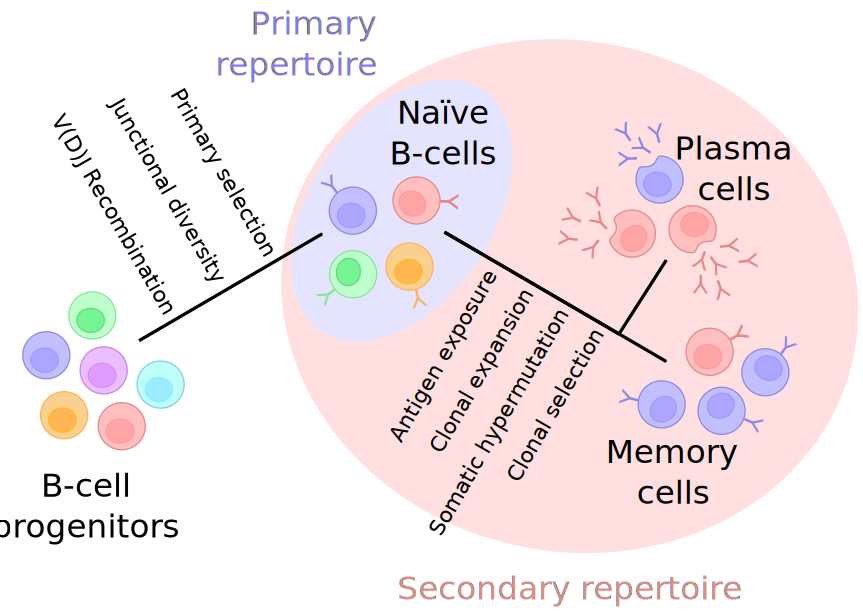
\includegraphics[width=0.9\textwidth]{output_files/figures/pdf/intro-bcell-repertoire-primary-secondary}
\Caption{Primary and secondary antibody repertoires}{Schematic of processes giving rise to the primary (\naive) and secondary (total) B-cell repertoires in the vertebrate immune system. Cell colours indicate clonal membership, with a loss of clonal diversity during primary development (left) and affinity maturation (right). Primary B-cell development (left) takes place in primary lymphoid organs (bone marrow in mammals, anterior kidney in teleosts \parencite{sunyer2013fishing}), while affinity maturation (right) takes place in germinal centres (in mammals) or proto-germinal clusters (in teleosts) in secondary lymphoid organs such as the gut-associated lymphoid tissue (GALT) or spleen \parencite{victora2012gc,magor2015affinity}.}
\label{fig:intro-bcell-repertoires}
\end{figure}

\section{Humoral adaptive immunosenescence in jawed vertebrates}
\label{sec:intro_immunosenescence}

The immune system of aged vertebrates has long been known to undergo a severe and systemic decline in functionality with age \parencite{segre1977immunosenescence}. As a result of this decline, older individuals exhibit increased susceptibility to a wide range of bacterial, viral, and fungal infectious diseases, as well as higher rates of complications and mortality from those infections when they occur \parencite{sambhara2009vaccination}. In addition, the effectiveness of vaccination against these infections often declines dramatically with age, with older individuals often receiving half or less of the immune protection from vaccination exhibited by younger recipients \parencite{sambhara2009vaccination}. Similar declines in immune functionality with age are also observed in other model organisms, and have been especially well-studied in mice, which share many details of their immune system with humans while being substantially easier to study in depth. While many different parts of the immune system are implicated in this immunosenescent phenotype \parencite{kogut2012bcells}, the decline in the humoral adaptive immune system has emerged as one particularly important contributor \parencite{ademokun2010ageing}.

The changes in the humoral immune system underlying its impaired functionality in old age begin at the level of B-cell development. In mice, the population of haematopoietic stem cells (HSCs) resident in the bone marrow increases in number but exhibits a decreased propensity to regenerate the pool of developing B-cells \parencite{ademokun2010ageing,kogut2012bcells}; factors contributing to this change include a deteriorating bone marrow niche, changes in blood-borne factors affecting HSC differentiation, and the well-known bias of older mammalian HSCs towards myeloid (rather than lymphoid) cell lineages \parencite{kogut2012bcells,dunnwalters2010bcellageing}. As a result of this change in HSC behaviour, the number of new B-cell progenitor and precursor cells in the bone marrow declines with age in mice; furthermore, these precursors exhibit decreased proliferation capacity, reduced rates of VDJ recombination and an increased rate of apoptosis \parencite{montecino2013immunosenescence,kogut2012bcells,labrie2004bone}. The rate of B-cell output from the bone marrow therefore declines significantly in aged mice, falling as low as 10\,\% of its level in young adults \parencite{kogut2012bcells}. As these \naive cells also have a shorter lifespan than antigen-experienced memory- and long-lived-plasma-cell populations, the net result of this decline in output from the bone marrow is a decrease in the number of \naive cells in the periphery and a progressive increase in the relative prevalence of antigen-experienced memory and plasma cells \parencite{mehr2011reversing,kogut2012bcells}; the pool of circulating immunoglobulins, meanwhile, becomes progressively dominated by hypermutated antibodies specific to previously-encountered antigens \parencite{kogut2012bcells}. As the \naive{}-cell pool is essential for responding to pathogenic threats not previously encountered by the immune system, this change is thought to lead to a progressive reduction in the capacity of the humoral immune system to respond effectively to these novel threats \parencite{kogut2012bcells}.

Despite the decline in new \naive B-cells produced by the bone marrow, the total number of B-cells in aged mice does not appear to change significantly, reflecting an increase in the absolute number, as well as the relative prevalence, of antigen-experienced B-cell subpopulations \parencite{ademokun2010ageing}. In humans, conversely, the absolute number of total B-cells appears to decline with age \parencite{ademokun2010ageing,montecino2013immunosenescence,aberle2013mechanistic}, with most B-cell subsets showing a significant decline in absolute abundance \parencite{frasca2011age}. Sources differ as to the age-related changes in relative abundance of different B-cell subtypes in humans, with some reporting an increase in the relative prevalence of \naive cells and decrease in that of memory cells \parencite{frasca2011age,blomberg2013age} and others reporting a more mouse-like shift in favour of the memory compartment \parencite{ademokun2010ageing}. These differences may arise from differences in the methods and cell markers used to quantify abundance of different B-cell populations \parencite{ademokun2010ageing}, genuine differences between populations, or the limitations of peripheral blood as a method of sampling the whole-body B-cell population of an individual \parencite{siegrist2009extremes,tabibiankeissar2016ageing}.

Whatever changes in cellular composition occur in ageing humans, it is clear that both humans and mice undergo a severe age-related decline in B-cell functionality. In humans, the best-understood aspect of this decline is a deterioration in the responsiveness of older patients to vaccination. Older humans frequently exhibit a substantially smaller \parencite{sambhara2009vaccination} and slower \parencite{kogut2012bcells} increase in the titre of antigen-specific serum antibodies in response to vaccination \parencite{sasaki2011limited,aberle2013mechanistic,ademokun2010ageing}, with defects in humoral response observed to vaccines for diseases as diverse as influenza, hepititis A and B, tetanus, diphtheria, pneumococcus and tick-borne encephalitis \parencite{dunnwalters2010bcellageing}. At least in the case of influenza, the observed decline in specific antibody production is primarily due to a decrease in the number of plasmablasts activated in response to vaccination \parencite{montecino2013immunosenescence,aberle2013mechanistic,sasaki2011limited}.

In addition to being less abundant, the antibodies produced by elderly humans in response to vaccination also appear to be of lower quality: anti-influenza antibodies produced by older human individuals demonstrate reduced ability to effectively neutralise viral haemagglutinin \parencite{kogut2012bcells,sasaki2011limited}, while \igh{M} antibodies produced by elderly subjects in response to pneumococcal polysaccharide vaccine demonstrate reduced opsonisation ability \parencite{kogut2012bcells}. While basal serum antibody titres actually increase with age in humans and mice \parencite{frasca2009ageing}, suggesting that antibody production \textit{per se} is not impaired, these antibodies also decline in quality \parencite{montecino2013immunosenescence}, with measurable increases in the rate of polyspecific and self-reactive antibodies produced in older individuals \parencite{kogut2012bcells}. This decline in baseline antibody quality in older individuals suggests a breakdown in primary B-cell selection in the bone marrow, enabling a greater number B-cells with low-specificity or self-reactive antibody sequences to emerge into the periphery \parencite{ademokun2010ageing}.

Various aspects of affinity maturation are also impaired in aged mammals. While memory-cell clones established early in life often persist into old age, \naive B-cells in aged humans demonstrate a severely reduced ability to give rise to new antigen-specific memory B-cells following antigenic stimulation, impairing the establishment of functional immune memory for novel threats \parencite{aberle2013mechanistic}. B-cells from older humans and mice also exhibit impaired class-switch recombination capacity, possibly as a result of decreased AID expression \parencite{montecino2013immunosenescence,blomberg2013age,frasca2011age}, impairing the generation of antibodies with the same specificity but different effector functions. The decreased ability of older individuals to produce high-affinity antigen-specific antibodies \parencite{frasca2011age} also suggests a defect in affinity maturation, though this could also be attributable to the known ageing-related defects in the T-helper and follicular dendritic cells involved in secondary B-cell selection \parencite{montecino2013immunosenescence,aberle2013mechanistic,ademokun2010ageing} rather than changes in the B-cells themselves. Conversely, the effect of ageing on the somatic hypermutation process remains controversial \parencite{henry2019influenza,howard2006quality,ademokun2010ageing,frasca2009ageing}, with different groups reporting an increase, a decrease, or no change in the rate and level of SHM accumulation of different B-cell subtypes with age. 

The various cellular and population-level changes that occur in the humoral immune system with age naturally have important effects on the antibody repertoires of ageing individuals. Aged humans \parencite{siegrist2009extremes} and mice \parencite{dunnwalters2010bcellageing} exhibit increased rates of non-malignant clonal expansions in the memory-cell compartment, which when combined with the apparent maintenance or decline in total B-cell number would lead to a reduction in overall diversity \parencite{dunnwalters2010bcellageing}. Similarly, early techniques that investigated the repertoire by investigating the distribution of CDR3 lengths (CDR3 spetratyping) indicated that older humans frequently exhibit more distorted distributions dominated by CDR3 regions of a particular length, indicative of clonal expansion, and found that older individuals with more distorted spectratypes exhibited greater frailty and worse health and lifespan outcomes than those with more young-like spectratypes \parencite{gibson2009spectratyping}. On the basis of these and similar findings, the antibody repertoire has long been thought to decline in diversity in older individuals, impairing the adaptability of the ageing adaptive immune system.

More recently, the development of specialised high-throughput-sequencing-based techniques for interrogating antibody repertoires (\Igseq, or \igseq \parencite{weinstein2009igseq,georgiou2014promise}) has enabled a few studies to investigate the ageing of these repertoires in greater detail. These studies, primarily on human peripheral blood, have confirmed many observations made using older lower-throughput methods: a reduced number of clonal lineages in older repertoires supports a decrease in \naive-cell output from the bone marrow \parencite{jiang2013vaccine}, while an increase in mean CDR3 length \parencite{wang2014ageing} and the rate of premature stop codons \parencite{debourcy2017ageing} support the finding that primary and clonal selection are impaired with age. An increase in clonal expansion with age is also observed in sequencing data: an oligoclonal phenotype, in which one or a few large clones dominate the repertoire, is often seen in peripheral blood from elderly humans but very rarely in the young \parencite{wang2014ageing,debourcy2017ageing}. These expanded clones are persistent before and after vaccination \parencite{debourcy2017ageing} and even across multiple years \parencite{wang2014ageing}; in contrast, large clones observed in young human blood repertoires are typically transient responses to recent antigen challenge \parencite{wang2014ageing}.

The reduction in clonal richness and increase in clonal expansions seen in older individuals contribute to an overall reduction in the estimated number of unique sequences present in the peripheral repertoire \parencite{debourcy2017ageing}, a change observed for both \naive and mutated sequences. The same study also found a drop in the percentage of unique sequences identified as coming from \naive B-cells, suggesting a mouse-like shift in repertoire prevalence towards antigen-experienced cell types \parencite{debourcy2017ageing}. However, while the alpha (within-individual) sequence diversity of the human peripheral repertoire appears to decline with age, the beta (between-individual) diversity of the repertoire actually increases, with repertoires from older individuals differing more from one another than those from young individuals do \parencite{debourcy2017ageing}. Elderly repertoires also showed decreased flexibility in response to immune challenge, with repertoires taken from the same individual pre- and post-vaccination being significantly more similar in elderly than in young samples \parencite{debourcy2017ageing}. Taken together, these findings suggest a pattern in which human peripheral antibody repertoires progressively lose diversity and flexibility over the course of the human lifespan, while also becoming increasingly individualised and distinct.

In conclusion, there is strong evidence for a variety of cellular and physiological changes in the B-cell immune system with age in both mice and humans, giving rise to a severe decline in functional performance and immune protection. Many of these changes affect the composition of the antibody repertoire, with a reduction in clonal and sequence diversity and an increase in between-individual variability with age in human blood. However, despite this abundance of data, there remain some serious limitations in our knowledge of the ageing antibody repertoire.  From an evolutionary and comparative perspective, almost nothing is known about adaptive immunosenescence in species other than humans and mice; while several \igseq studies have been performed on teleost fish \parencite{weinstein2009igseq,jiang2011determinism,krasnov2017igseq,lund2019salmon,fu2018fugu}, for example, none to my knowledge have investigated B-cell immunosenescence in this taxon. Many of the findings reported above are specific to \igh{G} or \igh{A} antibodies in mice and humans \parencite{kogut2012bcells}, and may not generalise to species lacking these isotypes. Even in humans, the majority of immunosenescence studies, including virtually all repertoire studies, are limited to peripheral blood, and therefore primarily sample the minority of B-cells in transition between tissues; the majority of B-cells, which are resident in some immune organ or tissue, are systematically underrepresented in these samples \parencite{siegrist2009extremes,tabibiankeissar2016ageing}. Relatively little is therefore known about how the ageing of the B-cell repertoire differs between organs; the only paper I know of which investigated changes in antibody-repertoire diversity with age in biopsies from multiple human tissues failed to find any significant changes in alpha diversity, except for a significant \textit{increase} in repertoire sequence entropy in old spleen \parencite{tabibiankeissar2016ageing}. To my knowledge, no publication has yet investigated the ageing of the antibody repertoire at mucosal surfaces, where secreted antibodies play a particularly important role in regulating microbiotal communities and defending the body from pathogenic invasion \parencite{belkaid2014microbiota}.

In addition to this lack of spatial resolution in our knowledge of antibody repertoire ageing, there is a serious lack of temporal resolution; most studies of antibody repertoire ageing simply compare a ``young'' group (say 20-30 years of age) with one or two ``old'' groups (say $\geq70$ years of age), with little or no information about the intervening progression of any observed phenotypes \parencite{debourcy2017ageing,tabibiankeissar2016ageing}. The effect of known lifespan-increasing interventions on immune-repertoire ageing also remains largely unstudied. Due to their very long lifespans and restrictions on experimental manipulation, humans are unsuitable subjects for these sorts of experiments, as are long-lived vertebrate model organisms such as zebrafish (median lifespan c. 3.5 years \parencite{gerhard2002zebrafish}) and \textit{Xenopus} (median lifespan c. 9 years \parencite{bowler1977longevity}). Even mice, though widely used in biogerontology, are inconveniently long-lived for many ageing experiments (median lifespan c. 2 to 2.5 years for the most common laboratory strains \parencite{yuan2009aging}). Conversely, many major model organisms in ageing research (such as fruit flies and nematode worms) are invertebrates, and so lack a mammal-like adaptive immune system. The development of a short-lived vertebrate species as a model organism for antibody-repertoire experiments would therefore be highly valuable for research into adaptive immunosenescence.

\section{The African turquoise killifish as a model for vertebrate ageing}
\label{sec:intro_killifish}

The genus \textit{Nothobranchius} comprises a broad group of annual freshwater fishes distributed across equatorial and subequatorial Africa \parencite{valdesalici2003lifespan}, with species diversity concentrated in the south-east of the continent \parencite{genade2005annual}. Members of this genus share a suite of adaptations to life in ephemeral pools and rivers, most notably the production of desiccation-resistant embryos capable of surviving through the dry season in a diapause state \parencite{genade2005annual} (\Cref{fig:intro-killifish-life-cycle}). Fish from this genus have been known for several decades to  exhibit very rapid growth and short lifespans, consistent with their evolving under conditions of very high extrinsic mortality \parencite{valdesalici2003lifespan}, with many species exhibiting a median lifespan of less than one year. Nevertheless, there is wide variation within the genus in body size, growth rate and lifespan, with species from less arid regions tending to show slower growth and longer median lifespans \parencite{genade2005annual}.

Like other \textit{Nothobranchius} species, the turquoise killifish (\nfu, \Cref{fig:intro-killifish-photos}) is a medium-sized annual fish first isolated from ephemeral freshwater pools -- in this case, from a relatively arid region of southeastern Zimbabwe and Mozambique \parencite{genade2005annual,jubb1971new}. Even by the standards of the \textit{Nothobranchius} genus, \Nfu exhibits extremely rapid growth, maturation, and ageing, with the most widely-used laboratory strain (GRZ) exhibiting a median lifespan of just 9-16 weeks \parencite{valdesalici2003lifespan,genade2005annual,terzibasi2008strains,kirschner2012map,valenzano2015genome,smith2017microbiota} (\Cref{fig:intro-killifish-lifespan}) -- the shortest lifespan of any captive-bred vertebrate, and a dramatic outlier on the distribution of vertebrate lifespans (\Cref{fig:intro-killifish-comparison}). Combined with their possession of several important vertebrate-specific adaptations -- including an adaptive immune system -- this extremely short lifespan makes the turquoise killifish a highly promising model organism for ageing research \parencite{harel2016crispr}.

Despite its very short lifespan, \textit{N. furzeri} has been found to show a wide range of senescent phenotypes in even the shortest-lived strains, including lipofuscin deposition \parencite{genade2005annual};  accumulation of senescence markers \parencite{genade2005annual};  increased neurodegeneration \parencite{valenzano2006resveratrol1,valenzano2006resveratrol2}; impaired learning and behavioural phenotypes  \parencite{genade2005annual,valenzano2006resveratrol1}; and a high incidence of degenerative and neoplastic lesions \parencite{dicicco2011histopathology}. These diverse phenotypes indicate that the short lifespan of the turquoise killifish is the result of an accelerated general ageing process, rather than the specific failure of a particular organ or system. Moreover, established anti-ageing interventions such as resveratrol treatment \parencite{valenzano2006resveratrol1}, reduction in ambient temperature \parencite{valenzano2006temperature} and dietary restriction \parencite{terzibasi2009dr} also extend lifespan in the turquoise killifish, indicating a strong analogy with the ageing phenotypes observed in canonical model systems.

Due primarily to its potential as a model organism for ageing research, the turquoise killifish has also seen rapid development as a genetic model. The short-lived GRZ strain has been bred in captivity for fifty years and at least a hundred generations \parencite{terzibasi2007review} and exibits a very high degree of homozygosity \parencite{kirschner2012map,reichwald2009genome,valenzano2009map}, providing a uniform genetic background for experimental interventions. A number of important genetic resources are now available, including several assemblies of the nuclear genome \parencite{reichwald2015genome,valenzano2015genome,willemsen2019popgen}, the most recent of which \parencite{willemsen2019popgen} is of very high quality. These assemblies have yielded a genome with an estimated size of roughly 1.5 gigabases \parencite{willemsen2019popgen};
karyotyping \parencite{reichwald2009genome} and sequencing analysis \parencite{reichwald2015genome} both indicate a chromosome number of $2n = 38$, corresponding to 19 distinct linkage groups in the haploid genome.

Prior to the work contained in this thesis, almost nothing was known about the adaptive immune system of the turquoise killifish. However, as a teleost, and therefore as a jawed vertebrate, it could be strongly expected to have a roughly mammal-like adaptive immune system, and a number of genes related to B-cell adaptive immunity (including \gene{RAG1}, various B-cell developmental markers, and fragments of antibody genes) were identified in one or more genome annotations. Phylogenetically, the genus \textit{Nothobranchius} falls within the Cyprinodontiformes, and the turquoise killifish is therefore relatively closely related to several species with previously-characterised \igh{} loci, including fugu, stickleback and medaka \parencite{terzibasi2007review,hughes2018teleostphylo}. Despite the relatively unknown state of adaptive immunity in the turquoise killifish, therefore, there was good reason to believe it possessed a functional B-cell immune system similar to those of other teleosts, and therefore comparable in many respects with those of mammalian species, including humans. When combined with its short lifespan and rapid ageing phenotype, this made the turquoise killifish a potentially highly-valuable model for studying the forms and mechanisms of humoral adaptive immunosenescence in jawed vertebrates. % TODO: Break paragraph here? (If relating findings)

In this thesis, therefore, I characterised the \igh{} locus of the turquoise killifish (\Cref{chap:locus}), established a working \Igseq protocol for killifish samples, and performed the first experiments investigating adaptive immunosenescence in this species (\Cref{chap:igseq}). The results demonstrated that turquoise killifish possess a complex and sophisticated adaptive immune system with diverse and individualised antibody repertoires, which nevertheless undergoes a rapid loss of within-individual diversity with age. This loss of diversity was especially pronounced in isolated gut samples, possibly due to the intense antigenic exposure experienced at mucosal surfaces. Taken together, these results confirm the value of the turquoise killifish as a model system for investigating adaptive immunosenescence in vertebrates.

% TODO: Dario: state your findings again here

\begin{figure}
\centering
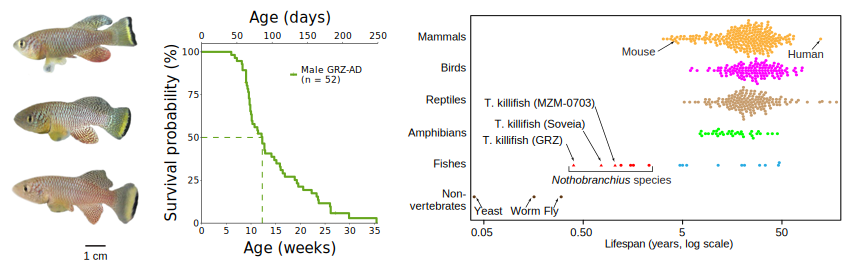
\includegraphics[width=0.95\textwidth]{output_files/figures/pdf/intro-turquoise-killifish}
\begin{subfigure}{0em}
\phantomsubcaption{}
\label{fig:intro-killifish-photos}
\end{subfigure}
\begin{subfigure}{0em}
\phantomsubcaption{}
\label{fig:intro-killifish-life-cycle}
\end{subfigure}
\begin{subfigure}{0em}
\phantomsubcaption{}
\label{fig:intro-killifish-lifespan}
\end{subfigure}
\begin{subfigure}{0em}
\phantomsubcaption{}
\label{fig:intro-killifish-comparison}
\end{subfigure}
\Caption{The turquoise killifish (\nfu) as a model for vertebrate ageing}{(A) Photographs of adult male yellow-tailed turquoise killifish.
(B) Life cycle of the turquoise killifish in its natural environment, showing hatching and breeding during the rainy season and embryo survival in diapause during the dry season.
(C) Example lifespan curve of short-lived GRZ-AD turquoise-killifish males, hatched in December 2016, with a median lifespan of roughly 12 weeks.
(D) Comparison of turquoise-killifish maximum lifespan (red triangles) to other vertebrate species, demonstrating the extremely short lifespan of GRZ-strain \Nfu compared to other vertebrates. (A), (B) and (D) adapted from \parencite{valenzano2015genome}, Figure 1.}
\label{fig:intro-killifish}
\end{figure}

\fi

\begin{document}
\maketitle

%% ******************************** Front Matter ********************************
%% Dedication, abstracts, acknowledgements etc. - do this last.

\frontmatter
% ******************************* Thesis Dedication ********************************
{
\cleardoublepage
\setsinglecolumn
\vspace*{0.2\textheight}
\thispagestyle{empty}
\begin{flushright}\doublespacing\textit{
    {\LARGE Cre\'{e}r, c'est recombiner.}\\
    -- Fran\c{c}ois Jacob \citep{hsu2015pathogen}}
\end{flushright}
}

% ************************** Thesis Abstract *****************************
{
\cleardoublepage
\setsinglecolumn
\chapter*{\centering \LARGE Kurzzusammenfassung}
\thispagestyle{empty}
Alternde Menschen zeigen einen stetigen R\"uckgang der adaptiven Immunfunktion, mit wichtigen Auswirkungen auf Gesundheit und Lebensdauer. Systemische Ver\"anderungen, die in der Struktur und Diversit\"at des Antik\"orperrepertoires mit dem Alter beobachtet werden, spielen eine wichtige Rolle in diesem immunoseneszenten Ph\"anotypen; die relativ lange Lebensdauer der meisten Wirbeltier-Modellorganismen macht eine gr\"undliche Untersuchung des alternden Immunrepertoires jedoch schwierig. Als nat\"urlich kurzlebiges Wirbeltier bietet der T\"urkise Prachtgrundk\"arpfling (\textit{Nothobranchius furzeri}) eine aufregende neue Gelegenheit, die Alterung des adaptiven Immunsystems im Allgemeinen und des Antik\"orperrepertoires im Besonderen zu untersuchen.

In dieser Arbeit habe ich eine Kombination aus bestehenden genomischen Assemblierungen und neu generierten Sequenzierungsdaten verwendet, um den Immunoglobulin-H-Ketten-Locus des T\"urkisen Prachtgrundk\"arpflings zusammenzusetzen, zu charakterisieren und mit Loci eng verwandter Arten zu vergleichen. Dies zeigt eine dynamische Locus-Entwicklung mit sich wiederholenden Duplizierungen und Verlusten des spezialisierten mukosalen Isotypen \textit{IGHZ}. Diese Ergebnisse unterst\"utzen eine hohe Evolutionsrate der Immunoglobulin-H-Ketten-Loci in den Teleostei und bilden eine solide Grundlage f\"ur die Forschung der vergleichenden evolution\"aren Immunologie in Zahnk\"arpflingen.

Nachdem ich die Immunoglobulin-H-Ketten-Locus-Sequenz in \textit{N. furzeri} charakterisiert hatte, nutzte ich sie, um Immunoglobulin-Sequenzierung gezielt f\"ur diese Spezies zu etablieren, welche eine quantitative Analyse des Antik\"orperrepertoires erm\"oglicht. Die Anwendung dieses Protokolls auf Ganzk\"orper-Fischproben ergab komplexe und individualisierte Antik\"orperrepertoires, die in der intraindividuellen Diversit\"at mit dem Alter rasch abnehmen und in der interindividuellen Variabilit\"at zunehmen. Dies zeigt, dass die Antik\"orperrepertoires von T\"urkisen Prachtgrundk\"arpflingen, entsprechend ihrer kurzen Lebensdauer schnelle Alterungsprozesse aufweisen. Dieser altersbedingte Diversit\"atsverlust war besonders stark in Darmproben - ein Ph\"anomen, das mit der konstanten ausgepr\"agten Antigenexposition an Schleimhautoberfl\"achen zusammenh\"angen kann und bisher nicht in einem Wirbeltier-Modell untersucht wurde. Zusammenfassend etablieren diese Ergebnisse den T\"urkisen Prachtgrundk\"arpfling als neuartiges Modell f\"ur die Erforschung von Immunoseneszenz in Wirbeltieren und bilden die Grundlage f\"ur zuk\"unftige Analysen von und Interventionsstudien an adaptiver Immunalterung.
}

% ************************** Thesis Abstract *****************************
{
\cleardoublepage
\setsinglecolumn
\chapter*{\centering \LARGE Abstract}
\thispagestyle{empty}

Ageing individuals exhibit a pervasive decline in adaptive immune function, with important implications for health and lifespan. Systemic changes observed in the structure and diversity of antibody repertoires with age are thought to play an important role in this immunosenescent phenotype; however, the relatively long lifespan of most vertebrate model organisms makes thorough investigation of the ageing repertoire challenging. As a naturally short-lived vertebrate, the turquoise killifish (\nfu) offers an exciting new opportunity to study the ageing of the adaptive immune system in general and antibody repertoires in particular.

In this thesis, I used a combination of existing genomic assemblies and new sequencing data to assemble and characterise the immunoglobulin heavy chain (\igh{}) locus sequence in the turquoise killifish and compare it to those of closely related species, revealing a history of dynamic locus evolution and repeated duplication and loss of the specialised mucosal isotype \igh{Z}. The \Nfu locus itself lacks \igh{Z}, making it one of the few known teleost species not to possess this isotype. These results support a high rate of evolution in teleost \igh{} loci and set a strong foundation for the study of comparative evolutionary immunology in cyprionodontiform fishes.

Having characterised the \igh{} locus sequence in \Nfu, I used it to establish targeted immunoglobulin sequencing in this species, enabling quantitative interrogation of the antibody repertoire. Applying this protocol to whole-body killifish samples revealed complex and individualised antibody repertoires which decline rapidly in within-individual diversity and increase in between-individual variability with age, demonstrating that turquoise killifish exhibit a rapid repertoire-ageing phenotype in line with their short lifespans. This loss of diversity with age was particularly strong in isolated gut samples, a phenomenon that may be related to the constant strong antigenic exposure experienced at mucosal surfaces and has not been previously investigated in a vertebrate model. Taken together, these results establish the turquoise killifish as a novel model for vertebrate immunosenescence and lay the groundwork for future interrogation of -- and intervention in -- adaptive-immune ageing.
}

% ************************** Thesis Acknowledgements **************************
{
\cleardoublepage
\setsinglecolumn
\chapter*{\centering \LARGE Acknowledgements}
\thispagestyle{empty}

A doctoral thesis in the life sciences might have a single author, but almost always has a great many direct and indirect contributors. Mine is no exception, and so I have a number of people to thank.

First, my sincere thanks to Dario Valenzano, who welcomed me into his research group in 2014 and has always been an enthusiastic, attentive and understanding supervisor. None of the work in this thesis would have been possible without him, and I would be a far poorer scientist without his mentorship and support.

Many members of the Valenzano group have actively contributed to this thesis. Patrick Smith performed the microbiota-transfer studies that were the inspiration for the project in the first place and supervised and mentored me through my first and most difficult year. Joanna Dodzian generously bred and provided the fish cohorts I used for the pilot and ageing experiments in \Cref{chap:igseq}. Rongfeng (Ray) Cui performed the genome assembly that laid the foundation for the work in \Cref{chap:locus} and provided a great deal of advice on both experimental procedures and computational analysis. My student supervisees, Linda Zirden, Lena Schlautmann, Pascha Hokama, and Davina Patel all made essential contributions to developing and testing the turquoise-killifish immunoglobulin-sequencing protocol; you were all great. 

Our tireless and wonderful technician, Aleksandra Placzek, has been an essential part of the \igseq project in the lab and performed several of the library preps; many of my favourite parts of this thesis would not have been possible without her. Most recently, Michael Poeschla has joined the repertoire-sequencing team and helped prepare the libraries for the final \igseq experiment in \Cref{chap:igseq}; I look forward to seeing where he takes the project in the future. In additional to Dario and Michael, my fellow students David Willemsen, Jens Seidel, Miriam Popkes and Daniel Davila all helped proofread the manuscript for this thesis; Miriam, David and especially Jens also did the lion's share of the work translating my abstract into German. I am sincerely grateful to all of them, and to all other past and present members of the Valenzano lab, for their help, support, and enthusiasm, and for making the group such a pleasant and friendly place in which to work.

A number of external collaborators and other scholars also made vital contributions to this work. Kathrin Reichwald provided me with essential BAC clones and a substantial amount of important advice. John Beausang, Aleksandra Walczak, Thierry Mora and Susana Magadan helped me get started in the enormous and somewhat intimidating world of immune-repertoire analysis, and Aleksandra in particular has repeatedly provided invaluable advice, introductions and insight. Jason Vander Heiden has tirelessly answered my many questions about the Immcantation pipeline and even made some changes to it at my request, while Quentin Marcou has been an invaluable help in getting to grips with his fantastic software \program{IGoR}. Tsimafei Padvitski and Davi Silva generously provided additional proofreading. Many other researchers have responded to my pestering emails, given advice where I needed it, and generally been friendly, welcoming and generous with their time. I am grateful to you all.

The co-ordination team of the Cologne Graduate School of Ageing Research has consistently been amazing, and I have repeatedly been impressed at the depth of their dedication, sympathy and willingness to help us students with all our big and little problems. My sincere thanks to Daniela Morick, Doris Birker and Jenny Ostermann for all their help and support. Thanks also to Ruth Willmott, for her invaluable soft-skills and careers coaching; Jorge Boucas, Franzi Metge, Daniel Rosskopp and the rest of the bioinformatics core facility for their patient help and advice; and all the other people I have unaccountably failed to mention here whose assistence, friendship and support I have relied on throughout this lengthly process.

My family, of course, have been a constant source of love and support. Mum, Dad, Anna, thank you for everything. I love you. My love and thanks also to the rest of my family, especially Ron and Julie, for their enduring support and belief in me and my research. 

Finally, my deepest and sincerest thanks to Simon Woolf, without whom this entire long adventure would have been a great deal more difficult and a great deal less fun.
}

%%%%%%%%%%%%%%%%%%%%%%%%%%%%%%%%%%%%%%%%%%%%%%%%%%%%%%%%%%%%%%%%%%%%%%%%%%%%%%%
%% STANDARD ENGLISH ABBREVIATIONS
%%%%%%%%%%%%%%%%%%%%%%%%%%%%%%%%%%%%%%%%%%%%%%%%%%%%%%%%%%%%%%%%%%%%%%%%%%%%%%%

\newabbreviation{c}{c.}{\textit{circa} (approximately)}
\newabbreviation{etc}{etc.}{\textit{et cetera} (and so on)}
\newabbreviation{vs}{vs}{\textit{versus} (against, compared to)}
\newabbreviation{e.g.}{e.g.}{\textit{exempli gratia} (for example)}
\newabbreviation{i.e.}{i.e.}{\textit{id est} (that is to say)}
\newabbreviation{et al.}{et al.}{\textit{et alia} (and others)}
\newabbreviation{ID}{ID}{identity}
\newabbreviation{aka}{a.k.a.}{also known as}
\newabbreviation{pm}{$\pm$}{plus or minus}
\newabbreviation{hash}{$\#$}{number of}

%%%%%%%%%%%%%%%%%%%%%%%%%%%%%%%%%%%%%%%%%%%%%%%%%%%%%%%%%%%%%%%%%%%%%%%%%%%%%%%
%% UNITS
%%%%%%%%%%%%%%%%%%%%%%%%%%%%%%%%%%%%%%%%%%%%%%%%%%%%%%%%%%%%%%%%%%%%%%%%%%%%%%%

% Volume
\newabbreviation{l}{L}{litre(s)}
\newabbreviation{ul}{\textmu{}l}{microlitre(s)}
\newabbreviation{ml}{ml}{millilitre(s)}

% Mass
\newabbreviation{gram}{g}{gram(s)}
\newabbreviation{ng}{ng}{nanogram(s)}

% Time
\newabbreviation{s}{s}{second(s)}
\newabbreviation{min}{min}{minute(s)}
\newabbreviation{h}{h}{hour(s)}
\newabbreviation{Mya}{Mya}{million years ago}

% Temperature
\newabbreviation{degC}{\textdegree{}C}{degrees Celsius}

% Concentration
\newabbreviation{M}{M}{molar concentration (\cu{\mole\per\liter}{}{})}
\newabbreviation{times}{$\times$}{multiples (e.g. of standard concentration)}
\newabbreviation{uM}{\textmu{}M}{micromolar concentration (\cu{\micro\mole\per\liter}{}{})}
\newabbreviation{mM}{mM}{millimolar concentration (\cu{\milli\mole\per\liter}{}{})}
\newabbreviation{nM}{nM}{nanomolar concentration (\cu{\nano\mole\per\liter}{}{})}

% Quantity
\newabbreviation{mol}{mol}{mole(s) (unit of amount of substance)}
\newabbreviation{nmol}{nmol}{nanomole(s)}
\newabbreviation{umol}{\textmu{}mol}{micromole(s)}
\newabbreviation{mmol}{mmol}{millimole(s)}

% Proportion
\newabbreviation{pc}{\%}{percent}
\newabbreviation{wv}{w/v}{weight/volume}
\newabbreviation{vv}{v/v}{volume/volume}

% Other
\newabbreviation{degrees}{\textdegree{}}{degrees (angle)}
\newabbreviation[sort=g]{g}{$g$}{relative centrifugal force}
\newabbreviation{U}{U}{unit(s) of enzyme activity}
\newabbreviation{bit}{bit}{binary digit (unit of information)}
\newabbreviation{nat}{nat}{natural unit (unit of information)}


%%%%%%%%%%%%%%%%%%%%%%%%%%%%%%%%%%%%%%%%%%%%%%%%%%%%%%%%%%%%%%%%%%%%%%%%%%%%%%%
%% MOLECULES AND MIXTURES
%%%%%%%%%%%%%%%%%%%%%%%%%%%%%%%%%%%%%%%%%%%%%%%%%%%%%%%%%%%%%%%%%%%%%%%%%%%%%%%

% Molecules
\newabbreviation{RNA}{RNA}{ribonucleic acid}
\newabbreviation{DNA}{DNA}{deoxyribonucleic acid}
\newabbreviation{PEG}{PEG}{polyethylene glycol}
%\newabbreviation[sort=H2O]{H2O}{H\textsubscript{2}O}{water}
\newabbreviation{dNTP}{dNTP}{deoxyribonucleoside triphosphate mix (dATP, dGTP, dCTP and dTTP)}
\newabbreviation{dATP}{dATP}{deoxyadenosine triphosphate}
\newabbreviation{dGTP}{dGTP}{deoxyguanosine triphosphate}
\newabbreviation{dCTP}{dCTP}{deoxycytidine triphosphate}
\newabbreviation{dTTP}{dTTP}{deoxythymidine triphosphate}
\newabbreviation{DTT}{DTT}{dithiothreitol (reducing agent)}
\newabbreviation{mRNA}{mRNA}{messenger RNA}
\newabbreviation{cDNA}{cDNA}{complementary DNA}
\newabbreviation{TRB}{TRB}{T-cell receptor beta}
\newabbreviation{EDTA}{EDTA}{ethylenediaminetetraacetic acid}

% Enzymes
\newabbreviation{UDG}{UDG}{uracil-DNA glycosylase}
\newabbreviation{TdT}{TdT}{terminal dideoxy transferase}


% Buffers
\newabbreviation{TET}{TET}{Tris:EDTA:Tween (buffer)}
\newabbreviation{iSB}{iSB}{incomplete SeraBind (buffer)}
\newabbreviation{EB}{EB}{elution buffer}

% Other
\newabbreviation{PCI}{PCI}{phenol:chloroform:isoamyl alcohol mixture}
\newabbreviation{LB}{LB}{lysogeny broth}


%%%%%%%%%%%%%%%%%%%%%%%%%%%%%%%%%%%%%%%%%%%%%%%%%%%%%%%%%%%%%%%%%%%%%%%%%%%%%%%
%% TECHNIQUES
%%%%%%%%%%%%%%%%%%%%%%%%%%%%%%%%%%%%%%%%%%%%%%%%%%%%%%%%%%%%%%%%%%%%%%%%%%%%%%%

\newabbreviation{PCR}{PCR}{polymerase chain reaction}
\newabbreviation{HiFi}{HiFi}{high-fidelity (PCR)}
\newabbreviation{IgSeq}{IgSeq}{immunoglobulin sequencing}
\newabbreviation{SPRI}{SPRI}{solid-phase reversible immobilisation}
\newabbreviation{BR}{BR}{broad-range (Qubit assay)}
\newabbreviation{HS}{HS}{high-sensitivity (Qubit assay)}
\newabbreviation{RDI}{RDI}{Repertoire Dissimilarity Index}


%%%%%%%%%%%%%%%%%%%%%%%%%%%%%%%%%%%%%%%%%%%%%%%%%%%%%%%%%%%%%%%%%%%%%%%%%%%%%%%
%% SCIENTIFIC TERMINOLOGY 
%%%%%%%%%%%%%%%%%%%%%%%%%%%%%%%%%%%%%%%%%%%%%%%%%%%%%%%%%%%%%%%%%%%%%%%%%%%%%%%

% Genetics
\newabbreviation{bp}{bp}{base pair(s)}
\newabbreviation{BAC}{BAC}{bacterial artificial chromosome}
\newabbreviation{TSA}{TSA}{template-switch adapter}
\newabbreviation{PhiX}{PhiX}{PhiX174 bacteriophage genome}
\newabbreviation{GSP}{GSP}{gene-specific primer (for reverse transcription)}
\newabbreviation{kb}{kb}{kilobase(s)}
\newabbreviation{UTR}{UTR}{untranslated region}
\newabbreviation{NHEJ}{NHEJ}{non-homologous end-joining}
\newabbreviation{chr}{chr}{chromosome}
\newabbreviation{scf}{scf}{scaffold (genome assembly)}
\newabbreviation{oligo}{oligo}{oligonucleotide}
\newabbreviation{prep}{prep}{preparation}
\newabbreviation{DSB}{DSB}{double-strand break}
\newabbreviation{NT}{NT}{nucleotide(s)}
\newabbreviation{AA}{AA}{amino acid(s)}
\newabbreviation{nt}{nt}{nucleotide(s)}

% Immunology
\newabbreviation{VH}{VH}{heavy-chain variable (gene segment)}
\newabbreviation{DH}{DH}{heavy-chain diversity (gene segment)}
\newabbreviation{JH}{JH}{heavy-chain joining (gene segment)}
\newabbreviation{RAG}{RAG}{recombination-activating gene}
\newabbreviation{RSS}{RSS}{recombination signal sequence}
\newabbreviation{BCR}{BCR}{B-cell receptor}
\newabbreviation{IGH}{IGH}{immunoglobulin heavy chain}
\newabbreviation{IGL}{IGL}{immunoglobulin light chain}
\newabbreviation{CDR}{CDR}{complementarity-determining region}
\newabbreviation{FR}{FR}{framework region}
\newabbreviation{FWR}{FWR}{framework region}
\newabbreviation{TM}{TM}{transmembrane exon}
\newabbreviation{CH}{CH}{heavy-chain constant-region exon}
\newabbreviation{CM}{CM}{IGHM constant-region exon}
\newabbreviation{CD}{CD}{IGHD constant-region exon}
\newabbreviation{CZ}{CZ}{IGHZ constant-region exon}
\newabbreviation[sort=Cmu]{cm1}{\cm{}}{IGHM constant-region exon}
\newabbreviation[sort=Cdelta]{cd1}{\cd{}}{IGHD constant-region exon}
\newabbreviation[sort=Czeta]{cz1}{\cz{}}{IGHZ constant-region exon}
\newabbreviation{CSR}{CSR}{class-switch recombination}
\newabbreviation{IGHM}{IGHM}{Immunoglobulin M (isotype of IGH)}
\newabbreviation{IGHD}{IGHD}{Immunoglobulin D (isotype of IGH)}
\newabbreviation{IGHZ}{IGHZ}{Immunoglobulin Z (isotype of IGH)}
\newabbreviation{IGHT}{IGHT}{Immunoglobulin T (equivalent to IGHZ)}
\newabbreviation{IGHT/Z}{IGHT/Z}{Immunoglobulin T/Z (equivalent to IGHZ)}
\newabbreviation{IGHZ/T}{IGHZ/T}{Immunoglobulin Z/T (equivalent to IGHZ)}
\newabbreviation{SHM}{SHM}{somatic hypermutation}
\newabbreviation{AID}{AID}{activation-induced cytidine deaminase}
\newabbreviation{FDC}{FDC}{follicular dendritic cell}
\newabbreviation{GALT}{GALT}{gut-associated lymphoid tissue}
\newabbreviation{HSC}{HSC}{haematopoietic stem cell}
\newabbreviation{IGHM-S}{IGHM-S}{secretory IGHM}
\newabbreviation{IGHM-TM}{IGHM-TM}{transmembrane IGHM}
\newabbreviation{IGHD-TM}{IGHD-TM}{transmembrane IGHD}

% Bioinformatics/statistics
\newabbreviation{HSP}{HSP}{high-scoring segment pair (\program{BLAST})}
\newabbreviation{E-value}{E-value}{Expect value (\program{BLAST})}
\newabbreviation{HMM}{HMM}{Hidden Markov Model}
\newabbreviation{SA}{SA}{suffix array}
\newabbreviation{UMI}{UMI}{unique molecular identifier}
\newabbreviation{MIG}{MIG}{molecular identifier group}
\newabbreviation{GLM}{GLM}{generalised linear model}
\newabbreviation{RIN}{RIN}{RNA integrity number}
\newabbreviation{EMBOSS}{EMBOSS}{European Molecular Biology Open Software Suite}
\newabbreviation{RNA-seq}{RNA-seq}{RNA sequencing}
\newabbreviation{PCoA}{PCoA}{principal co-ordinate analysis}
\newabbreviation{KWT}{KWT}{Kruskal-Wallis test}

%%%%%%%%%%%%%%%%%%%%%%%%%%%%%%%%%%%%%%%%%%%%%%%%%%%%%%%%%%%%%%%%%%%%%%%%%%%%%%%
%% TAXA
%%%%%%%%%%%%%%%%%%%%%%%%%%%%%%%%%%%%%%%%%%%%%%%%%%%%%%%%%%%%%%%%%%%%%%%%%%%%%%%

% Species
\newabbreviation[sort=P. playfairii]{ppl}{\textit{P. playfairii}}{\textit{Pachypanchax playfairii}}
\newabbreviation[sort=O. latipes]{ola}{\textit{O. latipes}}{\textit{Oryzias latipes}}
\newabbreviation[sort=A. australe]{aau}{\textit{A. australe}}{\textit{Aphyosemion australe}}
\newabbreviation[sort=N. orthonotus]{nor}{\textit{N. orthonotus}}{\textit{Nothobranchius orthonotus}}
\newabbreviation[sort=A. limnaeus]{ali}{\textit{A. limnaeus}}{\textit{Austrofundulus limnaeus}}
\newabbreviation[sort=P. formosa]{pfo}{\textit{P. formosa}}{\textit{Poecilia formosa}}
\newabbreviation[sort=P. reticulata]{pfo}{\textit{P. reticulata}}{\textit{Poecilia reticulata}}
\newabbreviation[sort=F. heteroclitus]{fhe}{\textit{F. heteroclitus}}{\textit{Fundulus heteroclitus}}
\newabbreviation[sort=K. marmoratus]{kma}{\textit{K. marmoratus}}{\textit{Kryptolebias marmoratus}}
\newabbreviation[sort=C. toddi]{cto}{\textit{C. toddi}}{\textit{Callopanchax toddi}}
\newabbreviation[sort=C. variegatus]{cva}{\textit{C. variegatus}}{\textit{Cyprinodon variegatus}}
\newabbreviation[sort=N. furzeri]{nfu}{\textit{N. furzeri}}{\nfu}
\newabbreviation[sort=E. coli]{ecoli}{\textit{E. coli}}{\textit{Escherichia coli}}
\newabbreviation[sort=X. maculatus]{xma}{\Xma}{\xma}
\newabbreviation[sort=H. sapiens]{hsa}{\textit{H. sapiens}}{\textit{Homo sapiens}}

% Strains
\newabbreviation{GRZ}{GRZ}{strain of \Nfu (from Gonarezhou National Park, Zimbabwe)}
\newabbreviation{GRZ-AD}{GRZ-AD}{substrain of GRZ}
\newabbreviation{bellemans}{GRZ-Bellemans}{substrain of GRZ}

%%%%%%%%%%%%%%%%%%%%%%%%%%%%%%%%%%%%%%%%%%%%%%%%%%%%%%%%%%%%%%%%%%%%%%%%%%%%%%%
%% OTHER
%%%%%%%%%%%%%%%%%%%%%%%%%%%%%%%%%%%%%%%%%%%%%%%%%%%%%%%%%%%%%%%%%%%%%%%%%%%%%%%

% Parameters
\newabbreviation[sort=T_a]{ta}{$\boldsymbol{T_a}$}{annealing temperature (PCR)}
\newabbreviation[sort=t_{ext}]{t_ext}{$\boldsymbol{t_{ext}}$}{extension time (PCR)}
\newabbreviation[sort=n_c]{n_c}{$\boldsymbol{n_c}$}{cycle number (PCR)}

% Locations
\newabbreviation{FLI}{FLI}{Leibniz Institute on Aging – Fritz Lipmann Institute (Jena, Germany)}

%% *********************** Adding TOC and List of Figures ***********************
%%%
\renewcommand{\baselinestretch}{0.9}%
\tableofcontents%
\renewcommand{\baselinestretch}{1.0}%
%%
\listoffigures
%%
\listoftables
%%
\setlength{\glslistdottedwidth}{4cm}
\setglossarystyle{listdotted}
\printglossary[title={List of abbreviations},nonumberlist=true,nogroupskip=true]

%% ******************************** Main Matter *********************************
\mainmatter\onehalfspacing
%
\chapter{Introduction}
\label{chap:intro}
\onehalfspacing

\pagebreak

\section{Overview}
\label{sec:intro_overview}

All organisms exist in a state of intense competition for resources. For many organisms, among the most dangerous competitors are parasites, which attempt to colonise the host's own body and co-opt its internal resources and systems to their own advantage. The evolutionary arms race between parasites and hosts is ancient, and has led to the development of a stunning variety of complex offensive and defensive adaptations on each side \parencite{jack2015evolution}. Immunology has therefore had a profound effect on evolution.

One of the most complex and sophisticated systems developed as part of this ancient host/parasite conflict is the vertebrate adaptive immune system. By dynamically recombining their own DNA within specialised lymphocyte cells (\Cref{sec:intro_immunity_primary}), jawed vertebrates are capable of producing an almost unlimited variety of different \textit{de novo} antigen-receptor proteins, and hence of responding effectively to entirely novel immune threats \parencite{jack2015evolution}. In addition, by producing long-lived memory cells in response to antigenic stimulation, the adaptive immune system can retain the ability to respond to recurrent threats years or even decades after they were first encountered by an individual \parencite{kurosaki2015memory} (\Cref{sec:intro_affinity_maturation}). This combination of dynamic adaptability to novel immune threats and persistent immune memory enables vertebrates to progressively improve their protection against predictable aspects of their immune environment \parencite{mayer2018memory}, while also coping effectively with the rapid evolution of bacterial and viral pathogens.

Among the different branches of vertebrate adaptive immunity, the B-cell-mediated humoral immune system is unique in both the breadth of antigenic compounds it can respond to and its ability to produce secreted antigen-receptor proteins capable of acting independently of the cells that produced them. Whereas the T-lymphocytes of the cellular adaptive immune system can respond only to processed peptide antigens expressed on the surface of antigen-presenting cells, the antibodies produced by B-lymphocytes (\Cref{sec:intro_antibody_structure}) are capable of responding to a much wider variety of organic molecules, including proteins, carbohydrates, nucleic acids, and lipids \parencite{sompayrac2019immune}. Secreted antibodies in serum and mucosal secretions play a number of essential roles in vertebrate immunity, including opsonisation (recruitment of phagocytic cells), activation of complement, and inactivation and aggregation of antigens and pathogens \parencite{schroeder2010immunoglobulins}, while membrane-bound antibodies (also known as B-cell receptors or BCRs \parencite{bengten2015fishantibodies}) orchestrate B-cell development and response to antigen exposure. An effective humoral immune system is essential to immune function in vertebrates, and mutations that impair antibody production can cause severe immunodeficiency syndromes in humans \parencite{vanzelm2006cd19}.

Despite all its sophistication, however, the functionality of the vertebrate adaptive immune system declines dramatically with age, leaving older individuals increasingly vulnerable to infectious disease (\Cref{sec:intro_immunosenescence}). In humans and other species, the decline in immune functionality with age manifests as a dramatic increase in deaths from infection in older people, as well as increasing levels of infection-associated morbidity and a decline in the effectiveness of pro-immune interventions such as vaccination \parencite{sambhara2009vaccination}. The molecular and physiological changes underlying this immunosenescent phenotype are wide-ranging, implicating many different parts of the immune system; however, one particularly important contributor is the systemic decline in the effectiveness of the adaptive immune system. For the humoral immune system, well-established immunosenescent phenotypes include a fall in \naive B-cell output from the bone marrow, reduced antibody quality, impaired affinity maturation, and a serious decline in the ability to mount an effective antibody response to vaccination (\Cref{sec:intro_immunosenescence}).

While much has been discovered about the cellular and physiological changes that take place in the humoral adaptive immune system with age in some species, particularly humans and mice, much less is known about how these changes translate to alterations in the high-level diversity, clonal makeup, and other structural aspects of the overall antibody repertoire in older individuals. Such a high-level systemic approach to antibody diversity could potentially reveal a great deal about how ageing and other processes affect adaptive immune functionality in an organism. Specialised, high-throughput, quantitative approaches \parencite{georgiou2014promise} have been used to assess the structure, diversity and health of adaptive immune repertoires in various contexts, including development, disease, and ageing; in the latter case, this pre-existing work has confirmed a loss of antibody-repertoire diversity with age, accompanied by impaired primary and clonal B-cell selection, an increase in memory-cell clonal expansions, and an increase in between-individual variablity in the repertoires of older individuals (\Cref{sec:intro_immunosenescence}). However, much remains to be discovered about the temporal and spatial progression of repertoire ageing, the effect of anti-ageing interventions, and the comparative effects of ageing on repertoires from species other than humans and mice.

When it comes to investigating the ageing of vertebrate-specific adaptations like the adaptive immune system, research is made more difficult by a relative lack of well-suited model organisms. Most established short-lived model organisms used in ageing research (e.g. yeast, nematode worms, or fruit flies) are not vertebrates, while most established vertebrate models (e.g. zebrafish or \species{Xenopus}{laevis}) were selected for properties other than their lifespan (such as rapid development) and are too long-lived for use as ageing models in many contexts \parencite{gerhard2002zebrafish,bowler1977longevity}. Even mice, the most widely-used vertebrate model organisms for both ageing and other biomedical applications, have a median lifespan of several years in most commonly-used laboratory strains \parencite{yuan2009aging}, making many ageing studies prohibitively expensive. In this context, the recent emergence of the turquoise killifish (\nfu), the shortest-lived vertebrate species currently bred in captivity, as a model organism for ageing research (\Cref{sec:intro_killifish}) represents a highly promising development for the study of adaptive immunosenescence, providing the opportunity to rapidly investigate the ageing of the antibody repertoire over the entire lifespan of an organism, in different organs, and in response to known anti-ageing interventions. 

In this thesis, therefore, I establish the turquoise killifish as a model for the study of comparative immunology and humoral adaptive immunosenescence. Using a combination of existing genomic assemblies and new sequence data, I assembled and characterised the immunoglobulin heavy chain (\igh{}) gene locus of the turquoise killifish and compared it to other newly-assembled loci from closely-related species, revealing a group of complex and rapidly-evolving loci with a number of surprisingly ideosyncratic features (\Cref{chap:locus}). Using the sequences from this newly-characterised locus, I established the first working immunoglobulin-sequencing protocol in this species, which I used to investigate the diversity and complexity of heavy-chain immune repertoires in adult killifish and how this diversity changes with age in the whole body and the gut (\Cref{chap:igseq}). The results of these investigations demonstrate that the turquoise killifish possesses a complex, diverse and individualised antibody repertoire, which undergoes a rapid decline in within-individual diversity and increase in between-individual variability with age. This phenomenon is particularly strong in the gut mucosal repertoire, likely as a result of the much greater relative prelavence of large, antigen-experienced clones and the intense antigen exposure of mucosal B-cell populations. Taken together, these results demonstrate the value of the turquoise killifish as an emerging model system in vertebrate immunology.

\section{The humoral adaptive immune system in jawed vertebrates}
\label{sec:intro_antibodies}

\subsection{Antibody structure and function}
\label{sec:intro_antibody_structure}

The lineage of lymphocytic white blood cells known as B-cells is ancient, with its origins predating any modern jawed-vertebrate lineage \parencite{boehm2011design,kasahara2015vlr}. In modern jawed vertebrates, B-lymphocytes are responsible for the production, diversification and secretion of the antigen-receptor proteins known as antibodies \parencite{mix2006immunoglobulins,schroeder2010immunoglobulins}, as well as diverse other roles that vary between taxa \parencite{sunyer2013fishing}. In almost all species examined to date, antibodies share a common, and highly distinctive, tetrameric structure (\Cref{fig:intro-antibody-structure-schematic}), with two identical immunoglobulin heavy chains (IGH) and two light chains (IGL) linked by disulfide bonds into a roughly Y-shaped configuration \parencite{mix2006immunoglobulins,schroeder2010immunoglobulins}. The sequence and structure of these chains, and the corresponding regions of their underlying gene loci, is divided into an N-terminal (5') variable region and a C-terminal (3') constant region \parencite{mix2006immunoglobulins} (\Cref{fig:intro-antibody-structure-schematic}); together, the variable regions of each light/heavy-chain pair determines the antigen-binding specificity of the antibody, while the constant regions, particularly that of the heavy chain, determine its structure, functional properties, and interactions with the rest of the immune system \parencite{mix2006immunoglobulins,schroeder2010immunoglobulins}. Unsurprisingly, the sequence diversity of the constant region is far lower than that of the variable region, with most species expressing only a few distinct constant-region classes (or \textit{isotypes}) but an almost unlimited variety of variable-region sequences (or \textit{ideotypes}).

As members of the immunoglobulin superfamily of proteins, the tertiary structure of antibody chains consists primarily of a species of immunoglobulin-fold domains; most light chains consist of two such domains, while the number in heavy chains varies substantially with isotype \parencite{schroeder2010immunoglobulins}. In both heavy and light chains, the most N-terminal immunoglobulin fold comprises the variable region, while the rest make up the constant region (\Cref{fig:intro-antibody-structure-schematic}); in some taxa (but not in teleost fishes), one of the constant-region immunoglobulin folds is replaced with a flexible hinge domain in some isotypes to increase the flexibility of the heavy chain \parencite{schroeder2010immunoglobulins}. The three loops of the protein chain facing the antigen-binding site are labelled H1, H2 and H3 in the heavy chain and L1, L2 and L3 in the light chain (\Cref{fig:intro-antibody-structure-loops}) \parencite{shirai1999h3} and are principally responsible for determining the antigen-binding specificity of the antibody; their corresponding gene regions are known as complementarity-determining regions (CDRs) and are the main focus of sequence variability among ideotypes, while the other parts of the antibody sequence are known as framework regions (FRs or FWRs) and exhibit less variability \parencite{schroeder2010immunoglobulins}.

Most antibody isotypes can be expressed in secreted or membrane-bound form; in the latter case they are also known as B-cell receptors (BCRs) \parencite{bengten2015fishantibodies}. The choice between secreted and membrane-bound forms of an antibody is usually made through alternative splicing \parencite{bengten2015fishantibodies,mashoof2016immunoglobulins}; typically, the transmembrane domain and cytosolic tail of the BCR are expressed via two additional exons (TM1 and TM2). Other constant-region exons are referred to collectively as CH exons, and are numbered by their occurence in the protein chain from the variable region to the C-terminus. In secreted antibodies, the standard four-chain configuration described above is known as an antibody monomer \parencite{mix2006immunoglobulins}, while multiple four-chain antibodies bound together are referred to by the number of four-chain monomer subunits they contain: dimers for two connected subunits, tetramers for four, etc. \parencite{mix2006immunoglobulins,schroeder2010immunoglobulins} (\Cref{fig:intro-antibody-structure-multimers}). These multimeric antibody supercomplexes have increased overall avidity for antigen and so can respond more strongly to low levels of low-specificity antigen \parencite{mix2006immunoglobulins}; they can be bound together by covalent disulfide bonds between subunits \parencite{schroeder2010immunoglobulins} or, more rarely, by noncovalent intermolecular interactions \parencite{zhang2010igtgut}.

Of the two types of chain comprising the antibody protein, the heavy chain has by far the larger effect on antigen specificity \parencite{shirai1999h3}, as well as determining the antibody's effector function  \parencite{schroeder2010immunoglobulins}; this thesis therefore focuses exclusively on the heavy chain. The number and variety of antibody heavy-chain classes available to B-cells in an organism, and the mechanism by which the isotype of an antibody is determined, vary substantially by species; in tetrapods, the isotype of the antibodies produced by a given B-cell can be modified by a specialised class-switch recombination (CSR) process which is absent in teleost fishes \parencite{senger2015switching}. Different isotypes vary in their length, flexibility, multimerisation behaviour, and effector functions \parencite{schroeder2010immunoglobulins,senger2015switching}. In teleost fishes, three constant-region classes have been observed to date \parencite{bengten2015fishantibodies,mashoof2016immunoglobulins,fillatreau2013astonishing}:

\begin{itemize}
\item \textbf{Immunoglobulin M} (\igh{M}) was the first \igh{} isotype to be identified in teleosts \parencite{fillatreau2013astonishing}, and is homologous to the isotype of the same name found in mammals and other jawed vertebrates \parencite{mashoof2016immunoglobulins}. It is expressed in both secreted and transmembrane form \parencite{fillatreau2013astonishing}; in most teleosts, the transcript of the secreted form comprises four CH exons (\cm{1-4}), while the transmembrane form comprises three CH exons and two TM exons \parencite{bengten2015fishantibodies,fillatreau2013astonishing}. In contrast to mammals, in which secreted \igh{M} is primarily found as a pentamer, in teleosts it is typically found as a tetramer \parencite{fillatreau2013astonishing} connected by disulfide bonds between heavy chains \parencite{mashoof2016immunoglobulins}. In those fish species which have been tested, secreted \igh{M} is the main form of antibody found in serum \parencite{bengten2015fishantibodies,mashoof2016immunoglobulins,fillatreau2013astonishing}.

\item Like \igh{M}, \textbf{immunoglobulin D} (\igh{D}) is a primitive isoform present in most lineages of jawed vertebrates \parencite{mashoof2016immunoglobulins}, including teleost fishes. The size and structure of \igh{D} varies dramatically between teleost species, with the number of CH exons varying more than twofold, from roughly seven (\cd{1-7}) in some species to seventeen in zebrafish \parencite{mashoof2016immunoglobulins,fillatreau2013astonishing}. All teleost \igh{D} transcripts to date have possessed a chimeric \cm{1} exon from \igh{M}, a configuration almost unknown in mammals \parencite{mashoof2016immunoglobulins,fillatreau2013astonishing}; teleost \igh{D} also lacks the flexible hinge region present in mammalian \igh{D} \parencite{fillatreau2013astonishing}. A minority of teleost species are known to possess secretory forms of \igh{D}, though the mechanism of producing them varies: in channel catfish, one dedicated sublocus has a dedicated \igh{D} secretory exon in place of the transmembrane exons \parencite{bengten2006catfish} (\Cref{fig:intro-teleost-loci-complex}), while in rainbow trout (and possibly some other species like Atlantic salmon and cod) a run-on event at the end of \cd{7} results in the production of a secretory tail in a manner similar to secretory \igh{Z} \parencite{ramirezgomez2012secretoryigd}. In other species, only transmembrane isoforms have been observed. In teleosts as in mammals, transmembrane \igh{D} is usually co-expressed with \igh{M}; however, its role in the adaptive immune system remains unclear \parencite{mashoof2016immunoglobulins}. % 

\item Unlike \igh{M} and \igh{D}, \textbf{immunoglobulin Z} (\igh{Z}, also known as \igh{T}, \igh{Z/T} and \igh{Z/T}) is unique to teleost fishes \parencite{fillatreau2013astonishing}. Also unlike \igh{M} and \igh{D}, \igh{Z} is not found universally among teleost loci -- of those \igh{} loci characterised to date, \igh{Z} is missing in those of medaka and channel catfish (\Cref{fig:intro-teleost-loci-complex})  \parencite{fillatreau2013astonishing,magadan2011medaka}, having apparently been lost independently in these species (\Cref{fig:intro-teleost-loci-complex}). In those species in which it is present, \igh{Z} appears to act as a specialised mucosal antibody class, with elevated levels observed in mucosal secretions compared to serum \parencite{zhang2010igtgut,fillatreau2013astonishing,xu2013igtskin}. Unlike \igh{M}, secretory \igh{Z} in serum is predominantly monomeric, while in mucosal secretions it is found primarily as a tetramer held together by noncovalent intermolecular bonds between heavy chains \parencite{zhang2010igtgut}. In most species, \igh{Z} comprises four CH exons (\cz{1-4}) and two TM exons \parencite{mashoof2016immunoglobulins}, though some species have fewer -- for example, stickleback \igh{Z} has only three CH exons \parencite{bao2010stickleback,gambondeza2011stickleback}, while fugu \igh{Z} has only two \parencite{fillatreau2013astonishing,savan2005fugu}.
\end{itemize}

\begin{figure}
\centering
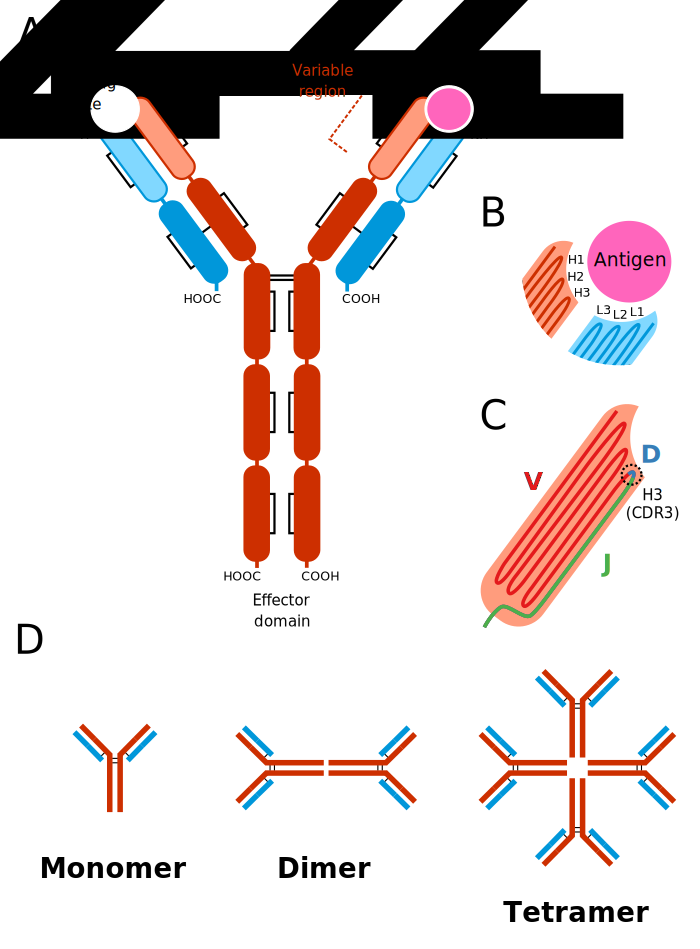
\includegraphics[width=0.9\textwidth]{output_files/figures/pdf/intro-antibody-structure}
\begin{subfigure}{0em}
\phantomsubcaption{}
\label{fig:intro-antibody-structure-schematic}
\end{subfigure}
\begin{subfigure}{0em}
\phantomsubcaption{}
\label{fig:intro-antibody-structure-loops}
\end{subfigure}
\begin{subfigure}{0em}
\phantomsubcaption{}
\label{fig:intro-antibody-structure-vdj}
\end{subfigure}
\begin{subfigure}{0em}
\phantomsubcaption{}
\label{fig:intro-antibody-structure-multimers}
\end{subfigure}
\Caption{Antibody structure and function}{(A) Schematic of a hingeless secreted antibody monomer, with heavy chains depicted in red, light chains in blue, and bound antigen in pink. Immunoglobulin fold domains are depicted as rounded rectangles, with variable-region domains shown with light shading and constant-region domains with dark. Black lines indicate disulfide bonds. (B) Schematic close-up of an immunoglobulin antigen-binding site, indicating the six loop regions (H1-3 and L1-3) making up the antigen-binding region. (C) Schematic close-up of the heavy-chain variable region, indicating the regions corresponding to the variable, diversity and joining gene segments from the unrecombined \igh{} locus. Note the chimeric nature of the third antigen-binding loop (H3, marked), which is formed by parts of all three gene segments. (D) In the context of antibodies, ``monomer'' refers to a single four-chain antibody protein, while ``dimer'', ``tetramer'' etc. refer to multiple four-chain monomers linked together through covalent or noncovalent interactions.}
\label{fig:intro-antibody-structure}
\end{figure}

\subsection{Antibody sequence diversification and primary repertoire diversity}
\label{sec:intro_immunity_primary}

The immune environment encountered by a vertebrate organism contains an enormous number of different potential pathogenic threats, each of which has its own antigenic signatures and many of which are capable of evolving much more rapidly than the vertebrate host \parencite{jack2015evolution}. In order for the adaptive immune system to cope with this huge diversity of different threats, it must be able to produce antibodies with a correspondingly large diversity of different antigen specificities. The greater the potential diversity of antibody sequences available to the adaptive immune system, the greater its capacity to respond effectively to novel immune threats. In fact, the mechanisms employed by the vertebrate adaptive immune system to diversify its antigen receptors enable an almost unlimited diversity of potential antibody sequences, with a correspondingly vast array of potential antigen specificities \parencite{mora2016diversity}.

The mechanisms by which the adaptive immune system produces this diversity are dramatic, and rely on a highly unusual underlying gene structure \parencite{jung2006vdjr} and a very high level of cellular wastage \parencite{kogut2012bcells}. In the humoral immune system, antibody diversification takes place during B-cell development in the primary lymphoid organs (bone marrow in mammals, anterior kidney in teleosts \parencite{sunyer2013fishing}). Prior to this process, the native antibody loci in B-progenitor cells (and other cell types) are highly fragmented \parencite{jung2006vdjr}, with numerous variable-region sequence segments present in series on the chromosome upstream of the constant-region exons. In the heavy chain locus, these variable-region gene segments can be divided into three categories:

\begin{itemize}
\item \textbf{Variable (\vh) segments} are the longest class of gene segment, at roughly \bp{300} in length \parencite{lefranc2003vnumbering}. Each \vh segment codes for the majority of the variable region of an antibody, including the entirety of the first three framework regions (FWR1-3) and the first two complementarity-determining regions (CDR1-2) as well as the 5' part of CDR3 \parencite{schroeder2010immunoglobulins,jung2006vdjr} (\Cref{fig:intro-antibody-structure-vdj}). They are therefore highly structured, and include several highly-conserved positions present in virtually all functional V-segments in nearly all species, including two conserved cysteine residues (which give rise to an intra-domain disulfide bond) and a conserved tryptophan residue following CDR1 \parencite{lefranc2003vnumbering}. Each V-segment is also associated with its own promoter sequence and 5'-UTR, as well as a 5'/C-terminal leader peptide between the translation start site and the start of the functional V-sequence.
\item \textbf{Diversity (\dh) segments} are the shortest class of segment, typically on the order of 10-\bp{20}, and are the least structured \parencite{ruiz1999humandj}. They form the middle part of CDR3 (\Cref{fig:intro-antibody-structure-vdj}) \parencite{schroeder2010immunoglobulins}.
\item \textbf{Joining (\jh) segments} are of intermediate length, typically 50-\bp{60} \parencite{ruiz1999humandj}. They form the 3'/C-terminal part of heavy chain CDR3 and the 5'/N-terminal part of FR4 (\Cref{fig:intro-antibody-structure-vdj}) \parencite{schroeder2010immunoglobulins}. Each J-segment is succeeded on the chromosome by a splice donor site \parencite{magadan2011medaka}, which is used to join the variable region of the antibody sequence to the constant region via RNA splicing following transcription of \igh{} mRNA (\Cref{fig:intro-vdjr-locus}iii). Like \vh segments, \jh segments can be identified from their conserved structure, particularly the conserved tryptophan residue marking the end of CDR3 \parencite{ruiz1999humandj}.
\end{itemize}

In the simplest ``translocon'' configuration of the \igh{} locus, blocks of repeated \vh, \dh and \jh segments are present in series on the chromosome in contiguous V-, D- and J-regions (\Cref{fig:intro-vdjr-locus}i) \parencite{schroeder2010immunoglobulins,jung2006vdjr}. During B-cell development, a single \vh, \dh and \jh segment are selected from these segment blocks, and the intervening genomic regions are permanently excised from the genome to produce a single, contiguous VDJ sequence coding for the complete variable region of an antibody (\Cref{fig:intro-vdjr-locus}ii). The mechanism by which this excision occurs is called VDJ recombination, and relies on a specialised recombinase complex containing lymphocyte-specific recombination-activating genes 1 and 2 (\gene{RAG1} and \gene{RAG2}) \parencite{jung2006vdjr,schatz2011vdjr}. This complex recognises specialised recombination signal sequences (RSSs) flanking each variable gene segment, composed of highly conserved heptamer and nonamer sequences separated by a spacer sequence of conserved length (either 12 or \bp{23}, corresponding respectively to one or two turns of the DNA helix) \parencite{hesse1989rss} (\Cref{fig:intro-vdjr-consensus}). Each functional \vh segment is succeeded by a \bp{23}-spacer RSS in 5'-3' orientation, while each \jh segment is preceded by a \bp{23}-spacer RSS in 3'-5' orientation; each \dh segment, meanwhile, is flanked by \bp{12}-spacer RSSs in 5'-3' and 3'-5' orientation, respectively (\Cref{fig:intro-vdjr-rss}) \parencite{schatz2011vdjr}. 

In VDJ recombination, recombinase complexes bind two of these RSSs and associate with each other to bring the two corresponding gene segments into close proximity (\Cref{fig:intro-vdjr-mechanism}i-iii). A single-strand DNA nick is introduced between each RSS and its gene segment, and the exposed 3'-hydroxyl group of the break attacks the 5'-phosphate on the other strand to produce an asymmetric double-strand break, with the coding sequence terminating in a hairpin loop and the cleaved RSS in a blunt end \parencite{schroeder2010immunoglobulins,schatz2011vdjr} (\Cref{fig:intro-vdjr-mechanism}iv-v). These breaks are then resolved by the ubiquitous non-homologous end-joining (NHEJ) machinery of the DNA damage response: the blunt ends of the cleaved RSSs can be directly ligated together, while for the coding sequences the hairpin loops must first be cleaved and the resulting 3'-overhangs resolved \parencite{schroeder2010immunoglobulins,schatz2011vdjr} (\Cref{fig:intro-vdjr-mechanism}vi-vii). The net result of this process is a contiguous V/D or D/J join in the coding sequence and a ligated DNA circle containing the excised RSSs and intervening sequence, which is subsequently degraded. Via unknown mechanisms \parencite{schatz2011vdjr}, the recombination machinery exhibits a strong preference for RSS sequences of different lengths (the so-called ``12/23 rule''), encouraging  D-J and V-D joins while largely preventing V-J joins. 

The simple joining of gene segments during VDJ recombination provides a basic combinatorial sequence diversity, with a number of possible sequences in the simplest case equal to the product of the numbers of \vh, \dh and \jh segments in the \igh{} gene locus. The number of potential \igh{} variable-region sequences in most species, however, is vastly higher than this: in humans, for example, there are roughly 8000 possible functional VDJ combinations \parencite{lefranc2001humanheavy}, but the number of different possible nucleotide sequences exceeds $10^{21}$ \parencite{elhanati2015model}. This huge difference arises from the inexactness with which the coding ends produced by the recombinase complex are joined following RSS excision (\Cref{fig:intro-vdjr-junctions}). Before the two gene segments brought together in VDJ recombination can be joined by NHEJ, the hairpin loops formed by the recombinase complex must be resolved by re-nicking the DNA \parencite{schroeder2010immunoglobulins,schatz2011vdjr}. This re-nicking process is not exact, and often occurs within the coding sequence, resulting in a palindromic 3'-overhang that can be filled in (resulting in palindromic \textit{P-insertions}) or trimmed (resulting in \textit{deletions}). The resulting blunt ends then serve as substrates for the lymphocyte-specific terminal dideoxy transferase enzyme (TdT), which adds a variable number of untemplated nucleotides (nonpalindromic \textit{N-insertions}) prior to sequence ligation \parencite{schroeder2010immunoglobulins,schatz2011vdjr}. As a result, the final recombined sequence is frequently not a clean ligation of the two original gene segments, but an inexact join involving multiple missing terminal positions and/or \textit{de novo} inserted nucleotides, a phenomenon collectively known as \textit{junctional diversity} \parencite{flaherty2012chapter}.

The three processes contributing to junctional diversity (P-insertion, N-insertion, and deletion) together vastly increase the potential antibody sequence diversity available to a developing B-cell at the heavy-chain CDR3 region, which as a consequence is by far the most important single region on either antibody chain in determining antigen specificity \parencite{shirai1999h3}. This junctional diversity, however, comes at a substantial cost. The indel mutations introduced by VDJ recombination are not constrained to occur in multiples of three over both junctions, resulting in a high rate of recombinations in which the \vh and \jh segments are out of frame with each other; still more loci are rendered nonfunctional through the introduction of \textit{de novo} stop codons. As the sequence changes introduced by VDJ recombination are irreversible, many developing B-cells are left with permanently disrupted \igh{} loci on both chromosomes, and are left with no recourse but programmed cell death. In addition, the huge and untemplated sequence diversity introduced in this way means that many B-cells whose \igh{} loci do successfully undergo VDJ recombination are left with BCRs that either cannot effectively bind any antigen or strongly bind self-antigen, resulting in useless antibodies in the first case and a dangerous risk of autoimmunity in the second; these B-cells are eliminated through a process of antigenic selection before \naive B-cells are permitted to exit the primary lymphoid organs, resulting in still more wastage as cells with nonfunctional or self-binding antigens undergo programmed cell death. Overall, as many as 90\,\% of developing B-cells may be eliminated by one or other of these processes before successfully exiting to the periphery \parencite{kogut2012bcells}.  

Taken together, the processes of VDJ recombination, junctional diversity and primary selection will produce a population of \naive B-cells with an extremely high diversity of heavy-chain ideotypes, with virtually every \naive B-cell expressing a unique variable-region sequence. Taken together, the resulting population of sequences represents the \textit{primary antibody heavy-chain repertoire} of the organism, and determines the range of different antigen sequences the humoral immune system of that organism can potentially respond to. The diversity of this primary repertoire depends on the native structure of the \igh{} locus in that species (which determines the number of segment choices available to the VDJ-recombination process), the distribution of possible numbers of insertions or deletions contributing to junctional diversity, and the stringency of the primary-selection process.

\begin{figure}
\centering
\includegraphics[width=0.95\textwidth]{output_files/figures/pdf/intro-primary-diversity}
\begin{subfigure}{0em}
\phantomsubcaption{}
\label{fig:intro-vdjr-locus}
\end{subfigure}
\begin{subfigure}{0em}
\phantomsubcaption{}
\label{fig:intro-vdjr-consensus}
\end{subfigure}
\begin{subfigure}{0em}
\phantomsubcaption{}
\label{fig:intro-vdjr-rss}
\end{subfigure}
\begin{subfigure}{0em}
\phantomsubcaption{}
\label{fig:intro-vdjr-mechanism}
\end{subfigure}
\begin{subfigure}{0em}
\phantomsubcaption{}
\label{fig:intro-vdjr-junctions}
\end{subfigure}
\Caption{Primary sequence diversification in the immunoglobulin heavy chain}{(A) Schematic of antibody sequence formation at the locus level. Black asterisks indicate the segments to be recombined. (B) Consensus sequence of short (above) and long (below) RSSs in jawed vertebrates. Nucleotides marked in red are the most strongly conserved and most required for efficient recombination \parencite{hesse1989rss}. (C) Schematic of position and orientation of long (yellow) and short (purple) RSSs relative to variable-region gene segments. (D) Schematic of recombination mechanism for a D/J segment pair, illustrating hairpin formation and imprecise end-joining of coding sequences; adapted from \parencite{schatz2011vdjr}, Figure 2. (E) Example of the inexact hairpin resolution mechanisms leading to junctional diversity in (D-vi); adapted from \parencite{flaherty2012chapter}, Figure 10-5.}
\label{fig:intro-vdjr}
\end{figure}

\subsection{\igh{} locus structure in teleost fishes}
\label{sec:intro_teleost_loci}

\Cref{sec:intro_immunity_primary} describes the process of \igh{} locus maturation in terms of an idealised translocon locus with a simple V-D-J-C structure (\Cref{fig:intro-vdjr-locus}). In some species, including humans and mice, \igh{} loci roughly correspond to this layout \parencite{jung2006vdjr}; however, in many species, including all teleosts, this idealised structure is a significant oversimplification of the actual layout of their \igh{} loci \parencite{fillatreau2013astonishing}. Due to their size, repetitiveness and complexity, comprehensive assembly of \igh{} loci is often difficult, and full elucidation of their structure often requires a focused characterisation effort. Nevertheless, a number of teleost loci have been characterised to date, primarily from species used widely in research (e.g. zebrafish, medaka, stickleback), agriculture (e.g. salmon, grass carp, channel catfish) or both (e.g. rainbow trout) \parencite{fillatreau2013astonishing,bengten2015fishantibodies}.

Among teleost fishes, the simplest \igh{} locus structures known to date are exhibited by species such as zebrafish, grasscarp, and fugu (\Cref{fig:intro-teleost-loci-simple}) \parencite{fillatreau2013astonishing}. In these species, the \igh{} locus adopts a V-D-J-\cz{}-D-J-\cm{}-\cd{} structure, with a single shared V-region followed by D- and J-regions specific to the \igh{Z} and \igh{M/D} constant regions, respectively. The rainbow trout locus has a similar organisation, but with two additional \vh segments following the \igh{Z} region \parencite{hansen2005trout}. During VDJ recombination in these loci, the choice of variable gene segments also determines the choice of constant region: if a pair of \dh and \jh segments upstream of the \igh{Z} constant region is selected, the cell will express \igh{Z}, while if the segments chosen are downstream of \igh{Z}, that constant region will be excised during VDJ recombination and \igh{M} and/or \igh{D} will be used instead. As a result, VDJ recombination in these species determines both the ideotype of a developing B-cell and its isotype \parencite{fillatreau2013astonishing}.

While some teleost species possess such relatively simple \igh{} loci, many species exhibit much more complicated, and often much larger, locus structures. In many species, multiple distinct subloci (comprising V-, D- and J-regions and least one constant region) are present in tandem on the chromosome, often with distinct combinations of variable gene segments and constant regions (\Cref{fig:intro-teleost-loci-complex}); in a few cases, such as medaka and Atlantic salmon, one or more of these subloci is in inverted orientation relative to the rest of the locus. In some species, such as Atlantic salmon, whole-genome duplication has led to the existence of multiple distinct \igh{} loci on different chromosomes, each of which has its own complement of subloci, gene segments, and constant regions \parencite{yasuike2010salmon}. In this milieu, pseudogenisation of gene segments or constant-region exons is common, resulting in loci with large numbers of pseudogenised V-segments and constant regions.

The diversity in locus size and organisation among teleost fishes is likely to have important consequences for humoral adaptive immunity in these species. The native locus constitutes the raw substrate for the VDJ recombination process, and the number of different \vh, \dh and \jh gene segments available for recombination defines the baseline sequence diversity of antibodies in that species. It is not clear to what extent VDJ recombination can take place across different subloci in the large tandem loci described in \Cref{fig:intro-teleost-loci-complex}; if recombination between subloci is restricted, this will also have important effects on the kinetics of VDJ recombination in a species. The division of an \igh{} locus into tandem subloci may also have effects on the statistics of B-cell maturation, with more subloci conceivably presenting the opportunity for a greater number of recombination attempts before the \igh{} loci of a developing B-cell are exhausted and so reducing the rate at which cells fail to mature successfully; however, to my knowledge little or nothing is known about the effects of locus structure on B-cell developmental processes at present. Finally, variations in the constant regions present in different species are likely to have very important effects on humoral immunity; most fundamentally, whereas \igh{Z/T} appears to be specialised for mucosal adaptive immunity in those teleost species that possess it \parencite{zhang2010igtgut,fillatreau2013astonishing,xu2013igtskin}, it is not known how mucosal immune responses manifest in teleost species lacking this isotype. Given all these important (and potentially-important) effects of \igh{} locus structure on humoral adaptive immunity, characterising the sequence and organisation of this locus is an essential step in understanding the adaptive immune system of any given vertebrate species.

\begin{figure}
\centering
\includegraphics[width=0.85\textwidth]{output_files/figures/pdf/intro-teleost-loci}
\begin{subfigure}{0em}
\phantomsubcaption{}
\label{fig:intro-teleost-loci-simple}
\end{subfigure}
\begin{subfigure}{0em}
\phantomsubcaption{}
\label{fig:intro-teleost-loci-complex}
\end{subfigure}
\Caption{\igh{} locus structure in teleost fishes}{Simplified schematics of \igh{} loci from nine teleost species. (A) In the simplest teleost \igh{} loci, single \igh{Z} and \igh{M/D} constant regions share a common V-region, but are preceded by separate D/J regions. In rainbow trout, a small number of V-segments also separate \igh{Z} from the pre-\igh{M} D-region. (B) In many teleosts, the \igh{} loci are much larger and more complex, with repeated tandem subloci (labelled regions), pseudogenised constant regions (grey, $\psi$), inverted segments (leftward arrows), and other deviations from the classic locus organisation. Loci are not to scale; blocks of more than five segments are condensed and labelled with their segment number, as are some smaller segment blocks for clarity. Adapted from \parencite{fillatreau2013astonishing}, Figure 2 and \parencite{bengten2015fishantibodies}, Figure 4, with additional information from \parencite{magadan2011medaka,bao2010stickleback,gambondeza2011stickleback,yasuike2010salmon,xiao2010grasscarp}.
The number of D-regions in the medaka locus is not provided in the sources.}
\label{fig:intro-teleost-loci}
\end{figure}

\subsection{Affinity maturation and secondary repertoire diversity}
\label{sec:intro_affinity_maturation}

Following VDJ recombination and primary selection, developed \naive B-cells emerge from the primary lymphoid organs and circulate in the periphery. At some point, a subset of these \naive cells will make contact with their cognate antigen. If this contact occurs in the correct signalling context (e.g. in the presence of T-cell help for T-dependent responses \parencite{sompayrac2019immune}), the B-cell becomes activated and begins to proliferate \parencite{dunnwalters2010bcellageing}. During this clonal expansion process, the B-cell's antibody genes undergo a very high rate of somatic mutation (known as \textit{somatic hypermutation} or SHM), with mutations focused in the complementarity-determining regions coding for the antigen-binding loops of the variable region; in mammals, the rate can be as high as $10^{-3}$ per nucleotide per cell division \parencite{noia2007shm}. This SHM process is orchestrated by the activation-induced cytidine deaminase enzyme (AID), which preferentially targets particular hotspot motifs and deaminates cytidine residues to uracil, which can either be corrected to thymine on DNA replication (resulting in a C-to-T transition mutation) or removed via base-excision repair (resulting in a variety of other mutations) \parencite{magor2015affinity}. As a result, the original antibody sequence of the ancestral \naive cell is diversified into a cluster of related sequences, with widely varying affinity for the cognate antigen.

In order for the combination of clonal expansion and somatic hypermutation to improve the adaptive immune system's ability to respond to the stimulating antigen, the resulting clone needs to undergo a selection process, to identify and favour cells expressing antibodies with improved antigen affinity. This selection is effected through a competitive process in which clonally-expanded B-cells attempt to bind cognate antigen trapped on the surface of helper cells: those cells which successfully bind antigen receive growth and differentiation signals, while those which do not undergo programmed cell death. In mammals, this process takes place primarily in histologically-distinct germinal centres within specialised secondary lymphoid organs such as the spleen \parencite{victora2012gc}, in which B-cells that have encountered antigen first undergo clonal expansion and SHM, then compete for antigen on the surface of follicular dendritic cells (FDCs) \parencite{howard2006quality,victora2012gc}. In teleosts, which lack specialised, histologically-differentiated germinal centres, B-cell proliferation takes place near clusters of melanomacrophages surrounded by reticular cells, both of which have been attributed an antigen-trapping and -presentation role analogous to that performed by FDCs in mammals \parencite{magor2015affinity}.

While clonal expansion, somatic hypermutation and clonal selection, collectively known as \textit{affinity maturation}, are present in both mammals and teleosts, the increase in antibody affinity resulting from this process in teleosts is much weaker than in mammals (e.g. 3-to-10-fold in rainbow trout, compared to as much as 1000-fold in mammals \parencite{magor2015affinity}). Since SHM appears to be fully functional in those fish so far investigated \parencite{magor2015affinity}, this difference seems likely to arise from differences in clonal-selection dynamics between teleosts and mammals. The reasons for such a difference are still not entirely clear, but may involve histological differences in where and how affinity maturation takes place in these taxa. In mammalian germinal centres, the ratio between expanded B-cells and FDCs is such that the amount of presenting antigen is limiting, forcing competition for antigen among B-cells and favouring those cells which can bind antigen most strongly \parencite{magor2015affinity}. In teleosts, conversely, proliferating B-cells are far outnumbered by antigen-trapping melanomacrophages and reticular cells, resulting in an oversupply of antigen relative to B-cell demand; this antigen surplus may result in faster overall proliferation, but at the cost of much weaker selection for high-affinity antibodies \parencite{magor2015affinity}.

Following affinity maturation, activated B-cells undergo differentiation into memory cells (which persist in the bloodstream for long periods and provide secondary immune memory) \parencite{victora2012gc,mayer2018memory} and plasmablasts/plasma cells (which secrete large amounts of antigen to mount a powerful immune response) \parencite{howard2006quality,dunnwalters2010bcellageing,victora2012gc}. Affinity-matured cells can also re-enter germinal centres (or their less-developed teleost equivalents) to undergo additional rounds of proliferation, hypermutation and selection \parencite{howard2006quality,victora2012gc}; memory cells can also undergo further rounds of affinity maturation, resulting in even larger and more diverse clones and still-higher levels of antigenic affinity. In tetrapods, class switching between different constant-region isotypes also occurs as part of affinity maturation, and is also orchestrated by AID; however, this process appears to be absent in teleosts \parencite{magor2015affinity}.

The combination of the primary (\naive) repertoire described in \Cref{sec:intro_immunity_primary} with the clonal expansions and additional sequence diversity arising from affinity maturation constitutes the \textit{secondary heavy-chain antibody repertoire} of the organism (\Cref{fig:intro-bcell-repertoires}). This is the repertoire actually encountered by incoming pathogens and available to relatively direct experimental interrogation. The structure and diversity of this secondary repertoire depends on the makeup of the primary repertoire, the degree of clonal expansion and hypermutation during affinity maturation, the strength of clonal selection, and the relative abundance of different B-cell subtypes. Inferring the composition of the primary repertoire from that of the secondary is therefore non-trivial, and requires an attempt to distinguish sequences arising from \naive vs activated B-cells or infer the former from the latter; once obtained, the \naive sequences can be used to infer the parameters of the generative process \parencite{elhanati2015model,marcou2018igor}.

\begin{figure}
\centering
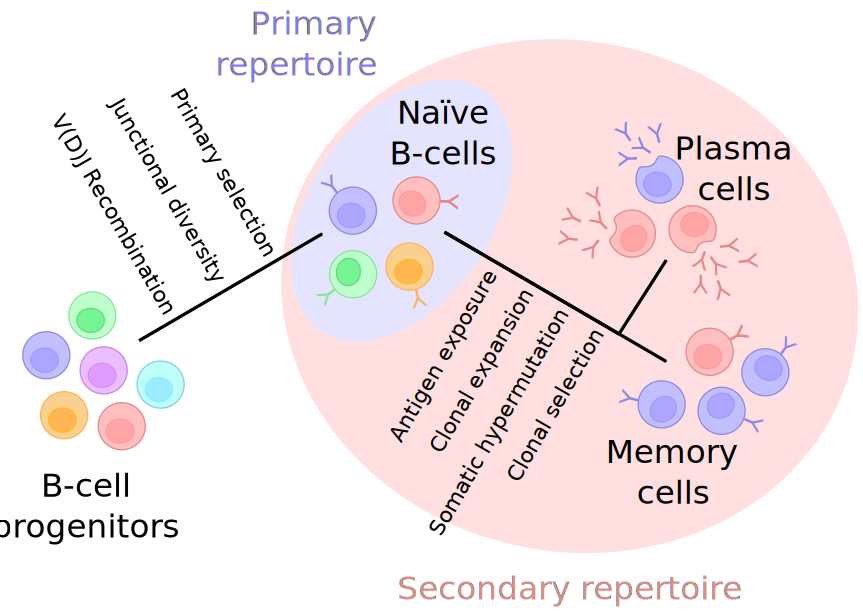
\includegraphics[width=0.9\textwidth]{output_files/figures/pdf/intro-bcell-repertoire-primary-secondary}
\Caption{Primary and secondary antibody repertoires}{Schematic of processes giving rise to the primary (\naive) and secondary (total) B-cell repertoires in the vertebrate immune system. Cell colours indicate clonal membership, with a loss of clonal diversity during primary development (left) and affinity maturation (right). Primary B-cell development (left) takes place in primary lymphoid organs (bone marrow in mammals, anterior kidney in teleosts \parencite{sunyer2013fishing}), while affinity maturation (right) takes place in germinal centres (in mammals) or proto-germinal clusters (in teleosts) in secondary lymphoid organs such as the gut-associated lymphoid tissue (GALT) or spleen \parencite{victora2012gc,magor2015affinity}.}
\label{fig:intro-bcell-repertoires}
\end{figure}

\section{Humoral adaptive immunosenescence in jawed vertebrates}
\label{sec:intro_immunosenescence}

The immune system of aged vertebrates has long been known to undergo a severe and systemic decline in functionality with age \parencite{segre1977immunosenescence}. As a result of this decline, older individuals exhibit increased susceptibility to a wide range of bacterial, viral, and fungal infectious diseases, as well as higher rates of complications and mortality from those infections when they occur \parencite{sambhara2009vaccination}. In addition, the effectiveness of vaccination against these infections often declines dramatically with age, with older individuals often receiving half or less of the immune protection from vaccination exhibited by younger recipients \parencite{sambhara2009vaccination}. Similar declines in immune functionality with age are also observed in other model organisms, and have been especially well-studied in mice, which share many details of their immune system with humans while being substantially easier to study in depth. While many different parts of the immune system are implicated in this immunosenescent phenotype \parencite{kogut2012bcells}, the decline in the humoral adaptive immune system has emerged as one particularly important contributor \parencite{ademokun2010ageing}.

The changes in the humoral immune system underlying its impaired functionality in old age begin at the level of B-cell development. In mice, the population of haematopoietic stem cells (HSCs) resident in the bone marrow increases in number but exhibits a decreased propensity to regenerate the pool of developing B-cells \parencite{ademokun2010ageing,kogut2012bcells}; factors contributing to this change include a deteriorating bone marrow niche, changes in blood-borne factors affecting HSC differentiation, and the well-known bias of older mammalian HSCs towards myeloid (rather than lymphoid) cell lineages \parencite{kogut2012bcells,dunnwalters2010bcellageing}. As a result of this change in HSC behaviour, the number of new B-cell progenitor and precursor cells in the bone marrow declines with age in mice; furthermore, these precursors exhibit decreased proliferation capacity, reduced rates of VDJ recombination and an increased rate of apoptosis \parencite{montecino2013immunosenescence,kogut2012bcells,labrie2004bone}. The rate of B-cell output from the bone marrow therefore declines significantly in aged mice, falling as low as 10\,\% of its level in young adults \parencite{kogut2012bcells}. As these \naive cells also have a shorter lifespan than antigen-experienced memory- and long-lived-plasma-cell populations, the net result of this decline in output from the bone marrow is a decrease in the number of \naive cells in the periphery and a progressive increase in the relative prevalence of antigen-experienced memory and plasma cells \parencite{mehr2011reversing,kogut2012bcells}; the pool of circulating immunoglobulins, meanwhile, becomes progressively dominated by hypermutated antibodies specific to previously-encountered antigens \parencite{kogut2012bcells}. As the \naive{}-cell pool is essential for responding to pathogenic threats not previously encountered by the immune system, this change is thought to lead to a progressive reduction in the capacity of the humoral immune system to respond effectively to these novel threats \parencite{kogut2012bcells}.

Despite the decline in new \naive B-cells produced by the bone marrow, the total number of B-cells in aged mice does not appear to change significantly, reflecting an increase in the absolute number, as well as the relative prevalence, of antigen-experienced B-cell subpopulations \parencite{ademokun2010ageing}. In humans, conversely, the absolute number of total B-cells appears to decline with age \parencite{ademokun2010ageing,montecino2013immunosenescence,aberle2013mechanistic}, with most B-cell subsets showing a significant decline in absolute abundance \parencite{frasca2011age}. Sources differ as to the age-related changes in relative abundance of different B-cell subtypes in humans, with some reporting an increase in the relative prevalence of \naive cells and decrease in that of memory cells \parencite{frasca2011age,blomberg2013age} and others reporting a more mouse-like shift in favour of the memory compartment \parencite{ademokun2010ageing}. These differences may arise from differences in the methods and cell markers used to quantify abundance of different B-cell populations \parencite{ademokun2010ageing}, genuine differences between populations, or the limitations of peripheral blood as a method of sampling the whole-body B-cell population of an individual \parencite{siegrist2009extremes,tabibiankeissar2016ageing}.

Whatever changes in cellular composition occur in ageing humans, it is clear that both humans and mice undergo a severe age-related decline in B-cell functionality. In humans, the best-understood aspect of this decline is a deterioration in the responsiveness of older patients to vaccination. Older humans frequently exhibit a substantially smaller \parencite{sambhara2009vaccination} and slower \parencite{kogut2012bcells} increase in the titre of antigen-specific serum antibodies in response to vaccination \parencite{sasaki2011limited,aberle2013mechanistic,ademokun2010ageing}, with defects in humoral response observed to vaccines for diseases as diverse as influenza, hepititis A and B, tetanus, diphtheria, pneumococcus and tick-borne encephalitis \parencite{dunnwalters2010bcellageing}. At least in the case of influenza, the observed decline in specific antibody production is primarily due to a decrease in the number of plasmablasts activated in response to vaccination \parencite{montecino2013immunosenescence,aberle2013mechanistic,sasaki2011limited}.

In addition to being less abundant, the antibodies produced by elderly humans in response to vaccination also appear to be of lower quality: anti-influenza antibodies produced by older human individuals demonstrate reduced ability to effectively neutralise viral haemagglutinin \parencite{kogut2012bcells,sasaki2011limited}, while \igh{M} antibodies produced by elderly subjects in response to pneumococcal polysaccharide vaccine demonstrate reduced opsonisation ability \parencite{kogut2012bcells}. While basal serum antibody titres actually increase with age in humans and mice \parencite{frasca2009ageing}, suggesting that antibody production \textit{per se} is not impaired, these antibodies also decline in quality \parencite{montecino2013immunosenescence}, with measurable increases in the rate of polyspecific and self-reactive antibodies produced in older individuals \parencite{kogut2012bcells}. This decline in baseline antibody quality in older individuals suggests a breakdown in primary B-cell selection in the bone marrow, enabling a greater number B-cells with low-specificity or self-reactive antibody sequences to emerge into the periphery \parencite{ademokun2010ageing}.

Various aspects of affinity maturation are also impaired in aged mammals. While memory-cell clones established early in life often persist into old age, \naive B-cells in aged humans demonstrate a severely reduced ability to give rise to new antigen-specific memory B-cells following antigenic stimulation, impairing the establishment of functional immune memory for novel threats \parencite{aberle2013mechanistic}. B-cells from older humans and mice also exhibit impaired class-switch recombination capacity, possibly as a result of decreased AID expression \parencite{montecino2013immunosenescence,blomberg2013age,frasca2011age}, impairing the generation of antibodies with the same specificity but different effector functions. The decreased ability of older individuals to produce high-affinity antigen-specific antibodies \parencite{frasca2011age} also suggests a defect in affinity maturation, though this could also be attributable to the known ageing-related defects in the T-helper and follicular dendritic cells involved in secondary B-cell selection \parencite{montecino2013immunosenescence,aberle2013mechanistic,ademokun2010ageing} rather than changes in the B-cells themselves. Conversely, the effect of ageing on the somatic hypermutation process remains controversial \parencite{henry2019influenza,howard2006quality,ademokun2010ageing,frasca2009ageing}, with different groups reporting an increase, a decrease, or no change in the rate and level of SHM accumulation of different B-cell subtypes with age. 

The various cellular and population-level changes that occur in the humoral immune system with age naturally have important effects on the antibody repertoires of ageing individuals. Aged humans \parencite{siegrist2009extremes} and mice \parencite{dunnwalters2010bcellageing} exhibit increased rates of non-malignant clonal expansions in the memory-cell compartment, which when combined with the apparent maintenance or decline in total B-cell number would lead to a reduction in overall diversity \parencite{dunnwalters2010bcellageing}. Similarly, early techniques that investigated the repertoire by investigating the distribution of CDR3 lengths (CDR3 spetratyping) indicated that older humans frequently exhibit more distorted distributions dominated by CDR3 regions of a particular length, indicative of clonal expansion, and found that older individuals with more distorted spectratypes exhibited greater frailty and worse health and lifespan outcomes than those with more young-like spectratypes \parencite{gibson2009spectratyping}. On the basis of these and similar findings, the antibody repertoire has long been thought to decline in diversity in older individuals, impairing the adaptability of the ageing adaptive immune system.

More recently, the development of specialised high-throughput-sequencing-based techniques for interrogating antibody repertoires (\Igseq, or \igseq \parencite{weinstein2009igseq,georgiou2014promise}) has enabled a few studies to investigate the ageing of these repertoires in greater detail. These studies, primarily on human peripheral blood, have confirmed many observations made using older lower-throughput methods: a reduced number of clonal lineages in older repertoires supports a decrease in \naive-cell output from the bone marrow \parencite{jiang2013vaccine}, while an increase in mean CDR3 length \parencite{wang2014ageing} and the rate of premature stop codons \parencite{debourcy2017ageing} support the finding that primary and clonal selection are impaired with age. An increase in clonal expansion with age is also observed in sequencing data: an oligoclonal phenotype, in which one or a few large clones dominate the repertoire, is often seen in peripheral blood from elderly humans but very rarely in the young \parencite{wang2014ageing,debourcy2017ageing}. These expanded clones are persistent before and after vaccination \parencite{debourcy2017ageing} and even across multiple years \parencite{wang2014ageing}; in contrast, large clones observed in young human blood repertoires are typically transient responses to recent antigen challenge \parencite{wang2014ageing}.

The reduction in clonal richness and increase in clonal expansions seen in older individuals contribute to an overall reduction in the estimated number of unique sequences present in the peripheral repertoire \parencite{debourcy2017ageing}, a change observed for both \naive and mutated sequences. The same study also found a drop in the percentage of unique sequences identified as coming from \naive B-cells, suggesting a mouse-like shift in repertoire prevalence towards antigen-experienced cell types \parencite{debourcy2017ageing}. However, while the alpha (within-individual) sequence diversity of the human peripheral repertoire appears to decline with age, the beta (between-individual) diversity of the repertoire actually increases, with repertoires from older individuals differing more from one another than those from young individuals do \parencite{debourcy2017ageing}. Elderly repertoires also showed decreased flexibility in response to immune challenge, with repertoires taken from the same individual pre- and post-vaccination being significantly more similar in elderly than in young samples \parencite{debourcy2017ageing}. Taken together, these findings suggest a pattern in which human peripheral antibody repertoires progressively lose diversity and flexibility over the course of the human lifespan, while also becoming increasingly individualised and distinct.

In conclusion, there is strong evidence for a variety of cellular and physiological changes in the B-cell immune system with age in both mice and humans, giving rise to a severe decline in functional performance and immune protection. Many of these changes affect the composition of the antibody repertoire, with a reduction in clonal and sequence diversity and an increase in between-individual variability with age in human blood. However, despite this abundance of data, there remain some serious limitations in our knowledge of the ageing antibody repertoire.  From an evolutionary and comparative perspective, almost nothing is known about adaptive immunosenescence in species other than humans and mice; while several \igseq studies have been performed on teleost fish \parencite{weinstein2009igseq,jiang2011determinism,krasnov2017igseq,lund2019salmon,fu2018fugu}, for example, none to my knowledge have investigated B-cell immunosenescence in this taxon. Many of the findings reported above are specific to \igh{G} or \igh{A} antibodies in mice and humans \parencite{kogut2012bcells}, and may not generalise to species lacking these isotypes. Even in humans, the majority of immunosenescence studies, including virtually all repertoire studies, are limited to peripheral blood, and therefore primarily sample the minority of B-cells in transition between tissues; the majority of B-cells, which are resident in some immune organ or tissue, are systematically underrepresented in these samples \parencite{siegrist2009extremes,tabibiankeissar2016ageing}. Relatively little is therefore known about how the ageing of the B-cell repertoire differs between organs; the only paper I know of which investigated changes in antibody-repertoire diversity with age in biopsies from multiple human tissues failed to find any significant changes in alpha diversity, except for a significant \textit{increase} in repertoire sequence entropy in old spleen \parencite{tabibiankeissar2016ageing}. To my knowledge, no publication has yet investigated the ageing of the antibody repertoire at mucosal surfaces, where secreted antibodies play a particularly important role in regulating microbiotal communities and defending the body from pathogenic invasion \parencite{belkaid2014microbiota}.

In addition to this lack of spatial resolution in our knowledge of antibody repertoire ageing, there is a serious lack of temporal resolution; most studies of antibody repertoire ageing simply compare a ``young'' group (say 20-30 years of age) with one or two ``old'' groups (say $\geq70$ years of age), with little or no information about the intervening progression of any observed phenotypes \parencite{debourcy2017ageing,tabibiankeissar2016ageing}. The effect of known lifespan-increasing interventions on immune-repertoire ageing also remains largely unstudied. Due to their very long lifespans and restrictions on experimental manipulation, humans are unsuitable subjects for these sorts of experiments, as are long-lived vertebrate model organisms such as zebrafish (median lifespan c. 3.5 years \parencite{gerhard2002zebrafish}) and \textit{Xenopus} (median lifespan c. 9 years \parencite{bowler1977longevity}). Even mice, though widely used in biogerontology, are inconveniently long-lived for many ageing experiments (median lifespan c. 2 to 2.5 years for the most common laboratory strains \parencite{yuan2009aging}). Conversely, many major model organisms in ageing research (such as fruit flies and nematode worms) are invertebrates, and so lack a mammal-like adaptive immune system. The development of a short-lived vertebrate species as a model organism for antibody-repertoire experiments would therefore be highly valuable for research into adaptive immunosenescence.

\section{The African turquoise killifish as a model for vertebrate ageing}
\label{sec:intro_killifish}

The genus \textit{Nothobranchius} comprises a broad group of annual freshwater fishes distributed across equatorial and subequatorial Africa \parencite{valdesalici2003lifespan}, with species diversity concentrated in the south-east of the continent \parencite{genade2005annual}. Members of this genus share a suite of adaptations to life in ephemeral pools and rivers, most notably the production of desiccation-resistant embryos capable of surviving through the dry season in a diapause state \parencite{genade2005annual} (\Cref{fig:intro-killifish-life-cycle}). Fish from this genus have been known for several decades to  exhibit very rapid growth and short lifespans, consistent with their evolving under conditions of very high extrinsic mortality \parencite{valdesalici2003lifespan}, with many species exhibiting a median lifespan of less than one year. Nevertheless, there is wide variation within the genus in body size, growth rate and lifespan, with species from less arid regions tending to show slower growth and longer median lifespans \parencite{genade2005annual}.

Like other \textit{Nothobranchius} species, the turquoise killifish (\nfu, \Cref{fig:intro-killifish-photos}) is a medium-sized annual fish first isolated from ephemeral freshwater pools -- in this case, from a relatively arid region of southeastern Zimbabwe and Mozambique \parencite{genade2005annual,jubb1971new}. Even by the standards of the \textit{Nothobranchius} genus, \Nfu exhibits extremely rapid growth, maturation, and ageing, with the most widely-used laboratory strain (GRZ) exhibiting a median lifespan of just 9-16 weeks \parencite{valdesalici2003lifespan,genade2005annual,terzibasi2008strains,kirschner2012map,valenzano2015genome,smith2017microbiota} (\Cref{fig:intro-killifish-lifespan}) -- the shortest lifespan of any captive-bred vertebrate, and a dramatic outlier on the distribution of vertebrate lifespans (\Cref{fig:intro-killifish-comparison}). Combined with their possession of several important vertebrate-specific adaptations -- including an adaptive immune system -- this extremely short lifespan makes the turquoise killifish a highly promising model organism for ageing research \parencite{harel2016crispr}.

Despite its very short lifespan, \textit{N. furzeri} has been found to show a wide range of senescent phenotypes in even the shortest-lived strains, including lipofuscin deposition \parencite{genade2005annual};  accumulation of senescence markers \parencite{genade2005annual};  increased neurodegeneration \parencite{valenzano2006resveratrol1,valenzano2006resveratrol2}; impaired learning and behavioural phenotypes  \parencite{genade2005annual,valenzano2006resveratrol1}; and a high incidence of degenerative and neoplastic lesions \parencite{dicicco2011histopathology}. These diverse phenotypes indicate that the short lifespan of the turquoise killifish is the result of an accelerated general ageing process, rather than the specific failure of a particular organ or system. Moreover, established anti-ageing interventions such as resveratrol treatment \parencite{valenzano2006resveratrol1}, reduction in ambient temperature \parencite{valenzano2006temperature} and dietary restriction \parencite{terzibasi2009dr} also extend lifespan in the turquoise killifish, indicating a strong analogy with the ageing phenotypes observed in canonical model systems.

Due primarily to its potential as a model organism for ageing research, the turquoise killifish has also seen rapid development as a genetic model. The short-lived GRZ strain has been bred in captivity for fifty years and at least a hundred generations \parencite{terzibasi2007review} and exibits a very high degree of homozygosity \parencite{kirschner2012map,reichwald2009genome,valenzano2009map}, providing a uniform genetic background for experimental interventions. A number of important genetic resources are now available, including several assemblies of the nuclear genome \parencite{reichwald2015genome,valenzano2015genome,willemsen2019popgen}, the most recent of which \parencite{willemsen2019popgen} is of very high quality. These assemblies have yielded a genome with an estimated size of roughly 1.5 gigabases \parencite{willemsen2019popgen};
karyotyping \parencite{reichwald2009genome} and sequencing analysis \parencite{reichwald2015genome} both indicate a chromosome number of $2n = 38$, corresponding to 19 distinct linkage groups in the haploid genome.

Prior to the work contained in this thesis, almost nothing was known about the adaptive immune system of the turquoise killifish. However, as a teleost, and therefore as a jawed vertebrate, it could be strongly expected to have a roughly mammal-like adaptive immune system, and a number of genes related to B-cell adaptive immunity (including \gene{RAG1}, various B-cell developmental markers, and fragments of antibody genes) were identified in one or more genome annotations. Phylogenetically, the genus \textit{Nothobranchius} falls within the Cyprinodontiformes, and the turquoise killifish is therefore relatively closely related to several species with previously-characterised \igh{} loci, including fugu, stickleback and medaka \parencite{terzibasi2007review,hughes2018teleostphylo}. Despite the relatively unknown state of adaptive immunity in the turquoise killifish, therefore, there was good reason to believe it possessed a functional B-cell immune system similar to those of other teleosts, and therefore comparable in many respects with those of mammalian species, including humans. When combined with its short lifespan and rapid ageing phenotype, this made the turquoise killifish a potentially highly-valuable model for studying the forms and mechanisms of humoral adaptive immunosenescence in jawed vertebrates. % TODO: Break paragraph here? (If relating findings)

In this thesis, therefore, I characterised the \igh{} locus of the turquoise killifish (\Cref{chap:locus}), established a working \Igseq protocol for killifish samples, and performed the first experiments investigating adaptive immunosenescence in this species (\Cref{chap:igseq}). The results demonstrated that turquoise killifish possess a complex and sophisticated adaptive immune system with diverse and individualised antibody repertoires, which nevertheless undergoes a rapid loss of within-individual diversity with age. This loss of diversity was especially pronounced in isolated gut samples, possibly due to the intense antigenic exposure experienced at mucosal surfaces. Taken together, these results confirm the value of the turquoise killifish as a model system for investigating adaptive immunosenescence in vertebrates.

% TODO: Dario: state your findings again here

\begin{figure}
\centering
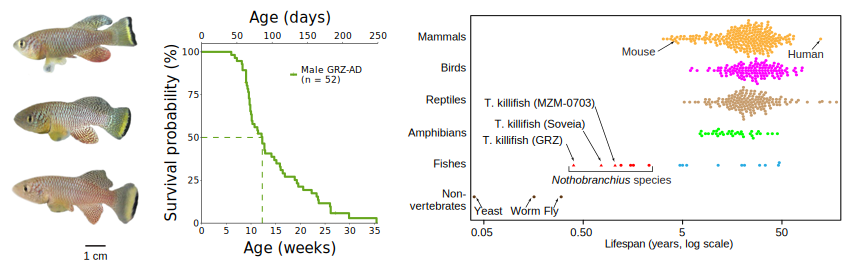
\includegraphics[width=0.95\textwidth]{output_files/figures/pdf/intro-turquoise-killifish}
\begin{subfigure}{0em}
\phantomsubcaption{}
\label{fig:intro-killifish-photos}
\end{subfigure}
\begin{subfigure}{0em}
\phantomsubcaption{}
\label{fig:intro-killifish-life-cycle}
\end{subfigure}
\begin{subfigure}{0em}
\phantomsubcaption{}
\label{fig:intro-killifish-lifespan}
\end{subfigure}
\begin{subfigure}{0em}
\phantomsubcaption{}
\label{fig:intro-killifish-comparison}
\end{subfigure}
\Caption{The turquoise killifish (\nfu) as a model for vertebrate ageing}{(A) Photographs of adult male yellow-tailed turquoise killifish.
(B) Life cycle of the turquoise killifish in its natural environment, showing hatching and breeding during the rainy season and embryo survival in diapause during the dry season.
(C) Example lifespan curve of short-lived GRZ-AD turquoise-killifish males, hatched in December 2016, with a median lifespan of roughly 12 weeks.
(D) Comparison of turquoise-killifish maximum lifespan (red triangles) to other vertebrate species, demonstrating the extremely short lifespan of GRZ-strain \Nfu compared to other vertebrates. (A), (B) and (D) adapted from \parencite{valenzano2015genome}, Figure 1.}
\label{fig:intro-killifish}
\end{figure}

\chapter{Materials and methods}  
\onehalfspacing

\ifdefineChapter
	{\LARGE Second Draft, \today}
\fi

\pagebreak

\section{Killifish husbandry and sample-preparation methods}
\label{sec:methods_husbandry}

Male turquoise killifish (\nfu, GRZ-AD strain) from a single hatching were raised under standard husbandry conditions \parencite{dodzian2018husbandry} and housed from four weeks post-hatching in individual \lt{2.8} tanks connected to a water-recirculation system. Fish received \hr{12} of light per day on a regular light/dark cycle, and were fed blood
worm larvae and brine shrimp nauplii twice a day during the week and once a day during the weekend \parencite{dodzian2018husbandry,smith2017microbiota}.

Sacrificed fish (\Cref{tab:igseq-cohorts-fish}) were killed by anaesthetisation in \gl{1.5} Tricaine solution in room-temperature tank water \parencite{carter2011tricaine}, then flash-frozen in liquid nitrogen and ground to a homogenous powder with a pestle in a liquid-nitrogen-filled mortar. The powder was mixed thoroughly and stored at \degC{-80} prior to RNA isolation.

\section{Biochemistry and molecular-biology methods}

\subsection{Standard laboratory techniques}

\subsubsection{PCR}
\label{sec:methods_molec_standard_pcr}

The polymerase chain reaction is a well-established method for rapid amplification of a DNA sequence through repeated cycles of denaturation, primer-annealing and replication by a high-temperature-tolerant DNA polymerase enzyme \parencite{paul2010hotstartpcr}. Unless otherwise specified, all PCRs in this chapter were performed using \x{2} Kapa HiFi HotStart ReadyMix PCR Kit (\Cref{app:solutions_enzymes}) according to the manufacturer's instructions. Briefly, for a \ul{25} reaction, \ul{12.5} Kapa ReadyMix was combined with \ul{12.5} total of template, nuclease-free water, and \umol{10} primers; these volumes were scaled linearly for reactions of different volumes. The mixture was then heated in a thermocycler as described in \Cref{tab:kapa}.

\begin{table}[h]
\centering
\caption{Thermocycler protocol for Kapa high-fidelity hot-start PCR}
\label{tab:kapa}
\begin{threeparttable}
\begin{tabular}{cccc}\toprule
\textbf{Step} & \textbf{Temperature (\degC{})} & \textbf{Duration (\secs{})} & \textbf{\# Cycles}\\\midrule
Initial denaturation & 95 & 180 & 1 \\\midrule
Denaturation & 98 & 20 & \multirow{3}{*}{$n_c$\tnote{a}}\\
Annealing & $T_a$\tnote{a} \tnote{} & 15 & \\
Extension & 72 & $t_{ext}$\tnote{a} & \\\midrule
Final extension & 72 & $t_{ext} \times 4$\tnote{a} & 1\\
\bottomrule\end{tabular}
\begin{tablenotes}
\item[a] Annealing temperature ($T_a$), extension time ($t_{ext}$) and cycle number ($n_c$) determined separately for each reaction.
\end{tablenotes}
\end{threeparttable}
\end{table}

\subsubsection{Nucleic-acid purification with SeraSure magnetic beads}
\label{sec:methods_molec_standard_serasure}

Nucleic-acid isolation, size-selection and concentration in the \igseq library-preparation protocol (and elsewhere where necessary) were performed using SeraSure SPRI (solid-phase reversible immobilisation) bead preparations \parencite{hawkins1994spri,deangelis1995spri,lennon2010cleanup,fisher2011cleanup}. In SPRI, carboxyl-coated paramagnetic beads bind DNA in the presence of polyethylene glycol (PEG), with the affinity of the beads for DNA depending on the concentration of PEG in the binding buffer. As a result, the range of nucleic-acid sequence lengths retained by SPRI bead purification depends primarily on the concentration of PEG, which in turn depends on the relative volume of SeraSure bead suspension added to a sample; the higher the concentration, the shorter the minimum fragment length retained during the purification process. In combination with a magnetic rack to remove the DNA-bound beads from suspension, this allows DNA of the desired size range to be isolated from a solution and resuspended in the desired volume of fresh buffer.

To prepare \ml{50} of SeraSure bead suspension for DNA (or DNA:RNA heteroduplex) isolation, a stock of SeraMag beads (\Cref{app:solutions_reagents}) was vortexed thoroughly, and \ml{1} was transferred to a new tube. This tube was then transferred to a magnetic rack and incubated at room temperature for \mins{1}, then the supernatant was removed and replaced with \ml{1} TET buffer (\Cref{app:solutions_buffers}) and the tube was removed from the rack and vortexed thoroughly. This washing process was repeated twice more, for a total of three washes in TET. A fourth cycle was used to replace the TET with incomplete SeraBind buffer (iSB, \Cref{app:solutions_buffers}). The vortexed \ml{1} aliquot of beads in iSB was then transferred to a conical tube containing \ml{28} iSB and mixed by inversion. To add the PEG, \ml{20} \pc{50} (w/v) PEG 8000 solution was dispensed slowly down the side of the conical tube, bringing the total volume to \ml{49}. Finally, this was brought to \ml{50} by adding \ul{250} \pc{10} (w/v) Tween 20 solution and \ul{750} autoclaved water to complete the SeraSure bead suspension.

To perform a bead cleanup, an aliquot of prepared SeraSure suspension was vortexed thoroughly to completely resuspend the beads, then the appropriate relative volume of SeraSure suspension was added to a sample, mixing thoroughly by gentle pipetting. The sample was incubated at room temperature for \mins{5} to allow the beads to bind the DNA, then transferred to a magnetic rack and incubated for a further \mins{5} to draw as many beads as possible out of suspension. The supernatant was removed and discarded and replaced with \pc{80} ethanol, to a volume sufficient to completely submerge the bead pellet. The sample was incubated for 0.5-\mins{1}, then the ethanol was replaced and incubated for a further 0.5-\mins{1}. The second ethanol wash was removed, and the tube left on the rack until the bead pellet was almost, but not completely, dry, after which it was removed from the rack. The bead pellet was resuspended in a suitable volume of elution buffer (EB, \Cref{app:solutions_buffers}) then incubated at room temperature for at least 5 minutes to allow the nucleic-acid molecules to elute from the beads.

Unless otherwise specified, the beads from a cleanup were left in a sample during subsequent applications. To remove beads from a sample, the sample was mixed gently but thoroughly to resuspend the beads, incubated for an extended time period (at least \mins{10}) to maximise nucleic-acid elution, then transferred to a magnetic rack and incubated for 2-\mins{5} to remove the beads from suspension. The supernatant (containing the eluted nucleic-acid molecules) was then transferred to a new tube, and the beads discarded.

\subsubsection{Phenol-chloroform extraction and ethanol precipitation of DNA}
\label{sec:methods_molec_standard_phenol}

Phenol-chloroform extraction is a well-established method for removing proteins and other hydrophobic or amphipathic contaminants from nucleic-acid solutions \parencite{zumbo2012phenolchloroform}. By thoroughly mixing an aqueous solution of nucleic acid with an organic solvent (phenol), hydrophobic contaminants are dissolved into the organic phase while proteins are denatured at the organic/aqueous boundary. The addition of chloroform further encourages the denaturation of proteins, as well as improving separation of the aqueous and organic phases following centrifugation. The effect on nucleic acids depends upon the pH of the phenol: under acidic conditions, the negatively-charged DNA phosphate backbone is neutralised and so primarily dissolves in the organic phase, while RNA is kept in the aqueous phase through hydrogen bonding between water and exposed bases; under neutral or basic conditions, both DNA and RNA are retained in the aqueous phase \parencite{zumbo2012phenolchloroform}.

To remove protein from isolated DNA samples, each sample was diluted to \ul{500} in nuclease-free water and mixed with \ul{500} of equilibrated (non-acidic) phenol:chloroform:isoamyl alcohol (PCI) mixture (\Cref{app:solutions_reagents}) in a fume hood. The sample/PCI mixture was shaken vigorously by hand for \secs{15} to thoroughly mix the different components, then centrifuged in a benchtop centrifuge (\mins{5}, room temperature, top speed). Again in a fume hood, the mixed sample was held at an angle, and the upper aqueous phase containing the DNA was removed and transferred to a new tube while the lower organic phase was discarded. A second aliquot of \ul{500} PCI was added and the sample was mixed, centrifuged and separated as before. Finally, in order to remove residual phenol in the sample, \ul{500} pure chloroform was added to the newly-separated aqueous phase and the sample was once again mixed, centrifuged and separated. 

Following this final round of separation, the DNA in the aqueous phase was re-isolated using ethanol precipitation, another widely-used protocol exploiting the ability of alcohols to precipitate nucleic acids in the presence of monovalant cations \parencite{zumbo2012ethanol}. 0.1 volumes of \mol{3} sodium acetate solution was added to each sample, followed by 2.5 volumes of fresh \pc{100} ethanol. The mixture was mixed gently by inversion, then incubated for 1-\hr{3} at \degC{-80} or at \degC{-20} overnight. The suspension of precipitated DNA was pelleted through centrifugation in a benchtop centrifuge (\mins{30}, \degC{4}, top speed). The supernatant was discarded and replaced with \ul{500} chilled \pc{70} ethanol, and the sample centrifuged again (\mins{5}, \degC{4}, top speed). After this, the supernatant was again discarded, and the samples allowed to air-dry before being resuspended in 30-\ul{50} EB (\Cref{app:solutions_buffers}). 

\subsubsection{Guanidinium thiocyanate-phenol-chloroform extraction of RNA}
\label{sec:methods_molec_standard_qiazol}

Guanidinium thiocyanate-phenol-chloroform extraction is a technique for purifying RNA samples closely related to the phenol-chloroform-extraction method described in \Cref{sec:methods_molec_standard_phenol} \parencite{zumbo2012phenolchloroform}. By using acid rather than equilibrated phenol, DNA in the sample is dissolved in the organic rather than the aqueous phase and so is removed from the aqueous solution along with proteins and other contaminants \parencite{zumbo2012phenolchloroform,chomczynski2006trizol}. Meanwhile, the addition of guanidinium thiocyanate, a chaotropic agent which disrupts hydrogen bonds in aqueous solution, strongly encourages the rapid denaturation of proteins and so helps protect the RNA from degradation by RNase enzymes \parencite{zumbo2012phenolchloroform,chomczynski2006trizol}.

To isolate total RNA from homogenised killifish tissues, \ml{1} of QIAzol lysis reagent (\Cref{app:solutions_reagents}, containing acid phenol and guanidinium thiocyanate) was added to \gr{0.1} of tissue, mixed gently but thoroughly by inversion, then incubated at room temperature for \mins{5} to allow the QIAzol to penetrate the tissue. 0.2 volumes of chloroform was added and the mixture was shaken vigorously for \secs{15}, then incubated at room temperature for \mins{3}. The mixture was then centrifuged (\mins{15}, \degC{4}, \g{12000}). Holding the tube at an angle, the upper aqueous phase containing the RNA was removed and transferred to a new tube, while the lower organic phase was discarded.

Following phase separation, the RNA was precipitated using isopropanol precipitation, which works on the same principles as ethanol precipitation (\Cref{sec:methods_molec_standard_phenol}) but requires shorter incubation times and lower relative volumes of alcohol \parencite{zumbo2012ethanol}. 0.5 volumes of room-temperature isopropanol was added to each sample, mixing gently by inversion and incubating for \mins{5} at room temperature. The suspension was centrifuged (\mins{10}, \degC{4}, \g{12000}) and the supernatant discarded. 1 volume of freshly prepared \pc{75} ethanol was added and the tube was vortexed briefly and centrifuged again (\mins{5}, \degC{4}, \g{7500}). The supernatant was discarded and the RNA pellet allowed to air-dry for 5-\mins{10}, then resuspended in \ul{50} EB (\Cref{app:solutions_buffers}). The concentration and quality of the resulting total-RNA solution were assayed with the Qubit 2.0 flourometer (Thermo Fisher, RNA BR assay kit) and TapeStation 4200 (Agilent, RNA tape), respectively, according to the manufacturer's instructions.

\subsection{Library size-selection with the BluePippin}
\label{sec:methods_molec_standard_bluepippin}

The BluePippin (Sage Science) is a DNA size-selection system based on agarose gel electrophoresis, which uses timed switching between positively-charged electrodes at a forked gel channel in an agarose cassette to redirect DNA of a desired size range into a separate lane from the rest of the sample \parencite{sage2016bluepippin}. The timing of the switch is determined based on the size range input by the user and calibrated using flourescent internal standards, which are added to the sample during the preparation process and designed to run well ahead of the possible size ranges for that cassette type. The combination of the choice of cassette and the choice of standards determines which fragment lengths can be effectively isolated using the machine.

For the experiments described in this thesis, a \pc{1.5} cassette with R2 markers was used, enabling size selection of targets in the range of 250--\bp{1500} \parencite{sage2016bluepippin}. Machine calibration and testing, cassette preparation, and protocol design were performed in accordance with the BluePippin documentation and instructions given by the machine software. During this process, the elution wells of the lanes to be used in the size-selection run were emptied and refilled with \ul{40} of electrophoresis buffer (\Cref{app:solutions_reagents}), then sealed for the duration of the run, and a broad-range size-selection protocol with a target range of 400 to \bp{800} was specified. \ul{30} of sample was then combined with \ul{10} of loading solution (\Cref{app:solutions_reagents}) and vortexed to mix, then \ul{40} of buffer was removed from the appropriate loading well and replaced, slowly, with the prepared sample mixture. The protocol was started and run until the final elution was complete. Finally, the eluted samples were removed from the elution wells of the appropriate lanes, and the unused lanes of the cassette were re-sealed for future use.

\subsection{Isolation and sequencing of bacterial artificial chromosomes}
\label{sec:methods_molec_bacs}

All BAC clones that were sequenced for this research were provided by the FLI in Jena as plate or stab cultures of transformed \textit{E. coli}, which were replated and stored at \degC{4}. Prior to isolation, the clones of interest were cultured overnight in at least \ml{100} LB medium. The resulting liquid cultures were transferred to \ml{50} conical tubes and centrifuged (10-\mins{25}, \degC{4}, \g{3500}) to pellet the cells. The supernatant was carefully discarded and the cells were resuspended in \ml{18} buffer P1 (\Cref{app:solutions_buffers}).

After resuspension, the cultures underwent alkaline lysis \parencite{birnboim1979alkalinelysis} to release the BAC DNA and precipitate genomic DNA and cellular debris. \ml{18} buffer P2 (\Cref{app:solutions_buffers}) was added to each tube, which was then mixed gently but thoroughly by inversion and incubated at room temperature for \mins{5}. \ml{10} ice-chilled neutralisation buffer P3 (\Cref{app:solutions_buffers}) was added to precipitate genomic DNA and cellular debris, and each tube was mixed gently but thoroughly by inversion and incubated on ice for \mins{15}. The tubes were then centrifuged (20-\mins{30}, \degC{4}, \g{12000}) to pellet cellular debris and the supernatant was transferred to new conical tubes. This process was repeated at least two more times, until no more debris was visible in any tube; this repeated pelleting was necessary to minimise contamination in each sample, as the normal column- or paper-based filtering steps used during alkaline lysis resulted in the loss of the BAC DNA.

Following alkaline lysis, the DNA in each sample underwent isopropanol precipitation: 0.6 volumes of room-temperature isopropanol were added to the clean supernatant in each tube, followed by 0.1 volumes of \mol{3} sodium acetate solution. Each tube was mixed well by inversion, incubated for 10-\mins{15} at room temperature, then centrifuged (\mins{30}, \degC{4}, \g{12000}) to pellet the DNA. The supernatant was discarded and the resulting DNA smear was ``resuspended'' in \ml{1} \pc{100} ethanol and transferred to a \ml{1.5} tube, which was re-centrifuged (\mins{5}, \degC{4}, top speed) to obtain a concentrated pellet. Finally, the pelleted samples were resuspended in EB (\Cref{app:solutions_buffers}) and purified of proteins and RNA using phenol-chloroform extraction and ethanol precipitation (\Cref{sec:methods_molec_standard_phenol}).

The resuspended BAC isolates were sent to the Cologne Center for Genomics, where they underwent Illumina Nextera XT library preparation and were sequenced on an Illumina MiSeq sequencing machine (MiSeq Reagent Kit v3, 2$\times$\bp{300} reads).

\subsection{Immunoglobulin sequencing of killifish samples}
\label{sec:methods_molec_igseq}

\subsubsection{RNA template quantification and quality control}
\label{sec:methods_molec_igseq_template}

Total RNA from whole-body killifish samples was isolated as described in \Cref{sec:methods_molec_standard_qiazol}; gut RNA from microbiota-transfer experiments \parencite{smith2017microbiota} was already prepared and available. Quantification of RNA samples was performed with the Qubit 2.0 flourometer (Thermo Fisher, RNA BR assay kit), while quality control and integrity measurement was performed using the TapeStation 4200 (Agilent, RNA tape), both according to the manufacturer's instructions.

\subsubsection{Reverse transcription and template switching}
\label{sec:methods_molec_igseq_rt}

Reverse transcription of total RNA and template switching for \igseq library preparation was performed using SMARTScribe Reverse Transcriptase (\Cref{app:solutions_enzymes}), in line with the protocol specified in Turchaninova \textit{et al.} \parencite{turchaninova2016igprep}. Briefly, \ng{750} total RNA from a killifish sample was combined with \ul{2} \umol{10} gene-specific primer (GSP), homologous with the second \ch exon of \Nfu \igh{M} (\Cref{app:oligos_primers}, designed using \program{Primer3} \parencite{untergasser2012primer3}). The reaction volume was brought to a total of \ul{8} with nuclease-free water, and the resulting mixture was incubated for 2 minutes at \degC{70} to denature the RNA, then cooled to \degC{42} to anneal the GSP \parencite{turchaninova2016igprep}.

Following annealing, the RNA-primer mixture was combined with \ul{12} of reverse-transcription master-mix (\Cref{tab:methods_rt_mm}), including the reverse-transcriptase enzyme and template-switch adapter (\Cref{app:oligos_tsa}, sequence provided in \parencite{turchaninova2016igprep}). The complete reaction mixture was incubated for \hr{1} at \degC{42} for the reverse-transcription reaction, then mixed with \ul{1} of uracil DNA glycosylase (UDG, \Cref{app:solutions_enzymes}) and incubated for a further \mins{40} at \degC{37} to digest the template-switch adapter. Finally, the reaction product was purified using SeraSure beads (\Cref{sec:methods_molec_standard_serasure}, \Cref{tab:methods_igseq_beads}).

\begin{table}[h]
\begin{center}\small
\begin{threeparttable}
\caption[Master-mix components for SMARTScribe reverse transcription]{Master-mix components for SMARTScribe reverse transcription (per sample)}
\begin{tabular}{llll}\toprule
\textbf{Volume (\ul{})} & \textbf{Component} & \textbf{Initial concentration} & \textbf{Reference}\\\midrule
2 & SMARTScribe reverse transcriptase & \unitsul{100} & \Cref{app:solutions_enzymes} \\
4 & SMARTScribe first-strand buffer & \x{5} & \Cref{app:solutions_reagents} \\
2 & SmartNNNa barcoded TSA & \umol{10} & \Cref{app:oligos_tsa}\\
2 & DTT & \mmol{20} & \Cref{app:solutions_reagents}\\
2 & dNTP mix & \umol{10} per nucleotide & \Cref{app:solutions_reagents}\\
0.5 & RNasin RNase inhibitor & \unitsul{40} & \Cref{app:solutions_enzymes}\\\bottomrule
\end{tabular}
\label{tab:methods_rt_mm}
\end{threeparttable}
\end{center}
\end{table}

\subsubsection{PCR amplification and adapter addition} 
\label{sec:methods_molec_igseq_pcr}

Following reverse transcription, UDG digestion, and cleanup, the reaction mixture underwent three successive rounds of Kapa PCR (\Cref{sec:methods_molec_standard_pcr}, \Cref{tab:methods_igseq_pcr}) each of which was followed by a further round of bead cleanups (\Cref{sec:methods_molec_standard_serasure}, \Cref{tab:methods_igseq_beads}). The first of these PCR reactions added a second strand to the reverse-transcribed cDNA and amplified the resulting DNA molecules; the second added partial Illumina sequencing adapters and further amplified the library, and the third added complete Illumina adapters (\Cref{app:oligos_illumina}, including i5 and i7 indices \parencite{illumina2018adapters}). Primer sequences (\Cref{app:oligos_primers}) homologous to the template-switch adapter (M1SS and M1S) were provided by Turchaninova \textit{et al.} \parencite{turchaninova2016igprep}, while those homologous to the \cm{1} constant-region exon (IGHC-B and IGHC-C) were designed using \program{Primer3} \parencite{untergasser2012primer3}.

\begin{table}[h]
\def\arraystretch{1.3}
\centering\small
\begin{threeparttable}
\caption{PCR protocols for \Nfu immunoglobulin sequencing}
\begin{tabular}{c|ccc|cc|ccccc}\toprule
\multirow{2}{*}{\textbf{PCR}} & \multicolumn{3}{c|}{\textbf{Protocol details}} & \multicolumn{2}{c|}{\textbf{Primers}} & \multicolumn{4}{c}{\textbf{Volumes (\ul{})\tnote{b}}}\\
 & \# cycles & $T_m$ (\degC{}) & $t_\mathrm{ext}$ (\secs{}) & F & R & Template & Primers\tnote{c} & Kapa & H\textsubscript{2}O \\\midrule
1 & 18 & 65 & 15 & IGHC-B & M1SS & 10.5 & 1 (\x{}2) & 12.5 & 0 \\\midrule
2 & 13 & 65 & 15 & M1S+P2 & IGHC-C+P1 & 1 & 0.5 (\x{}2) & 12.5 & 10.5 \\\midrule
3 & 8 to 12\tnote{d} & 68 & 15 & D50*\tnote{a} & D7**\tnote{a} & 2 & 0.75 (\x{}2) & 12.5 & 9 \\
\bottomrule
\end{tabular}
\begin{tablenotes}
\item[a] PCR3 primers selected as appropriate for each library's assigned indices; see \Cref{app:oligos_illumina} for more information.
\item[b] If the number of samples to be sequenced was small, all volumes of PCR 3 were doubled for a \ul{50} total PCR volume.
\item[c] The stated volumes apply separately to both forward and reverse primers for each reaction. All primers were diluted to and stored at an initial concentration of \umol{10}.
\item[d] See \Cref{tab:methods_igseq_cycles} for specific cycle numbers used in each experiment.
\end{tablenotes}
\label{tab:methods_igseq_pcr}
\end{threeparttable}
\end{table}

\begin{table}[h]
\def\arraystretch{1.5}
\centering\small
\caption{Bead cleanups during \Nfu immunoglobulin sequencing}
\begin{threeparttable}
\begin{tabular}{l|c|cc|c}\toprule
\multirow{2}{*}{\textbf{Stage}\tnote{a}} & \multirow{2}{*}{\textbf{Sample volume}} & \multicolumn{2}{c|}{\textbf{Beads volume (\ul{})}} & \multirow{2}{*}{\textbf{Elution volume (\ul{})}\tnote{c}}\\
& & \ul{} & \x{}\tnote{b} & \\\midrule
RT & 21 & 14.7 & 0.7 & 16.5\\
PCR 1 & 25 & 17.5 & 0.7 & 25\\
PCR 2 & 25 & 17.5 & 0.7 & 15\\
PCR 3 & 25\tnote{d} & 20\tnote{d} & 0.8 & 15\tnote{d}\\
Pooling & Varies\tnote{e} & Varies\tnote{e} & 2.5 & 35\\ 
\bottomrule
\end{tabular}
\begin{tablenotes}
\item[a] Each bead cleanup takes place immediately \textit{after} its corresponding stage.
\item[b] Bead volumes are usually given as multiples of the sample volume.
\item[c] All elutions performed in the specified volume of elution buffer (EB, \Cref{app:solutions_buffers}).
\item[d] If the PCR 3 reaction volume differed from \ul{25}, bead and elution volumes were rescaled proportionally to sample volume as appropriate.
\item[e] Samples are pooled in equimolar ratio.
\end{tablenotes}
\label{tab:methods_igseq_beads}
\end{threeparttable}
\end{table}

\begin{table}[h]
\def\arraystretch{1.3}
\centering\small
\caption{PCR cycle numbers during \Nfu immunoglobulin sequencing}
\begin{threeparttable}
\begin{tabular}{c|ccc|cc|ccccc}\toprule
\multirow{2}{*}{\textbf{Experiment}} & \multicolumn{3}{c|}{\textbf{Number of PCR cycles}} & \multirow{2}{*}{\textbf{Reference}}\\
& PCR 1 & PCR 2 & PCR 3 &\\\midrule
Pilot & 18 & 13 & 9 & \Cref{sec:igseq_pilot}\\
Ageing & 18 & 13 & 8 & \Cref{sec:igseq_ageing}\\
Gut & 18 & 13 & 12 &\Cref{sec:igseq_gut}\\
\bottomrule
\end{tabular}
\label{tab:methods_igseq_cycles}
\end{threeparttable}
\end{table}

\subsubsection{Library pooling, size selection and sequencing} 
\label{sec:methods_molec_igseq_seq}

Following PCR3 and its attendant bead cleanup, the total concentration of each library was assayed with the Qubit 2.0 (Thermo Fisher, DNA HS assay kit), while the size distribution of each library was obtained using the TapeStation 4200 (Agilent, D1000 tape). To obtain the concentration of complete library molecules in each case (as opposed to primer dimers or other off-target bands), the ratio between the concentration of the desired library band (c. 620-\bp{680}) and the total concentration of the sample was calculated for each TapeStation lane, and the total concentration of each library as measured by the Qubit was multiplied by this ratio to obtain an estimate of the desired quantity:

\begin{equation}
\mathrm{Library~concentration}~(L) = \mathrm{Qubit~concentration} \times \frac{\mathrm{TapeStation~concentration~[main~band]}}{\mathrm{TapeStation~concentration~[total]}}
\label{eq:library-conc}
\end{equation}

\noindent All the libraries for a given experiment were then pooled, such that the estimated concentration $L$ of each library in the final pooled sample was equal and the total mass of nucleic acid in the pooled sample was at least \ng{240}. The pooled libraries underwent a final bead cleanup (\Cref{sec:methods_molec_standard_serasure}, \Cref{tab:methods_igseq_beads}) to concentrate the samples, then underwent size selection with the BluePippin (\Cref{sec:methods_molec_standard_bluepippin}, \pc{1.5} DF Marker R2, broad 400-800bp). The size-selected pooled samples underwent a final round of quality control with the Qubit and TapeStation (as above) to confirm their collective concentration (at least \nmol{1.5}) and size distribution (one peak at c. 620-\bp{680}). Finally, the pooled and size-selected libraries were sequenced on an Illumina MiSeq System (MiSeq Reagent Kit v3, 2$\times$\bp{300} reads, 30\,\% PhiX spike-in), either at the Cologne Center for Genomics (pilot and ageing experiments) or with Admera Health (gut experiment).

\section{Computational and analytic methods}
\label{sec:methods_comp}

Version details for software used in this section are given in \Cref{tab:software-versions}.

\subsection{General data processing, pipeline structure, and data visualisation}
\label{sec:methods_comp_general}

Unless otherwise specified, processing and analysis of biological data was performed using standard Bioconductor \parencite{huber2015bioconductor} packages: \program{Biostrings} \parencite{pages2017biostrings} and \program{BSgenome} \parencite{pages2018bsgenome} for biological sequence data, \program{GenomicRanges} \parencite{lawrence2013genomicranges} for sequence ranges, and \program{genbankr} \parencite{becker2018genbankr} and \program{rentrez} \parencite{winter2017rentrez} for GenBank files. 

Smith-Waterman and Needleman-Wunsch exhaustive alignments \parencite{needleman1970alignment,waterman1981alignment} were performed using the \snippet{pairwiseAlignment} function from \program{Biostrings}; percentage sequence identities were computed using the \snippet{pid} function from the same package.

Processing of tabular data was performed using the Tidyverse suite of tools, especially \program{readr} \parencite{wickham2018readr}, \program{dplyr} \parencite{wickham2018dplyr}, \program{tidyr} \parencite{wickham2018tidyr} and \program{stringr} \parencite{wickham2018stringr}. \program{Snakemake} \parencite{koster2012snakemake} was used to design and run data-processing pipelines.

Unless otherwise specified, standard statistical operations and comparisons were performed using built-in functions from the \program{stats} package in \program{R} \parencite{rcore2018rcore}: \snippet{wilcox.test} for two-sample Mann-Whitney $U$ tests, \snippet{kruskal.test} for multisample Kruskal-Wallis analysis-of-variance tests, \snippet{lm} for linear models, \snippet{glm} for generalised linear models, \snippet{cor} for Pearson product-moment correlation coefficients and \snippet{hclust} for hierarchical clustering. Principal co-ordinate analysis was performed using \snippet{pcoa} from the \program{ape} package \parencite{paradis2018ape}.

Unless otherwise specified, data were visualised using \program{ggplot2} \parencite{wickham2016ggplot2}. Chromosome ideograms, locus structure visualisations, and Sashimi plots \parencite{katz2013sashimi} were constructed using \program{Gviz} \parencite{hahne2016gviz}. Cluster dendrograms and phylogenetic trees were drawn with \program{ggtree} \parencite{guangchuang2018ggtree}, using utilities from \program{ape} \parencite{paradis2018ape} and \program{tidytree} \parencite{guangchuang2018tidytree}. Sequence logos were drawn with \program{ggseqlogo} \parencite{wagih2017ggseqlogo}. 

\subsection{BAC insert assembly}
\label{sec:methods_comp_bacs}

\subsubsection{Identifying BAC candidates for the \nfu \igh{} locus}
\label{sec:methods_comp_bacs_ident}

The first group of candidate BAC clones \parencite{reichwald2015genome} to be used in the \Nfu locus assembly was identified by searching for scaffolds in a previous assembly of the \Nfu genome (\texttt{NotFur1}, GenBank accession GCA\_000878545.1 \parencite{valenzano2015genome}) that contained either \igh{} gene fragments (GapFilledScaffold\_8761, 8571, 16121) or genes homologous to those flanking the \igh{} locus in stickleback and medaka (GapFilledScaffold\_2443 and 292). Subsequences from these scaffolds were sent to Dr Kathrin Reichwald at the FLI in Jena, who identified four BAC clones (193A03, 276N03, 209K12, 181N10) with sequenced ends close to the query sequences.

Following sequencing and assembly of these BAC inserts, a further group of BACs was identified using a second, independent genome assembly (GenBank accession 	GCA\_001465895.2, \parencite{reichwald2015genome}) and the database of BAC end sequences, which by then were publically available. The assembled BAC sequences were found to map within or near a large, gapped region on synteny group 3 of this genome assembly, and BACs were selected that either intruded into this gapped region or had end sequences that mapped to another scaffold aligning to the assembled BAC inserts (scaffold01427, scaffold02214, scaffold01820). In total, 11 further BACs were sequenced and assembled in this second round (223M21, 162F04, 220O06, 248A22, 165M01, 206K13, 154G24, 208A08, 277J10, 109B21, 216D12).

\subsubsection{Sequence trimming, filtering and correction}
\label{sec:methods_comp_bacs_trim}

Demultiplexed, adapter-trimmed MiSeq sequencing data were uploaded by the sequencing provider to Illumina BaseSpace and accessed via the Illumina utility program \program{BaseMount}. Reads from each library were processed with \program{Trimmomatic} \parencite{bolger2014trimmomatic} to remove adapter sequences, trim low-quality sequence regions, and discard any trimmed reads below a minimum length:

\begin{lstlisting}
trimmomatic PE -phred33 <forward_reads_fastq> <reverse_reads_fastq> <output_paths> ILLUMINACLIP:<adapter_directory>/TruSeq3-PE.fa:2:30:10 LEADING:20 TRAILING:20 SLIDINGWINDOW:4:30 MINLEN:36
\end{lstlisting}

\noindent Following this, the trimmed reads were filtered to remove \textit{E. coli} genomic DNA and other contaminants by aligning them using \program{Bowtie 2} \parencite{langmead2012bowtie2} and retaining read pairs that did not align concordantly:

\begin{lstlisting}
bowtie2 --very-sensitive-local --local --reorder --un-conc <output_prefix> -x <ecoli_genome_index_path> -1 <forward_reads_fastq> -2 <reverse_reads_fastq> -S <sam_file_prefix>
\end{lstlisting}

\noindent Before sequence assembly, the filtered reads then underwent correction, to reduce the impact of errors occurring during the library preparation and sequencing process. In order to increase the reliability of the resulting scaffolds and reduce the impact of ideosyncracies of any given correction tool, the reads were corrected in parallel using two different programs; \program{QuorUM} \parencite{marcais2015quorum}:

\begin{lstlisting}
quorum -d -q "33" -p <output_path> <interleaved_reads_files>
\end{lstlisting}

\noindent and \program{BayesHammer} (the built-in correction tool of the \program{SPAdes} genome-assembly software \parencite{bankevich2012spades,nikolenko2013bayeshammer}):

\begin{lstlisting}
spades.py -1 <forward_reads_fastq> -2 <reverse_reads_fastq> -o <output_path> --disable-gzip-output --only-error-correction --careful --cov-cutoff auto -k 21,33,55,77,99,127 --phred-offset 33
\end{lstlisting}

\subsubsection{Sequence assembly and scaffolding}
\label{sec:methods_comp_bacs_assembly}

Following read correction, each pair of independently-corrected reads files was passed to \program{SPAdes} \parencite{bankevich2012spades} for \textit{de novo} genome assembly:

\begin{lstlisting}
spades.py -1 <forward_reads_fastq> -2 <reverse_reads_fastq> -o <output_path> --disable-gzip-output --only-assembler --careful --cov-cutoff auto -k 21,33,55,77,99,127 --phred-offset 33
\end{lstlisting}

Following assembly, any \textit{E. coli} scaffolds resulting from residual contaminating reads were identified by aligning scaffolds to the \textit{E. coli} genome using \program{BLASTN} \parencite{altschul1990blast,altschul1997blast}, and scaffolds containing significant matches were discarded. The remaining scaffolds were then scaffolded using \program{SSPACE} \parencite{boetzer2011sspace}, using jumping libraries from the two killifish genome assemblies mentioned in \Cref{sec:methods_comp_bacs_ident} \parencite{valenzano2015genome,reichwald2015genome}:

\begin{lstlisting}
SSPACE_Standard_v3.0.pl -x 0 -k 5 -a 0.7 -n 15 -z 200 -g 1 -p 0 -l <jumping_library_config_file> -s <spades_scaffolds_file>
\end{lstlisting}

In order to guarantee the reliability of the assembled scaffolds, the assemblies produced with \program{BayesHammer}- and \program{QuorUM}-corrected reads were compared, and scaffolds were broken into segments whose contiguity was agreed on between both assemblies. To integrate these fragments into a contiguous insert assembly, points of agreement between BAC assemblies from the same genomic region (e.g. two scaffolds from one assembly aligning concordantly to one scaffold from another) and between BAC assemblies and genome scaffolds, were used to combine scaffolds where possible. Any still-unconnected scaffolds were assembled together through pairwise end-to-end PCR (\Cref{sec:methods_molec_standard_pcr}, with one primer on the end of each scaffold designed using \program{Primer3} \parencite{untergasser2012primer3}) and Sanger sequencing (Eurofins) \parencite{sanger1977sequencing}.

\subsection{Locus characterisation and assembly}
\label{sec:methods_comp_locus}

\subsubsection{Collating reference sequences}
\label{sec:methods_comp_locus_reference}

Most publications presenting characterisations of \igh{} loci do not provide easy-to-use databases of trimmed and curated gene segments, and the data that is available is often partial and heterogeneous between publications. In order to obtain standardised reference databases for locus characterisation, further analysis was performed on publically-available data from three reference species with previously-characterised \igh{} loci: medaka (\species{Oryzias}{latipes}) \parencite{magadan2011medaka}, zebrafish (\species{Danio}{rerio}) \parencite{danilova2005zebrafish} and three-spined stickleback (\species{Gasterosteus}{aculeatus}) \parencite{bao2010stickleback,gambondeza2011stickleback}, as described below. Following automatic sequence extraction, the reference sequences were checked manually for any severely pathological (e.g. out-of-frame) sequences and edited before being used for inference in novel loci.

\subsubsubsection{Medaka}

\noindent GenBank files of the annotated medaka \igh{} locus were downloaded from the supplementary information of the medaka locus paper (\parencite{magadan2011medaka}, additional file 6) and corrected to make them parsable by \program{genbankr}. Locus sequence and annotation ranges were extracted from these GenBank files into \fmt{FASTA} and tab-separated tabular formats, respectively, and segment annotations were renamed to match the naming conventions used in other species. \vh, \dh, \jh and constant-region-exon nucleotide sequences were extracted from the locus sequence using these annotations. Amino-acid sequences for \vh, \jh and constant-region sequences were obtained automatically by identifying the reading frames which minimised the number of stop codons in each sequence.

\subsubsubsection{Stickleback}

\noindent Limited sequence information on the \igh{} locus in stickleback, including \vh segments and bulk (non-exon-separated) constant regions was provided in a GenBank file in the locus characterisation paper for medaka (\parencite{magadan2011medaka}, additional file 6), while additional sequence information (including \dh and \jh nucleic-acid sequences and amino-acid sequences of constant-region exons) was extracted manually from one of the stickleback locus papers (\parencite{bao2010stickleback},  Figure S1 to S4) into \fmt{FASTA} files. As with medaka, the GenBank reference file was downloaded, corrected and parsed to yield a \fmt{FASTA} file of the locus sequence and tab-separated tabular files of annotation ranges. \vh sequences were extracted from the locus sequence using these annotation ranges and translated as specified for medaka above; \jh sequences provided by Bao \textit{et al.} \parencite{bao2010stickleback} were translated such that the final nucleotide formed the last position of the final codon.

To obtain nucleic-acid sequences of the constant-region exons, the amino-acid sequences from Bao \textit{et al.} \parencite{bao2010stickleback} were aligned to the locus sequence with \program{TBLASTN} \parencite{gertz2006tblastn}, with a query coverage threshold of 40\,\% and a maximum of three HSPs per query sequence:

\begin{lstlisting}
tblastn -query <ch_aa_fasta> -subject <gac_locus_fasta> -qcov_hsp_perc 40 -max_hsps 3 -outfmt '<output_format>' > <output_path>
\end{lstlisting}

\noindent with the following standardised tabular output format: 

\begin{lstlisting}
6 qseqid sseqid pident qcovhsp length mismatch gapopen gaps sstrand qstart qend sstart send evalue bitscore qlen slen
\end{lstlisting}

\noindent To filter out alignments across subloci, any alignment of an exon upstream of the annotated boundaries of its corresponding bulk constant region (whose ranges were specified in the GenBank file) was discarded; the alignment with the highest score for each exon was then used to extract the corresponding nucleic-acid sequence from the locus. In order to control for any errors, either during manual copying of locus sequences from the source paper or in the paper itself, these nucleic-acid sequences were then re-translated to generate new amino-acid sequences, again using the translation frame producing the fewest stop codons.

\subsubsubsection{Zebrafish}

\noindent GenBank files corresponding to the zebrafish \igh{} locus were provided (without segment annotations) on GenBank by Danilova \textit{et al.} \parencite{danilova2005zebrafish}; this publication also provided detailed co-ordinates for the \vh, \dh and \jh segments (but not constant exons) on these sequences. Aligned amino-acid sequences were provided for the exons of \igh{M} and \igh{Z}, but no detailed information about \igh{D} exons could be found; as a result, reference information about \igh{D} was not used from this species.

As with stickleback, the amino-acid sequences provided were aligned to the locus sequences  with \program{TBLASTN} to identify and extract exon nucleic-acid sequences, which were then translated using the frame yielding the fewest stop codons for each sequence. \vh sequences were obtained using the ranges provided in Danilova \textit{et al.} \parencite{danilova2005zebrafish} and translated in the same manner. \dh and \jh nucleotide sequences were obtained directly from Danilova \textit{et al.} \parencite{danilova2005zebrafish}; as with stickleback, \jh amino-acid sequences were obtained by translating the nucleotide sequences in the frame such that the final nucleotide formed the last position of the final codon.

\subsubsection{Identifying putative locus sequences}
\label{sec:methods_comp_locus_scaffolds}

In order to identify sequences in a genome assembly potentially containing part of an \igh{} locus, reference \vh, \jh and constant-region nucleotide and amino-acid sequences were mapped to the assembly using \program{BLAST} \parencite{altschul1990blast,altschul1997blast}. Nucleotide sequences were aligned to the locus using the relatively permissive \snippet{blastn} algorithm:

\begin{lstlisting}
blastn -task blastn -query <reference_exon_fasta> -subject <locus_fasta> -outfmt '<output_format>'
\end{lstlisting}

\noindent Protein sequences, meanwhile, were aligned using the standard \snippet{blastp} algorithm:

\begin{lstlisting}
blastp -query <reference_exon_fasta> -subject <locus_fasta> -outfmt '<output_format>'
\end{lstlisting}

\noindent In both cases, the tabular output format specified in \Cref{sec:methods_comp_locus_reference} was used, to provide a predictable format for downstream processing of \program{BLAST} alignment tables.

Following alignment of reference sequences, overlapping alignments to reference segments of the same segment type, isotype (if applicable) and exon number (if applicable) were collapsed together, keeping track of the number of collapsed alignments and the best E-values and bitscores obtained for each alignment group. Alignment groups with a very poor maximum E-value ($> 0.001$) were discarded, as were groups consisting of fewer than two alignments and groups overlapping with much better alignments to a different sequence type, where ``much better'' was defined as a bitscore difference of at least 33. Following resolution of conflicts, \vh and \ch alignments underwent a second filtering step of increased stringency, requiring a minimum E-value of $10^{-10}$ to be retained. 

Following alignment filtering, scaffolds containing surviving alignments to at least two distinct segment types (where \vh, \jh, and each type of constant-region exon each counted as one segment type), or alignments to one segment type covering at least 1\,\% of the scaffold's total length were retained as potential locus scaffolds. To reduce computational runtime spent processing irrelevant sequence on long scaffolds, each candidate scaffold so identified was trimmed to 100kb before the first putative gene segment and 100kb after the last one; in the case of \nfu and \xma, these ranges were further reduced following more thorough segment characterisation (\Cref{sec:methods_comp_locus_segments}).

The exact set of reference sequences used for this extraction process differed depending on the genome being analysed. For \nfu (\Cref{sec:nfu-locus}), the reference sequences extracted from medaka, stickleback and zebrafish (\Cref{sec:methods_comp_locus_reference}) were used; for \xma (\Cref{sec:xma-locus}), gene segments inferred for \Nfu were also included; and for other species (\Cref{sec:locus_comparative}), the reference sequences plus those inferred for both \Nfu and \Xma were used.

\subsubsection{Locus sequence finalisation}
\label{sec:methods_comp_locus_final}

In the case of both \nfu and \xma, a single chromosome (chromosome 6 in \Nfu, chromosome 16 in \Xma) was identified as bearing the \igh{} locus in that species. In the case of \Xma, this was the only segment-bearing scaffold identified in the genome, and the completed locus sequence was obtained by simply trimming the chromosomal sequence at either end of the segment-bearing region. In contrast, multiple scaffolds from the \Nfu genome were also identified as bearing at least one potential \igh{} segment (\Cref{tab:nfu-locus-scaffolds}). In order to identify which of these were in fact part of the locus and integrate them into a contiguous sequence, BAC candidates identified and assembled as described in \Cref{sec:methods_comp_bacs} were incorporated into the assembly.

To do this, all assembled BAC inserts were screened for \igh{} locus segments in the same manner described for genome scaffolds (\Cref{sec:methods_comp_locus_scaffolds}). Passing BACs (\Cref{tab:nfu-locus-bacs}) were aligned to the candidate genome scaffolds with \program{BLASTN} and integrated manually together, giving priority in the event of a sequence conflict to (i) any sequence containing a gene segment missing from the other, and (ii) the genome scaffold sequence if neither sequence contained such a segment. BACs and scaffolds which could not be integrated into the locus sequence in this way were discarded as orphons.

\subsubsection{Locus segment characterisation}
\label{sec:methods_comp_locus_segments}

Detailed characterisation of \igh{} gene segments was performed on finished \igh{} locus sequences for \xma and \nfu, and on isolated candidate scaffolds for other species, using the same reference segment databases used to identify candidate scaffolds for that species in \Cref{sec:methods_comp_locus_scaffolds}. The specific methods used depended on segment type.

\subsubsubsection{\vh}

\noindent To identify \vh segments on newly characterised loci, reference \vh segments were used to construct a multiple-sequence alignment with \program{PRANK} \parencite{loytynoja2014prank}:

\begin{lstlisting}[language=bash]
prank -d=<reference_vh_db> -o=<output_path> -gaprate=0.00001 -gapext=0.00001 -F -termgap
\end{lstlisting}

\noindent The resulting alignment was used as an input to \program{NHMMER} \parencite{wheeler2013nhmmer,eddy2011hmm,eddy2009homology,eddy2008alignment}, which constructs a Hidden Markov Model from a multiple-sequence alignment and uses it to identify matching sequences in a reference sequence:

\begin{lstlisting}[language=bash]
nhmmer --dna --notextw --tblout <output_path> -T 80 <vh_alignment> <locus_sequence_path>
\end{lstlisting}

\noindent where \snippet{-T 80} specified the minimum alignment score required to report a match. The resulting match table was used to identify candidate ranges in the locus sequence corresponding to \vh segments; these ranges were extended by 9bp at either end to account for boundary errors, and the corresponding nucleotide sequences were extracted to a FASTA file. Each sequence was then checked and refined manually: 3' ends were identified by the start of the RSS heptamer sequence (consensus \sequence{CACAGTG} \parencite{hesse1989rss}), if present, while 5' ends and FR/CDR boundaries were identified using IMGT/DomainGapAlign \parencite{ehrenmann2011domaingapalign} with the default settings. Where necessary, IMGT/DomainGapAlign was also used to IMGT-gap the \vh segments in accordance with the IMGT unique numbering \parencite{lefranc2003vnumbering}.

An initial amino-acid sequence for each \vh segment was produced automatically from the extracted nucleotide sequence by identifying the reading frame which minimised the number of stop codons in the sequence; this worked well for most segments. \vh amino-acid sequences were then refined (and in a few cases re-translated) using the manually-refined nucleotide sequences, including end-refinement and FR/CDR boundary identification.

Following extraction and manual curation, \vh segments were grouped into families based on their pairwise sequence identity. In order to assign segments to families, the nucleotide sequence of each \vh segment in a locus was aligned to every other segment using Needleman-Wunsch global alignment, and the resulting matrix of pairwise sequence identities was used to perform single-linkage hierarchical clustering on the \vh segments. The resulting dendrogram was cut at 80\,\% sequence identity to obtain \vh families. These families were then numbered based on the order of the first-occurring \vh segment from that family in the first \igh{} sublocus in which the family is represented, and each \vh segment was named based on its parent sublocus, its family, and its order among elements of that family in that sublocus (\Cref{tab:nfu-vh-coords} and \Cref{tab:xma-vh-coords-1,tab:xma-vh-coords-2,tab:xma-vh-coords-3,tab:xma-vh-coords-4,tab:xma-vh-coords-5}).

\subsubsubsection{\jh}

\noindent As with \vh segments, \jh segments were identified by building a multiple-sequence alignment with \program{PRANK} and using it to construct an HMM with \program{NHMMER}; the parameters used were the same as for \vh segments, except that there was no minimum score for \program{NHMMER} to report a sequence match (\snippet{-T 0} instead of \snippet{-T 80}). The resulting sequence ranges were extended by \bp{20} on either end and extracted into FASTA format. These sequences were then trimmed automatically by identifying the RSS heptamer sequence at the 5' end and the splice junction motif (\sequence{GTA}) at the 3' end, then checked and refined manually.

\begin{wraptable}{r}{4cm}
\caption{Regular expressions used to search for conserved W118 residues in \jh sequences}\label{tab:jh-aux-patterns}
\begin{tabular}{rl}\toprule  
\# & Pattern \\\midrule
1 & \sequence{TGGGBNNNNGBN}\\
2 & \sequence{TGGGBNNNGBN}\\
3 & \sequence{TGGGBNNNNNGBN}\\
4 & \sequence{TGGGBNNNNNNGBN}\\
5 & \sequence{TGGGBN}\\\bottomrule
\end{tabular}
\end{wraptable}

\program{IgBLAST} \parencite{ye2013igblast} identifies CDR3 boundaries for recombined \igh{} VDJ sequences using an auxiliary file specifying the reading frame of each \jh segment, along with the co-ordinate of the conserved \sequence{TGG} codon (corresponding to the conserved W118 residue in the recombined sequence \parencite{lefranc2014immunoglobulins}) marking the CDR3/FR4 boundary. An auxiliary file for the inferred \jh segments was generated automatically by searching for the conserved sequence using a series of regular-expression patterns of decreasing stringency (\Cref{tab:jh-aux-patterns}), taking the first match in each sequence as the desired residue; this determined both the reading frame and the W118 sequence co-ordinate. Once generated, the auxiliary file was then used to determine the reading frame for automatically translating the \jh sequences; both the auxiliary file and amino-acid \fmt{FASTA} file were then edited to incorporate any manual refinements made to the \jh nucleotide sequences. Curated \jh sequences were named based on their order within their parent sublocus and, where applicable, on whether they were upstream of \igh{Z} or \igh{M} constant regions (\Cref{tab:nfu-jh-coords-seg,tab:xma-jh-coords-seg}).

\subsubsubsection{\dh}

\noindent Unlike \vh and \jh gene segments, \dh segments are too short and unstructured to be found effectively using an HMM-based search strategy. Instead, \dh segments in assembled loci were located using their distinctive pattern of flanking recombination signal sequences (\Cref{sec:intro_immunity_primary}): an antisense RSS in 5', then a short D-segment, then a sense RSS in 3'. Potential matches to this pattern were searched for using \program{FUZZNUC} from the EMBOSS collection of bioinformatics tools \parencite{rice2000emboss}, with a high error tolerance to account for deviations from the conserved sequence in either or both of the RSSs:

\begin{lstlisting}
fuzznuc -pattern 'GGTTTTTGTN(10,14)CACTGTGN(1,25)CACAGTGN(10,14)ACAAAAACC' -pmismatch 8 -rformat gff -outfile <output_path> <locus_sequence_path>
\end{lstlisting}

\noindent This generated a \fmt{GFF} file of permissive matches, representing potential \dh segments; these were then arranged by sequence co-ordinate, and higher-mismatch candidates overlapping with a lower-mismatch alternative were discarded.

Automatic orientation of \dh segments based on their own sequence is challenging, as the segments themselves have no clear conserved structure and the flanking RSSs are rotationally symmetric. To overcome this problem and orientate the \dh segments on the locus, the table of \dh candidate ranges was combined with previously-identified \vh and \jh ranges. Each \dh candidate was then orientated based on the orientations of its flanking segments: segments with an oriented segment immediately upstream or downstream adopted the orientation of that segment, while segments with contradictory orientation information were discarded. This process was repeated until all \dh candidates had either been orientated or discarded.

After orientation, the \dh ranges were used to extract \dh sequences in FASTA format from the locus sequence; these sequences then underwent a second, more stringent filtering step, in which sequences lacking the most conserved positions in each RSS \parencite{hesse1989rss} were discarded:

\begin{lstlisting}
grep -B 1 '[ACTG]\{{25,27\}}TG[ACTG]\{{1,25\}}CA[ACTG]\{{25,27\}}' <dh_fasta> | sed '/^--$'/d > <output_fasta>
\end{lstlisting}

\noindent Finally, the identified \dh candidates were checked manually, candidates without good RSS sequences were discarded, and flanking RSS sequences were trimmed to obtain the \dh segment sequences themselves. As with the \jh segments, these were numbered based on their order within their parent sublocus and, when applicable, on whether they were upstream of \igh{Z} or \igh{M} constant regions (\Cref{tab:nfu-dh-coords-seg,tab:xma-dh-coords-seg}).

\subsubsubsection{CH}

\noindent To detect and identify constant-region exons in the characterised loci, constant-region nucleotide and protein sequences from reference species were mapped to the locus sequence using \program{BLAST} \parencite{altschul1990blast,altschul1997blast}, in the same manner described for putative locus scaffolds in \Cref{sec:methods_comp_locus_scaffolds}.
Following alignment of reference sequences, overlapping alignments to reference segments of the same isotype and exon number were collapsed together, keeping track of the number of collapsed alignments and the best E-values and bitscores obtained for each alignment group. Alignment groups with a very poor maximum E-value ($> 0.001$) were discarded, as were groups overlapping with a much better alignment to a different isotype or exon type, where ``much better'' was here defined as a bitscore difference of at least 16.5. Where conflicting alignments to different isotypes or exon types co-occurred without a sufficiently large difference in bitscore, both alignment groups were retained for manual resolution of exon identity.

Following resolution of conflicts, alignment groups underwent a second filtering step of increased stringency, requiring a minimum E-value of $10^{-8}$ and at least two aligned reference exons over all reference species to be retained. Each surviving alignment group was then converted to a sequence range, extended by \bp{10} at each end to account for truncated alignments failing to cover the ends of the exon, and used to extract the corresponding exon sequence into \format{FASTA} format. These sequences then underwent manual curation to resolve conflicting exon identities, assign exon names and perform initial end refinement based on putative splice junctions.

In order to validate intron/exon boundaries and investigate splicing behaviour among \igh{} constant-region exons in \Nfu and \Xma, published RNA-sequencing data (\Cref{tab:rnaseq-sources}) were aligned to the annotated locus using STAR \parencite{dobin2013star}. In both cases, reads files from multiple individuals were concatenated and aligned together, in order to make the intron/exon boundary changes in mapping behaviour as clear as possible. 

Before aligning the RNA-seq reads, each locus underwent basic repeat masking, using the built-in zebrafish repeat parameters from \program{RepeatMasker} \parencite{smith2016repeatmasker}:

\begin{lstlisting}[language=bash]
RepeatMasker -species danio -dir <masked_locus_dir> -s <unmasked_locus_path>
\end{lstlisting}

\noindent After masking, a \program{STAR} genome index was generated from each locus:

\begin{lstlisting}[language=bash]
STAR --runMode genomeGenerate --genomeDir <star_index_directory_path> --genomeFastaFiles <masked_locus_path> --genomeSAindexNbases <sa_index>
\end{lstlisting}

\noindent where the \snippet{--genomeSAindexNbases} option determined the size of the suffix-array index and was dependent on the length of the reference sequence being indexed: 

\begin{equation}
\mathrm{SA~index~size~(bits)} = \left\lfloor\frac{\log_2(\mathrm{length~of~reference~sequence})}{2} - 1\right\rfloor
\label{eq:sa_index}
\end{equation}

\noindent Following index generation, the RNA-seq reads were mapped to the generated index as follows:

\begin{lstlisting}[language=bash]
STAR --genomeDir <star_index_directory_path> --readFilesIn <input_reads> --outFilterMultimapNmax 5 --alignIntronMax 10000 --alignMatesGapMax 10000
\end{lstlisting}

\noindent where the \snippet{--outFilterMultimapNmax} option excludes read pairs mapping to more than five distinct co-ordinates in the reference sequence, the \snippet{--alignIntronMax} option excludes reads spanning predicted introns of more than \kb{10}, and the \snippet{--alignMatesGapMax} option excludes read pairs mapping more than \kb{10} apart. Following alignment, the resulting \format{SAM} files were processed into sorted, indexed \format{BAM} files using \program{SAMtools} \parencite{li2009samtools} and visualised with Integrated Genomics Viewer (\program{IGV} \parencite{robinson2011igv,thorvaldsdottir2013igv}) to determine intron/exon boundaries of predicted exons, as well as the major splice isoforms present in each dataset.

In order to reduce time and memory requirements for generating alignment figures (\Cref{fig:nfu-locus-sashimi,fig:xma-locus-sashimi}), secondary alignments were performed on truncated loci consisting only of the \igh{M/D} or (where present) \igh{Z} constant regions, plus a few flanking kilobases on each side. In these cases, the additional parameters constraining multimapping, intron length and mate distance were not necessary due to the much shorter and less-repetitive reference sequence.

For species other than \Nfu or \Xma, intron/exon boundaries were predicted manually based on BLASTN and BLASTP alignments to closely-related species and the presence of conserved splice-site motifs (\sequence{AG} at the 5' end of the intron, \sequence{GT} at the 3' end \parencite{shapiro1987splice}). In cases where no 3' splice site was expected to be present (e.g. for CM4 or TM2 exons), the nucleotide exon sequence was terminated at the first canonical polyadenylation site (\sequence{AATAAA} if present, otherwise one of \sequence{ATTAAA}, \sequence{AGTAAA} or \sequence{TATAAA} \parencite{ulitsky2012polya}), while the amino-acid sequence was terminated at the first stop codon. In many cases, it was not possible to locate a TM2 exon due to its very short conserved coding sequence (typically only 2 to 4 amino-acid residues \parencite{bao2010stickleback,danilova2005zebrafish}).

\subsubsection{Cross-sublocus sequence comparison}
\label{sec:methods_comp_locus_synteny}

Synteny between subloci in the \Nfu locus was analysed using the standard synteny pipeline from the \program{R} package \program{DECIPHER} \parencite{wright2016decipher}, which searches for chains of exact $k$-mer matches within two sequences:

\begin{lstlisting}[language=R]
DBPath <- tempfile()
DBConn <- dbConnect(SQLite(), DBPath)

Seqs2DB(seqs = <sublocus_1_sequence>, type = "XStringSet", dbFile = DBConn, identifier = "IGH1", verbose = FALSE)
Seqs2DB(seqs = <sublocus_2_sequence>, type = "XStringSet", dbFile = DBConn, identifier = "IGH2", verbose = FALSE)

dbDisconnect(DBConn)

SyntenyObject <- FindSynteny(dbFile = DBPath, verbose = FALSE)
\end{lstlisting}

\noindent Cross-locus sequence comparisons between gene segments were performed analogously to the comparisons involved in \vh family assignment, with \snippet{pairwiseAlignment} and \snippet{pid} from \program{Biostrings}.


\subsection{Phylogenetic trees}
\label{sec:methods_comp_trees}


\subsubsection{Species tree construction and annotation}
\label{sec:methods_comp_trees_species}

Information about the interrelationships of most of the teleost taxa discussed in this thesis was obtained from the comprehensive teleost phylogeny of Hughes \textit{et al.} \parencite{hughes2018teleostphylo}, while additional, higher-resolution information on the interrelationships of African killifishes missing from that tree was provided by Cui \textit{et al.} \parencite{cui2019annual}. As no single published tree covered all the species of interest, a simple cladogram of relationships was constructed manually from the information provided by these two sources. Annotations (e.g. of clade membership or isotype status) were added using \program{tidytree} \parencite{guangchuang2018tidytree}.

\subsubsection{Phylogenetic inference on \igh{} locus sequences}
\label{sec:methods_comp_trees_phylo}

Three phylogenetic trees were inferred from molecular data of \igh{Z} gene segments: one on the \vh segments on \nfu and \xma, one on \ch exons from all species, and one on \igh{Z} constant-regions of \igh{Z} bearing species. In all cases, a sequence \format{FASTA} database was assembled from the relevant species. As identical sequences can cause problems during phylogenetic analysis, entries with completely identical sequences  were then collapsed together into a single \format{FASTA} sequence, which was relabelled with the names of all its parent sequences. 

A multiple-sequence alignment of the remaining sequences was then constructed with \program{PRANK}:

\begin{lstlisting}
prank -d=<sequence_fasta> -o=<output_prefix> -DNA -termgap
\end{lstlisting}

\noindent The resulting alignment was passed to the maximum-likelihood phylogenetic inference program \program{RAxML} \parencite{stamatakis2005raxml3,stamatakis2006raxml6,stamatakis2014raxml8}, using the SSE3-enabled parallelised version of the software, the standard GTR-Gamma nucleotide substitution model, and built-in rapid bootstrapping:

\begin{lstlisting}
raxmlHPC-PTHREADS-SSE3 -f a -m GTRGAMMA -s <ch_prank_alignment> -w <output_dir> -N <n_bootstrap_replicates> -x <bootstrap_seed> -p <parsimony_seed> -n <output_suffix>
\end{lstlisting} 

\noindent Finally, the bootstrap-annotated \snippet{RAxML_bipartitions} file was inspected and rooted manually in \program{Figtree} \parencite{rambaut2012figtree}, before being annotated and visualised in \program{R} with \program{tidytree} and \program{ggtree}, respectively.

\subsubsubsection{\vh-segment tree}

\noindent In order to build a phylogenetic tree of \vh segments from the \Nfu and \Xma \igh{} loci, all \vh sequences from those loci were labelled with their origin species and combined together into a single \format{FASTA} file. Sequences with more than 25\,\% missing characters were discarded prior to \program{PRANK} alignment. During tree-inference with \program{RAxML}, 100 bootstrap replicates were used.

\subsubsubsection{\ch exon tree}

\noindent To build a phylogenetic tree of \ch exons, nucleotide sequences of constant exons from all species involved in this study were labelled with their origin species and combined into a single \format{FASTA} file, which was then filtered to discard transmembrane exons, secretory tails, and sequences with more than 25\,\% missing characters. In addition, CM4 nucleotide sequences were trimmed to the coding region, removing the 3'-UTR. As with the \vh-segment tree, 100 bootstrap replicates were used during tree-inference with \program{RAxML}. As the outgroup among \ch exon groups is unknown, the tree was visualised in unrooted format (\Cref{fig:ch-tree-all}).

\subsubsubsection{\igh{Z} tree}

\noindent To investigate the evolution of \igh{Z}, the \cz{1-4} exons from each \igh{Z} constant region found in any of the analysed genomes from \Cref{sec:methods_comp_locus_segments} were concatenated together into a single sequence and labelled with the source species and constant region. In the event of partial constant regions missing one or more \cz{} exons, the remaining exons were concatenated together in the usual order. Following database processing and alignment, \program{RAxML} tree-inference was run using 1000 bootstrap replicates, in order to increase the reliability and precision of the support values obtained. During tree visualisation, nodes with bootstrap support of less than 65\,\% were collapsed into polytomies.

\subsection{\igseq data pre-processing}
\label{sec:methods_comp_igpreproc}

Unless otherwise specified, pre-processing utilities used in the following sections were provided by the \program{pRESTO} \parencite{vanderheiden2014presto} and \program{Change-O} \parencite{gupta2015changeo} suites of \igseq processing tools.

\subsubsection{Sequence uploading and annotation}
\label{sec:methods_comp_igpreproc_annot}

Demultiplexed, adapter-trimmed MiSeq sequencing data were uploaded by the sequencing provider to Illumina BaseSpace and accessed via the Illumina utility program \program{BaseMount}. Library annotation information (fish ID, sex, strain, age at death, death weight, etc.) was added to the read headers of each library \format{FASTQ} file:

\begin{lstlisting}
ParseHeaders add -f <field_keys> -u <field_values> -s <input_reads_file>
\end{lstlisting}

\noindent The replicate and individual identity of each library were then added as additional annotations, by concatenating sets of other annotations together as specified by the user:

\begin{lstlisting}
ParseHeaders.py merge -f <field_keys> -k INDIVIDUAL --act cat -s <annotated_reads_file>
ParseHeaders.py merge -f <field_keys> -k REPLICATE --act cat -s <individual_annotated_reads>
\end{lstlisting}

\noindent Following annotations, reads from different libraries were pooled together, then split by replicate identity:

\begin{lstlisting}
SplitSeq.py group -f REPLICATE -s <pooled_reads_file>
\end{lstlisting}

\noindent This pooling and re-splitting process enables all reads considered to be a single replicate to be processed together even if sequenced separately, maximising the effectiveness of UMI-based pre-processing, while also allowing all replicates to be processed in parallel.

\subsubsection{Quality control, primer masking and UMI extraction}
\label{sec:methods_comp_igpreproc_mask}

After pooling and re-splitting, the raw read set underwent quality control, discarding any read with an average Phred score \parencite{ewing1998phred} of less than 20:

\begin{lstlisting}
FilterSeq quality -q 20 -s <split_reads_file>
\end{lstlisting}

\noindent Following quality filtering, the reads underwent processing to identify and remove invariant primer sequences. To do this, known primer sequences were aligned to each read from a fixed starting position, and the best match on each read was identified and trimmed. To begin with, the primer sequences from the third PCR step of the library prep protocol were used, trimming off primer sequences corresponding to part of the constant \cm{1} exon and the 5' invariant part of the template-switch adapter:

\begin{lstlisting}
MaskPrimers score --mode cut --start 0 -s <split_reads_3prime> -p <CM1_primer_file>;
MaskPrimers score --mode cut --start 0 -s <split_reads_5prime> -p <TSA_primer_file>
\end{lstlisting}

\noindent Following this, the forward reads underwent a second round of masking using the 3' invariant part of the TSA sequence (\sequence{CTTGGGG}), and the intervening 16 bases were extracted and recorded in each read header as that read's unique molecular identifier (UMI):

\begin{lstlisting}
MaskPrimers score --mode cut --barcode --start 16 --maxerror 0.5 -s <masked_reads_5prime> -p <TSA_3prime_sequence_file>
\end{lstlisting}

\noindent As the match sequence for this second round of masking is shorter and more error-prone than the primer sequences used in the first round, an increased mismatch tolerance (\snippet{--maxerror 0.5}) was permitted, increasing the number of reads with successfully-extracted UMIs.

\subsubsection{Barcode error handling}
\label{sec:methods_comp_igpreproc_correct}

In order to reduce the level of barcode errors in each dataset, primer-masked \igseq reads underwent barcode clustering, in which reads with the same replicate identity and highly similar UMI sequences were grouped together into the same molecular identifier group (MIG). To do this, 5'-reads were clustered by UMI sequence using  \program{CD-HIT-EST} \parencite{li2006cdhit,fu2012cdhit} with a 90\,\% sequence identity cutoff, with cluster identities being recorded in a new CLUSTER field in each read header \parencite{vanderheiden2018perscomm}:

\begin{lstlisting}
ClusterSets barcode -f BARCODE -k CLUSTER --cluster cd-hit-est --prefix B --ident 0.9 -s <remasked_reads_5prime>
\end{lstlisting}

\noindent In order to split any genuinely distinct MIGs accidentally united by this process, as well as to reduce the level of barcode collisions, the reads then underwent a second round of clustering, this time separately on the read sequences within each barcode cluster using \program{VSEARCH} (an open-source alternative to \program{USEARCH} \parencite{edgar2010usearch,rognes2016vsearch}).
This time, the cluster dendrogram was cut at 75\,\% total sequence identity, and each subcluster was separated into its own distinct MIG \parencite{vanderheiden2018perscomm}:

\begin{lstlisting}
ClusterSets set -f CLUSTER -k CLUSTER --cluster vsearch --prefix S --ident 0.75 -s <clustered_reads_5prime>
\end{lstlisting}

\noindent These clustering thresholds (90\,\% for barcode clustering, 75\,\% for barcode splitting) were identified empirically as the values that maximise the number of reads passing downstream quality checks in turquoise-killifish data.

The cluster annotations from these two clustering steps were combined into a single annotation, uniquely identifying each MIG in each replicate. These annotations were further modified to designate the replicate identity of each read, giving each MIG a unique annotation across the entire dataset. These annotations were copied to the reverse reads, such that each read pair had a matching MIG annotation, and reads without a mate (due to differential processing of the two reads files) were discarded:

\begin{lstlisting}
ParseHeaders collapse -s <reclustered_reads_5prime> -f CLUSTER --act cat;
ParseHeaders merge -f REPLICATE CLUSTER -k RCLUSTER --act set -s <annotated_reads_5prime>;
PairSeq -1 <reannotated_reads_5prime> -2 <masked_reads_3prime> --1f BARCODE CLUSTER RCLUSTER --coord illumina
\end{lstlisting}

\subsubsection{Consensus-read generation and pair merging}
\label{sec:methods_comp_igpreproc_consensus}

Following barcode clustering, the \igseq forward reads were grouped based on cluster identity, and the reads in each cluster grouping were aligned and collapsed into a consensus read sequence:

\begin{lstlisting}
BuildConsensus --bf RCLUSTER --cf <header_fields> --act <copy_actions> --maxerror 0.1 --maxgap 0.5 -s <paired_reads_file>
\end{lstlisting}

\noindent Positions at which at least half the aligned reads in the MIG had a gap character were deleted from the consensus (\snippet{--maxgap 0.5}), while MIGs with a mismatch rate from the consensus of more than 10\,\% were discarded from the dataset (\snippet{--maxerror 0.1}). The resulting \format{FASTQ} file contained a single consensus sequence for each cluster annotation, labelled with its CONSCOUNT (the total number of reads contributing to that consensus sequence),  the number of reads allocated to each barcode in the cluster, and various header fields (\snippet{<header_fields>}) propagated from the contributing reads by summing or concatenating the values from each contributing read (\snippet{<copy_actions>}). An identical consensus-read-generation step was performed on the reverse reads.

After consensus-read generation had been performed for both 5' and 3' reads, the annotations attached to each read were again unified across read pairs with matching cluster identities, and consensus reads without a mate of the same cluster identity were dropped:

\begin{lstlisting}
PairSeq -1 <consensus_reads_5prime> -2 <consensus_reads_3prime> -coord presto
\end{lstlisting}

\noindent Following consensus-read generation and annotation unification, consensus-read pairs with matching cluster annotations were aligned and merged into a single contiguous sequence. Where possible, this was done by simply aligning the two mate sequences against each other; where this was not possible (e.g. due to the lack of a significant sequence overlap) the consensus reads were instead aligned with \program{BLASTN} \parencite{altschul1990blast,altschul1997blast} to a reference database of \vh sequences to generate a merged sequence, with \sequence{N} characters used to separate pairs that aligned in a non-overlapping manner on the same \vh segment \parencite{vanderheiden2014presto}:

\begin{lstlisting}
AssemblePairs sequential --coord presto --scanrev --aligner blastn --rc tail --1f <header_fields> -1 <paired_consensus_5prime> -2 <paired_consensus_3prime> -r <vh_fasta_file>
\end{lstlisting}

\noindent In either case, annotation fields were copied to the new merged sequence from the forward consensus read, with the fields to be copied specified by \snippet{--1f <header_fields>}. Sequence pairs for which both alignment approaches failed were discarded.

\subsubsection{Collapsing identical sequences and singleton removal}
\label{sec:methods_comp_igpreproc_collapse}

To convert a dataset of MIGs (representing distinct RNA molecules) into one of unique sequences, merged consensus sequences from \Cref{sec:methods_comp_igpreproc_consensus} with identical insert sequences but distinct cluster identities were collapsed together into a single \format{FASTQ} entry, recording the number, size and UMI makeup of contributing MIGs in each case in the sequence header alongside any existing annotation information:

\begin{lstlisting}
CollapseSeq --inner --cf <header_fields> --act <copy_actions> -n 20 -s <merged_consensus_seqs>
\end{lstlisting}

\noindent The collapsed sequences from each replicate identity in the dataset were then concatenated into a single file for easier downstream processing. 

As sequences represented by only a single read across all MIGs in the dataset (so-called \textit{singleton} sequences, with a total CONSCOUNT of no more than 1) could not be corrected by UMI clustering or consensus building, they are not considered reliable for downstream processing and analysis \parencite{vanderheiden2018perscomm}; as such, they were identified and separated from the other collapsed sequences:

\begin{lstlisting}
SplitSeq group -f CONSCOUNT --num 2 -s <collapsed_consensus_seqs>
\end{lstlisting}

\noindent Finally, the non-singleton sequences so identified were converted into \format{FASTA} format with \program{seqtk} \parencite{li2016seqtk} for downstream processing:

\begin{lstlisting}
seqtk seq -a <non_singleton_consensus_seqs> > <presto_fasta_output>
\end{lstlisting}

\subsubsection{Assigning VDJ identities with IgBLAST}
\label{sec:methods_comp_igpreproc_igblast}

To assign \vh, \dh and \jh identities to the sequences output by the \program{pRESTO} pipeline, the format{FASTA} output from \Cref{sec:methods_comp_igpreproc_collapse} was aligned to databases of reference segments with \program{IgBLAST} \parencite{ye2013igblast}. To do this, each reference file was converted into a \program{BLAST} database with \snippet{makeblastdb}, and the output \format{FASTA} file was aligned to these databases with \snippet{igblastn}:

\begin{lstlisting}
makeblastdb -parse_seqids -dbtype nucl -in <vh_reference_fasta> -out <vh_db_prefix>;
makeblastdb -parse_seqids -dbtype nucl -in <dh_reference_fasta> -out <dh_db_prefix>;
makeblastdb -parse_seqids -dbtype nucl -in <jh_reference_fasta> -out <jh_db_prefix>;
igblastn -ig_seqtype Ig -domain_system imgt -query <presto_fasta_output> -out <igblast_output> -germline_db_V <vh_db_prefix> -germline_db_D <dh_db_prefix> -germline_db_J <jh_db_prefix> -auxiliary_data <jh_aux_file> -outfmt '7 std qseq sseq btop'
\end{lstlisting}

\noindent A \jh auxiliary file (\Cref{sec:methods_comp_locus_segments}) was used to indicate the reading frame and CDR3 boundary co-ordinate of each \jh sequence in the reference database (\snippet{-auxiliary_data <jh_aux_file>}).

\subsubsection{Clonotype inference with Change-O}
\label{sec:methods_comp_igpreproc_clones}

Following V/D/J identity assignment, the output \format{FASTA} file from \Cref{sec:methods_comp_igpreproc_collapse}, raw reference segment databases from \Cref{sec:methods_comp_locus_segments} and segment assignments from \Cref{sec:methods_comp_igpreproc_igblast} were used to construct a tab-delimited \program{Change-O} sequence database:

\begin{lstlisting}
MakeDb igblast --regions --scores --failed --partial --cdr3 -i <igblast_output> -s <presto_fasta_output> -r <vh_reference_fasta> <dh_reference_fasta> <jh_reference_fasta>
\end{lstlisting}

\noindent where \snippet{--failed} indicates that invalid sequences should be included in a separate database rather than discarded outright, \snippet{--regions} and \snippet{--cdr3} indicate that the database should include comprehensive FR and CDR annotations, \snippet{--scores} indicates that the database should include alignment score metrics, and \snippet{--partial} indicates that sequences with incomplete V/D/J alignments (e.g. those without an unambiguous V- or J-assignment) should not automatically qualify as failed. Following database construction, each entry was given a unique name on the basis of its replicate identity and ordering, and the database was filtered to exclude sequences with a V-alignment score of less than 100 (\Cref{sec:igseq_pilot_composition}).

In order to compute the appropriate distance threshold for clonotype assignment, each sequence was assigned a nearest-neighbour Hamming distance within the repertoire, using the related \program{R} packages \program{SHazaM} and \program{Alakazam} \parencite{gupta2015changeo}:

\begin{lstlisting}[language=R]
tab <- readChangeoDb(<named_db_path>) %>% mutate(ROW = seq(n()))
dist_pass <- distToNearest(tab, model = "ham", normalize = "len", fields = "INDIVIDUAL", first = FALSE)
dist_fail <- tab %>% filter(! ROW %in% dist_pass$ROW) %>% mutate(DIST_NEAREST = NA)
writeChangeoDb(bind_rows(dist_pass, dist_fail), <db_output_path>)
\end{lstlisting}

\noindent where \snippet{model = "ham"} indicates that a single-nucleotide Hamming distance metric is to be used, \snippet{normalize = "len"} that distances should be normalised by total sequence length, \snippet{first = FALSE} determines how to handle ambiguous V/J calls, and \snippet{fields = "INDIVIDUAL"} specifies that only distances between sequences from the same source individual should be considered.

Following assignment of nearest-neighbour distances, a distance threshold for clonotyping was computed by fitting a pair of unimodal distributions to the nearest-neighbour distribution over all sequences and selecting the threshold that maximises the average of sensitivity and specificity when assigning an observation to one of these two distributions (\Cref{sec:igseq_pilot_clones}) \parencite{nouri2018threshold}. As with nearest-neighbour distance assignment, this was done in \program{R} using \program{SHazaM} and \program{Alakazam}; all four possible models (fitting either a normal or gamma distribution to each of the two peaks) were tried, and the one with the highest maximum likelihood was used to compute the threshold value:

\begin{lstlisting}[language=R]
tab <- readChangeoDb(<changeo_db_path_with_distances>)
models <- c("gamma-gamma", "gamma-norm", "norm-gamma", "norm-norm")
thresholds <- numeric(length(models))
likelihoods <- numeric(length(models))
for(n in 1:length(models)){
  obj <- tryCatch(findThreshold(as.numeric(tab$DIST_NEAREST), method = "gmm", model = "hmm", cutoff = "opt"), error = function(e) return(e$message), warning = function(w) return(w$message))
  thresholds[n] <- ifelse(isS4(obj), obj@threshold, NA)
  likelihoods[n] <- ifelse(isS4(obj), obj@loglk, NA)
}
if (!all(is.na(thresholds))) write(thresholds[last(which(likelihoods == max(likelihoods, na.rm = TRUE))], <threshold_output_path>)
\end{lstlisting} 

\noindent Following inference of the correct distance threshold, clonotype inference was performed on the sequence database by grouping sequences by V- and J-assignment and CDR3 length, computing pairwise Hamming distances between each pair of CDR3 sequences in each group, and performing single-linkage clustering on the resulting distance matrix \parencite{gupta2017hierarchical}, with a maximum of one ambiguous \sequence{N} character permitted in the CDR3 junctional sequence:

\begin{lstlisting}
DefineClones --act set --model ham --sym min --norm len --failed -d <changeo_db> --dist <cluster_distance_threshold> --gf INDIVIDUAL --link single --maxmiss 1
\end{lstlisting}

\noindent where \snippet{--maxmiss 1} specifies a maximum of 1 junctional \sequence{N} character per sequence; \snippet{--act set} tells the program how to handle ambiguous V/D/J assignments; \snippet{--model ham} specifies the clustering metric as the pairwise Hamming distance; \snippet{--norm len} indicates that the Hamming distances should be normalised by sequence length; \snippet{--sym min} specifies that, in the event of asymmetric \texttt{A -> B} and \texttt{B -> A} distances (e.g. arising from length normalisation) the minimum distance should be used; \snippet{--dist} specifies the distance threshold at which to cut the clustering dendrogram; and \snippet{--gf INDIVIDUAL} states that only sequences from the same individual can belong to the same clone.

Finally, the clonotype numbers assigned to each individual were combined with the ID of the corresponding source individual, giving a unique ID for each clonotype in the dataset.

\subsubsection{Germline inference and segment annotation}
\label{sec:methods_comp_igpreproc_germ}

After threshold determination and clonotyping, a so-called ``full-length germline sequence'' is constructed for each sequence. To do this for a given sequence, germline V/J sequences are trimmed of deleted positions and concatenated together, separated by a masked region with length corresponding to the inserted nucleotides and intervening \dh sequence:

\begin{lstlisting}
CreateGermlines -g dmask --cloned -d <clonotyped_changeo_db> -r <vh_reference_fasta> <dh_reference_fasta> <jh_reference_fasta> --failed
\end{lstlisting}

\noindent where \snippet{-g dmask} indicates that \dh nucleotides should be masked in the germline sequence, and \snippet{--failed} indicates that sequences that fail germline assignment should be retained in a separate database. Importantly, \snippet{--cloned} indicates that sequences from the same clone should receive the same germline assignment, based on a simple majority rule among sequences in the clone; this process also enables assignment of unambiguous segment identities to ambiguously-assigned sequences within larger clones, improving segment calls in the dataset. 

Following germline inference, each sequence in the dataset was annotated according to whether or not it possessed V/D/J assignments and whether these assignments were ambiguous (i.e. whether multiple possible assignments were given rather than just one), and combined VJ and VDJ assignments were obtained by concatenating the individual segment assignments as appropriate. The processed sequence databases were then passed on to downstream analysis pipelines as outlined in \Cref{sec:methods_comp_igdownstream}.

\subsubsection{Tracking read survival}
\label{sec:methods_comp_igpreproc_readsurv}

Read survival during the pre-processing pipeline was tracked for each replicate at each stage from importation of raw reads to clonotyping (no sequences were lost during germline inference). During the \program{pRESTO} pipeline, read counting was performed by extracting sequence headers into a tab-delimited table

\begin{lstlisting}
ParseHeaders.py table -s <input_seqs> -f INDIVIDUAL REPLICATE <other_fields>
\end{lstlisting}  

\noindent with other fields (e.g. CONSCOUNT) as appropriate to the stage in the pipeline. \program{Change-O} databases, meanwhile, were already in tab-delimited tabular format. Following conversion to tabular format where necessary, read survival for each replicate was assessed by aggregating the CONSCOUNT fields of all sequences assigned to each replicate; prior to consensus-building, each sequence was assigned a CONSCOUNT of 1, making this equivalent to simply counting the number of sequences.

\subsection{Downstream analysis of antibody repertoires}
\label{sec:methods_comp_igdownstream}

\subsubsection{Clonal counts and inter-replicate correlations}
\label{sec:methods_comp_igdownstream_clones}

Following the completion of the pipeline from \Cref{sec:methods_comp_igpreproc}, the number and proportion of sequences successfully assigned clonotypes was evaluated by counting the number and proportion of unique sequences in the final \program{Change-O} database with missing (\snippet{NA}) clonal identities. The size of each clone in the dataset was found by counting the number of unique sequences assigned to that clonal identity, either in total or for each replicate separately; a clone was designated to be present in a replicate if at least one sequence in that replicate was assigned to that clone. Following inference of clone sizes in each replicate, the correlation between replicates was computed using a simple Pearson's product-moment correlation coefficient (implemented in \snippet{cor} in \program{R}) comparing their respective clone-size vectors.

\subsubsection{Zipf approximation of rank/frequency distributions}
\label{sec:methods_comp_igdownstream_zipf}

To obtain the rank/frequency distributions of clones in a \program{Change-O} database, the size of each clone in each repertoire (\Cref{sec:methods_comp_igdownstream_clones}) was divided by the total number of unique sequences in that repertoire to obtain a relative frequency for each clone; these frequencies were then ranked in descending order within each repertoire. The resulting distributions were then plotted on a log-log plot to visualise the underlying distribution. Best-fit Zipf distributions could then be obtained for each repertoire using maximum-likelihood estimation, either on all clones or after excluding some number of the largest clones in each repertoire:

\begin{lstlisting}[language=R]
lzipf <- function(f, s){
  # Compute the negative log-likelihood of a set of frequencies
  # under a Zipf distribution with parameter s
  s * sum(f * log(1:length(f))) + sum(f) * log(H(length(f), s))
}

dzipf <- function(r, s, N){
  # Return the predicted frequency of a rank r under a Zipf 
  # distribution for a population with total size N
  (1/(r^s))/H(N, s)
}

compute_zipf_slope <- function(frequencies, n_exclude){
  # Estimate a Zipf exponent for a frequency vector
  m <- mle(function(s) lzipf(frequencies[-(1:n_exclude)], s), start = list(s=1))
  return(m@coef[["s"]])
}

# Add Zipf slope and predicted clonal frequencies to a
# pre-computed clone table
clone_table <- clntab %>% group_by(INDIVIDUAL) %>% arrange(CLONE_RANK) %>% mutate(S = compute_zipf_slope(CLONE_SIZE, n_exclude), EXP_FREQUENCY = dzipf(CLONE_RANK, S, n()), EXP_SIZE = sum(CLONE_SIZE) * EXP_FREQUENCY))
\end{lstlisting}

\noindent The resulting expected frequency from the fitted Zipf distribution could then be overlaid on the actual observed frequency to compare the fit of the inferred distribution to the actual clonal repertoire (\Cref{sec:igseq_pilot_clones}). Meanwhile, the ranks and frequencies computed as part of the estimation process could be used to compute the observed P20 of the repertoire (i.e. the sum of frequencies of all clones with rank 20 or less), as well as the expected P20 (i.e. the sum of frequencies for those top-20 clones predicted by the fitted Zipf distribution).


\subsubsection{Rarefaction analysis for inter-experiment comparison}
\label{sec:methods_comp_igdownstream_rarefaction}

Inter-individual comparisons of metrics such as clonal counts, P20, or the proportion of large clones in the repertoire make the implicit assumption that the sampling process (in particular, the sampling effort) used to obtain each repertoire was similar between the individuals being compared. When this is not the case -- when the number of cycles used to amplify each library or the number of sequencing reads per library differs between individuals, for example -- sample composition is liable to differ systematically between repertoires, making comparisons using such metrics unreliable. In the case of immune-repertoire sequencing, the very large number of small clones in most immune repertoires \parencite{mora2016diversity} means that increased sampling depth is likely to lead to larger clonal counts, lower P20 values, and smaller proportions of large clones.

In order to compare the clonal richness and P20 values of antibody repertoires from different \igseq experiments in the turquoise killifish in a more reliable manner, rarefaction analysis \parencite{gotelli2001rarefaction} was performed on these repertoires at the level of unique sequences. For each of a range of sample sizes (from $10^2$ to $10^4$ unique sequences), sequence entries in the pre-processed \program{Change-O} database were repeatedly subsampled without replacement from the repertoire of each individual in each experiment, for a total of 20 iterations per sample size. For each experiment, individual, and sample size, the number of small (fewer than 5 unique sequences), large (5 or more unique sequences) and total clones for each individual, as well as the P20, was computed for each subsample, and the mean and standard deviation of each measurement was computed across subsamples. The resulting rarefaction curves (of clonal count or P20 vs sample size) could then be plotted and used to compare repertoires of different experiments at any given sample size (\Cref{sec:igseq_gut}).

\subsubsection{Hill diversity spectra}
\label{sec:methods_comp_igdownstream_spectra}

The procedure for computing Hill diversity spectra (\Cref{app:diversity}) from a \program{Change-O} sequence database was adapted (and substantially expanded) from the code for the same purpose provided in the \program{R} package \program{Alakazam} \parencite{gupta2015changeo,stern2014bcells}. To begin with, columns in the database were specified designating how to divide the entries into an outer group (e.g. an age group), a finer inner group (e.g. an individual), and an even-finer ``clone'' group (by default the clonal identity of each sequence entry, but could also be a V(D)J identity or any other set of sequence categories). Counts of unique sequences were then computed for each ``clone'' within each inner group (\snippet{clone_tab}), and aggregated to find total sequence counts for each inner group (\snippet{group_tab}):

\begin{lstlisting}[language=R]
clone_tab <- data %>% group_by_(.dots = c(outer_group, inner_group, clone_field)) %>% dplyr::summarize(COUNT = n())
group_tab <- clone_tab %>% group_by_(.dots = c(outer_group, inner_group)) %>% dplyr::summarize_(SEQUENCES = interp(~sum(x, na.rm = TRUE), x = as.name("COUNT")))
\end{lstlisting}

\noindent The size of the bootstrap replicates (\snippet{NSAM}) for each sample was then computed as the minimum total sequence count across all inner groups, and a table of \snippet{nboot} bootstrap replicates of ``clonal'' frequencies, each of size \snippet{NSAM}, was computed for each outer-group/inner-group combination through multinomial resampling:

\begin{lstlisting}[language=R]
bootstrap_abundance <- function(nboot, clone_tab, group_tab, outer_group_name, outer_group_value, inner_group_name, inner_group_value, clone_field){
	# Generate independent bootstrap samples for a given
	# group combination in a clone table
	gtab <- group_tab[group_tab[[outer_group_name]] == 
		outer_group_value & 
		group_tab[[inner_group_name]] == 
		inner_group_value,]
	ctab <- clone_tab[clone_tab[[inner_group_name]] == 
		inner_group_value & 
		clone_tab[[outer_group_name]] == 
		outer_group_value,]
	# Get sequence number for resampling
	n <- gtab$NSAM
	# Get abundances of each clone in group
	abund_obs <- ctab$COUNT
	# Infer abundances of observed and unseen clones using
	# Chao's method (functions provided in alakazam)
	p1 <- adjustObservedAbundance(abund_obs)
	p2 <- inferUnseenAbundance(abund_obs)
	# Adjusted vector of clonal frequencies
	abund_inf <- c(p1, p2)
	# Specify clone names for known and unknown clones
	n1 <- ctab[[clone_field]]
	n2 <- paste("UNKNOWN", inner_group_value,
		seq_along(p2), sep = "_")
	names_inf <- c(n1, n2)
	# Use inferred clone distribution and resampling size to 
	# generate independent bootstrap samples through
	# multinomial sampling
	sample_mat <- rmultinom(nboot, n, abund_inf)
	sample_tab <- melt(sample_mat, varnames = 
		c(clone_field, "ITER"), value.name = "N")
	sample_tab[[clone_field]] <- 
		names_inf[sample_tab[[clone_field]]]
	sample_tab[[outer_group_name]] <- outer_group_value
	sample_tab[[inner_group_name]] <- inner_group_value
	return(sample_tab)
}

\end{lstlisting}

\noindent Following bootstrap generation and concatenation of bootstrap tables from different inner-group/outer-group combinations, individual Hill diversity numbers (\Cref{app:diversity-unitary-hill}) could be computed for each inner group for each bootstrap replicate (using \program{alakazam}'s built-in \snippet{calcDiversity} function \parencite{gupta2015changeo,stern2014bcells}) for each diversity order in a vector of orders \snippet{Q}:

\begin{lstlisting}[language=R]
bs_tab_solo <- bootstraps %>% group_by_(.dots = c(outer_group, inner_group, "ITER"))
div_tab_bs_solo <- tibble()
for (q in Q){
	dt <- summarise(bs_tab_solo, Q = q, 
		D = calcDiversity(N, q = q), N_GROUP = 1)
	div_tab_bs_solo <- bind_rows(div_tab_bs_solo, dt)
}
\end{lstlisting}

\noindent Similarly, different sorts of aggregate diversity spectrum (\Cref{app:diversity-structured}) could be computed for each outer group:

\begin{lstlisting}[language=R]
# Gamma diversity (simple diversity over each outer group)
bs_tab_gamma <- bootstraps %>% group_by_(.dots = c(group_within, clone_field, "ITER")) %>% summarise(N = sum(N)) %>% group_by_(.dots = c(outer_group, "ITER"))
div_tab_bs_gamma <- tibble()
for (q in Q){
	dt <- summarise(bs_tab_gamma, Q = q,
		D = calcDiversity(N, q = q))
	div_tab_bs_gamma <- bind_rows(div_tab_bs_gamma, dt)
}

# Alpha diversity (average diversity across inner groups
# within each outer group)
bs_tab_alpha <- bootstraps %>% group_by_(.dots = c(outer_group, inner_group, "ITER"))
div_tab_split <- tibble()
for (q in Q){
	dt <- summarise(bs_tab_alpha, Q = q,
		D = calcDiversity(N, q = q))
	div_tab_split <- bind_rows(div_tab_split, dt)
}
div_tab_bs_alpha <- div_tab_bs_alpha %>% group_by_(.dots = c(outer_group, "ITER", "Q")) %>% summarise(D = ifelse(dplyr::first(Q) != 1, mean(D^(1-dplyr::first(Q)))^(1/(1-dplyr::first(Q))),  exp(mean(log(D)))), N_GROUP = n())

# Beta diversity (gamma divided by alpha)
div_tab_bs_beta <- full_join(div_tab_bs_gamma, div_tab_bs_alpha, by = c(outer_group, "ITER", "Q"), suffix = c("_GAMMA", "_ALPHA")) %>% mutate(D= D_GAMMA/D_ALPHA) %>% select(-D_GAMMA, -D_ALPHA)
\end{lstlisting}

\noindent Finally, each diversity spectrum was grouped by diversity order and summarised across bootstrap replicates, to obtain means and standard deviations (and therefore 95\,\% confidence intervals) at each diversity order. Solo, alpha and gamma spectra could then be plotted (and compared between groups or against other diversity metrics) directly from these summarised tables; however, as the beta diversity of an outer group depends on the number of inner groups it contains (\snippet{N_GROUP}), beta spectra of outer groups of different sizes needed to be rescaled to a common range (0 for minimum possible beta-diversity, 1 for maximum) prior to plotting in order to be comparable (\Cref{app:diversity-structured-rescaling}):

\begin{lstlisting}[language=R]
beta_rescaled <- <summarised_beta_diversity> %>% mutate(D = (D-1)/(N_GROUP-1), D_UPPER = (D_UPPER-1)/(N_GROUP-1), D_LOWER = (D_LOWER-1)/(N_GROUP-1), D_SD = D_SD/(N_GROUP-1)) %>% select(-N_GROUP)
\end{lstlisting}

\subsubsection{Repertoire Dissimilarity Index (RDI)}
\label{sec:methods_comp_igdownstream_rdi}

The Repertoire Dissimilarity Index (RDI) \parencite{bolen2017rdi} is a pairwise distance metric between immune repertoires, based on the relative prevalence of different gene segments (or combinations of segments) in each repertoire. To compute a set of pairwise RDIs between a group of repertoires, the number of sequences assigned to each segment-choice identity is first counted for each repertoire. These counts vectors are then downsampled without replacement to the size of the repertoire with the fewest unique sequences, then normalised to sum to some constant factor. The normalised counts are then transformed with the inverse hyperbolic sine function, which is roughly linear for values close to zero and logarithmic for values greater than one \parencite{bolen2017rdi}; this transformation puts greater weight on rare segment-choice categories to prevent them being dominated by changes in the most prevalent categories \parencite{bolen2017rdi}. Finally, the distance between each pair of repertoires is calculated as the Euclidean distances between their respective transformed counts vectors. This process is then repeated multiple times with independent downsamplings, and the final RDI between each pair of repertoires is given as the arithmetic mean across all iterations.

In this thesis, RDIs were computed based on the VJ-assignment of each sequence in each repertoire. To compute VJ-RDIs between repertoires in a collated \program{Change-O} database, the database was first filtered to remove sequences with missing or ambiguous V- or J-calls. The database columns denoting VJ-identity and repertoire membership (by replicate for the pilot dataset, by individual for the ageing and gut dataset) were then extracted, and used to construct a VJ-counts table in the format specified by the \program{rdi} package \parencite{bolen2017rdi} in \program{R}:

\begin{lstlisting}[language=R]
# Extract VJ and ID columns
genes <- pull(<filtered_changeo_db>, <vj_call_field>)
annots <- as.character(pull(<filtered_changeo_db>, <repertoire_id_field>))
# Create counts table
counts <- calcVDJcounts(genes = genes, seqAnnot = annots)
\end{lstlisting}

\noindent The RDI between each pair of repertoires could then be computed as described above using the provided \snippet{calcRDI} function from the \program{rdi} package \parencite{bolen2017rdi}:

\begin{lstlisting}[language=R]
rdi <- calcRDI(counts, nIter = 100)
\end{lstlisting}

\noindent where \snippet{nIter = 100} specifies that the RDI measurements should be averaged over 100 iterations.

Following RDI computation, hierarchical (average-linkage) clustering was performed on the resulting distance matrix, and the dendrogram of the resulting clustering structure was visualised using \program{ggtree}. Principal co-ordinate analysis (PCoA) was performed on the RDI distance matrix (using the \snippet{pcoa} function from the R package \program{ape} \parencite{paradis2018ape}), then processed into standard tabular format for visualisation.

\subsubsection{Analysing generative repertoire diversity with \program{IGoR}}
\label{sec:methods_comp_igdownstream_igor}

The processes generating the primary antibody repertoire include VDJ recombination, P-insertion or deletion at the ends of the selected gene segments, and N-insertion between them (\Cref{sec:intro_immunity_primary}). The enormous potential diversity of sequences generated by these processes makes it impossible to accurately model the generative processes by explicitly assigning probabilities to each possible sequence in the primary repertoire, as in any given sample of rearranged sequences the observed frequency of the vast majority of possible sequences will be zero \parencite{marcou2018igor}. The program \program{IGoR} bypasses this problem by instead explicitly estimating the probability distributions of each contributing stochastic process separately, producing a generative model that can be used to estimate the entropy of the generative process, or to generate new, simulated sequences drawn from the same probability distribution \parencite{marcou2018igor}. In this thesis, I used \program{IGoR} to estimate these processes in turquoise killifish, in order to investigate the diversity and composition of the killifish generative repertoire and the changes that take place in the generative process with age.

\subsubsubsection{Preparing sequence databases for \program{IGoR}}

Before fitting a generative model with \program{IGoR}, the pre-processed \program{Change-O} database must be further processed to exclude functional sequences and (to the greatest extent possible) sequences produced by affinity maturation rather than primary sequence generation.

To begin with, the pre-processed \program{Change-O} database of all sequences in all repertoires for a given experiment is further processed with \program{SHazaM} \parencite{gupta2015changeo} in \program{R} to collapse each clone down to a single strict-majority-rule consensus sequence:

\begin{lstlisting}[language=R]
changeo_db <- changeo_db[!is.na(changeo_db[[clone_field]]),]
changeo_db_consensus <- collapseClones(changeo_db, method = "mostCommon")
\end{lstlisting}

\noindent In order to assign functional statuses to these new consensus sequences, they were then extracted into \format{FASTA} format, assigned V/J identities and CDR3 boundaries with \program{IgBLAST}, then re-imported into \program{Change-O} database format, after which functional sequences could be identified and discarded:

\begin{lstlisting}
# Extract consensus DB into FASTA Format
ConvertDb fasta -d <consensus_db_path> -o <consensus_fasta_path> --if SEQUENCE_ID --sf SEQUENCE_OUT --mf INDIVIDUAL REPLICATE <other fields> 
# Assign VDJ identities etc. with IgBLAST
makeblastdb -parse_seqids -dbtype nucl -in <vh_reference_fasta> -out <vh_db_prefix>;
makeblastdb -parse_seqids -dbtype nucl -in <dh_reference_fasta> -out <dh_db_prefix>;
makeblastdb -parse_seqids -dbtype nucl -in <jh_reference_fasta> -out <jh_db_prefix>;
igblastn -ig_seqtype Ig -domain_system imgt -query <consensus_fasta_path> -out <igblast_output_path> -germline_db_V <vh_db_prefix> -germline_db_D <dh_db_prefix> -germline_db_J <jh_db_prefix> -auxiliary_data <jh_aux_file> -outfmt '7 std qseq sseq btop'
# Re-import into Change-O and split off functional sequences
MakeDb igblast --regions --scores --partial --asis-calls --cdr3 -i <igblast_output> -s <consensus_fasta_path> -r <vh_reference_fasta> <dh_reference_fasta> <jh_reference_fasta>
ParseDb split -f FUNCTIONAL -d <new_consensus_db>
\end{lstlisting}

\noindent These operations produced a pooled database of nonfunctional, semi-\naive sequences from all individuals in all sample groups. Before running \program{IGoR} on these databases, they then needed to be split by INDIVIDUAL (for individual models) or sample group annotation (for pooled models):

\begin{lstlisting}
ParseDb split -d <nonfunc_consensus_db> -f <split_field> 
\end{lstlisting}

\noindent Finally, each split database was then re-extracted into \program{FASTA} format for importation by \program{IGoR}:

\begin{lstlisting}
ConvertDb fasta -d <split_nonfunc_db> -o <split_nonfunc_fasta> --if SEQUENCE_ID --sf SEQUENCE_INPUT
\end{lstlisting}

\subsubsubsection{Model inference with \program{IGoR}}

Following sequence preparation, the model-inference process by \program{IGoR} took place in several steps. First, the sequences from the previous section were converted into the correct format:

\begin{lstlisting}
igor -set_wd <working_dir> -read_seqs <split_nonfunc_fasta>
\end{lstlisting}

\noindent These sequences were then aligned to reference V/D/J databases, using V/J ``anchor'' files to specify the CDR3 boundaries for each V/J identity:

\begin{lstlisting}
igor -set_wd <working_dir> -set_genomic --V <vh_reference_fasta> --D <vh_reference_fasta> --J <vh_reference_fasta> -set_CDR3_anchors --V <v_anchor_file> --J <j_anchor_file> -align --all
\end{lstlisting}

\noindent These alignments could then be used to infer a generative model for the repertoire, by fitting probability distributions for V/D/J-choice, N-insertions, P-insertions, and deletions:

\begin{lstlisting}
igor -set_wd <working_dir> -set_custom_model <default_model> -set_genomic --V <vh_reference_fasta> --D <vh_reference_fasta> --J <vh_reference_fasta> -set_CDR3_anchors --V <v_anchor_file> --J <j_anchor_file> -infer
\end{lstlisting}

\noindent The inferred model was then \textit{evaluated}, to generate parsable parameter and probability-distribution files:

\begin{lstlisting}
igor -set_wd <working_dir> -load_last_inferred -evaluate -output --scenarios 5 --Pgen --coverage VJ_gene
\end{lstlisting}

\noindent Finally, having inferred and evaluated a generative model for each individual and pooled repertoire, the inferred gene-choice, insertion and deletion probability distributions, along with the inferred entropy of each component of the model, were extracted from \program{IGoR}'s output files with \program{pygor}, a \program{Python} package supplied as part of the \program{IGoR} program \parencite{marcou2018igor}.

\chapter{\igh{} locus structure and evolution in the Cyprinodontiformes}  
\label{chap:locus}
\onehalfspacing

\pagebreak

\section{Introduction}

The native structure of the immunoglobulin heavy chain (\igh{}) locus determines the state space of antibody heavy-chain diversity in a species, including the range of \vh, \dh and \jh segment choices available in VDJ recombination \parencite{jung2006vdjr}, the relationship between VDJ recombination and isotype choice \parencite{fillatreau2013astonishing}, and the ability of processes such as gene conversion \parencite{wysocki1989conversion} and class-switch recombination \parencite{magor2015affinity,patel2018aid} to affect the diversity and functionality of the antibody repertoire. The diversity produced by VDJ recombination, junctional diversity and secondary diversification processes (\Cref{sec:intro_immunity_primary,sec:intro_affinity_maturation}) in this locus are responsible for the majority of variation in antigen-specificity within a B-cell population, while the choice of isotype among the available \igh{} constant regions determines the antibody's effector function and relationship with the rest of the immune system \parencite{schroeder2010immunoglobulins}. Understanding the native structure of the \igh{} locus is therefore essential for understanding how the adaptive immune system functions in a given vertebrate species, while comparing loci between species enables the evolutionary history of adaptive immunity across lineages to be analysed, providing crucial insight into the complex history of this essential biological system. Last but not least, by providing thorough documentation of the \igh{} gene segments present in a species, characterising the \igh{} locus in a species is an essential forerunner to quantitative analysis of adaptive immunity using immunoglobulin sequencing.

Previous work has characterised \igh{} locus structure in a number of teleost species, including zebrafish \parencite{danilova2005zebrafish}, medaka \parencite{magadan2011medaka}, stickleback \parencite{bao2010stickleback,gambondeza2011stickleback}, rainbow trout \parencite{hansen2005trout}, fugu \parencite{savan2005fugu}, and Atlantic salmon \parencite{yasuike2010salmon} (\Cref{sec:intro_teleost_loci}). These characterisations have revealed remarkable diversity in the size, structure and functionality of teleost \igh{} loci. However, the number of loci characterised is very small compared to the total evolutionary diversity of teleost fish, and is mainly confined to major aquaculture species (trout, catfish, salmon) or research models (zebrafish, stickleback, medaka) \parencite{fillatreau2013astonishing,bengten2015fishantibodies}, with characterised species often quite distantly related to one another within the teleost clade. This relatively sparse sampling of teleost \igh{} loci has left wide swathes of teleost diversity without any characterised \igh{} loci, and has prevented higher-resolution analysis of locus structural evolution across closely related species.

In this chapter, therefore, I present complete characterisations of the \igh{} loci of two important model organisms from the Cyprinodontiformes, a diverse clade of primarily freshwater teleost fishes with no previously-characterised \igh{} loci. \nfu, the turquoise killifish (\Cref{sec:intro_killifish}), has recently emerged as an important model system for ageing research \parencite{harel2015platform,valenzano2015genome}, and is also of evolutionary and ecological interest due to its short lifespan, extreme natural environment, and unusual life history \parencite{cellerino2016bush}. The southern platyfish \xma, meanwhile, is an important model organism in evolutionary ecology and population genetics \parencite{schartl2013platyfish}. Comparing the \igh{} loci of these two closely-related species (\Cref{sec:nfu-locus,sec:xma-locus}) reveals dramatic and unexpected differences in immune structure, which when combined with information from previously-published loci from related species suggest unexpected patterns of locus evolution within this group of teleost fishes. Most strikingly, the specialised mucosal antibody isotype \igh{Z} appears to have been convergently lost in multiple closely-related lineages. 

To further investigate the history of \igh{Z} and other surprising features of \igh{} locus evolution in the Cyprinodontiformes, I performed a partial reconstruction and analysis of the \igh{} loci from ten further cyprinodontiform species (\Cref{fig:species-tree-large-taxa}), as well as from a new and improved genome assembly of medaka (\textit{Oryzias latipes}), with a focus on the constant-region exons present in each species (\Cref{sec:locus_comparative}). Phylogenetic analysis confirms the repeated independent loss of \igh{Z} in this lineage and provides evidence for multiple, independent \igh{Z} subclasses present ancestrally in the clade. Taken together, this analysis significantly extends our knowledge of constant-region diversity in teleost fish, and establishes the cyprinodontiforms, and especially the African killifishes, as a highly promising group of model systems for comparative evolutionary immunology.

\begin{figure}
	\centering
	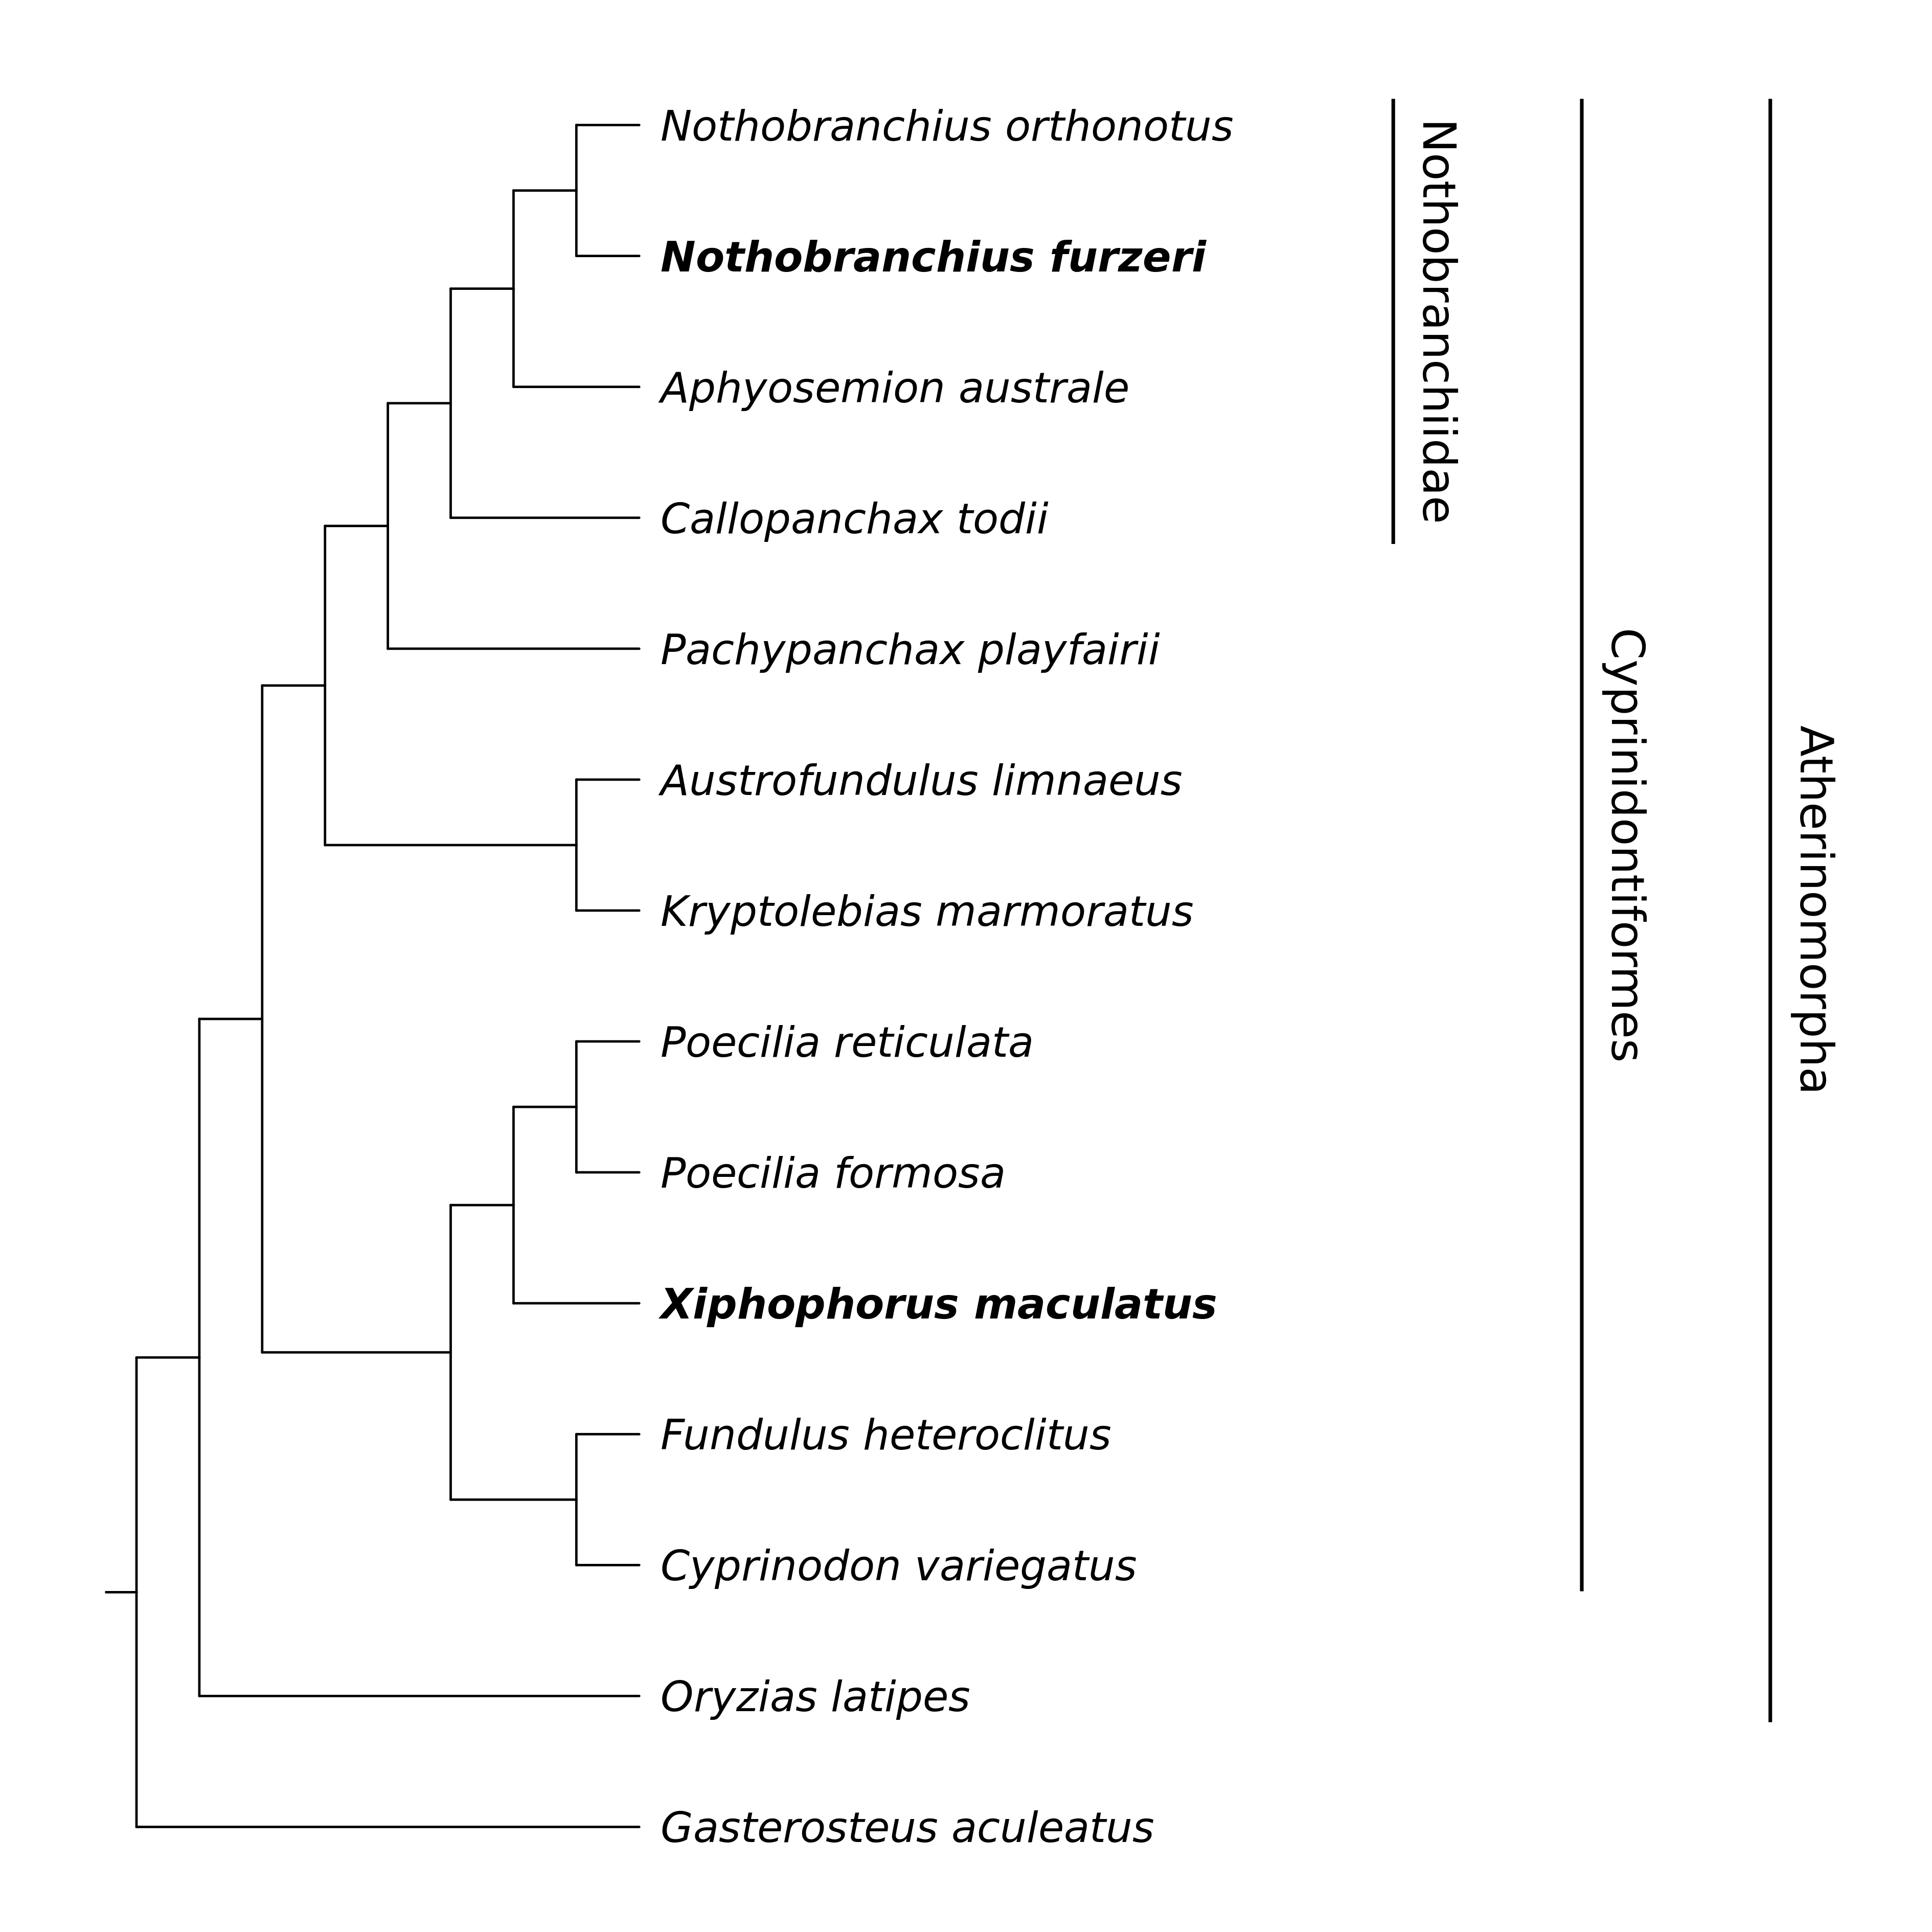
\includegraphics[width=0.9\textwidth]{_Figures/png/species-tree-large-taxa}
	\Caption{Cladogram of species included in the \igh{} locus analysis}{Boldface type indicates species for which new, complete \igh{} locus assemblies were generated for this study; other species were either previously-characterised reference species (\species{G.}{aculeatus}, \species{O.}{latipes}) or underwent constant-region characterisation only (all other species). Labelled vertical bars designate higher taxa of interest.}
	\label{fig:species-tree-large-taxa}
\end{figure}

\section{The \igh{} locus of \nfu}
\label{sec:nfu-locus}

\subsection{Assembling the \Nfu \igh{} locus}
\label{sec:nfu-locus-assembly}

In order to locate and characterise the \nfu \igh{} locus, I collated databases of \vh, \jh, and \ch exon sequences from the published locus sequences of three reference species (zebrafish \parencite{danilova2005zebrafish}, three-spined stickleback \parencite{bao2010stickleback,gambondeza2011stickleback}, and medaka \parencite{magadan2011medaka}, \Cref{sec:methods_comp_locus_reference}) and aligned them to the \nfu genome (NFZ V2.0 \parencite{willemsen2019popgen}) with \program{BLAST} \parencite{altschul1990blast,altschul1997blast}. Genome scaffolds with high-confidence alignments to at least two distinct segment types or covering at least 1\,\% of the scaffold's total length were retained for downstream analysis as potential locus candidates (\Cref{sec:methods_comp_locus_scaffolds}); in total, one chromosome (chr6) and 6 unincorporated scaffolds were identified in this way (\Cref{tab:nfu-locus-scaffolds}), with chromosome 6 bearing the majority of identified gene segments.

\begin{table}[bh]
\centering
\caption{\Nfu genome scaffolds containing putative \igh{} locus fragments}
\begin{threeparttable}
\begin{tabular}{cccccccc}\toprule
\textbf{Scaffold} & \textbf{Total length (kb)} & \textbf{V} & \textbf{J} & \textbf{\cm{}} & \textbf{\cd{}} & \textbf{\cz{}} & Included in locus?\\\midrule
chr6 & 6195.6 & 15 & 7 & 5 & 11 & 0 & Yes\\\midrule
scf10901 & 1.4 & 0 & 0 & 0 & 3 & 0 & Yes\\
scf21863 & 13.5 & 1 & 0 & 0 & 0 & 0 & No\\
scf35954 & 16.3 & 3 & 0 & 0 & 0 & 0 & No\\
scf36277 & 18.9 & 2 & 1 & 0 & 0 & 0 & No\\
scf37083 & 17.7 & 1 & 0 & 0 & 0 & 0 & No\\
scf9157 & 7.2 & 0 & 7 & 4 & 0 & 0 & Yes\\\bottomrule
\end{tabular}

\end{threeparttable}
\label{tab:nfu-locus-scaffolds}
\end{table}

\begin{table}[bh]
\centering
\caption{\Nfu BAC-library inserts containing putative \igh{} locus fragments}
\begin{threeparttable}
\begin{tabular}{cccccccc}\toprule
\textbf{BAC ID} & \textbf{Insert length (kb)} & \textbf{V} & \textbf{J} & \textbf{\cm{}} & \textbf{\cd{}} & \textbf{\cz{}} & Included in locus?\\\midrule
154G24 & 106.6 & 17 & 1 & 0 & 0  & 0 & No\\
162F04 & 119.4 & 5  & 1 & 0 & 0  & 0 & No\\
165M01 & 110.7 & 15 & 1 & 0 & 0  & 0 & Yes\\
206K13 & 106.7 & 17 & 1 & 0 & 0  & 0 & No\\
208A08 & 103.2 & 17 & 1 & 0 & 0  & 0 & Yes\\
209K12 & 133.0 & 1  & 8 & 4 & 20 & 0 & Yes\\
220O06 & 104.8 & 4  & 1 & 0 & 0  & 0 & No\\
223M21 & 99.3  & 17 & 1 & 0 & 0  & 0 & No\\
248A22 & 47.3  & 7  & 0 & 0 & 0  & 0 & No\\
276N03 & 127.9 & 7  & 0 & 0 & 0  & 0 & Yes\\
277J10 & 120.8 & 17 & 1 & 0 & 0  & 0 & Yes\\
\bottomrule\end{tabular}

\end{threeparttable}
\label{tab:nfu-locus-bacs}
\end{table}

In order to determine which of the putative locus scaffolds were in fact part of the \igh{} locus, integrate these into a contiguous locus sequence, and provide additional information on any missing gene segments, I supplemented the locus assembly with insert sequences from bacterial artificial chromosomes in the turquoise-killifish genomic BAC library \parencite{reichwald2015genome}. BAC candidates (whose ends had already been sequenced as part of the genome project) were identified as potentially containing part of the locus sequence (\Cref{sec:methods_comp_bacs_ident}) on the basis of their ends aligning to promising candidate scaffolds from a previous genome assembly (first round) or to the insert sequences of previously sequenced BAC inserts (second round). Once identified,  BAC candidates were isolated from culture by alkaline lysis (\Cref{sec:methods_molec_bacs}), sequenced on an Illumina MiSeq sequencing machine, and assembled and scaffolded with \program{SPAdes} and \program{SSPACE}, respectively (\Cref{sec:methods_comp_bacs_trim,sec:methods_comp_bacs_assembly}). Complete BAC insert assemblies were generated from these scaffolds by manual alignment to overlapping genome scaffolds and other BAC inserts, combined with PCR and Sanger sequencing of intervening sequences.

Having obtained complete insert sequences for promising BAC candidates, I screened them for \igh{} locus segments in the same manner described for genome scaffolds. Passing insert sequences (\Cref{tab:nfu-locus-bacs}) were aligned to and integrated with the identified candidate scaffolds to produce a contiguous locus assembly (\Cref{sec:methods_comp_locus_final}). To minimise the probability of losing relevant gene segments to assembly errors, I gave priority in the event of a sequence conflict between BACs and scaffolds first to any sequence containing a segment missing from the other; if neither the BAC assembly nor the genome scaffolds met this condition, I prioritised the genome scaffold over the BAC assembly. In total, 3 candidate scaffolds (including chromosome 6) and 5 BAC inserts were included in the final locus assembly, while 4 scaffolds and 6 BACs were excluded as likely representing isolated \igh{} orphon segments elsewhere in the genome. The regions of the final locus sequence contributed by different BACs and scaffolds are shown in \Cref{fig:nfu-locus-aln}.

\begin{figure}
\centering
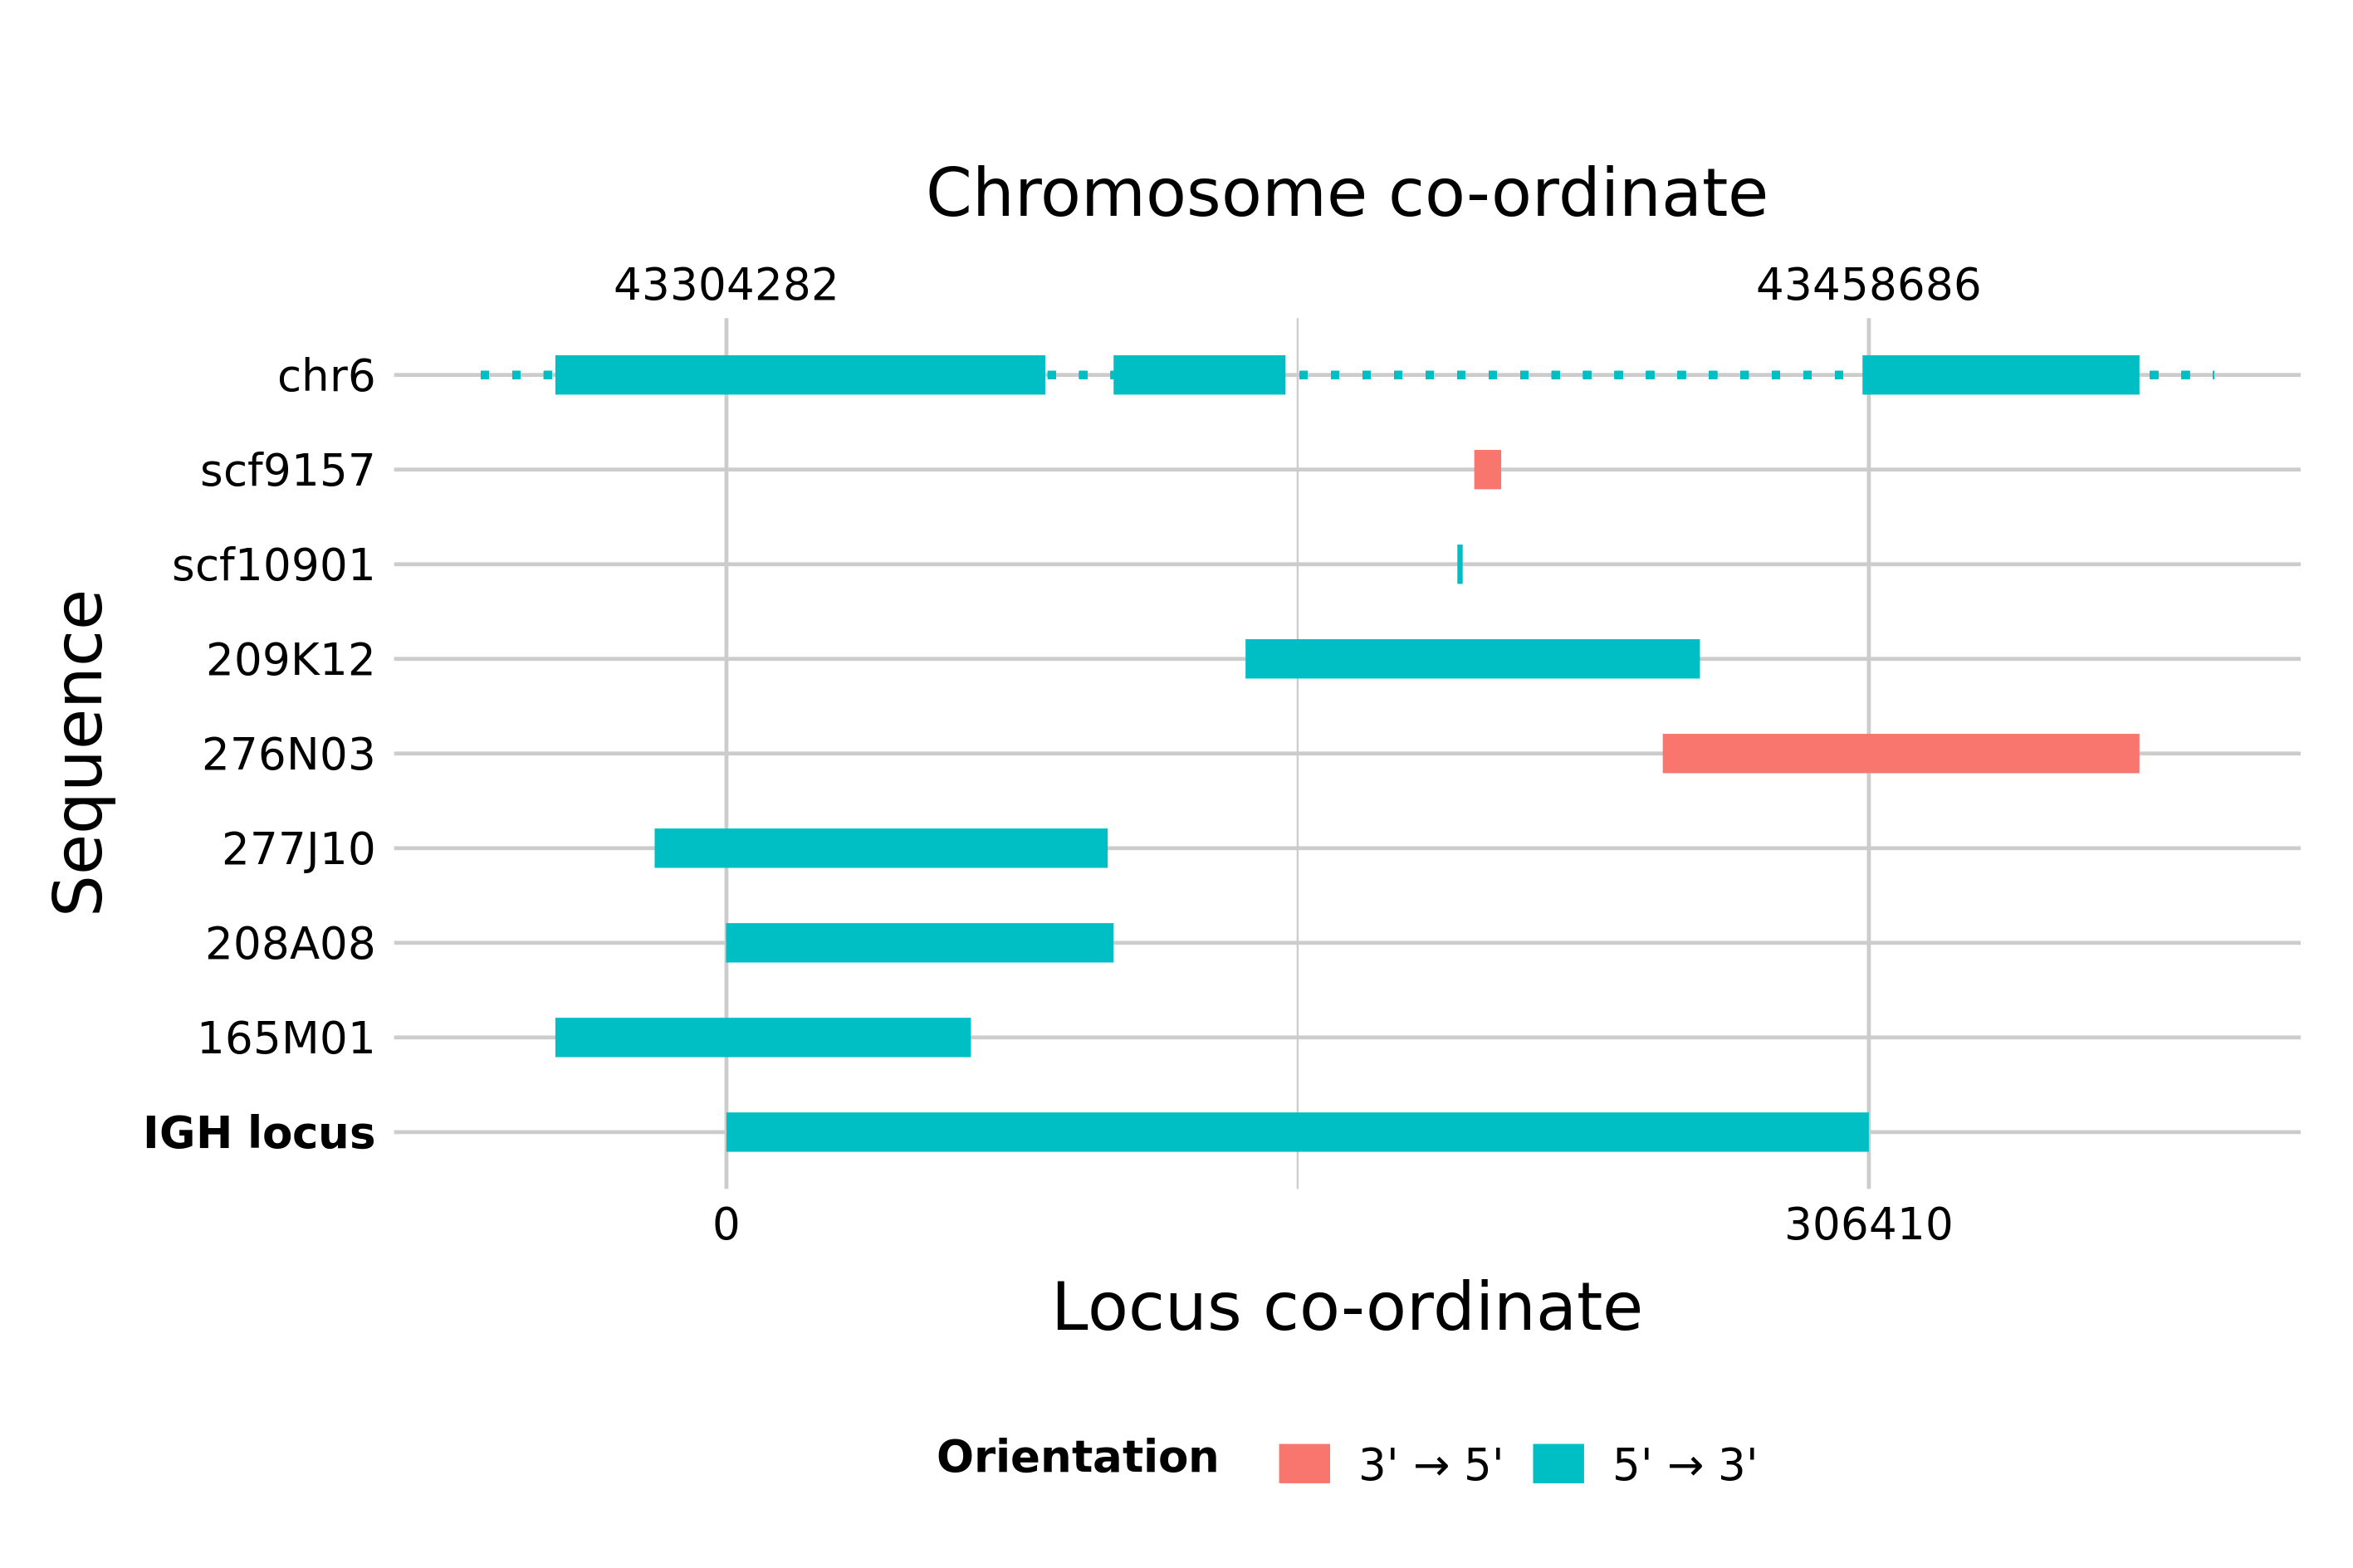
\includegraphics[width=\textwidth]{_Figures/png/nfu-locus-aln}
\Caption{Assembling the \nfu \igh{} locus}{Schematic of genome scaffolds and BAC inserts contributing to the \Nfu \igh{} locus sequence, with their corresponding place within the locus sequence (bottom axis). Internal gaps with dotted lines indicate regions on chromosome 16 with no corresponding locus sequence, as a result of intercalation of BAC or scaffold sequences.}
\label{fig:nfu-locus-aln}
\end{figure}

\subsection{Overall locus structure}
\label{sec:nfu-locus-structure}
	
The turquoise-killifish genome contains a single \igh{} locus approximately 306 kilobases in length, located on chromosome 6 of the \Nfu genome (\Cref{fig:nfu-locus-map-a}). This locus comprises two complete subloci, \igh{1} (\kb{155}) and \igh{2} (\kb{118}), present in tandem and each occupying a classic {\vh-\dh-\jh-\ch} translocon configuration. This modified translocon structure, with multiple translocon subloci present in tandem, has been observed in a number of teleost \igh{} loci including catfish, medaka and stickleback (\Cref{sec:intro_teleost_loci}) \parencite{fillatreau2013astonishing}. Unusually, however, the smaller \igh{2} sublocus in \nfu \igh{} is present in antisense relative to the larger \igh{1}, with the two subloci beginning at opposite ends of the locus and extending in opposite sense towards the middle (\Cref{fig:nfu-locus-map-b}). Such a multi-orientation structure has been seen only rarely in previously-characterised teleost \igh{} loci; to my knowledge, it has only been previously observed in medaka \parencite{magadan2011medaka} and Atlantic salmon (\Cref{fig:intro-teleost-loci-complex}). As medaka is the closest relative of the turquoise killifish to have its locus characterised prior to the present study, it is interesting to see this unusual feature reproduced here, raising the question of whether this ideosyncracy is homologous between the two loci.
	
Compared to other closely-related loci, the turquoise-killifish locus is relatively sparse, with comparatively low functional complexity given its overall size. For example, whereas the stickleback locus fits four subloci, 49 \vh segments and 10 constant regions into c. \kb{200} \parencite{bao2010stickleback,gambondeza2011stickleback}, the turquoise-killifish locus, despite being roughly 50\,\% longer, contains only two subloci, four constant regions and 24 \vh segments (including pseudogenised \vh{}s). This difference is a consequence of the unusually large amount of nonfunctional sequence padding the turquoise-killifish locus, resulting in large gaps between variable segments and in some cases between constant-region exons (\Cref{fig:nfu-locus-map-b}); this high prevalence of repetitive DNA is consistent with the rest of the turquoise-killifish genome, which comprises more than 60\,\% repetitive sequence \parencite{willemsen2019popgen}, compared to just over 15\,\% in stickleback \parencite{yuan2018repeats}.
	
The two subloci in the turquoise-killifish locus are generally highly similar in their functional sequence, with a high degree of synteny between their functional regions (\Cref{fig:nfu-locus-synteny}). The greatest degree of divergence occurs in the \vh and \dh regions, with what appear to be repeated deletion events in \igh{2} resulting in a substantially lower number of \vh and \dh segments compared to \igh{1}; conversely, the \jh and constant regions are almost identical between two subloci. These patterns are discussed in more detail in \Cref{sec:nfu-locus-constant,sec:nfu-locus-variable}.
	
\begin{figure}
	\centering
	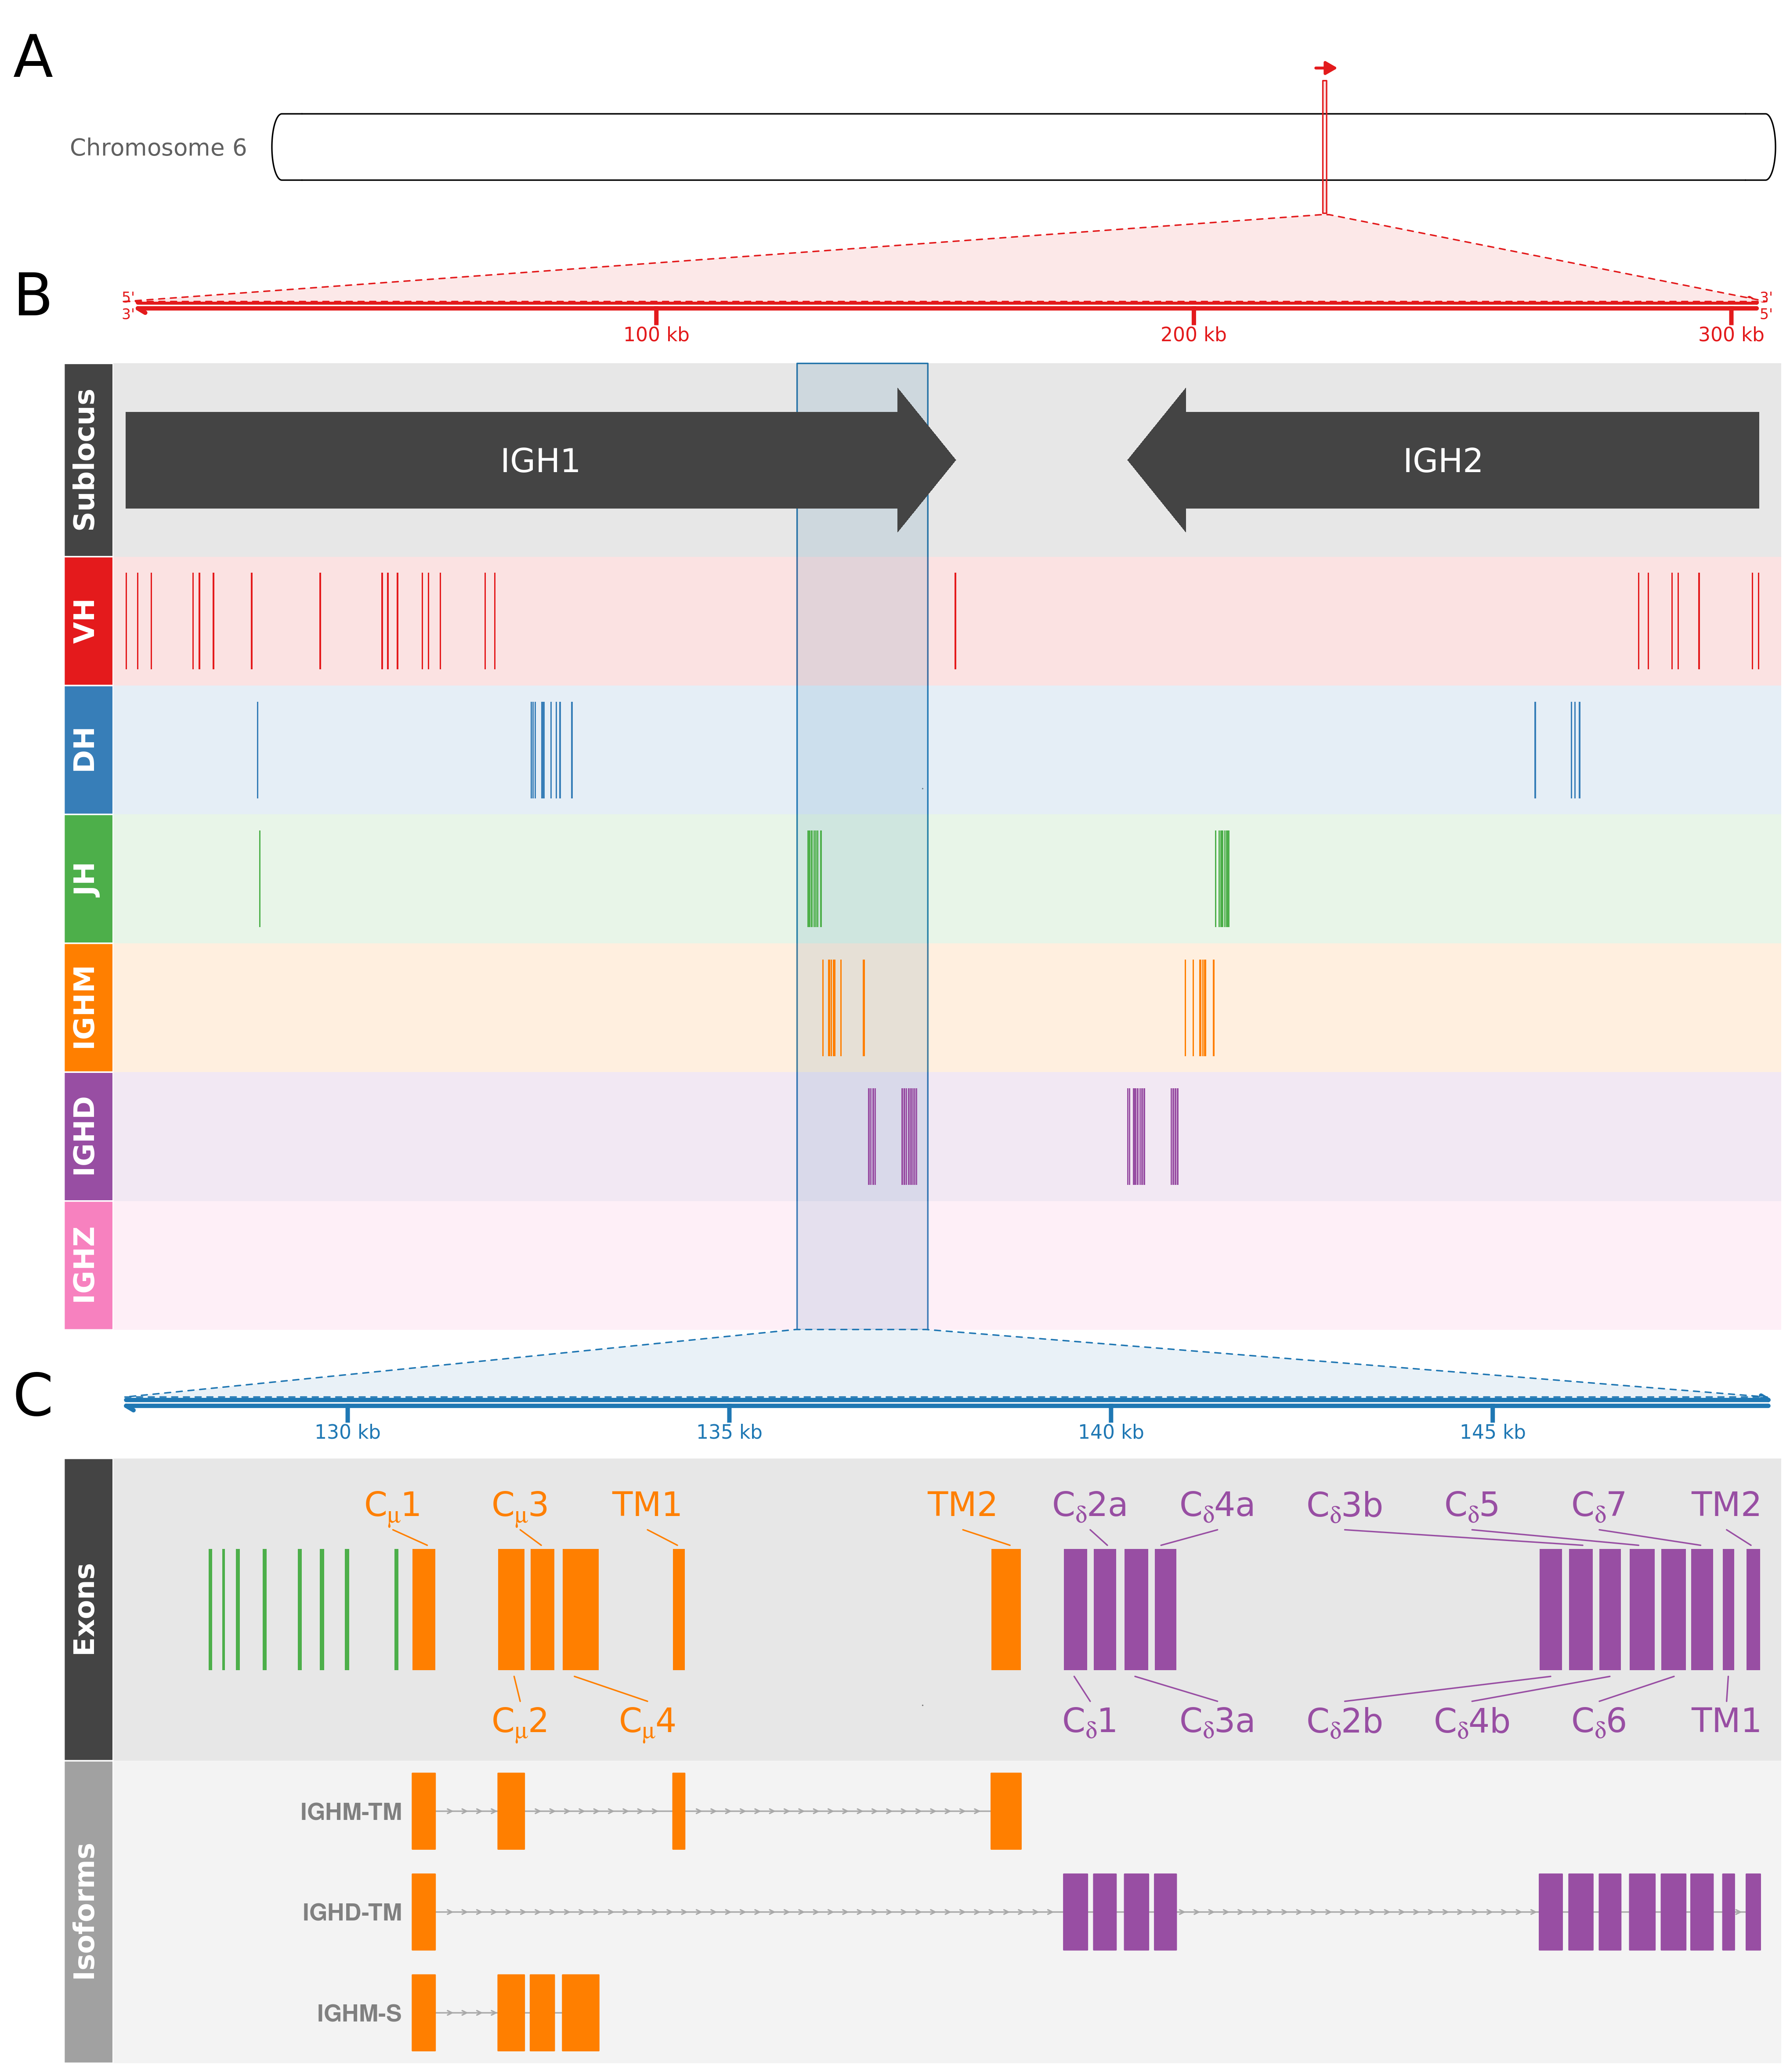
\includegraphics[width=\textwidth]{_Figures/png/nfu-locus-map}
			    \begin{subfigure}{0em}
        \phantomsubcaption{}
        \label{fig:nfu-locus-map-a}
    \end{subfigure}
    \begin{subfigure}{0em}
        \phantomsubcaption{}
        \label{fig:nfu-locus-map-b}
    \end{subfigure}
    \begin{subfigure}{0em}
        \phantomsubcaption{}
        \label{fig:nfu-locus-map-c}
        \end{subfigure}
	\Caption{The immunoglobulin heavy chain (\igh{}) locus in \nfu}{(A) Position of the \igh{} locus on chromosome 6 of the \Nfu genome. (B) Arrangement of \vh, \dh, \jh and constant-region gene segments on the \Nfu \igh{} locus. All segments follow the orientation of their parent sublocus, indicated in the uppermost track. (C) Detailed map of the constant regions of the \igh{1} sublocus, indicating the position and identity of the constant-region exons and the exon composition of expressed \igh{} isoforms in the turquoise killifish.}
	\label{fig:nfu-locus-map}
	\end{figure}
	
\begin{figure}
	\centering
	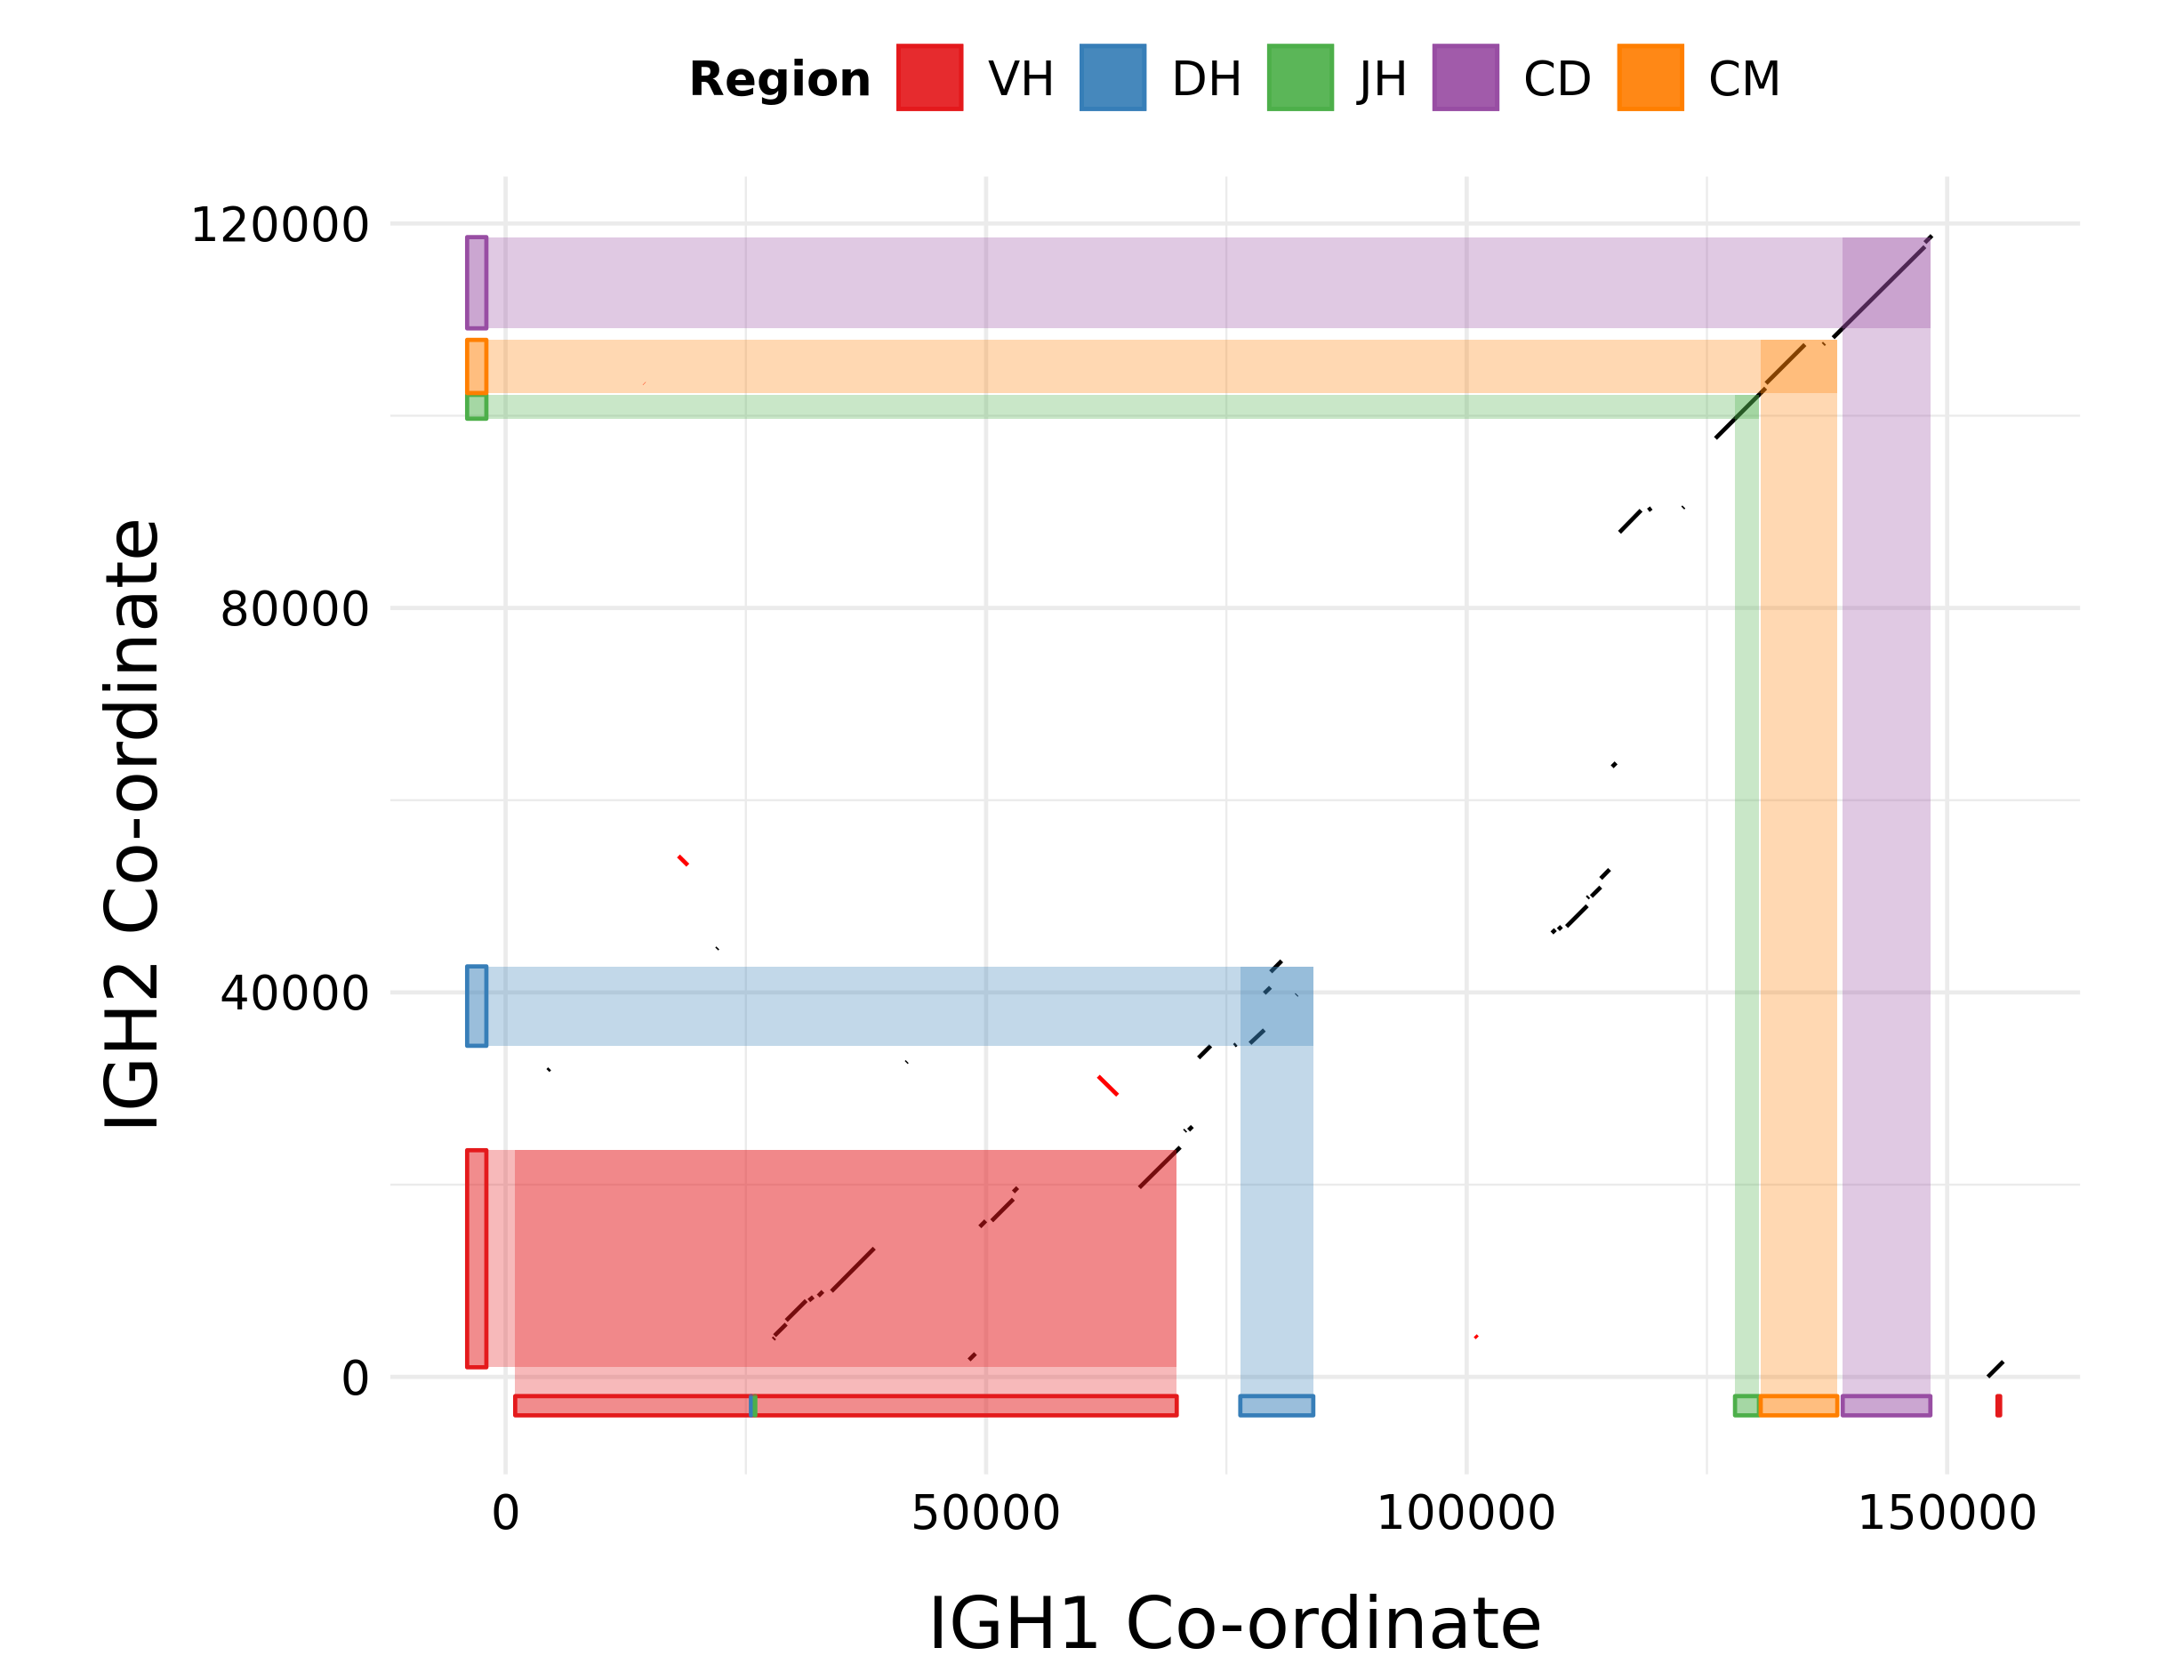
\includegraphics[width=0.9\textwidth]{_Figures/png/nfu-locus-dots}
	\Caption{Sequence homology between subloci in \Nfu \igh{}}{Synteny dot plot of sequential best matches between \igh{1} and \igh{2} subloci, with gene segment regions indicated by coloured rectangles along each axis.}
	\label{fig:nfu-locus-synteny}
\end{figure}
	
	\subsection{Constant regions}
	\label{sec:nfu-locus-constant}
	
	The isotype of an antibody determines its functional role within the immune system, including its possible effector functions and whether it can be secreted (\Cref{sec:intro_antibody_structure}) \parencite{schroeder2010immunoglobulins}. Three antibody isotypes have been identified to date in teleost fishes: \igh{M}, \igh{D} and \igh{Z} (a.k.a. \igh{T}, \igh{T/Z} or \igh{Z/T}) \parencite{fillatreau2013astonishing,bengten2015fishantibodies,magadan2015fishrepertoires}. Of these, \igh{M} and \igh{D} are highly primitive within the jawed vertebrates and found in most or all other vertebrate groups; within the teleosts, both appear to be universal \parencite{bengten2015fishantibodies}. Conversely, \igh{Z} is a teleost-specific isotype which is absent in other vertebrate taxa; within the teleosts, most characterised \igh{} loci possess \igh{Z}, but at least two (medaka and channel catfish) have been found to lack it \parencite{fillatreau2013astonishing,bengten2015fishantibodies}. In rainbow trout, \igh{Z} has been found to play a specialised mucosal role in the immune system analagous to that of \igh{A} in mammals \parencite{zhang2010igtgut,xu2013igtskin}, and it is widely assumed to play this specialised role throughout the teleosts; it is as yet unclear how mucosal immunity is effected in species lacking \igh{Z} (\Cref{sec:intro_antibody_structure}).

In order to investigate constant regions in the \nfu \igh{} locus, I identified putative exon sequences using \program{BLAST} alignments to the reference sequence databases described in \Cref{sec:nfu-locus-assembly}. Intron/exon bounderies were refined through alignment of published RNA-sequencing data from turquoise-killifish gut (\parencite{smith2017microbiota}, BioProject accession PRJNA379208, young and old untreated groups, \Cref{tab:rnaseq-sources}) using \program{STAR} (\Cref{sec:methods_comp_locus_segments} and \Cref{fig:nfu-locus-sashimi}). Strikingly, the \nfu \igh{} locus appears to completely lack any \igh{Z} constant region, with no \cz{} exons or \igh{Z} transmembrane exons being found on either \igh{1} or \igh{2}. Given the widespread prevalence and specialised mucosal role of \igh{Z} in teleosts, its surprising absence in turquoise killifish (\Cref{fig:nfu-locus-map-b}) immediately raises questions about the nature, kinetics and efficacy of mucosal adaptive immunity in this species. The similar absence of \igh{Z} in medaka, which again is the closest relative of \Nfu with a characterised locus, raises further questions about the evolutionary history of \igh{Z} in these species: does the shared absence of \igh{Z} in these species indicate a single ancestral deletion event, or parallel loss of this important isoform within both the Cyprinodontiformes (including the turquoise killifish) and the lineage leading to medaka? This latter question requires higher phylogenetic resolution to address effectively, and is investigated further in \Cref{sec:xma-locus} and \Cref{sec:locus_comparative}.
	
	While \igh{Z} is completely missing from the \Nfu \igh{} locus, \igh{M}, the most primitive and widely-found isotype in jawed vertebrates, is present in its expected location immediately downstream of the main \jh-region in both subloci. This constant region occupies the standard six-exon configuration, with four \cm{} exons and two transmembrane exons present in series on the chromosome (\Cref{fig:nfu-locus-map-b,fig:nfu-locus-map-c,fig:teleost-igm-exons-a}, \Cref{tab:nfu-ch-coords}). As with other species, both secreted and transmembrane isoforms of \igh{M} are present in the transcriptome, with secreted \igh{M} (\igh{M-S}) consisting of \cm{1-4} (\Cref{fig:nfu-locus-map-c,fig:nfu-locus-sashimi-a,fig:teleost-igm-exons-b}); however, the exon configuration of transmembrane \igh{M} (\igh{M-TM}) deviates from both that seen in mammals (in which exon TM1 is spliced to a cryptic splice site within \cm{4}) and most teleosts (in which the canonical splice site following \cm{3} is used and \cm{4} is excised) \parencite{fillatreau2013astonishing}. Rather, turquoise-killifish \igh{M-TM} resembles that of medaka, in which both \cm{3} and \cm{4} are excluded and the canonical splice site at the end of \cm{2} is spliced directly to TM1 (\Cref{fig:teleost-igm-exons-c,fig:teleost-igm-exons-d,fig:teleost-igm-exons-e}). This similarity to medaka again raises the possibility that this unusual feature may be a conserved feature of both lineages; however, the underlying mechanism giving rise to this difference in splicing behaviour is unknown.
	
		Unlike \igh{M}, the exon structure of \igh{D} is highly variable across the teleosts, ranging from roughly 7-17 \cd{} exons in addition to the transmembrane domains \parencite{fillatreau2013astonishing}. The core structure of \igh{D} comprises seven \cd{} exons (\cd{1-7}), but some subset of these exons may be missing or duplicated in any given species -- in medaka, for example, \cd{5} is missing in all subloci \parencite{magadan2011medaka}, while in many species (e.g. zebrafish, salmon, and channel catfish) \cd{2-4} are duplicated in two or more tandem blocks \parencite{fillatreau2013astonishing}. This latter configuration is also observed in turquoise killifish, in which the \igh{D} constant region immediately follows \igh{M} in both subloci and has a 

\cd{1}-(\cd{2}-\cd{3}-\cd{4})$_2$-\cd{5}-\cd{6}-\cd{7}-TM1-TM2 

	\noindent configuration, for a total of 12 exons per \igh{D} constant region (\Cref{fig:nfu-locus-map-b,fig:nfu-locus-map-c}, \Cref{tab:nfu-ch-coords}). All of these exons appear to be expressed in tandem, resulting in a much longer transcript than is observed for any isoform of \igh{M} (\Cref{fig:nfu-locus-map-c,fig:nfu-locus-sashimi-b}). As in other teleost species, \igh{D} in the turquoise killifish includes a chimeric \cm{1} exon at the 5' end of the constant-region transcript, for a total of 13 exons per \igh{D-TM} mRNA (\Cref{fig:nfu-locus-sashimi-b}).

	While the best-known form of \igh{D} in teleosts is transmembrane, secreted \igh{D} has been observed in at least two teleost species, with different mechanisms used in each case: in channel catfish, one dedicated sublocus has a dedicated \igh{D} secretory exon in place of the transmembrane exons \parencite{bengten2006catfish}, while in rainbow trout (and possibly some other species like Atlantic salmon and cod \parencite{ramirezgomez2012secretoryigd}) a run-on event at the end of \cd{7} results in the production of a secretory tail in a manner similar to secretory \igh{Z} \parencite{ramirezgomez2012secretoryigd}. However, neither a specialised secretory exon nor a \cd{7} secretory tail could be detected in turquoise killifish, suggesting that \igh{D} may only be expressed in transmembrane form in this species.
	
	In the case of both \igh{M} and \igh{D}, the constant regions are present in their expected configuration in each sublocus and are highly similar in sequence between the subloci, with an average of 98.4\,\% nucleotide sequence identity for corresponding \igh{M} exons and 99.3\,\% for corresponding \igh{D} exons (\Cref{fig:nfu-ch-aln} and \Cref{tab:nfu-ch-aln}) in pairwise Needleman-Wunsch alignments \parencite{needleman1970alignment}. This high level of similarity indicates either a very recent duplication event to produce the second sublocus or a high level of sequence conservation in both subloci, with the latter explanation suggesting that both subloci continue to be functional and active in the immune system.
	
	\begin{figure}
	\centering
		    \begin{subfigure}{0em}
        \phantomsubcaption{}
        \label{fig:teleost-igm-exons-a}
    \end{subfigure}
    \begin{subfigure}{0em}
        \phantomsubcaption{}
        \label{fig:teleost-igm-exons-b}
    \end{subfigure}
    \begin{subfigure}{0em}
        \phantomsubcaption{}
        \label{fig:teleost-igm-exons-c}
    \end{subfigure}
    \begin{subfigure}{0em}
        \phantomsubcaption{}
        \label{fig:teleost-igm-exons-d}
    \end{subfigure}
    \begin{subfigure}{0em}
        \phantomsubcaption{}
        \label{fig:teleost-igm-exons-e}
    \end{subfigure}
	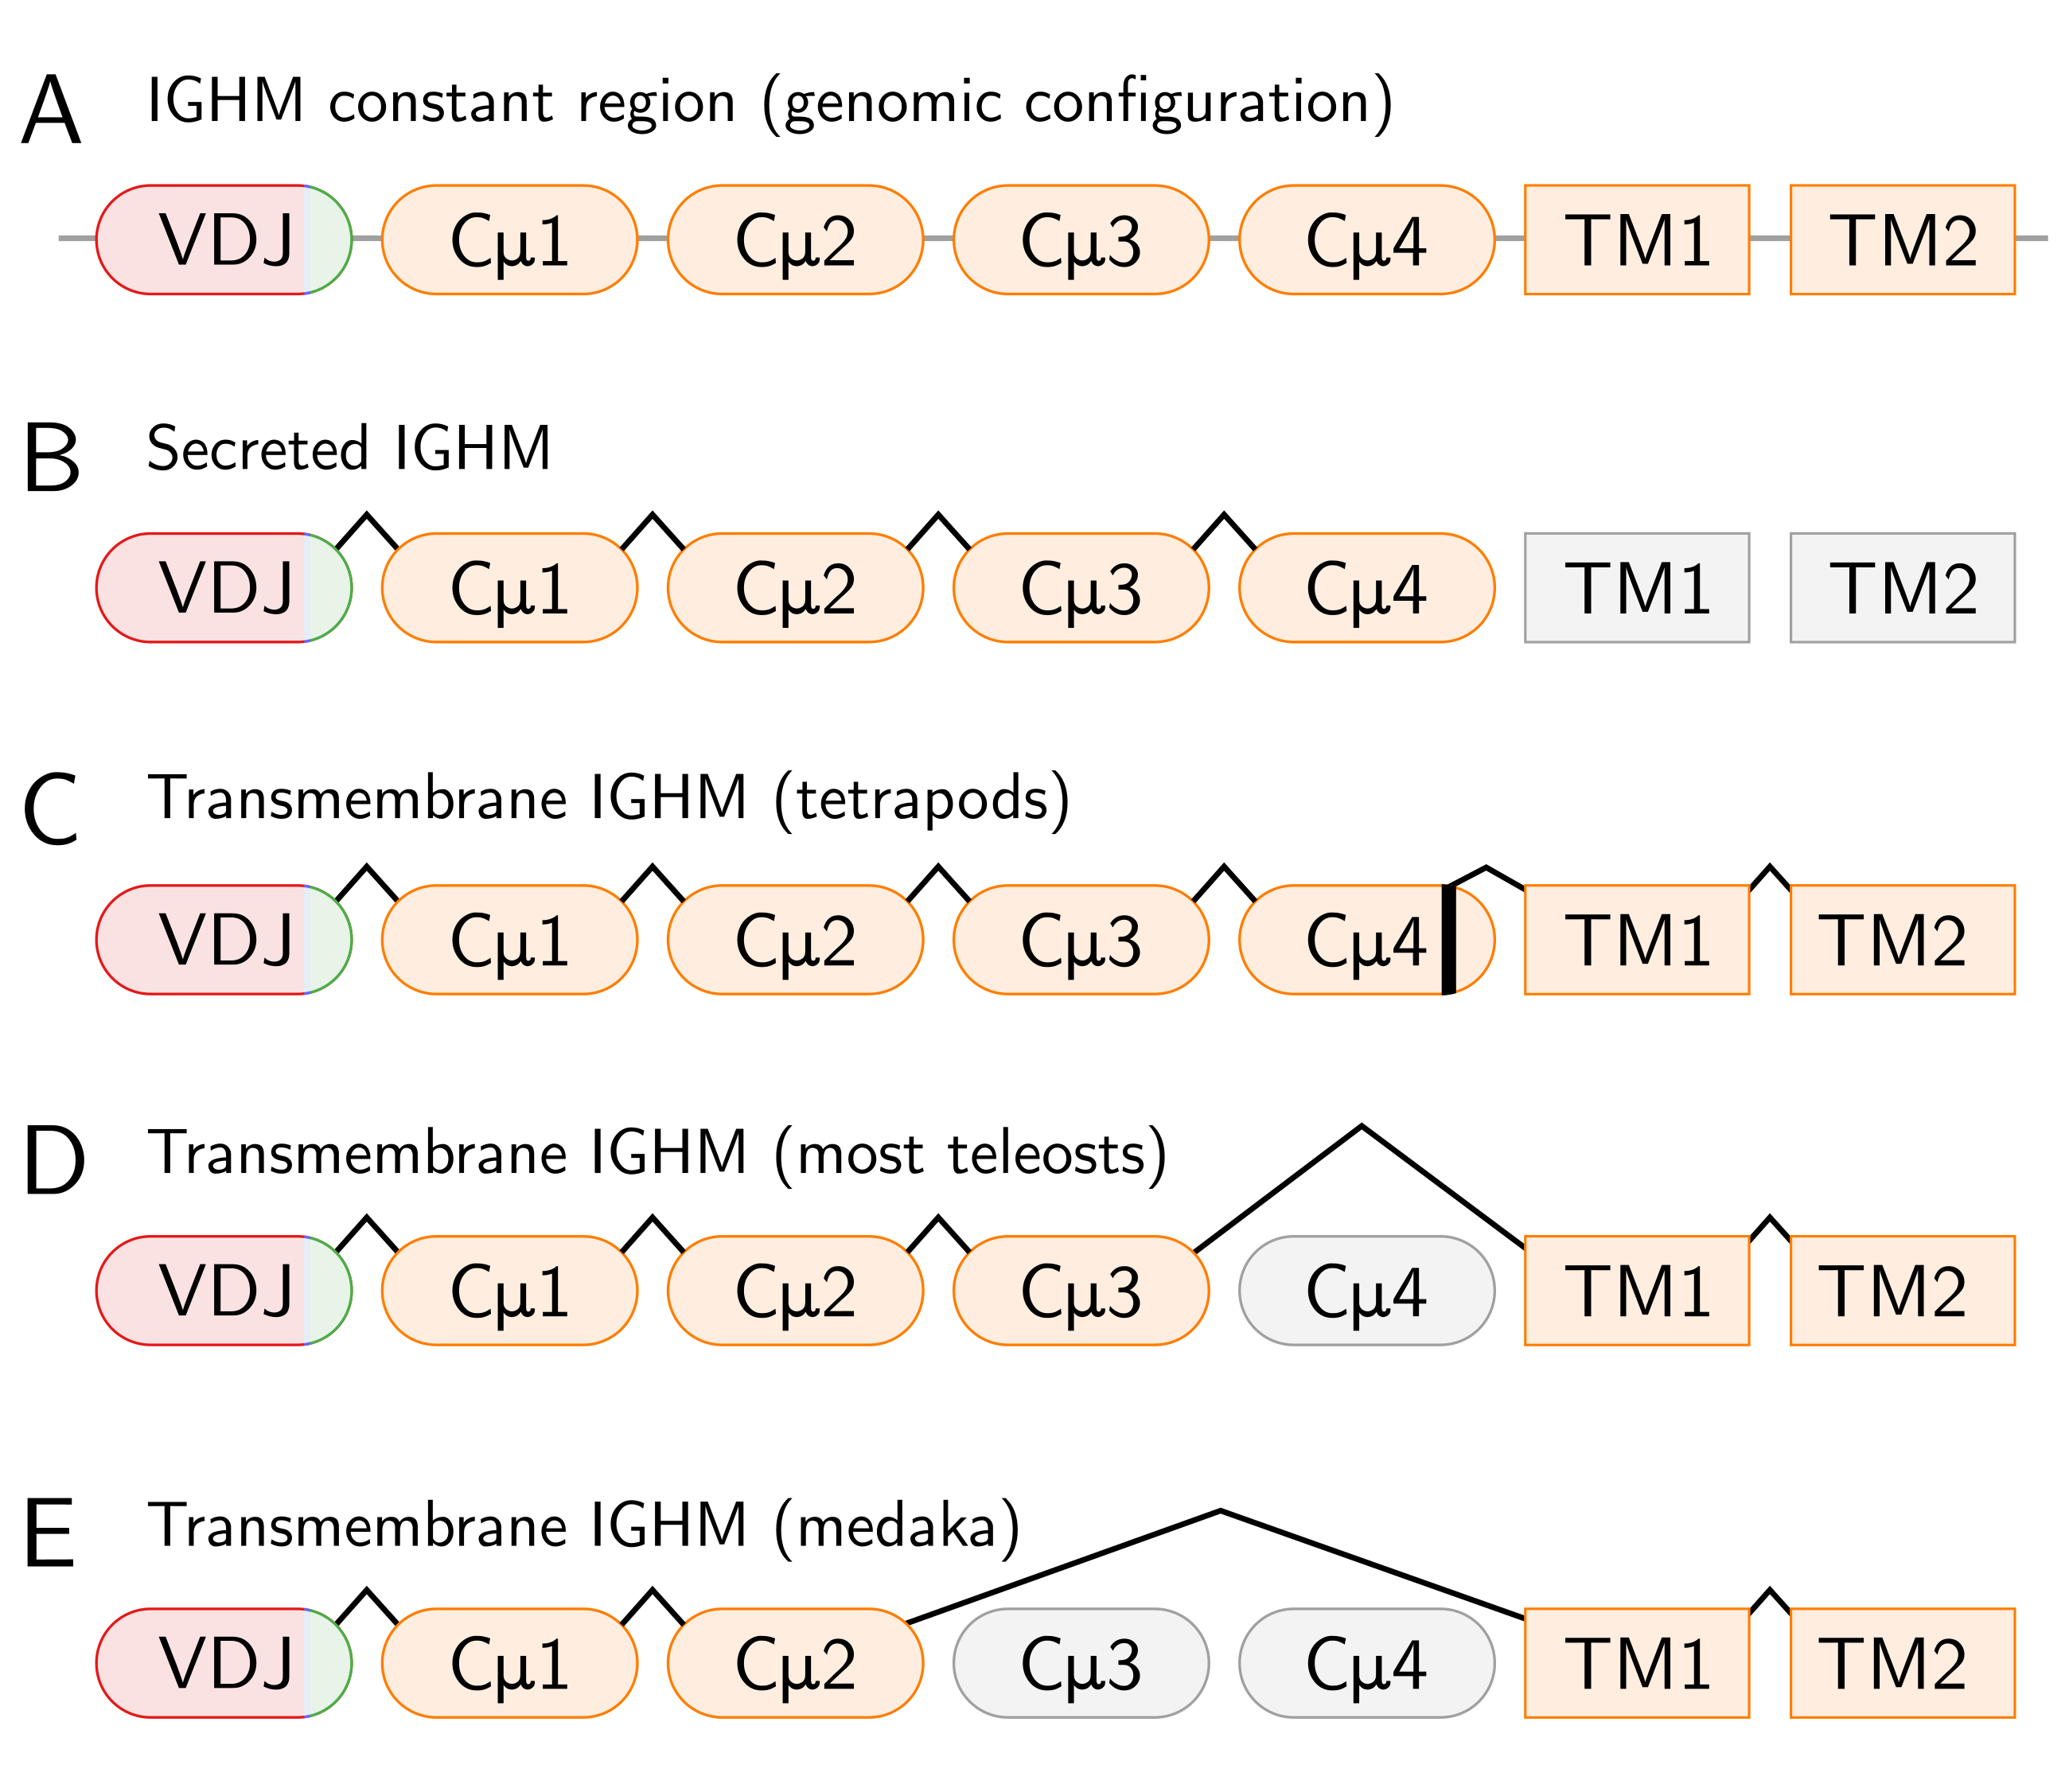
\includegraphics[width=0.8\textwidth]{_Figures/png_edited/teleost-igm-exons}
	\Caption{\igh{M} exon usage in bony vertebrates}{Schematic of \igh{M} splice patterns in different isoforms and taxonomic groups; (A) standard genomic (pre-splicing) configuration of \igh{M}, following VDJ recombination; (B) exon configuration of secreted \igh{M} (\igh{M-S}) in tetrapods and teleosts; (C) exon configuration of transmembrane \igh{M} (\igh{M-TM}) in tetrapods, demonstrating the use of a cryptic splice site in \cm{4}; (D) standard \igh{M-TM} exon configuration in teleosts, demonstrating the direct splicing of \cm{3} to TM1 and exclusion of \cm{4}; (E) unusual \igh{M-TM} exon configuration observed in medaka, in which both \cm{3} and \cm{4} are excluded. Adapted from Figure 3 of \parencite{fillatreau2013astonishing}.}
	\label{fig:teleost-igm-exons}
	\end{figure}
	
	\begin{figure}
	\centering
		\begin{subfigure}{0em}
        \phantomsubcaption{}
        \label{fig:nfu-locus-sashimi-a}
    \end{subfigure}
    \begin{subfigure}{0em}
        \phantomsubcaption{}
        \label{fig:nfu-locus-sashimi-b}
    \end{subfigure}
	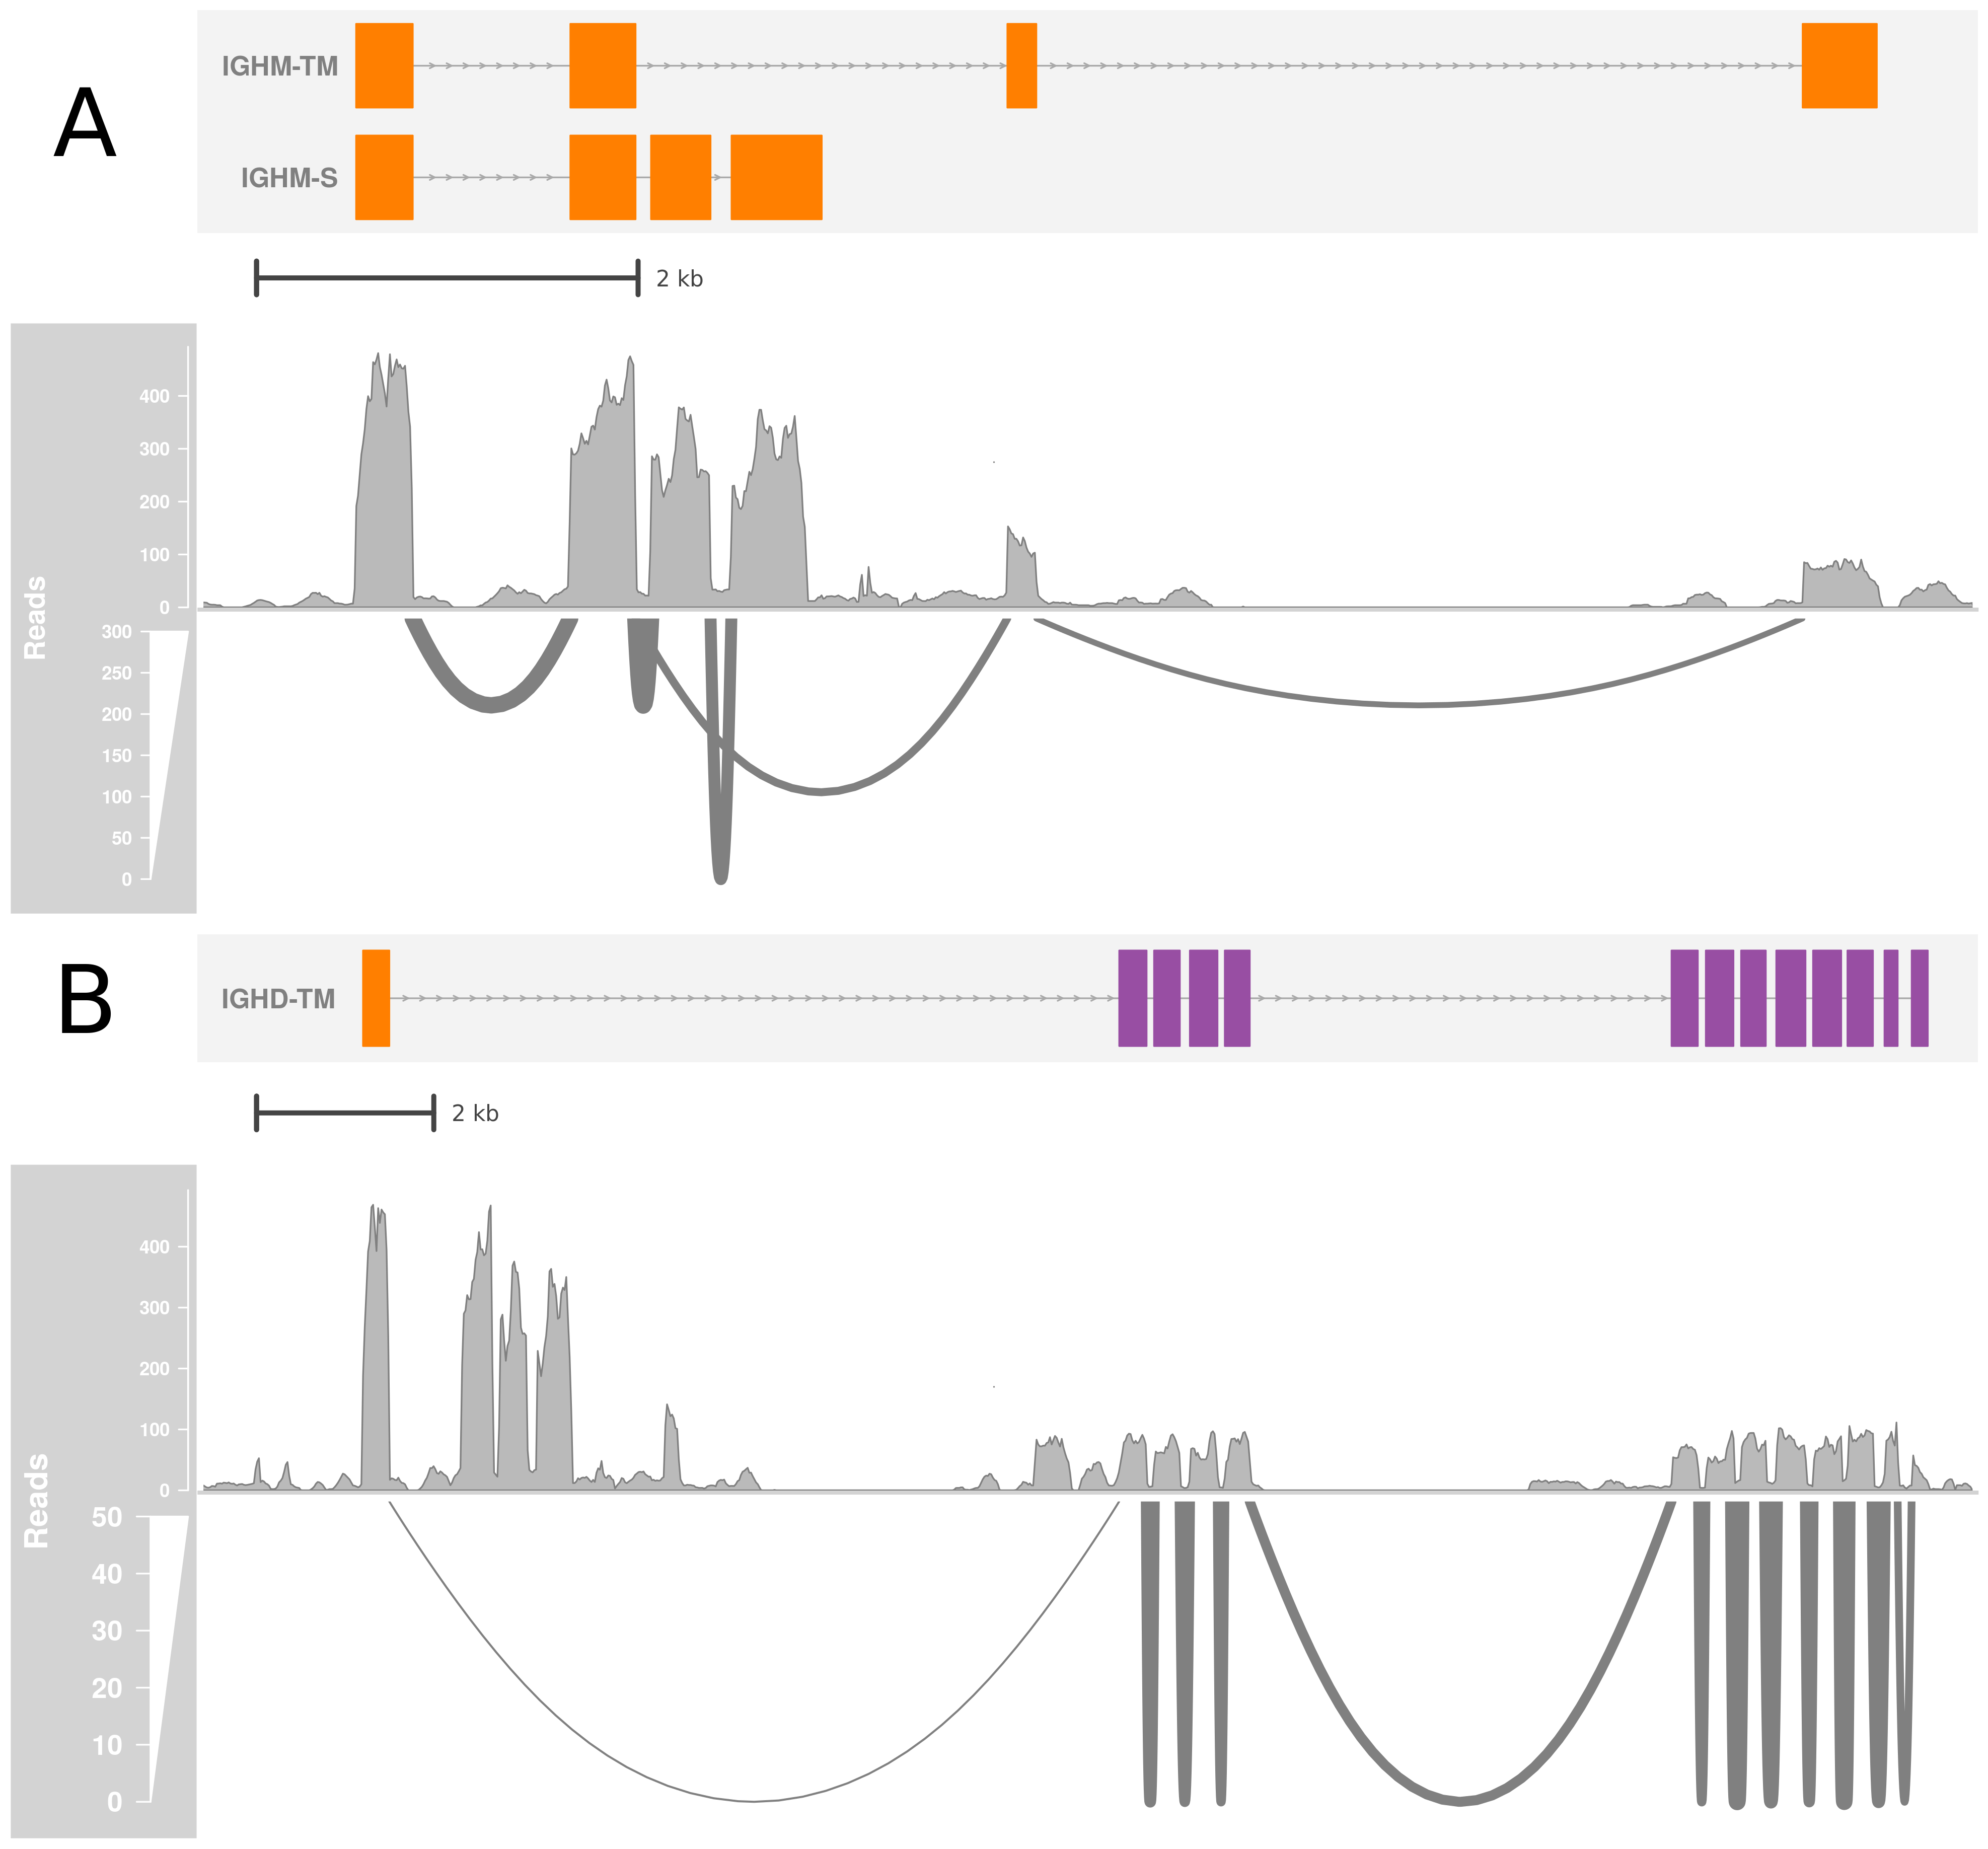
\includegraphics[width=\textwidth]{_Figures/png/nfu-locus-sashimi}
	\Caption{Constant-region isoforms in \Nfu}{Coverage and Sashimi plots \parencite{katz2013sashimi} of \program{STAR}-aligned RNA-seq reads from \Nfu gut samples \parencite{smith2017microbiota}, demonstrating the splicing behaviour of \igh{1} constant-region isoforms and showing the read coverage of each exon and splice junction. (A) \igh{M} exon splicing, showing alternative splicing patterns of \igh{M-TM} and \igh{M-S}; (B) \igh{D} exon splicing, showing chimeric splicing of \cm{1} to \cd{1}.}
	\label{fig:nfu-locus-sashimi}
	\end{figure}
	
	\begin{figure}
	\centering
	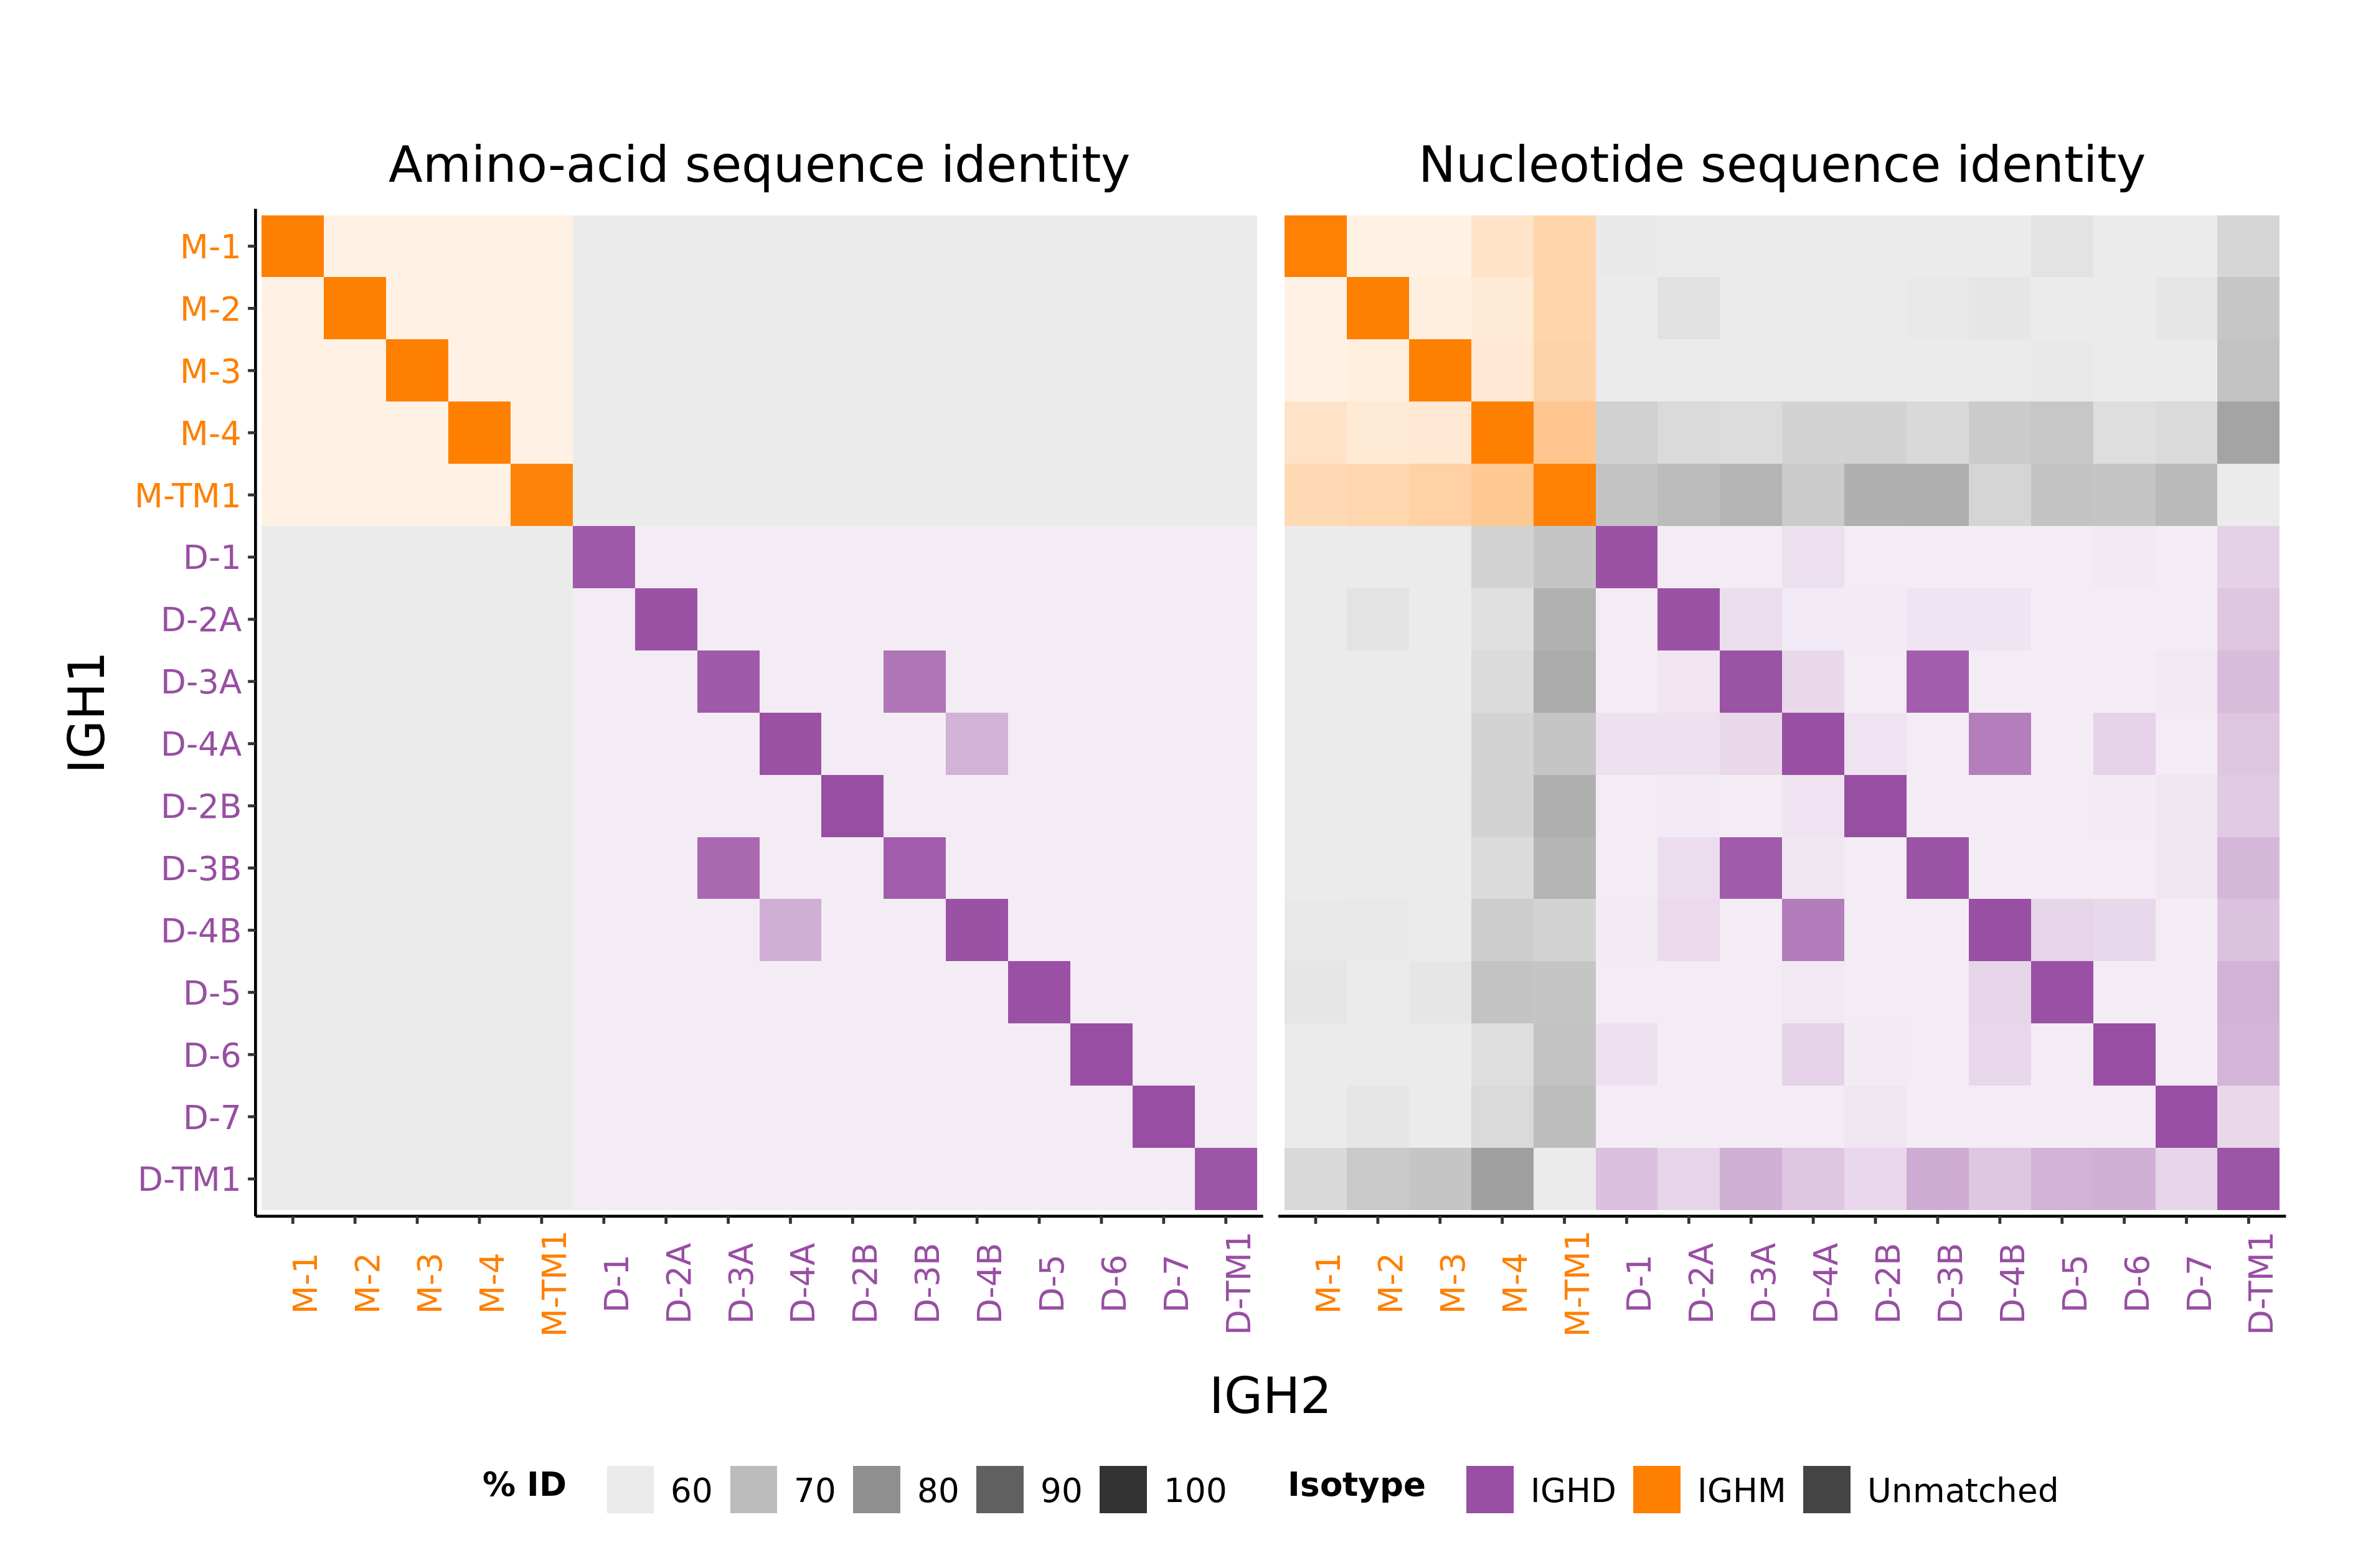
\includegraphics[width = \textwidth]{_Figures/png/nfu-ch-aln}
	\Caption{Cross-sublocus sequence similarity of constant-region exons in \Nfu \igh{}}{Heatmap of percentage sequence identity between amino-acid (left) and nucleotide (right) sequences of constant-region exons (excluding \igh{M-TM2} and \igh{D-TM2}) from the two subloci of \Nfu \igh{}, calculated using pairwise Needleman-Wunsch global alignments.}
	\label{fig:nfu-ch-aln}
	\end{figure}
	
	\begin{table}\centering
		\Caption{Cross-sublocus sequence similarity of constant-region exons in \Nfu}{Percentage sequence identities of pairwise Needleman-Wunsch global alignments between nucleotide (NT) or amino-acid (AA) sequences of corresponding exons from the two subloci of \Nfu \igh{}.}
	% latex table generated in R 3.5.1 by xtable 1.8-3 package
% Wed Dec 19 17:33:43 2018
\begin{tabular}{llrr}
  \toprule Isotype & Exon & NT & AA \\ 
  \midrule M & 1 & 99.66 & 100.00 \\ 
  M & 2 & 100.00 & 100.00 \\ 
  M & 3 & 100.00 & 100.00 \\ 
  M & 4 & 100.00 & 100.00 \\ 
  M & TM1 & 99.34 & 98.00 \\ 
  M & TM2 & 91.67 & 100.00 \\ 
  D & 1 & 99.03 & 97.06 \\ 
  D & 2A & 98.97 & 98.96 \\ 
  D & 3A & 98.72 & 97.09 \\ 
  D & 4A & 99.65 & 98.92 \\ 
  D & 2B & 100.00 & 100.00 \\ 
  D & 3B & 98.72 & 96.12 \\ 
  D & 4B & 99.64 & 98.91 \\ 
  D & 5 & 99.09 & 99.08 \\ 
  D & 6 & 100.00 & 100.00 \\ 
  D & 7 & 100.00 & 100.00 \\ 
  D & TM1 & 97.99 & 97.96 \\ 
  D & TM2 & 99.44 & 100.00 \\ 
   \bottomrule \end{tabular}

	\label{tab:nfu-ch-aln}
	\end{table}
	
\subsection{Variable regions}
\label{sec:nfu-locus-variable}
	
Variable-region gene segments in the turquoise-killifish \igh{} locus were identified with a variety of methods, depending on the type of gene segment being analysed (\Cref{sec:methods_comp_locus_segments}). \vh candidates were identified probabilistically using Hidden Markov Models constructed by \program{nhmmer} \parencite{wheeler2013nhmmer} from \program{PRANK} \parencite{loytynoja2014prank} multiple-sequence alignments of reference sequences, with the 3'-ends of each V-exon identified by the presence of a recombination-signal sequence (RSS) \parencite{schroeder2010immunoglobulins} and the 5'-ends refined using \program{IMGT-DomainGapAlign} \parencite{ehrenmann2011domaingapalign}. \jh candidates were also identified using \program{nhmmer}, with segment ends identified by the presence of an RSS (5') and a \sequence{GTA} splice-site motif (3') \parencite{magadan2011medaka}. Finally, \dh-segments, being too short and variable in sequence for HMM-based approaches to be effective, were identified by searching for pairs of flanking RSS sequences in opposite orientation, using fuzzy pattern-matching (with EMBOSS \program{FUZZNUC} \parencite{rice2000emboss}) to conserved RSS sequence motifs.
	 
In total, I identified 24 \vh-segments, 14 \dh-segments and 17 \jh-segments in the \Nfu locus (\Cref{tab:nfu-vh-coords,tab:nfu-dh-coords-seg,tab:nfu-jh-coords-seg}), of which the majority (17 \vh, 10 \dh and 8 \jh) were present in \igh{1}. Of the \vh segments identified, three contain premature stop codons, though none is out-of-frame; conversely, all the \dh and \jh segments identified appear to be in-frame and functional, with no premature stop codons. However, in all cases a minority of segments contain RSS sequences that deviate significantly from the expected consensus sequence (\Cref{tab:nfu-vh-coords,tab:nfu-dh-coords-rss5,tab:nfu-dh-coords-rss3,tab:nfu-jh-coords-rss}); it is unclear whether these sequences can recombine to successfully produce mature VDJ sequences \textit{in vivo}. In the case of the \vh segments, of the six sequences without clearly functional RSS sequences, three also contain premature stop codons, suggesting the changes to the RSS in these cases may arise from relaxed purifying selection on already-pseudogenised sequences.

Apart from these few exceptions, however, the recombination signal sequences (RSS) marking the ends of the \vh, \dh and \jh gene segments in the \Nfu locus otherwise strongly resemble those of other characterised teleosts, which in turn resemble those of non-teleost loci (\Cref{fig:nfu-rss-seqlogo-all,fig:nfu-rss-seqlogo-sep}). The overall heptamer and nonamer consensus sequences (\texttt{CACAGTG} for heptamers and \texttt{ACAAAAACC} for nonamers) closely matched those expected from the literature \parencite{schroeder2010immunoglobulins}, while in 88\,\% of cases the spacer region was within 1bp of the expected length (12bp for \dh-RSSs, 23bp for \vh- and \jh-RSSs); interestingly, the greatest number of \vh-RSSs had a 22bp (rather than 23bp) spacer, but this is unlikely to interfere with RSS functionality. Overall, the RSSs in the turquoise killifish appear to be supporting the normal operation of VDJ-recombination in this species.

Of the \vh, \dh and \jh segments identified, all but one of each type of segment is located within contiguous V-, D-, and J-regions within each sublocus, supporting a modified translocon configuration for turquoise-killifish \igh. The exceptions to this are \igh{1D01} and \igh{1J01}, which are embedded within the \igh{1} V-region, and a single \vh segment located in between the \igh{D} constant regions of the two subloci (\Cref{fig:nfu-locus-map-b}). The unusual location of \igh{1D01} and \igh{1J01} may represent the result of a transposition event within the \igh{} locus; however, their close colocalisation and 5' position within the \igh{1} sublocus, as well as the fact that neither has a close paralogue in \igh{2} (\Cref{fig:nfu-dj-alignment-b}), suggest that they may instead represent the remnant of a formerly present \igh{Z} constant region, as these typically have dedicated D/J segments independent of those serving \igh{M} (\Cref{sec:intro_teleost_loci}). Given its forward orientation, meanwhile, I assigned the orphaned \vh-segment to the \igh{1} sublocus as \igh{1V1-07}; however, if annotated correctly, it is unlikely to successfully recombine with segments in either sublocus due to its unusual location.
		
\begin{table}[hb]
	\centering
	\begin{threeparttable}
	\centering
	\caption{Number of functional \vh-segments and \vh-families in other teleost species}
	\label{tab:teleost-vh-counts}
	\begin{tabular}{ccccc}\toprule
	\multirow{2}{*}{	\textbf{Common Name}} & \multirow{2}{*}{\textbf{Species}} & \textbf{\# Functional} & \textbf{	\# \vh} & \multirow{2}{*}{\textbf{Source}} \\
	& & \textbf{\vh Segments} & \textbf{Families} & \\\midrule
	Zebrafish & \textit{Danio rerio} & 39 & 13\,\tnote{1} & \parencite{magadan2015fishrepertoires} \\
	Grass carp & \textit{Ctenopharyngodon idella} & 8 & 5\,\tnote{2} & \parencite{xiao2010grasscarp} \\
	Fugu & \textit{Takifugu rubripes} & 34 & 3 & \parencite{magadan2015fishrepertoires} \\
	Medaka & \textit{Oryzias latipes} & 35 & 6 & \parencite{fillatreau2013astonishing,magadan2011medaka} \\
	Stickleback & \textit{Gasterosteus aculeatus} & 49 & 4 & \parencite{magadan2015fishrepertoires} \\
	Turquoise killifish & \textit{Nothobranchius furzeri} & 21\,\tnote{3} & 6 & -- \\
	\bottomrule\end{tabular}
	\begin{tablenotes}
	\item[1] \vh families in zebrafish were identified based on 70\,\% (rather than 80\,\%) sequence identity.
	\item[2] It is not clear what clustering method or threshold was used to identify \vh families in grass carp.
	\item[3] Excluding \vh segments with nonsense or frameshift mutations, but not those with uncertain or missing RSS sequences.
	\end{tablenotes}
	\end{threeparttable}
\end{table}
	
\vh sequences within an \igh{} locus are conventionally grouped into families on the basis of nucleotide sequence identity, with a typical identity cutoff of 80\,\% \parencite{magadan2015fishrepertoires}. In order to group the \Nfu \vh genes into families, I performed pairwise Needleman-Wunsch global alignments on each pair of \vh sequences to obtain pairwise identity scores, followed by single-linkage clustering on the resulting identity matrix (\Cref{sec:methods_comp_locus_segments}). Cutting the dendrogram at 80\,\% sequence identity revealed a total of six \vh families, of which four contained more than one \vh segment (\Cref{fig:nfu-vh-families}); this number of \vh families in the \Nfu locus is roughly in line with those found in related species (\Cref{tab:teleost-vh-counts}). Of these, V1 and V2 make up the bulk (42\,\% and 29\,\% respectively) of the \vh segments in the locus. V2 and V4 are highly similar, and all the members of V4 are pseudogenised by premature stop codons; it may therefore be more appropriate to regard V4 as a pseudogenised subfamily of V2 than as a \vh family in its own right.

The total number of functional \vh segments in the turquoise-killifish locus is unusually small in comparison to the total numbers observed in many other teleost species (\Cref{tab:teleost-vh-counts}); however, the number of segments per sublocus is in line with the numbers seen in closely-related species (2 to 12 in medaka \parencite{magadan2011medaka}, 6 to 18 in stickleback \parencite{gambondeza2011stickleback,bao2010stickleback}), with the overall difference mainly arising from a difference in the number of subloci per locus. A similar pattern is observed with \jh segments, with similar numbers of segments per sublocus in turquoise killifish and closely-related species, especially medaka. It therefore appears that the per-sublocus segment diversity available to the turquoise killifish is similar to that of previously characterised species, with any difference in total available diversity at this level arising from differences in the number of functional subloci rather than the size of the V/D/J-regions \textit{per se}.

As can be seen from \Cref{fig:nfu-locus-synteny}, much of the V-, D- and especially J-region sequence in the \Nfu locus is syntenic between the two \igh{} subloci, with downstream portions of the \igh{2} V-region corresponding to downstream parts of the \igh{1} region. Of the seven \vh segments in \igh{2}, six have a corresponding segment on \igh{1} with which they share at least 97\,\% sequence identity (\Cref{fig:nfu-vh-families}), and these partner segments are largely (though not entirely) colinear in their ordering between the two subloci. A similar pattern can be observed for the D- and (especially) the J-regions: of the four \dh segments detectable in \igh{2}, three (\igh{2D02} to \igh{2D04}) are identical with another block of adjacent \dh segments in \igh{1} (\igh{1D05} to \igh{1D07}), while the \jh-regions exhibit almost complete sequence identity between the eight \jh segments of the main \jh region in \igh{1} and the eight \jh segments in \igh{2} (\Cref{fig:nfu-dj-alignment}).
		
Nevertheless, as is clear from \Cref{fig:nfu-locus-synteny}, there are large portions the \igh{1} variable region, including the first 25 kilobases of the V-region, for which no corresponding sequence exists in \igh{2}, and there are many \vh and \dh segments in \igh{1} (and a much smaller number in \igh{2}) for which no close homologue exists in the other sublocus. Taken together, these data are consistent with a model in which \igh{2} was produced via duplication and inversion of all or part of \igh{1}, followed by subsequent deletion events in the redundant, and structurally volatile, \igh{2} \vh and \dh regions. However, it is not clear at present how to distinguish between this model and an alternative one of expansion in \igh{1}, or how to explain why the \jh region is so much more conserved between subloci than either the \vh or \dh regions.

	
	\begin{figure}
	\centering
	\begin{subfigure}{0em}
	\phantomsubcaption{}
    \label{fig:nfu-vh-families-a}
    \end{subfigure}
    \begin{subfigure}{0em}
    \phantomsubcaption{}
    \label{fig:nfu-vh-families-b}
    \end{subfigure}
	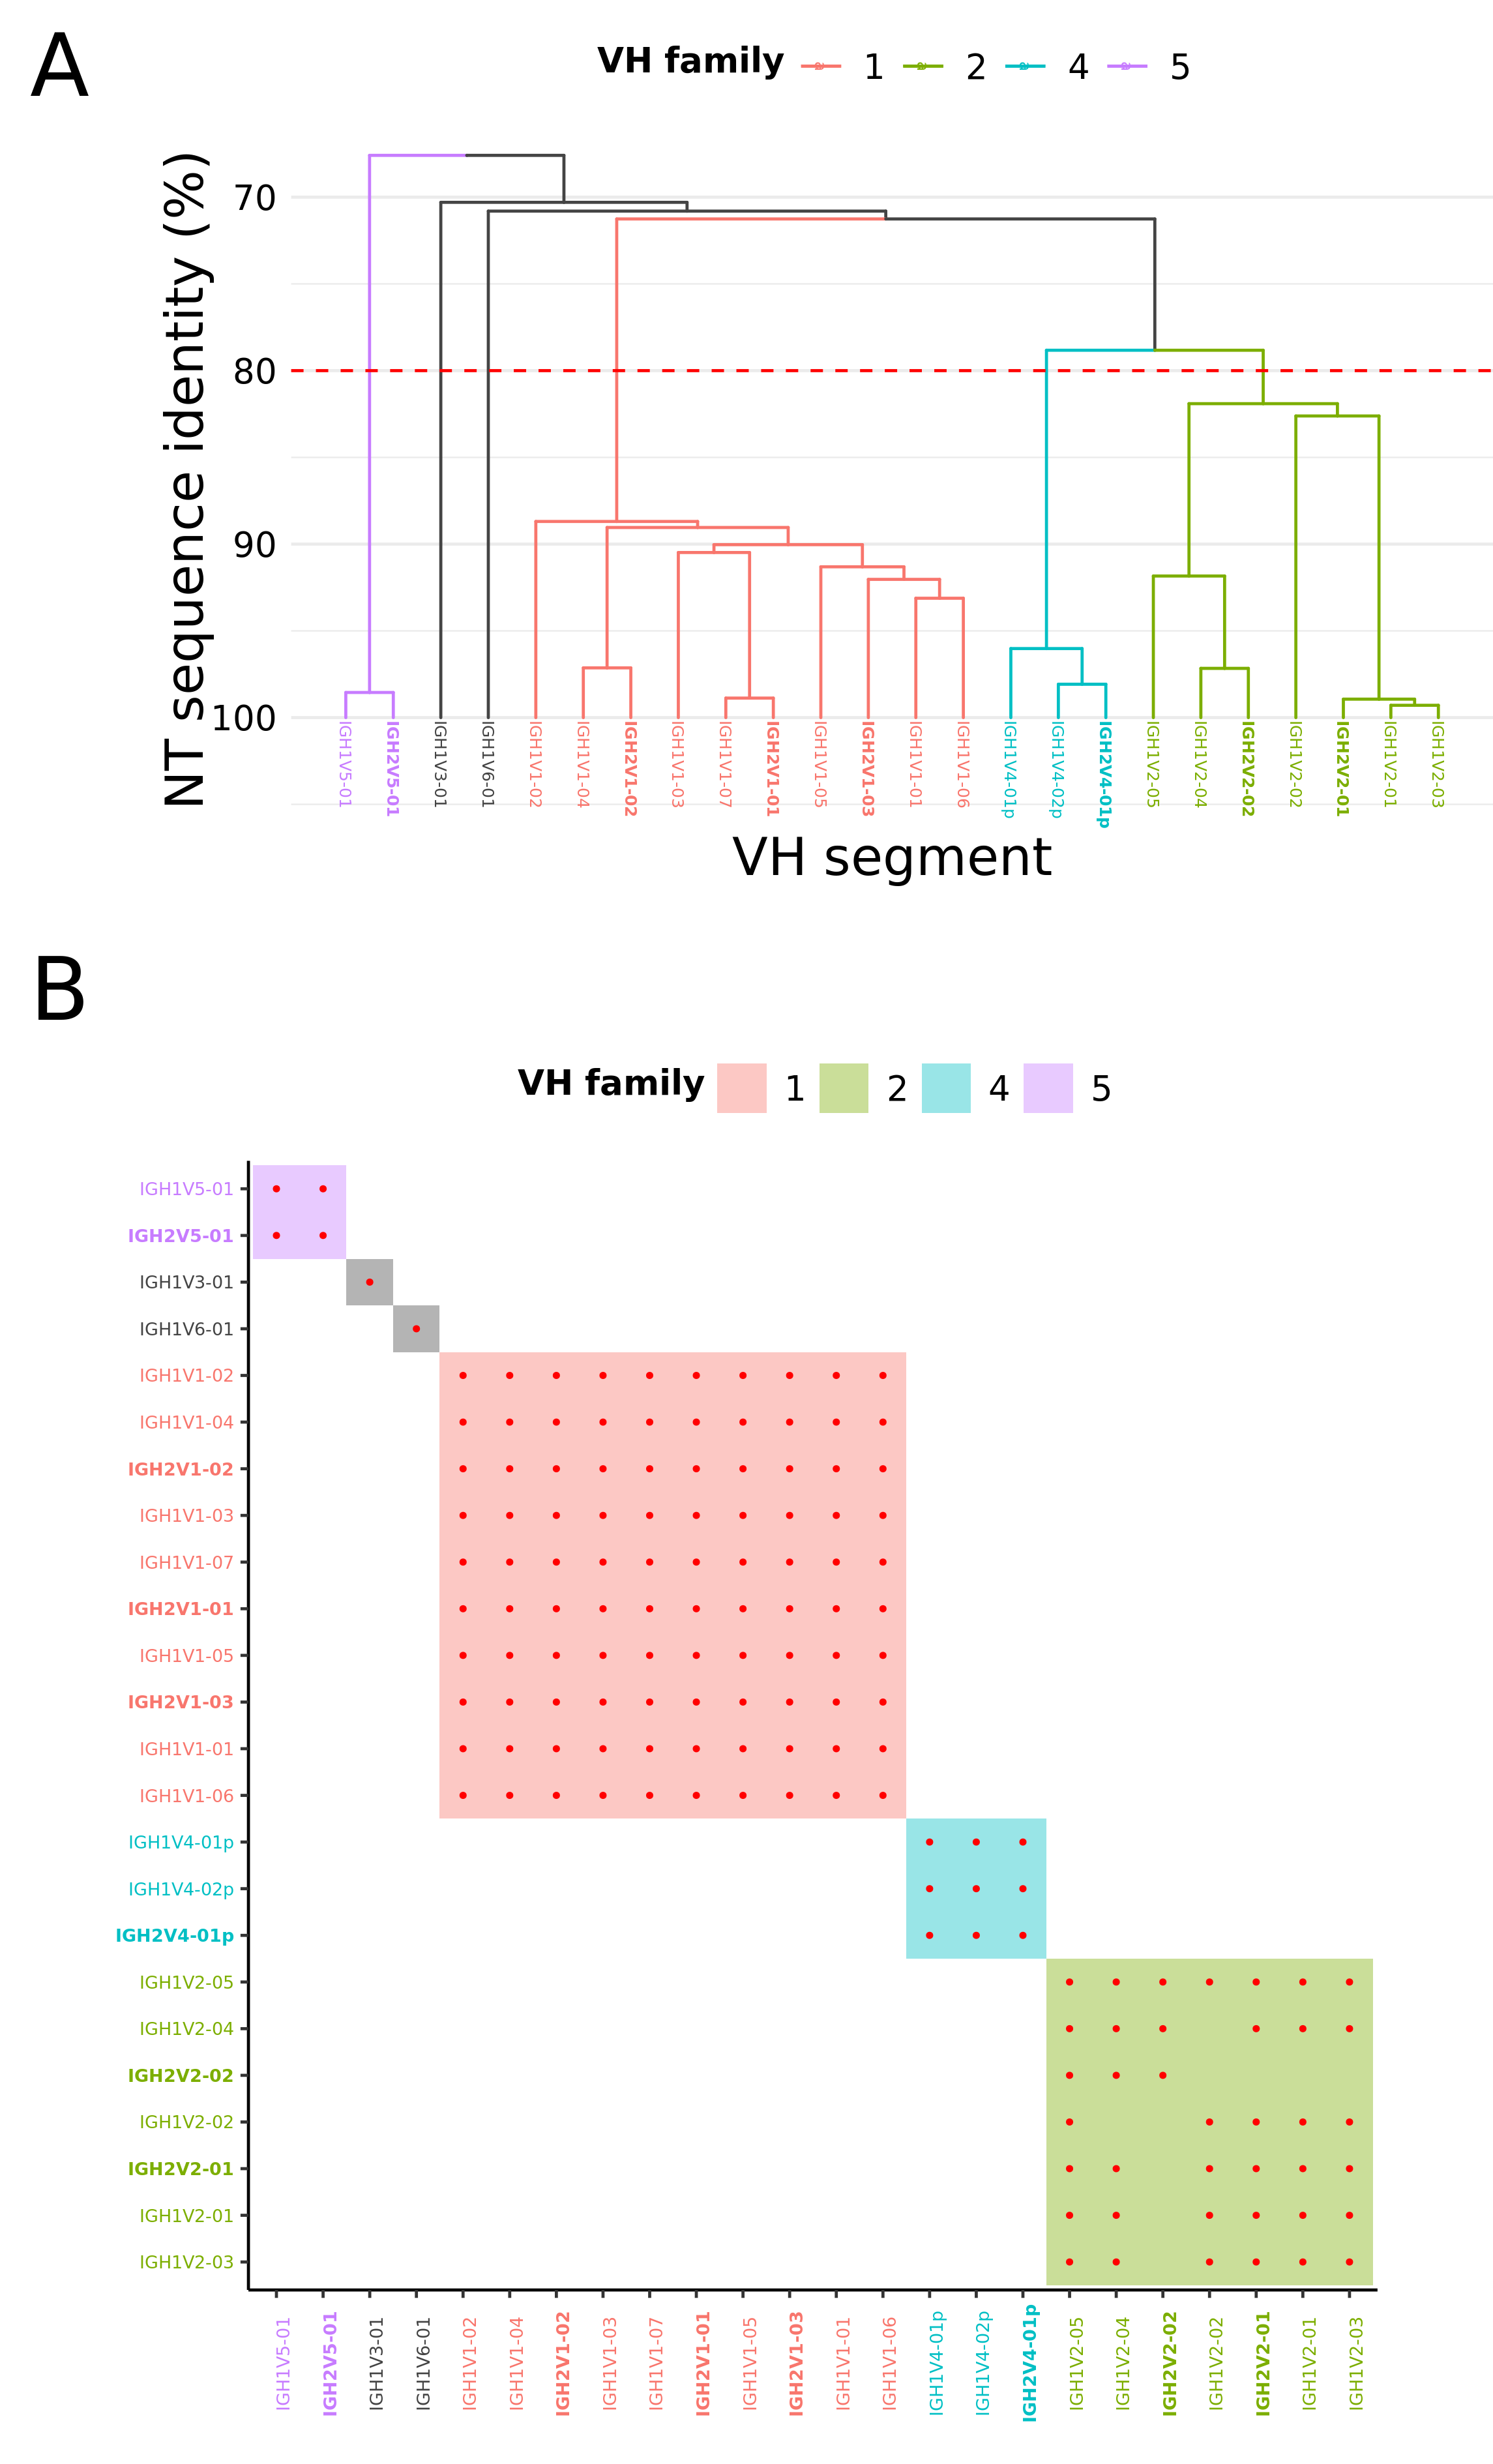
\includegraphics[width=0.8\textwidth]{_Figures/png/nfu-vh-families.png}
	\Caption{\vh families in the \Nfu \igh{} locus}{(A) Dendrogram of sequence similarity of \vh segments in the \Nfu \igh{} locus, arranged by single-linkage clustering on nucleotide sequence identity. The red line indicates the 80\,\% cutoff point for family assignment. (B) Heatmap of family relationships among \Nfu \vh segments, with shaded squares indicating families and red dots indicating pairwise nucleotide sequence identity of at least 80\,\%. In both subfigures, \vh families containing multiple segments are uniquely coloured, single-segment families are in grey, and segments from the \igh{2} sublocus are displayed in boldface.}
	\label{fig:nfu-vh-families}
	\end{figure}

\begin{figure}
\centering
	\centering
	\begin{subfigure}{0em}
	\phantomsubcaption{}
    \label{fig:nfu-dj-alignment-a}
    \end{subfigure}
    \begin{subfigure}{0em}
    \phantomsubcaption{}
    \label{fig:nfu-dj-alignment-b}
    \end{subfigure}
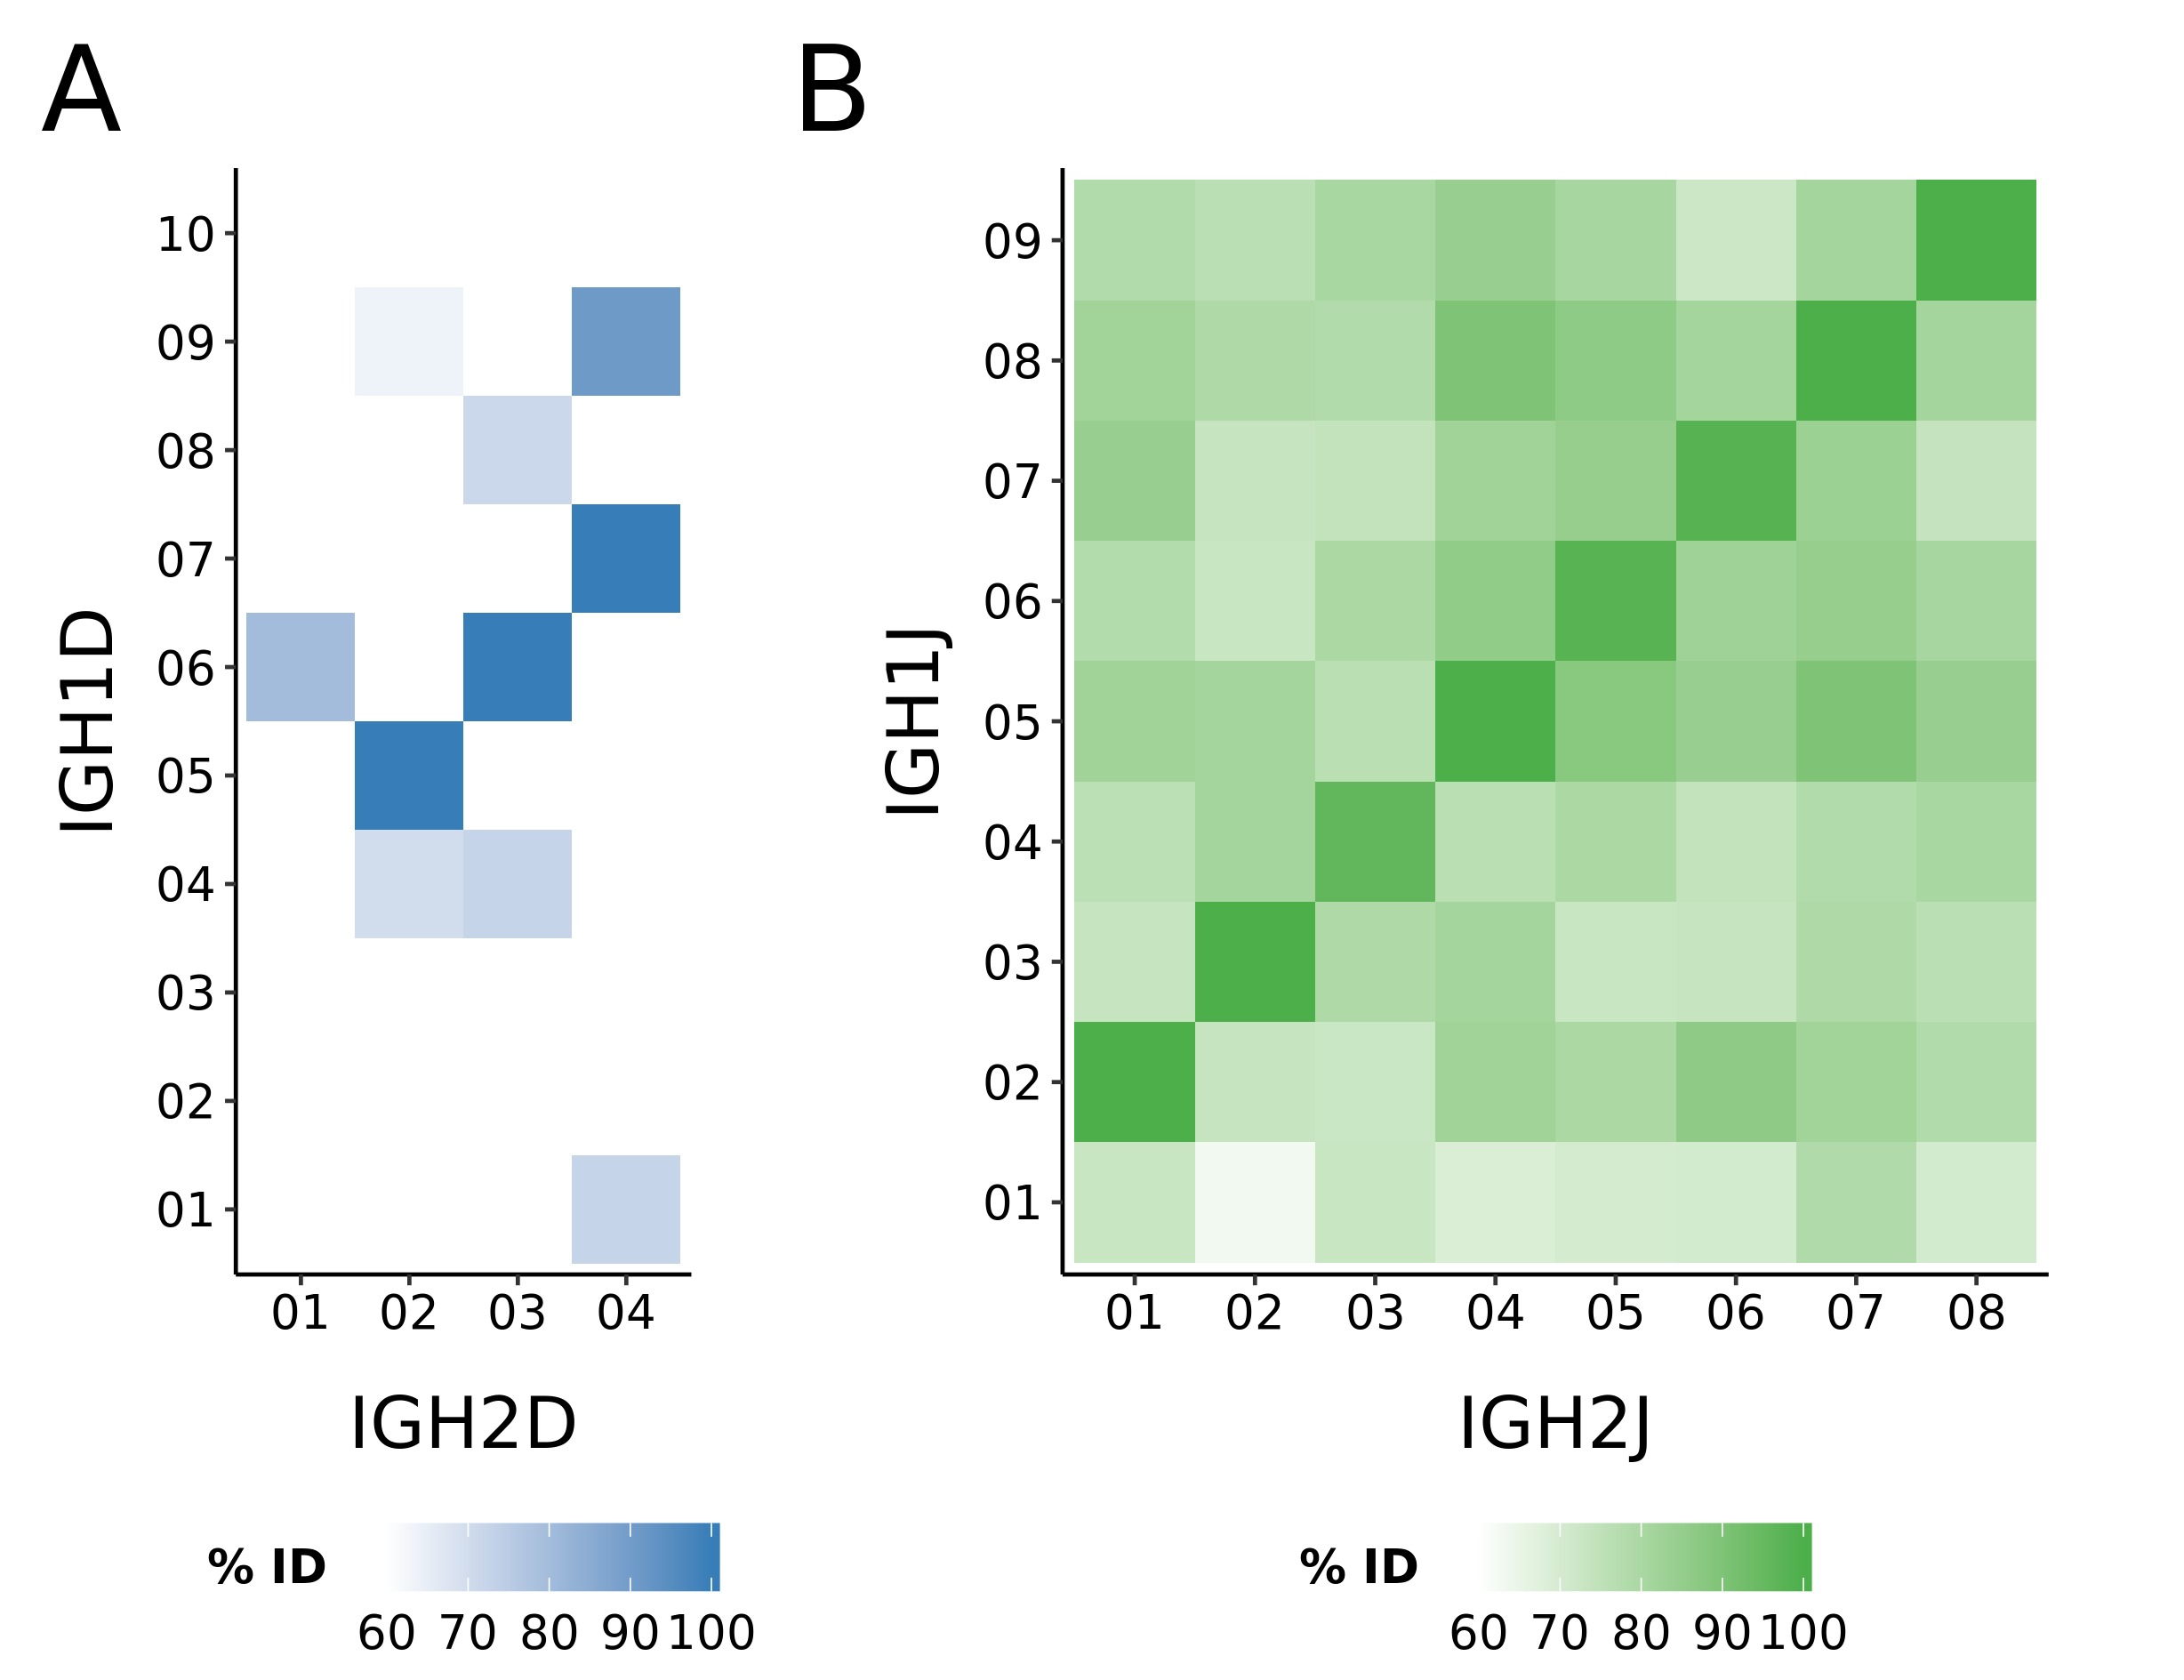
\includegraphics[width=0.6\textwidth]{_Figures/png/nfu-dj-aln}
\Caption{Cross-sublocus sequence similarity of \dh and \jh gene segments in \Nfu \igh{}}{Heatmap of percentage nucleotide sequence identities of Needleman-Wunsch global alignments between (A) \dh and (B) \jh gene segments in \igh{1} vs \igh{2}, revealing syntenic runs of highly similar sequences across both subloci.}
\label{fig:nfu-dj-alignment}
\end{figure}	
	
	\begin{figure}
	\centering
	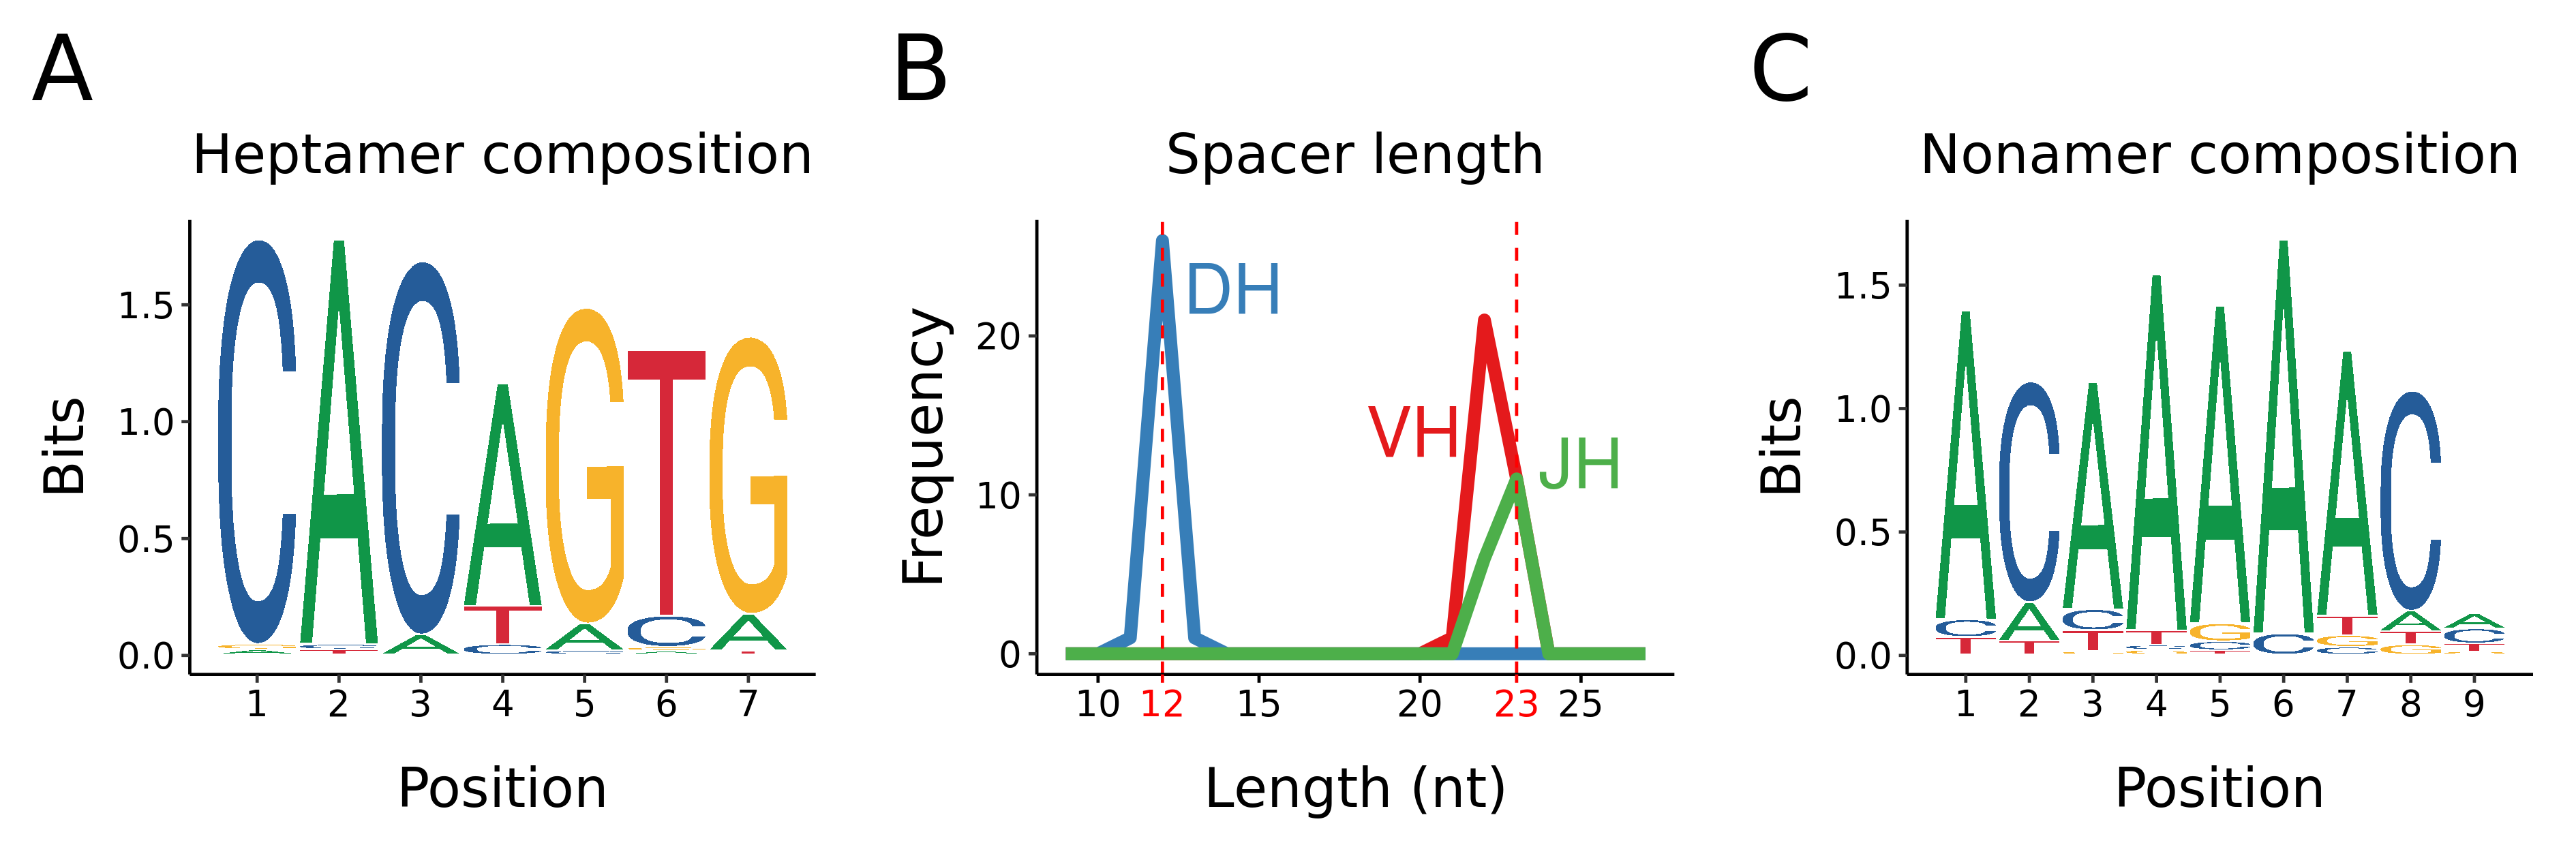
\includegraphics[width=\textwidth]{_Figures/png/nfu-rss-seqlogo-all}
	\Caption{Recombination signal sequences in \Nfu \igh{}}{(A) Sequence composition of conserved heptamer sequences across all \Nfu heavy-chain RSSs; (B) length distribution of unconserved spacer sequences in \Nfu heavy-chain RSSs; (C) sequence composition of conserved heptamer sequences across all \Nfu heavy-chain RSSs.}
	\label{fig:nfu-rss-seqlogo-all}
	\end{figure}
	
\FloatBarrier
\clearpage

\section{The \igh{} locus in \xma}
\label{sec:xma-locus}
	
	The turquoise-killifish \igh{} locus shares many features with other characterised teleost loci, including a modified tandem-translocon configuration with intact \vh, \dh, \jh and constant regions (\Cref{fig:nfu-locus-map-b}), a four-exon secreted configuration of \igh{M} (\Cref{fig:nfu-locus-sashimi-a}), an expanded \igh{D} constant region with tandem \cd{}-exon block repeats (\Cref{fig:nfu-locus-sashimi-b,fig:nfu-locus-map-b},), a conserved RSS structure (\Cref{fig:nfu-rss-seqlogo-all}), and a chimeric \cm{1} in \igh{D} (\Cref{fig:nfu-locus-sashimi-b}). However, it also exhibits many ideosyncratic features that differ from those observed in most characterised teleost loci, including an unusually small number of \vh segments (\Cref{fig:nfu-vh-families} and \Cref{tab:teleost-vh-counts}), a four-exon \cm{1}-\cm{2}-TM1-TM2 configuration of transmembrane \igh{M} (\Cref{fig:nfu-locus-sashimi-a}), an inverted sublocus present in antisense (\Cref{fig:nfu-locus-map-b}), and a complete absence of \igh{Z}.
	
Many of these peculiarities, including the unusual \igh{M-TM} splicing pattern, inverted sublocus, and lack of \igh{Z}, are shared with the \igh{} locus of medaka (\textit{Oryzias latipes}), which is the closest relative of \textit{Nothobranchius furzeri} to have its immunoglobulin heavy chain locus characterised prior to this study \parencite{magadan2011medaka}. Given the close relationship between the two species, the shared unusual features of their \igh{} loci suggested a common origin of these traits  in the common ancestor of both species. If this hypothesis were correct, one would expect \igh{Z} to also be absent in any other descendents of this common ancestor, including other cyprinodontiform species.

To investigate this hypothesis further, I performed a complete characterisation of the \igh{} locus in the platyfish \textit{Xiphophorus maculatus}, another cyprinodontiform species that has seen widespread use as a model organism \parencite{schartl2013platyfish}. Surprisingly, the \Xma locus possessed none of the unusual features shared between the turquoise-killifish and medaka loci, strongly suggesting independent loss of \igh{Z} in \Nfu and medaka and implying a high level of volatility in \igh{} locus structure in this group of teleost fishes.

\subsection{Overall structure}
\label{sec:xma-locus-structure}
	
As was the case with the \Nfu \igh{} locus, I identified candidate genome scaffolds from the most recent \xma genome assembly (Genbank accession GCA\_002775205.2) by aligning them to \igh{} gene segments from zebrafish, stickleback and medaka, supplemented in this case with segments from the newly-characterised \Nfu locus itself. In contrast to the more fragmented results in \Nfu, this process identified a single sequence region on one chromosome of the \Xma locus, which I extracted and characterised as described for the assembled \Nfu locus (\Cref{sec:nfu-locus}) without the need for further sequencing or assembly.

The \Xma \igh{} locus so identified occupies roughly \kb{293} on chromosome 16 (scaffold NC\_036458.1; \Cref{fig:xma-locus-map-a}). Unlike in turquoise killifish and medaka, all identified gene segments share a common orientation; no evidence of a second sublocus in antisense could be identified. In stark contrast with both turquoise killifish and medaka, the single ``sublocus'' comprising \Xma \igh{} contains not one but two \igh{Z} constant regions, along with a hugely extended V-region extending over almost \kb{250} and containing more than 120 \vh-segments (\Cref{fig:xma-locus-map-b}). This enormous \vh-diversity exceeds that of almost all previously-characterised teleost \igh{} loci (\Cref{sec:intro_teleost_loci}), while the presence of multiple \igh{Z} constant regions without intervening \igh{M} or \igh{D} is also highly unusual \parencite{fillatreau2013astonishing}. 

Even cursory examination of the \Xma \igh{} locus is therefore sufficient to reveal a unique and highly interesting structure with many unexpected differences from both turquoise killifish and medaka (\Cref{fig:species-tree-small}, columns 1-5). In particular, since \Xma is more closely related to \Nfu than either is to medaka, the presence of \igh{Z} in the former strongly suggests at least two independent loss events in the lineage containing turquoise killifish and medaka, indicating an unexpected level of volatility in the evolution of this important isotype.
 
	\begin{figure}
	\centering
	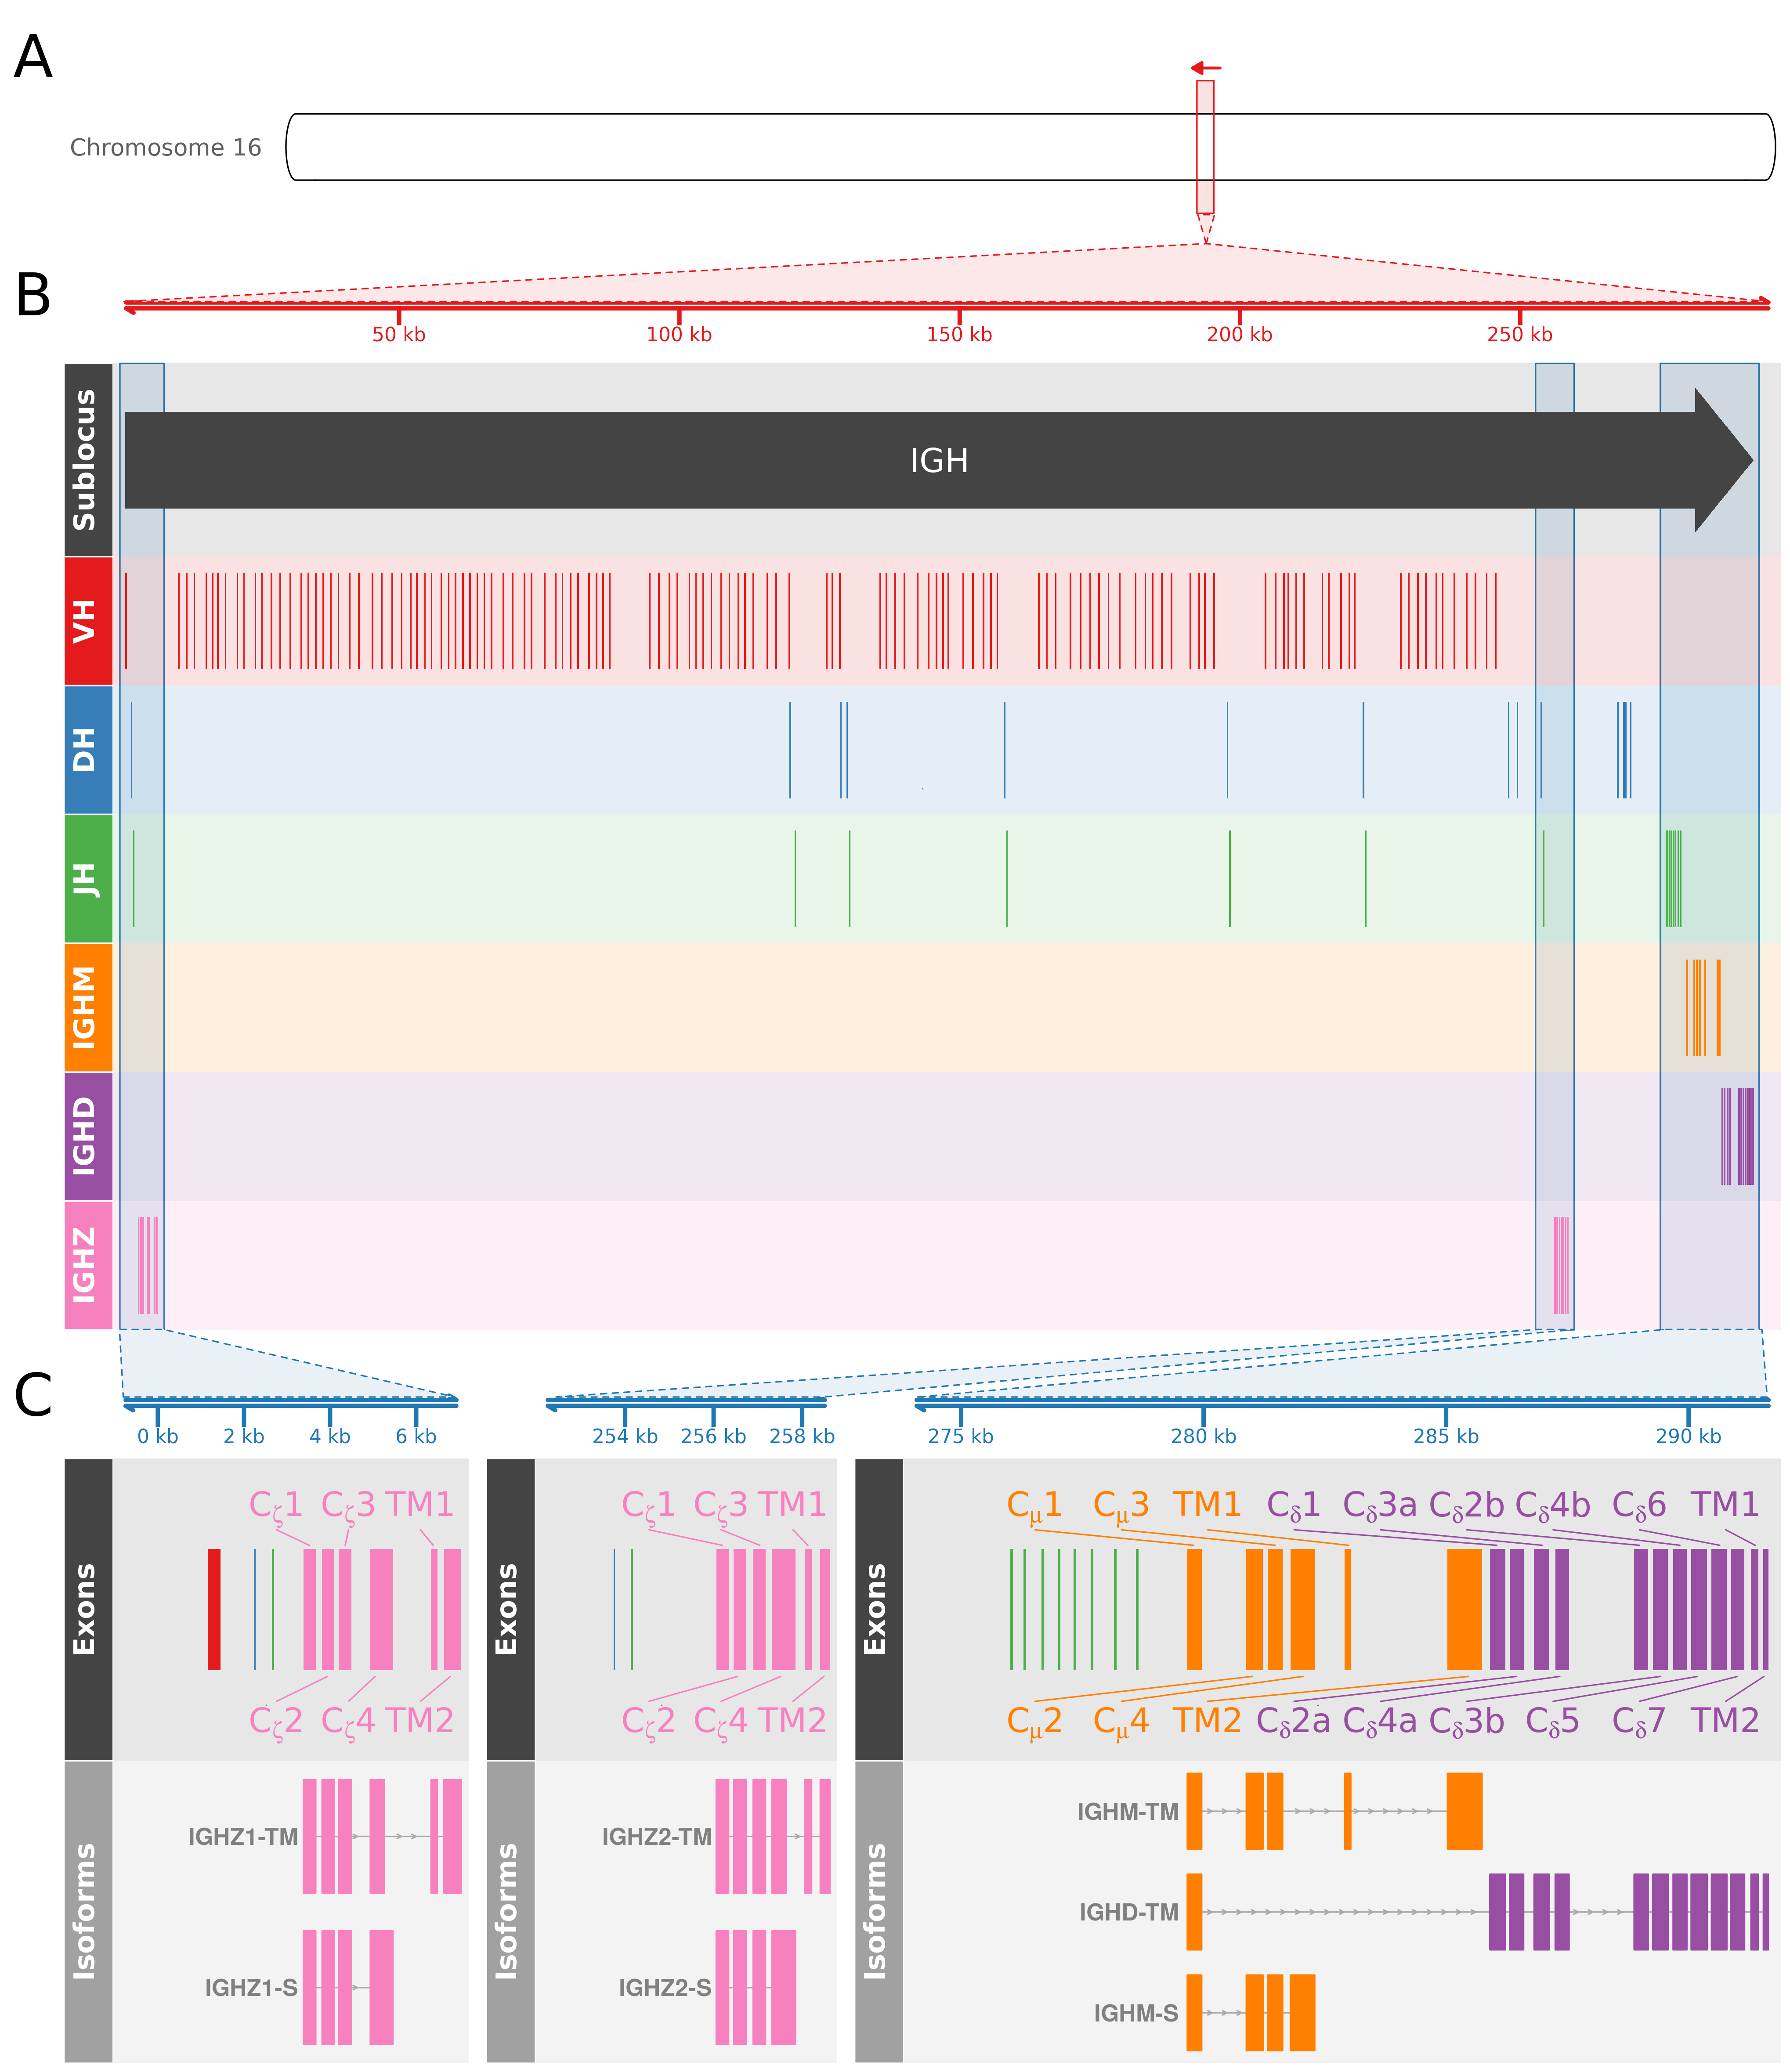
\includegraphics[width=\textwidth]{_Figures/png/xma-new-locus-map}
	\Caption{The immunoglobulin heavy chain (\igh{}) locus in \xma}{(A) Position of the \igh{} locus on chromosome (group) 16 of the \Xma genome. (B) Arrangement of \vh, \dh, \jh and constant-region gene segments on the \Xma \igh{} locus. (C) Detailed map of the \igh{Z1}, \igh{Z2} and \igh{M/D} constant regions, indicating the position and identity of the constant-region exons and the exon composition of expressed \igh{} isoforms in \Xma. Note change of orientation between subfigures (A) and (B-C).}
	\begin{subfigure}{0em}
        \phantomsubcaption{}
        \label{fig:xma-locus-map-a}
    \end{subfigure}
    \begin{subfigure}{0em}
        \phantomsubcaption{}
        \label{fig:xma-locus-map-b}
    \end{subfigure}
    \begin{subfigure}{0em}
        \phantomsubcaption{}
        \label{fig:xma-locus-map-c}
    \end{subfigure}
	\label{fig:xma-locus-map}
\end{figure}

\begin{figure}
\centering
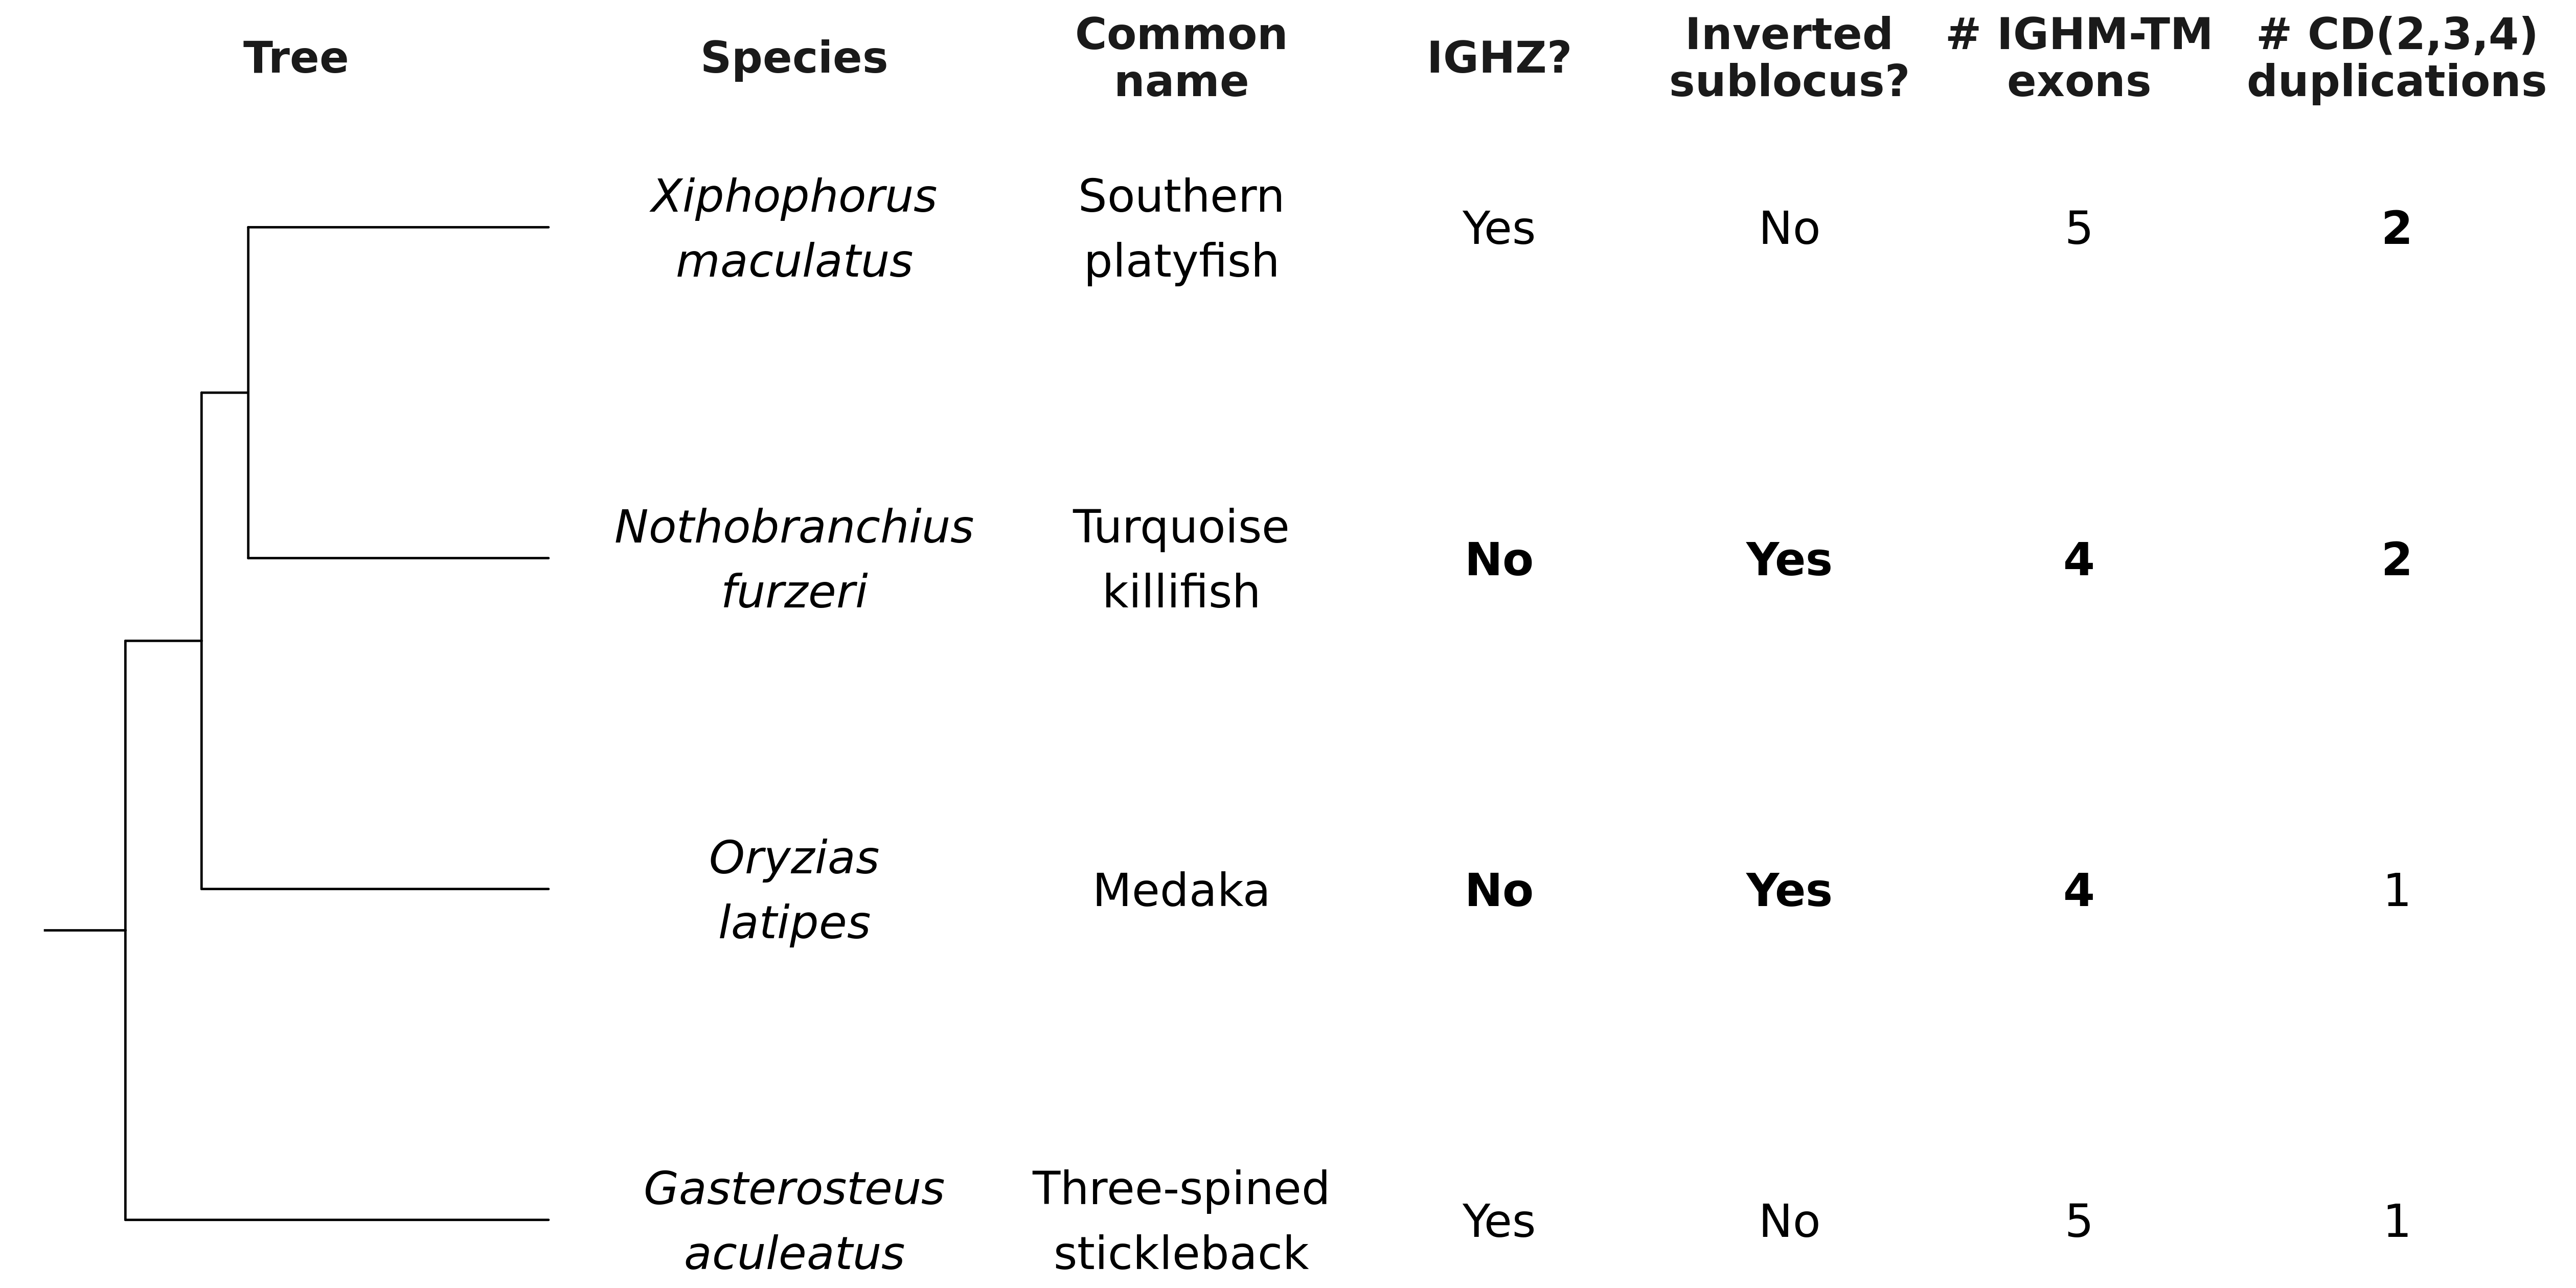
\includegraphics[width=\textwidth]{_Figures/png/species-tree-small}
\vspace{0.5em}
\Caption{Important \igh{} phenotypes in turquoise killifish, southern platyfish, and medaka}{Cladogram of the evolutionary relationship between southern platyfish (\xma), turquoise killifish (\nfu) and medaka (\species{Oryzias}{latipes}), with three-spined stickleback (\species{Gasterosteus}{aculeatus}) as an outgroup. The state of various \igh{} phenotypes of interest are annotated to the right of the tree; states deviating from the expected teleost configuration are in bold.}
\label{fig:species-tree-small}
\end{figure}
	
\subsection{Constant regions}
\label{sec:xma-locus-constant}
	
As discussed briefly in \Cref{sec:xma-locus-structure}, the \Xma \igh{} locus contains two distinct \igh{Z} constant regions: one in the usual position immediately preceding the \igh{M}-associated D- and J-regions, the other, unexpectedly, at the far 5'-extremity of the locus (\Cref{fig:xma-locus-map-b}). Both \igh{Z} constant regions occupy the expected configuration, with four \cz{} exons, two transmembrane exons, and a secretory tail (\Cref{fig:xma-locus-map-c}, \Cref{tab:xma-ch-coords}). However, in contrast to the duplicate constant regions in \Nfu, the two \igh{Z} constant regions in \Xma are quite distinct from each other in sequence, with an average of only \pc{64} nucleotide and \pc{48} amino-acid sequence identity between corresponding \cz{} exons (\Cref{fig:xma-cz-aln}, \Cref{tab:xma-cz-aln}). This unexpectedly high level of sequence divergence suggests a relatively ancient duplication event, and raises the possibility that the lineage giving rise to \Nfu may have lost not one, but two distinct \igh{Z} constant regions.
	
\begin{table}
	\centering
	\Caption{Sequence similarity between \igh{Z} constant-regions in \Xma}{Percentage sequence identities of pairwise Needleman-Wunsch global alignments between nucleotide (NT) or amino-acid (AA) sequences of corresponding \cz{} exons from the two \igh{Z} constant regions of \Xma \igh{}.}
	% latex table generated in R 3.5.2 by xtable 1.8-3 package
% Tue Jan  8 14:15:22 2019
\begin{tabular}{llrr}
  \toprule Isotype & Exon & NT & AA \\ 
  \midrule Z & 1 & 59.14 & 44.57 \\ 
  Z & 2 & 63.93 & 53.41 \\ 
  Z & 3 & 66.19 & 43.48 \\ 
  Z & 4 & 65.15 & 50.49 \\ 
   \bottomrule \end{tabular}

	\label{tab:xma-cz-aln}
\end{table}

While the state of \igh{Z} constant regions differs markedly between \Xma and \Nfu, the configurations of the \igh{M} and \igh{D} constant regions of the two species are quite similar, with a {\cm{1}-\cm{2}-\cm{3}-\cm{4}-TM1-TM2} configuration for \igh{M} and a {\cd{1}-(\cd{2}-\cd{3}-\cd{4})$_2$-\cd{5}-\cd{6}-\cd{7}-TM1-TM2} configuration for \igh{D} (\Cref{fig:xma-locus-map-b,fig:xma-locus-map-c}, \Cref{tab:xma-ch-coords}). In the \Xma locus, these constant regions and \igh{Z2} adopt the standard configuration seen in comparatively simple teleost \igh{} loci like those of zebrafish and fugu, with a {\vh-\dh-\jh-\textbf{CZ}-\dh-\jh-\textbf{CM}-\textbf{CD}} arrangement that allows the choice between \igh{Z} and \igh{M/D} usage to be made via the choice of \dh segment during VDJ-recombination. However, whether such a mechanism is also responsible for the choice between these constant regions and \igh{Z1}, which lies more than \kb{200} away and upstream of the great majority of \vh segments in the locus (\Cref{sec:xma-locus-variable}) is questionable.

In order to investigate the expressed isoforms present in \Xma, I aligned published RNA-sequencing reads from various platyfish tissues (BioProject accession PRJNA420092, all libraries, \Cref{tab:rnaseq-sources}) to the \igh{Z} and \igh{M/D} constant regions with \program{STAR}. The results indicate the expected six-exon transmembrane configuration in both \igh{Z1} and \igh{Z2}, as well as a secretory form of \igh{Z1} comprising \cz{1} to \cz{4} plus a \bp{23} secretory tail formed by a transcriptional run-on event from \cz{4} (\Cref{fig:xma-locus-sashimi-z1,fig:xma-locus-sashimi-z2}). However, while an in-frame secretory tail of similar length (\bp{20}) can be found in \igh{Z2}, it does not appear to be expressed in the read sets analysed here, suggesting that \igh{Z2} may only be expressed in transmembrane form in the individuals sampled (\Cref{fig:xma-locus-sashimi-z2}).

Meanwhile, the results for \igh{D} (\Cref{fig:xma-locus-sashimi-d}) indicate a similar configuration to that observed in turquoise killifish, with a chimeric \cm{1} followed by 10 \cd{} exons and two transmembrane exons; as in \Nfu, neither a dedicated \igh{D} secretory exon nor a post-\cd{7} secretory tail was identified, suggesting that \igh{D} may be produced solely in transmembrane form in \Xma. Secretory \igh{M} (\igh{M-S}) was also found to occupy the same four-exon configuration seen in turquoise killifish and elsewhere. However, the configuration observed for transmembrane \igh{M} (\igh{M-TM}) did not correspond to the four-exon structure shared between turquoise killifish and medaka (\Cref{fig:xma-locus-sashimi-m,fig:nfu-locus-sashimi-a}); rather, \igh{M-TM} in \Xma occupies the five-exon configuration seen in most characterised teleosts (\Cref{fig:teleost-igm-exons-d}). This surprising difference indicates that two different splice configurations of \igh{M-TM} persist in the cyprinodontiform lineage, and raises the question of what, if any, functional difference arises from the presence or absence of \cm{3} in transmembrane \igh{M} in different species. However, it remains unclear whether this pattern of exon usage (\Cref{fig:species-tree-small}) is the result of independent changes in medaka and turquoise killifish or of a reversion in \Xma to the primitive teleost configuration.
	
\begin{figure}
	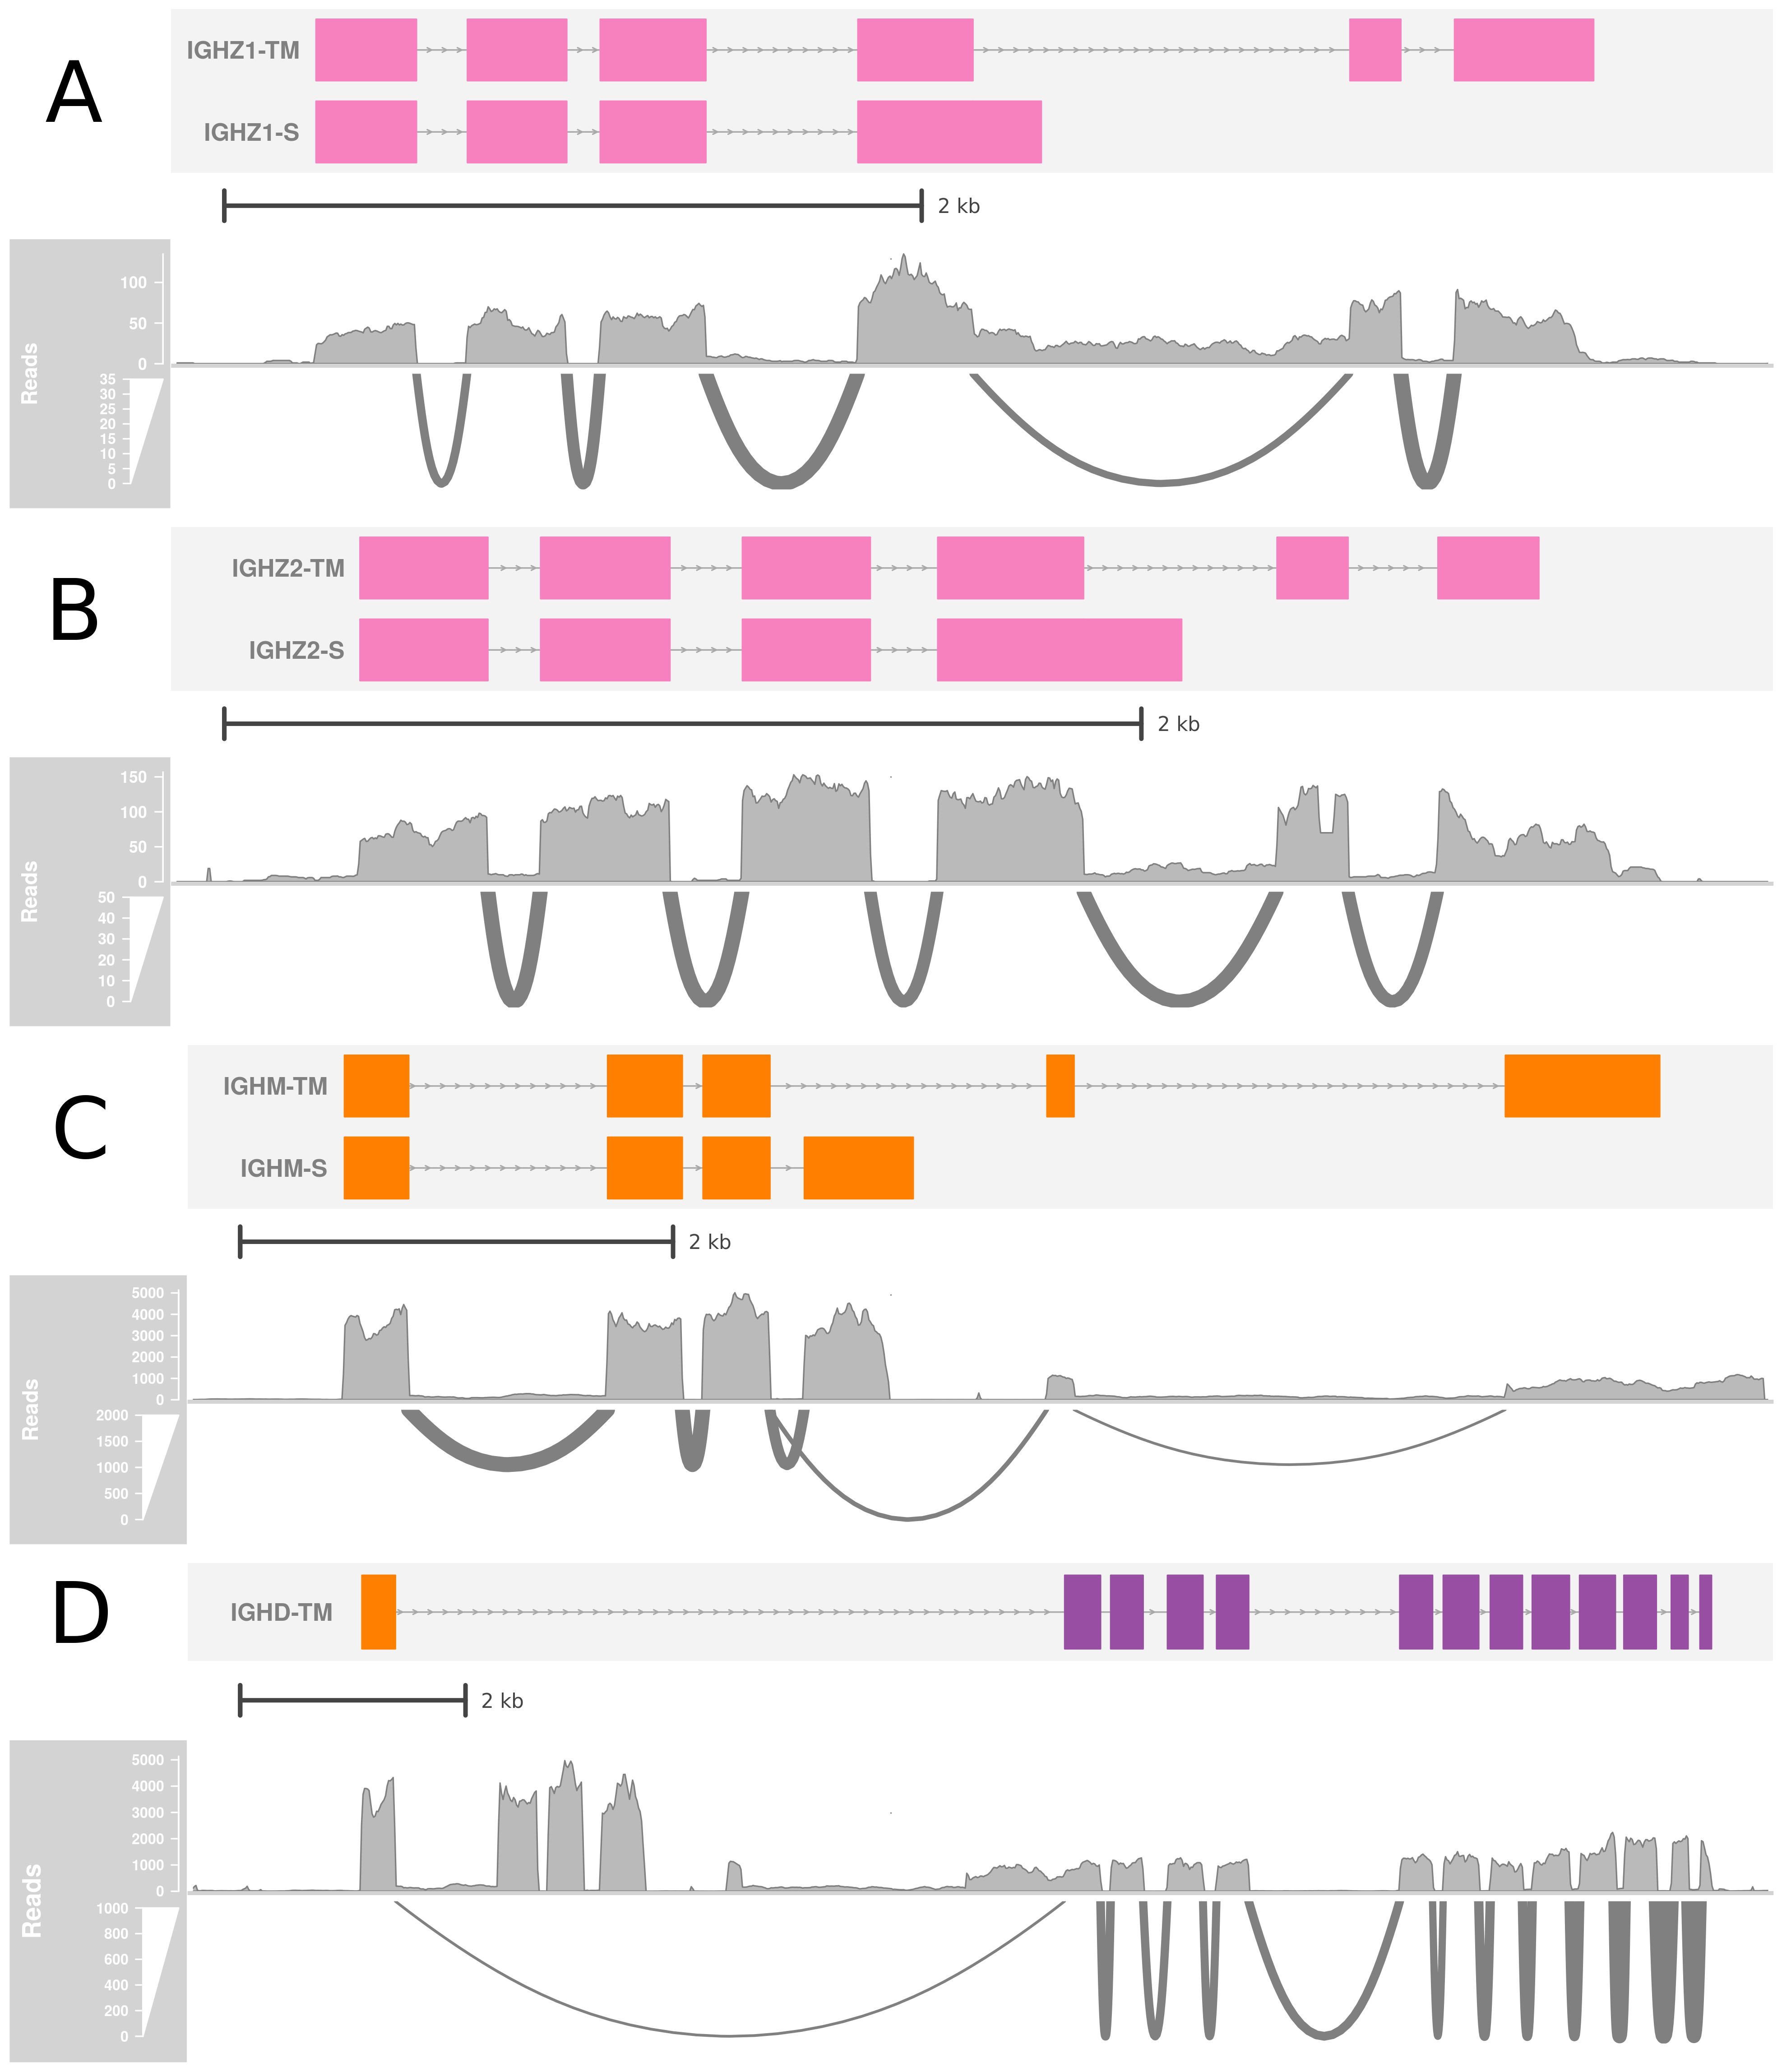
\includegraphics[width=\textwidth]{_Figures/png/xma-new-locus-sashimi}
	    \begin{subfigure}{0em}
        \phantomsubcaption{}
        \label{fig:xma-locus-sashimi-z1}
    \end{subfigure}
    \begin{subfigure}{0em}
        \phantomsubcaption{}
        \label{fig:xma-locus-sashimi-z2}
    \end{subfigure}
	\begin{subfigure}{0em}
        \phantomsubcaption{}
        \label{fig:xma-locus-sashimi-m}
    \end{subfigure}
    \begin{subfigure}{0em}
        \phantomsubcaption{}
        \label{fig:xma-locus-sashimi-d}
    \end{subfigure}
	\Caption{Constant-region isoforms in \Xma}{Coverage and Sashimi plots \parencite{katz2013sashimi} of STAR-aligned RNA-seq reads from \Xma samples, demonstrating the splicing behaviour of \igh{} constant-region isoforms and showing the read coverage of each exon and splice junction. (A) \igh{Z1} exon splicing, showing alternative use of the \cz{4}/TM1 splice junction and the post-\cz{4} secretory tail; (B) \igh{Z2} exon splicing, showing the apparent lack of expression of the \igh{Z2} secretory isoform; (C) \igh{M} exon splicing, showing alternative splicing patterns of \igh{M-TM} and \igh{M-S}; (D) \igh{D} exon splicing, showing chimeric splicing of \cm{1} to \cd{1}.}
	\label{fig:xma-locus-sashimi}
	\end{figure}

	
\subsection{Variable regions}
\label{sec:xma-locus-variable}

In total, I identified 125 \vh segments, 14 \dh segments and 15 \jh segments in the \Xma \igh{} locus (\Cref{fig:xma-locus-map-b}). Of these, exactly one \vh (\igh{V01-01}), \dh (\igh{DZ01}) and \jh (\igh{JZ01}) lie upstream of the \igh{Z1} constant region, indicating that the variable-region sequence diversity available to this isotype is limited to a single VDJ combination. In contrast, the variable region between the end of \igh{Z1} and the start of \igh{Z2} is highly expanded, with 124 tightly-clustered \vh segments -- more than five times the total number seen in \Nfu, and more than seven times the number in the largest \Nfu sublocus. Of these 124 \vh segments, 106 (\pc{86}) are apparently functional, with the remainder pseudogenised by a variety of frameshift mutations, nonsense mutations, or truncation events (\Cref{tab:xma-vh-coords-1,tab:xma-vh-coords-2,tab:xma-vh-coords-3,tab:xma-vh-coords-4,tab:xma-vh-coords-5}); it remains to be seen whether \igh{V01-01} is also capable of recombining with \dh segments downstream of the \igh{Z1} constant region, and so constitutes part of the range of VDJ combinations available to the other constant regions. The \vh sequences in the \Xma locus are much more tightly packed than in the \Nfu locus, consistent with a lower overall prevalence of repetitive regions (21\,\%) in the \Xma genome \parencite{yuan2018repeats}.
	
In total, the \vh regions in \Xma \igh{} fall into 23 families, of which eight contain multiple segments (\Cref{fig:xma-vh-families-tree,fig:xma-vh-families-map}); strikingly, the single \vh segment serving \igh{Z} (\igh{V01-01}) represents a separate family which is distinct from any other segment in the locus. To further investigate the evolutionary history of these families, I aligned the \vh segments from both the \Xma and \Nfu \igh{} loci together with \program{PRANK}, and used the resulting alignment to construct a phylogenetic tree with \program{RAxML} \parencite{stamatakis2014raxml8,stamatakis2005raxml3,stamatakis2006raxml6}; the resulting tree (\Cref{fig:nfu-xma-vh-tree-nt}) revealed a clear interrelationship between the largest families in both loci (\Xma V02 and \Nfu V1), with a similar relationship observed for the second-largest families (\Xma V03 and \Nfu V2). 
In accordance with the close sequence relationship noted in \Cref{sec:nfu-locus-variable}, \Nfu V4 falls comfortably within the V03/V2 subtree, supporting its status as a pseudogenised subfamily of \Nfu V2.
		
In addition to its highly expanded \vh region, the variable region of the \Xma locus is unusual in the arrangement of its \dh and \jh segments (\Cref{tab:xma-dh-coords-seg,tab:xma-jh-coords-seg}): in addition to the relatively densely-packed blocks of four \dh and eight \jh segments between \igh{Z2} and \igh{M}, and the smaller groups of three \dh segments and one \jh segment between the last \vh segment and \igh{Z2}, small numbers of \dh and \jh segments are interspersed between blocks of \vh segments in the extended V-region between \igh{Z1} and \igh{Z2} (\Cref{fig:xma-locus-map-b}). Many of these segments are arranged such that groups of one or two \dh segments are closely associated with a single \jh segment, raising the possibility of a more cluster-like behaviour in which each VDJ block acts as a distinct recombination unit. However, the presence of larger D- and J-regions more closely upstream of the constant regions suggests a more conventional translocon behaviour; it remains to be seen which of these traditional models of antigen-receptor structure more closely matches the \textit{in vivo} recombination behaviour of this locus.
		
Finally, as is the case with \Nfu, the recombination signal sequences (RSSs) in \Xma \igh{} correspond closely to the standard expectations across the vertebrates, with the expected heptamer and nonamer consensus sequences and spacer length distributions (\Cref{fig:xma-rss-seqlogo-all,fig:xma-rss-seqlogo-sep}, 97.6\,\% of RSS spacers within \bp{1} of the expected conserved length).	

	\begin{figure}
		\begin{subfigure}{0em}
        \phantomsubcaption{}
        \label{fig:xma-rss-seqlogo-all-heptamer}
    \end{subfigure}
    \begin{subfigure}{0em}
        \phantomsubcaption{}
        \label{fig:xma-rss-seqlogo-all-spacer}
    \end{subfigure}
    \begin{subfigure}{0em}
        \phantomsubcaption{}
        \label{fig:xma-rss-seqlogo-all-nonamer}
    \end{subfigure}
	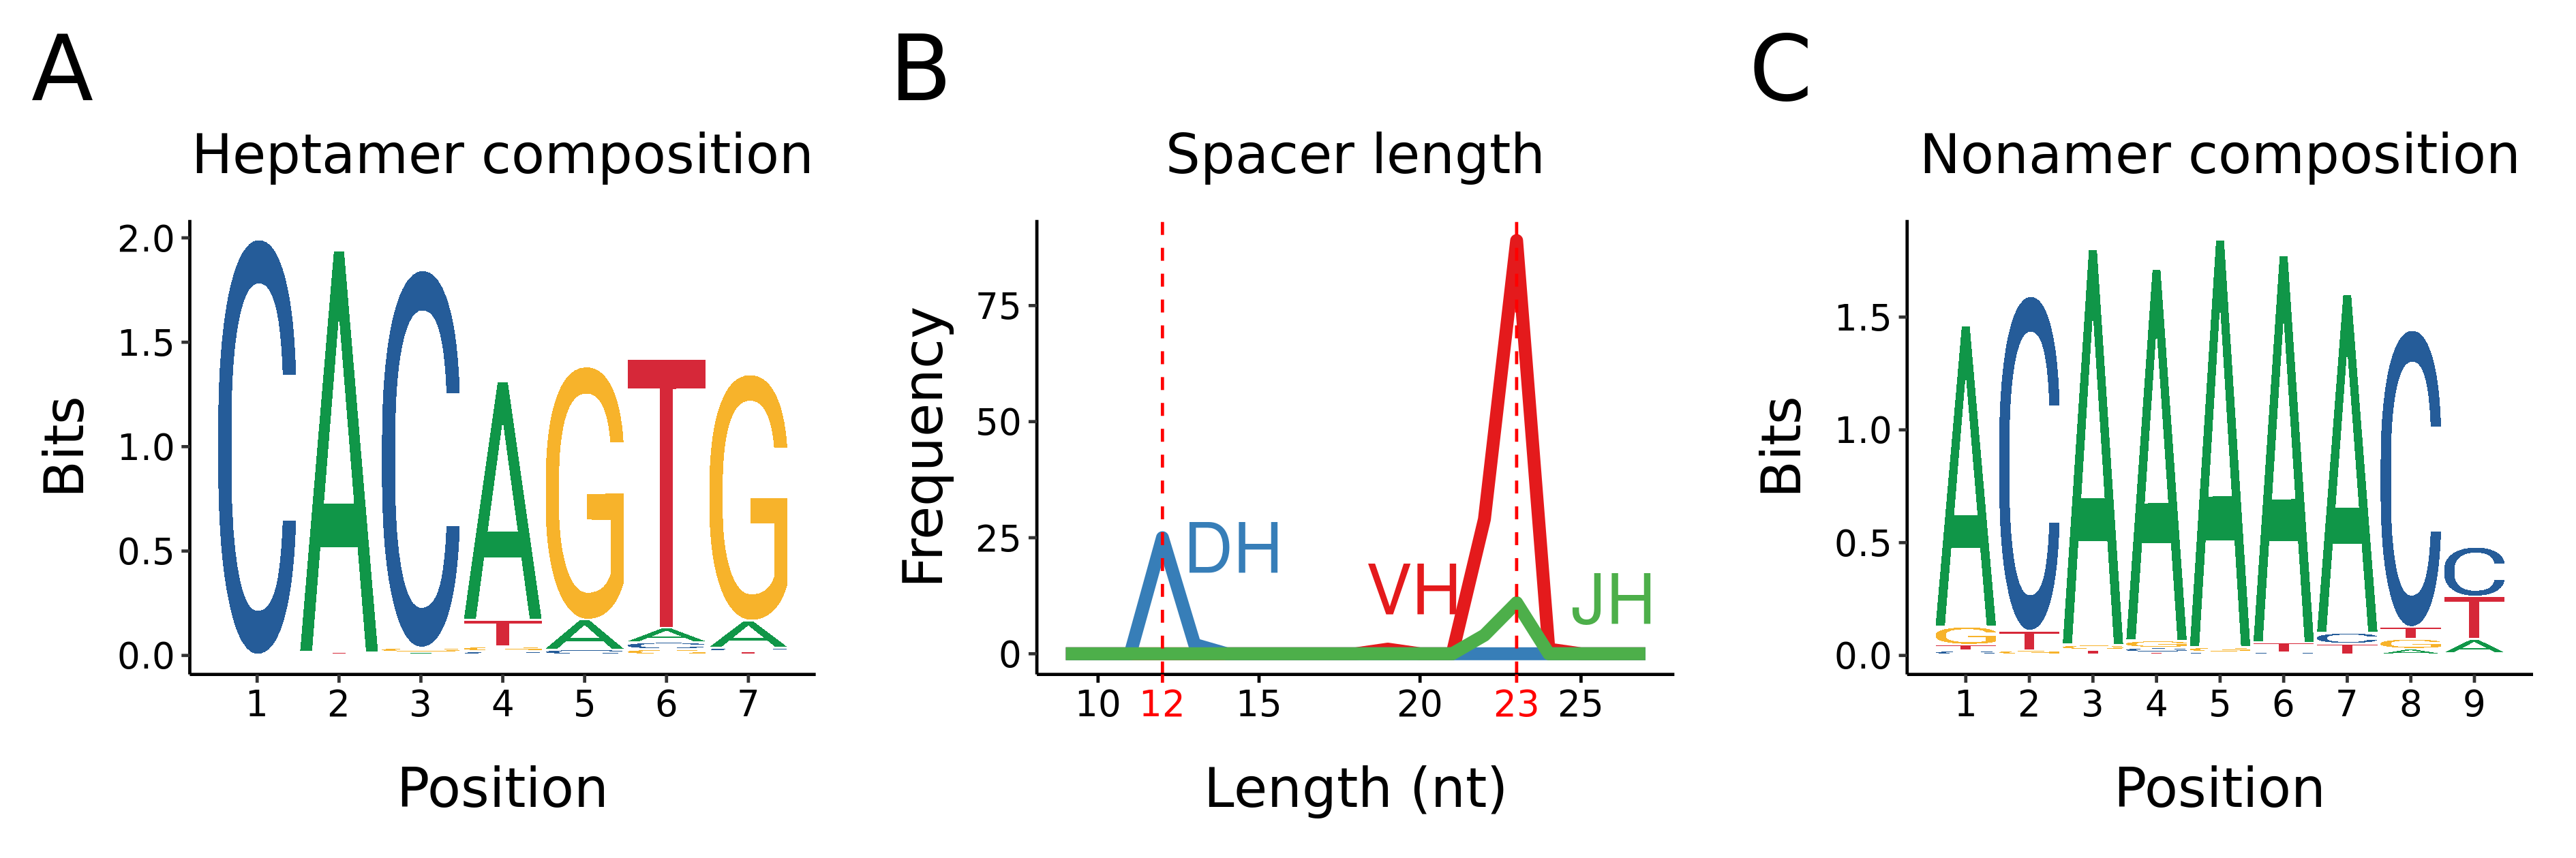
\includegraphics[width=\textwidth]{_Figures/png/xma-new-rss-seqlogo-all}
	\Caption{Recombination signal sequences in the \Xma \igh{} locus}{(A) Sequence composition of conserved heptamer sequences across all \Xma heavy-chain RSSs; (B) length distribution of unconserved spacer sequences in \Xma heavy-chain RSSs; (C) sequence composition of conserved heptamer sequences across all \Xma heavy-chain RSSs.}
	\label{fig:xma-rss-seqlogo-all}
	\vspace{1em}
	\end{figure}
	
	\begin{figure}
	\centering
	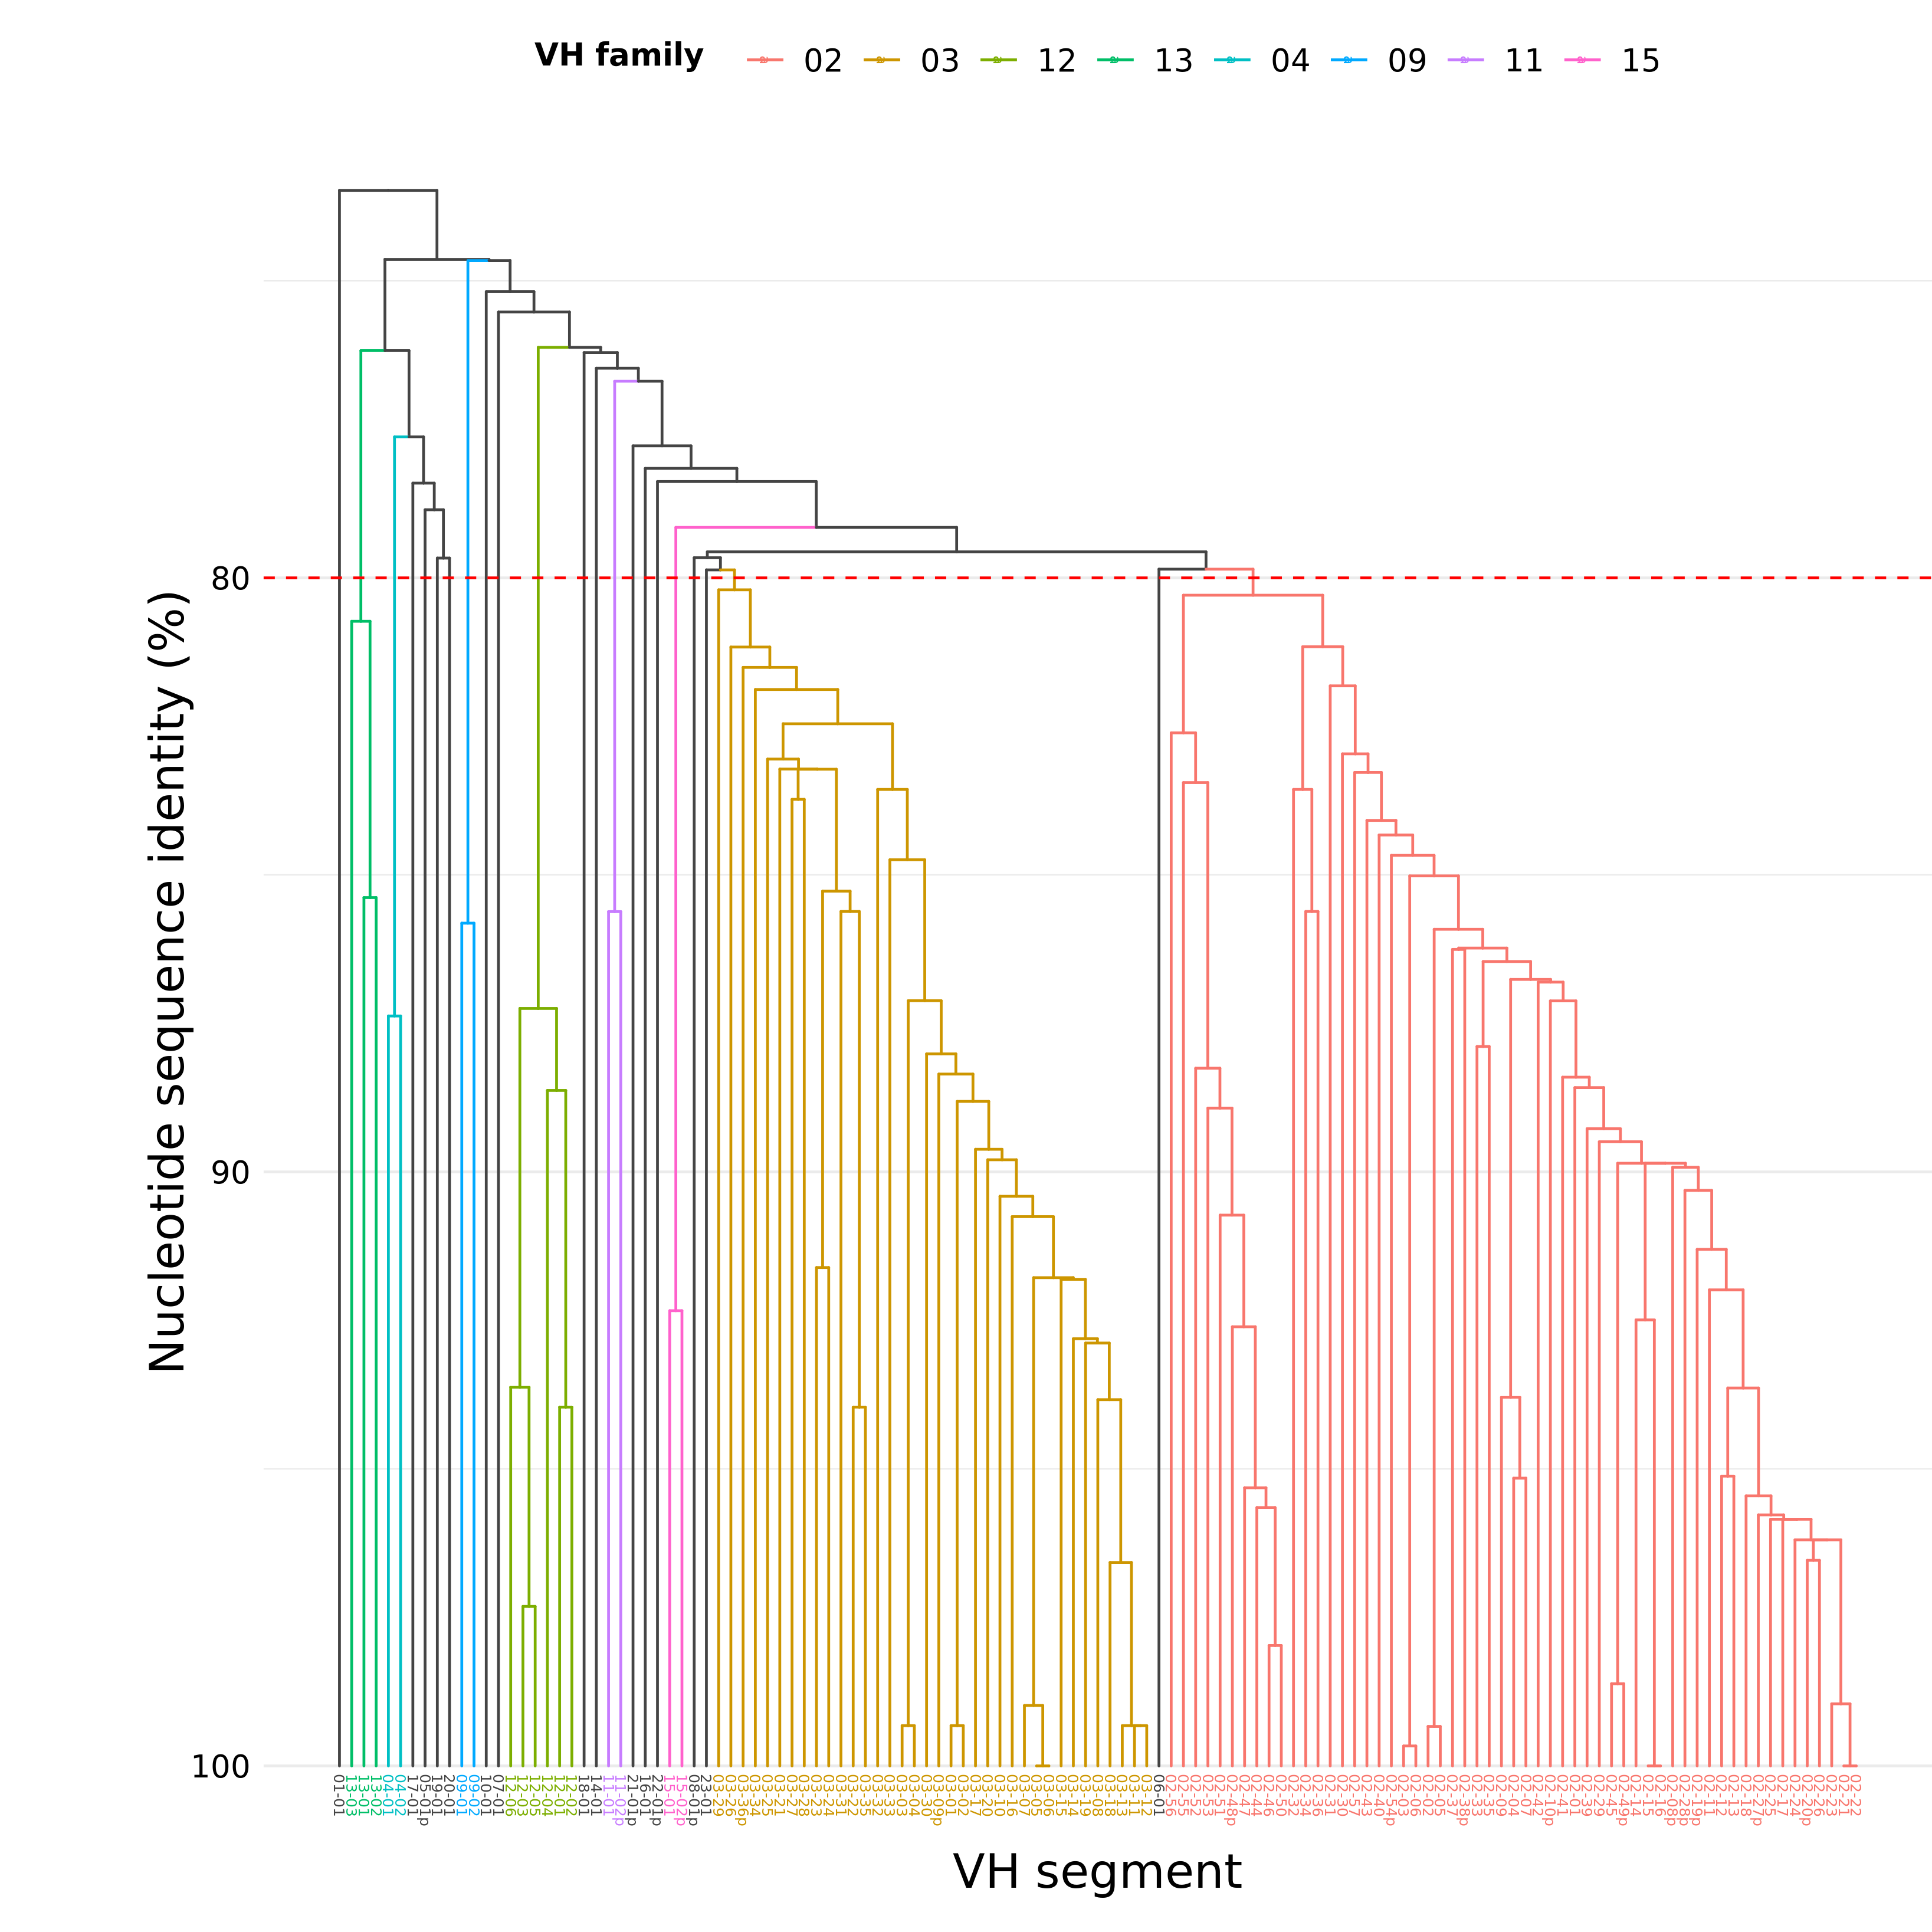
\includegraphics[width=\textwidth]{_Figures/png/xma-vh-families-tree}
	\Caption{Dendrogram of \vh families in the \Xma \igh{} locus}{Dendrogram of sequence similarity of \vh segments in the \Xma locus, arranged by single-linkage clustering on nucleotide sequence identity. The red line indicates the 80\,\% cutoff point for family assignment, while branch colour indicates family membership:  \vh families containing multiple segments are uniquely coloured, while single-segment families are in grey.}
	\label{fig:xma-vh-families-tree}
	\end{figure}
	
	\begin{figure}
	\centering
	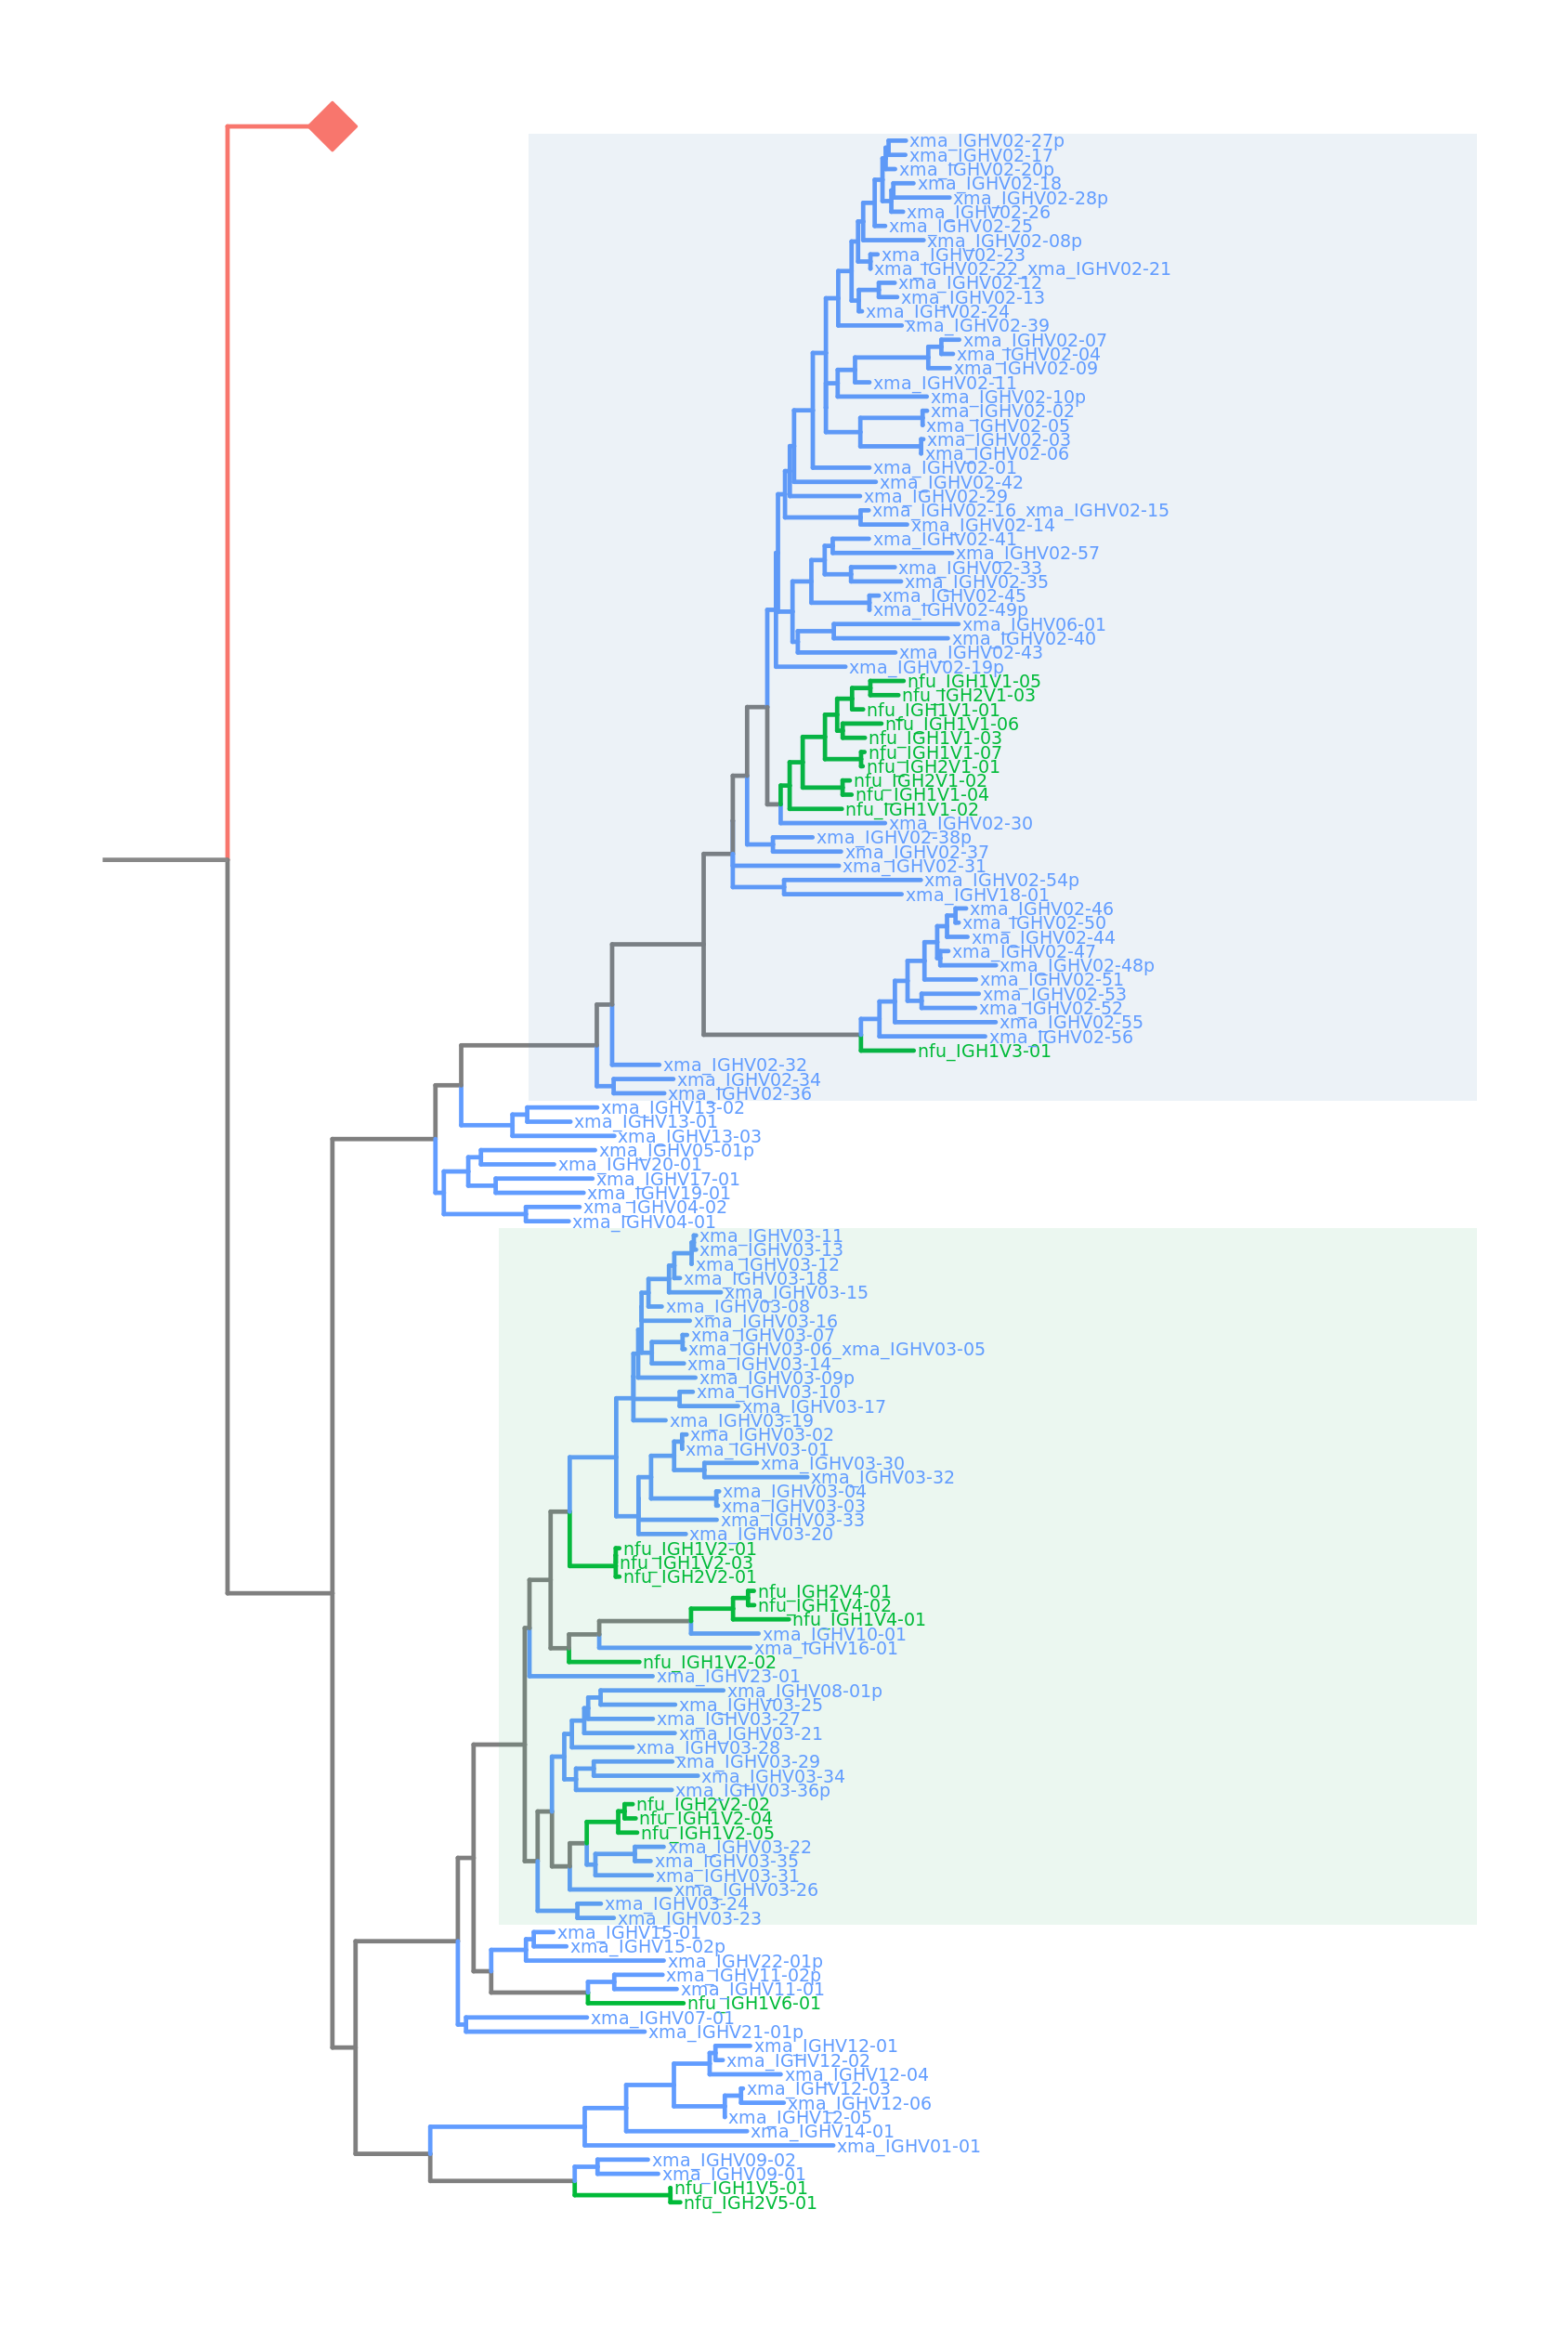
\includegraphics[width=0.8\textwidth]{_Figures/png/nfu-xma-vh-tree-nt.png}
	\Caption{Evolutionary relationships between \vh families in \Xma and \Nfu}{Phylogenetic tree of evolutionary relationships between \igh{} \vh segments in \Nfu and \Xma, as inferred from the nucleotide sequences of \vh segments from both loci. Note the close interrelationship between the largest \vh families in each species (red zone), and similarly between the second-largest families in each species (blue zone). The red diamond indicates the location of the outgroup, which is composed of zebrafish \textit{TRB} V-segments.}
	\label{fig:nfu-xma-vh-tree-nt}
	\end{figure}
		
\FloatBarrier

\clearpage

\section{\igh{} constant-region evolution in the Cyprinodontiformes}
\label{sec:locus_comparative}

The characterised \igh{} loci of \nfu and \xma together reveal a high degree of variability in structure and function across the Atherinomorpha, the parent clade of the Cyprinidontiformes (including \Nfu and \Xma) and medaka (\Cref{fig:species-tree-large-taxa}). Several unusual features (including the loss of \igh{Z}, an inverted sublocus, and an unusual splicing pattern of \igh{M-TM}) are shared between medaka and turquoise killifish, but absent in \Xma (\Cref{fig:species-tree-small}), indicating either an independent origin in the former two species or a reversion to the primitive state in the latter. In addition, the copy number, exon usage and orientation of constant regions of other isotypes differs among the three species, raising the further question of how, when and why these changes occurred. 

In order to investigate a subset of these questions with a greater degree of phylogenetic resolution, I identified and analysed \igh{} constant regions in the genomes of ten additional cyprinodontiform species (\Cref{fig:species-tree-large-taxa}, \Cref{tab:cyprinodontiform-genomes}), as well as in a new and improved genome assembly of medaka (Genbank accession GCA\_002234675.1), using the same methods described for \Nfu and \Xma (\Cref{sec:nfu-locus-constant,sec:nfu-locus-variable}). I then grouped the constant-region exons so identified (\Cref{fig:ch-tree-all}) by order, exon type and spatial proximity to identify contiguous constant-regions, enabling the presence/absence and number of constant regions of each isotype to be estimated for each species. The results of this analysis (\Cref{fig:multispecies-ch-regions}, \Cref{tab:multispecies-ch-regions-1,tab:multispecies-ch-regions-2,tab:multispecies-ch-regions-3}) demonstrate that every species investigated possesses at least one complete \igh{M} and \igh{D} constant region in tandem, with several species exhibiting multiple such regions. Apart from \Nfu and medaka, only \textit{Nothobranchius orthonotus} was identified as clearly possessing adjacent constant regions in opposite orientation, indicating the presence of at least one sublocus in antisense; however, the fragmented nature of the \igh{} locus assembly in many analysed species prevented a confident exclusion of such configurations in other cases.

\begin{table}[bh!]
\centering
\begin{threeparttable}
\begin{tabular}{>{\itshape}l>{\itshape}llc}\toprule
\textnormal{\textbf{Genus}} & \textnormal{\textbf{Species}} & \textbf{Common Name} & \textbf{GenBank Assembly Accession}\\\midrule
Nothobranchius & furzeri & Turquoise killifish & NA\tnote{1}\\\midrule
Xiphophorus & maculatus & Southern platyfish & GCA\_002775205.2\\
Austrofundulus & limnaeus & -- & GCA\_001266775.1\\
Fundulus & heteroclitus & Mummichog & GCA\_000826765.1\\
Poecilia & formosa & Amazon molly & GCA\_000485575.1\\
Poecilia & reticulata & Guppy & GCA\_000633615.1\\
Cyprinodon & variegatus & Sheepshead minnow & GCA\_000732505.1\\
Kryptolebias & marmoratus & Mangrove rivulus & GCA\_001649575.1\\\midrule
Aphyosemion & australe & Lyretail panchax & NA\tnote{2}\\
Callopanchax & toddi & -- & NA\tnote{2}\\
Pachypanchax & playfairii & Golden panchax & NA\tnote{2}\\
Nothobranchius & orthonotus & Spotted killifish & NA\tnote{2}\\\midrule
Oryzias & latipes & Medaka & GCA\_002234675.1\\
\bottomrule\end{tabular}
\begin{tablenotes}
\item[1] Willemsen \textit{et al.} \parencite{willemsen2019popgen}
\item[2] Cui \textit{et al.} \parencite{cui2019annual}
\end{tablenotes}
\end{threeparttable}
\vspace{0.5em}
\caption{Genome assemblies used to identify \igh{} locus sequences in cyprinodontiform fishes}
\label{tab:cyprinodontiform-genomes}
\end{table}

\begin{figure}
\centering
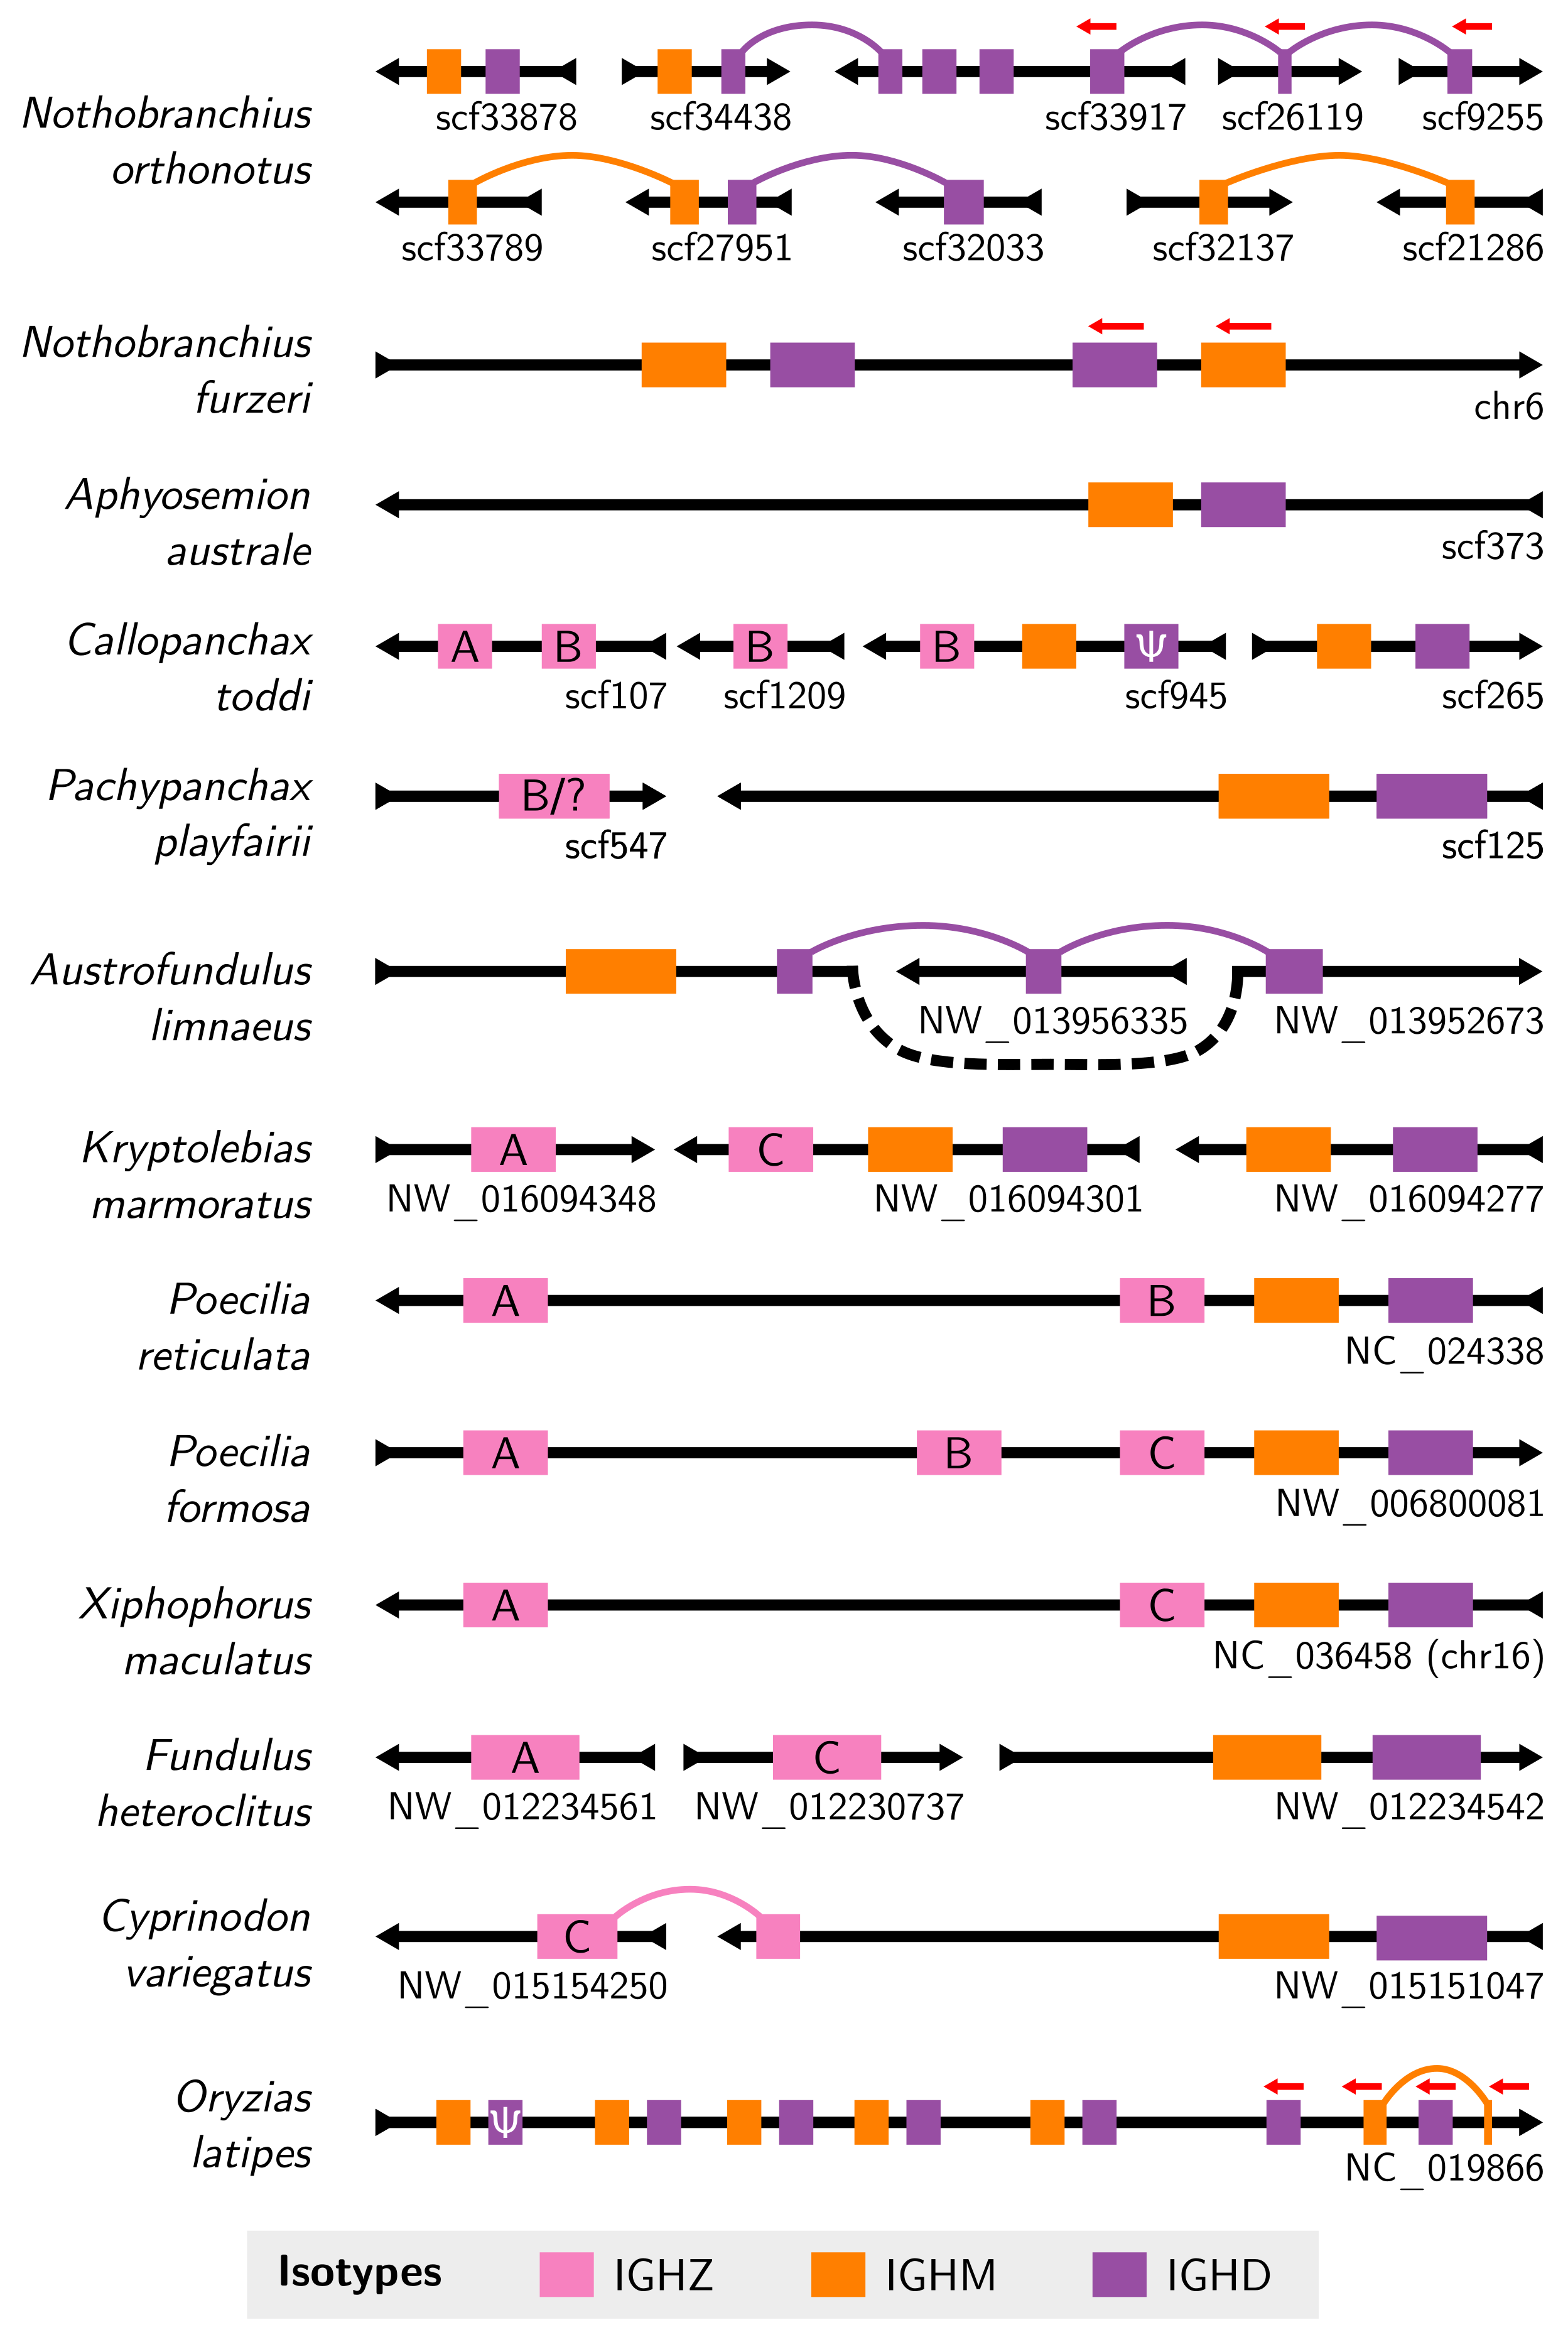
\includegraphics[width=0.9\textwidth]{_Figures/png_edited/multispecies-ch-regions}
\Caption{Constant-region organisation in the Atherinomorpha}{Schematic of \igh{} constant regions in the genomes of thirteen species from the Atherinomorpha. Scaffold orientation is given by the black arrows; constant regions are oriented left-to-right unless otherwise specified (red arrows). Links between regions on different scaffolds indicate that exons from what appears to be the same constant region are distributed across multiple scaffolds in the order indicated; the order of unlinked scaffolds is arbitrary. The isotype of each region is given by its colour; \igh{Z} regions are further annotated with their subclass (\Cref{fig:species-tree-large-ighz}). Clearly pseudogenised constant regions are indicated by $\Psi$. Isotype length, scaffold length, and scaffold position are not to scale. Variable regions and lone, isolated constant-region exons are not shown.}
\label{fig:multispecies-ch-regions}
\end{figure}

In addition to at least one \igh{M} and \igh{D} constant region, the majority of species analysed (8 out of 13) were also found to possess at least one complete \igh{Z} constant region; of the exceptions, \species{A.}{limnaeus} exhibits an orphaned, pseudogenised \igh{Z-TM1} exon but no \cz{} exons in the current genome assembly (\Cref{fig:multispecies-ch-regions}, \Cref{tab:multispecies-ch-regions-2}), while \species{O.}{latipes}, \species{A.}{australe}, \Nfu and \species{N.}{orthonotus} possess no \igh{Z} exons at all. Annotating the tree from \Cref{fig:species-tree-large-taxa} with the \igh{Z} status of each species (\Cref{fig:species-tree-large-ighz}) confirms that the loss of \igh{Z} in turquoise killifish (and related species) and medaka represent two distinct deletion events, with \textit{Austrofundulus limnaeus} potentially representing a second independent loss of \igh{Z} within the Cyprinodontiformes and a third within the Atherinomorpha.

\begin{figure}
\centering
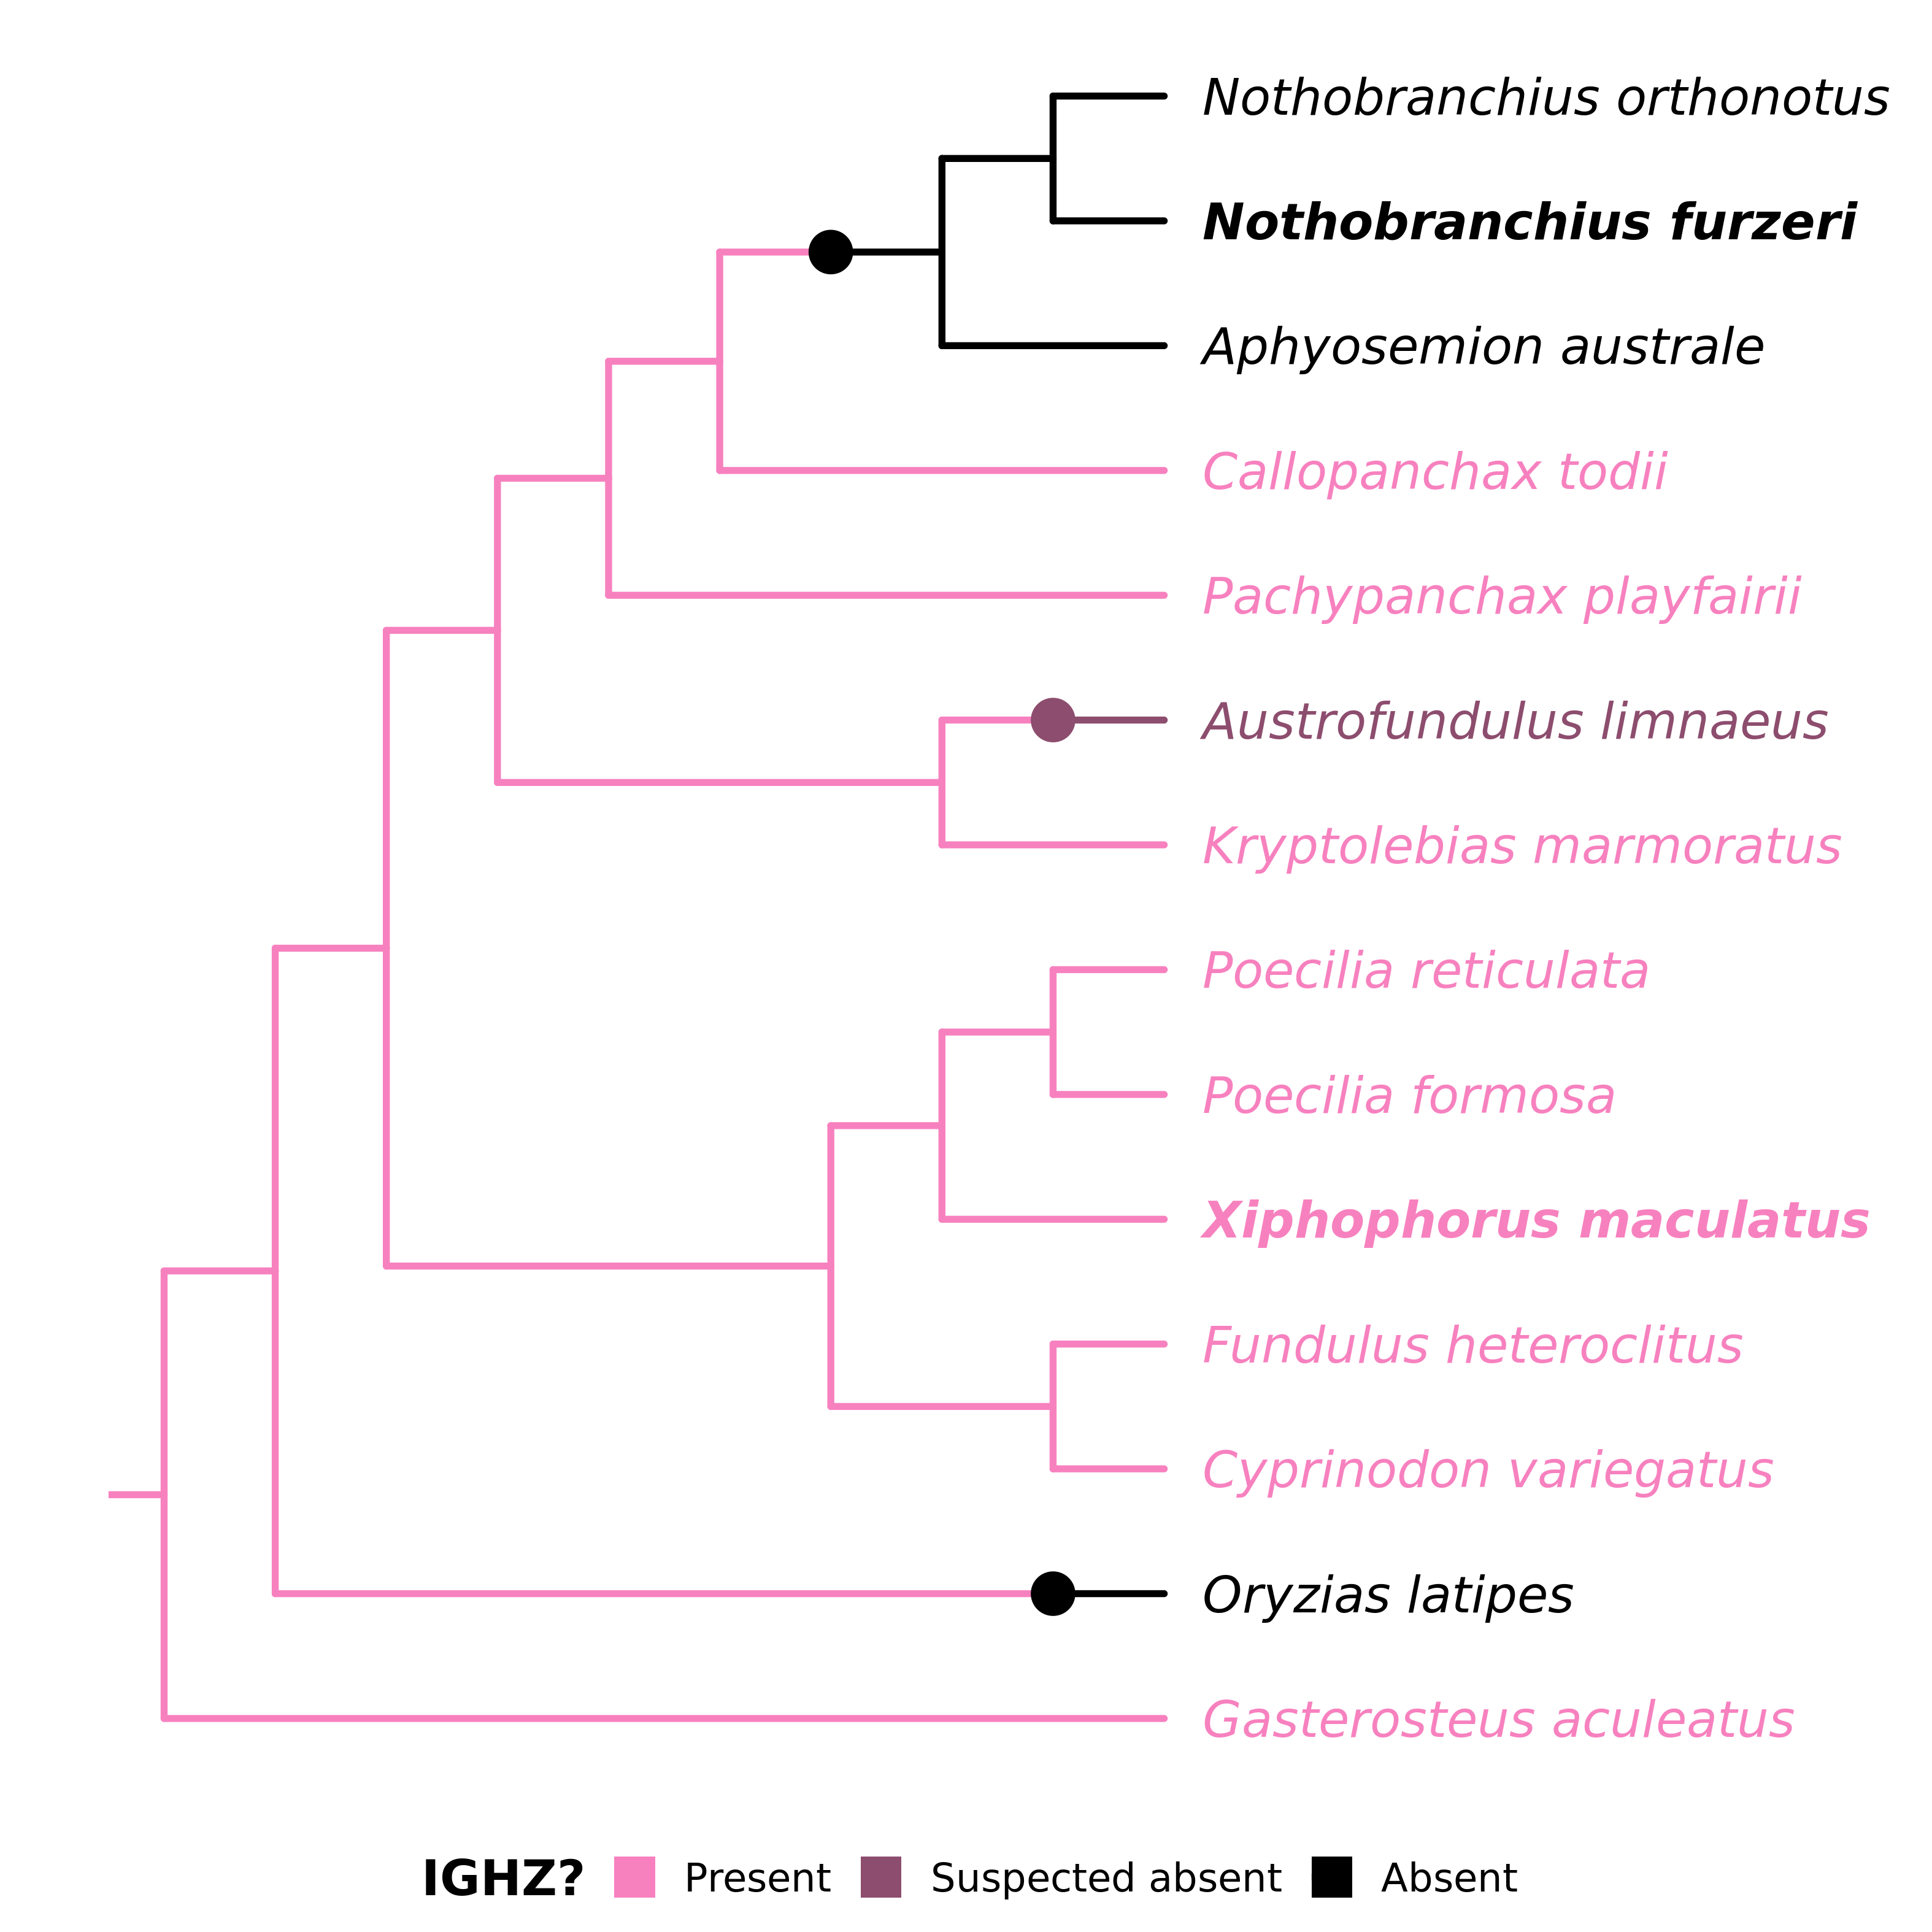
\includegraphics[width=0.9\textwidth]{_Figures/png/species-tree-large-ighz}
\Caption{\igh{Z} has been lost multiple times independently in the Atherinomorpha}{Cladogram of species reproduced from \Cref{fig:species-tree-large-taxa}, annotated according to the known (tip nodes) or inferred (internal nodes) presence or absence of intact \igh{Z} constant regions in each species. Large coloured points on the cladogram denote sites of hypothesised state changes; \igh{Z} is assumed to be primitively present in the clade and losses to be irreversible. The currently-available genome assembly of \textit{A. limnaeus} (dark pink) contains one pseudogenised \igh{Z-TM1} exon and no \cz{} exons.}
\label{fig:species-tree-large-ighz}
\end{figure}

Apart from its repeated loss within the lineage, a second striking feature of \igh{Z} within the Cyprinodontiformes is its frequent presence in multiple copies per \igh{} locus, with a geometric mean of 1.929 regions per \igh{Z}-bearing locus. On average (geometric mean), the species analysed have approximately 1.62 \igh{Z} constant regions per \igh{M} constant region, and the same ratio vs \igh{D}, suggesting a more complex evolutionary history than can be captured by a simple presence/absence metric. Concordantly, phylogenetic analysis (\Cref{fig:multispecies-cz-tree}, tree built using \program{PRANK} and \program{RAxML} on concatenated \cz{1}--\cz{4} exon sequences) reveals three distinct lineages (or subclasses) of \igh{Z} constant regions in the Cyprinidontiformes, \igh{ZA} to \textit{C}, each of which is present in multiple different species and appears to have been present in the common ancestor of the eight \igh{Z}-bearing species analysed (\Cref{fig:multispecies-cz-subclasses}).

\begin{figure}
	\centering
	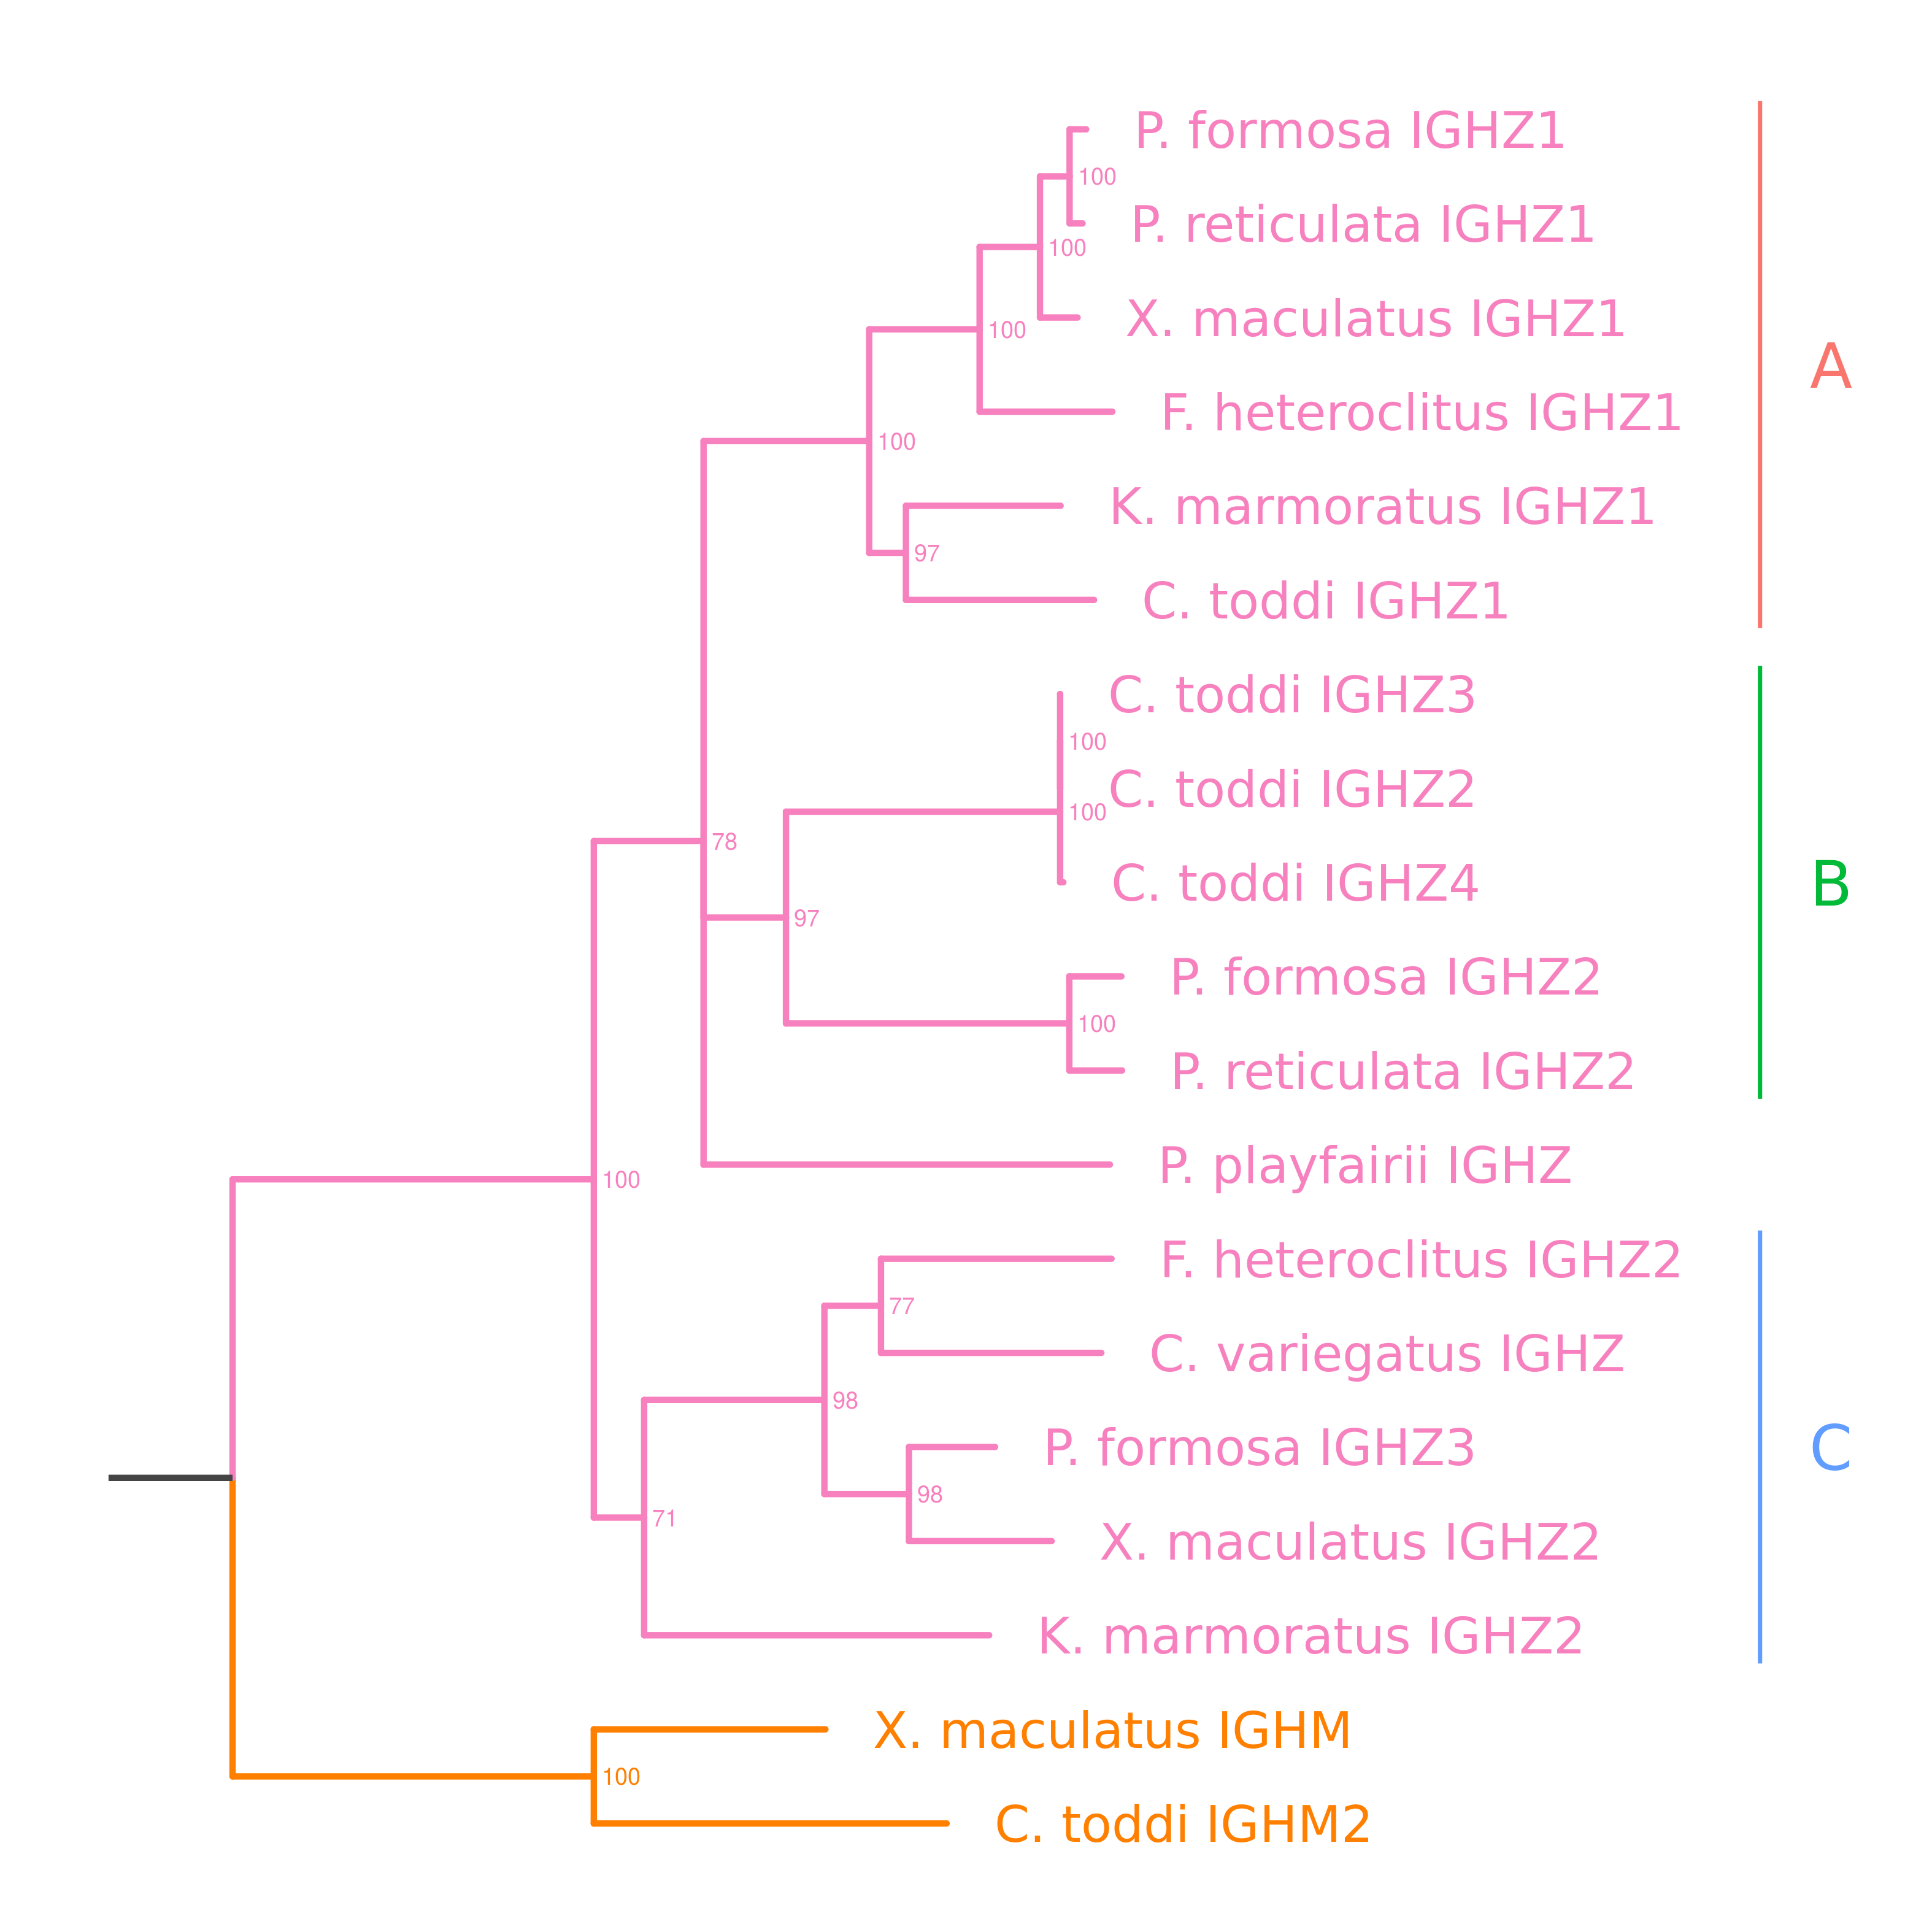
\includegraphics[width=0.9\textwidth]{_Figures/png/multispecies-cz-tree}
	\Caption{\igh{Z} constant regions in the Cyprinodontiformes constitute three distinct subclasses}{Phylogram of concatenated \cz{1}--\cz{4} nucleotide sequences from \igh{Z}-bearing species in \Cref{tab:cyprinodontiform-genomes}, with \cm{1}--\cm{4} sequences from two species as an outgroup (in orange). Nodes with bootstrap support of less than 65\,\% are collapsed into polytomies. Major clades (A--C) are annotated on the right. Support values indicate the result of rapid bootstrapping by \program{RAxML} across 1000 replicates.}
	\label{fig:multispecies-cz-tree}
\end{figure}

\begin{figure}
\centering
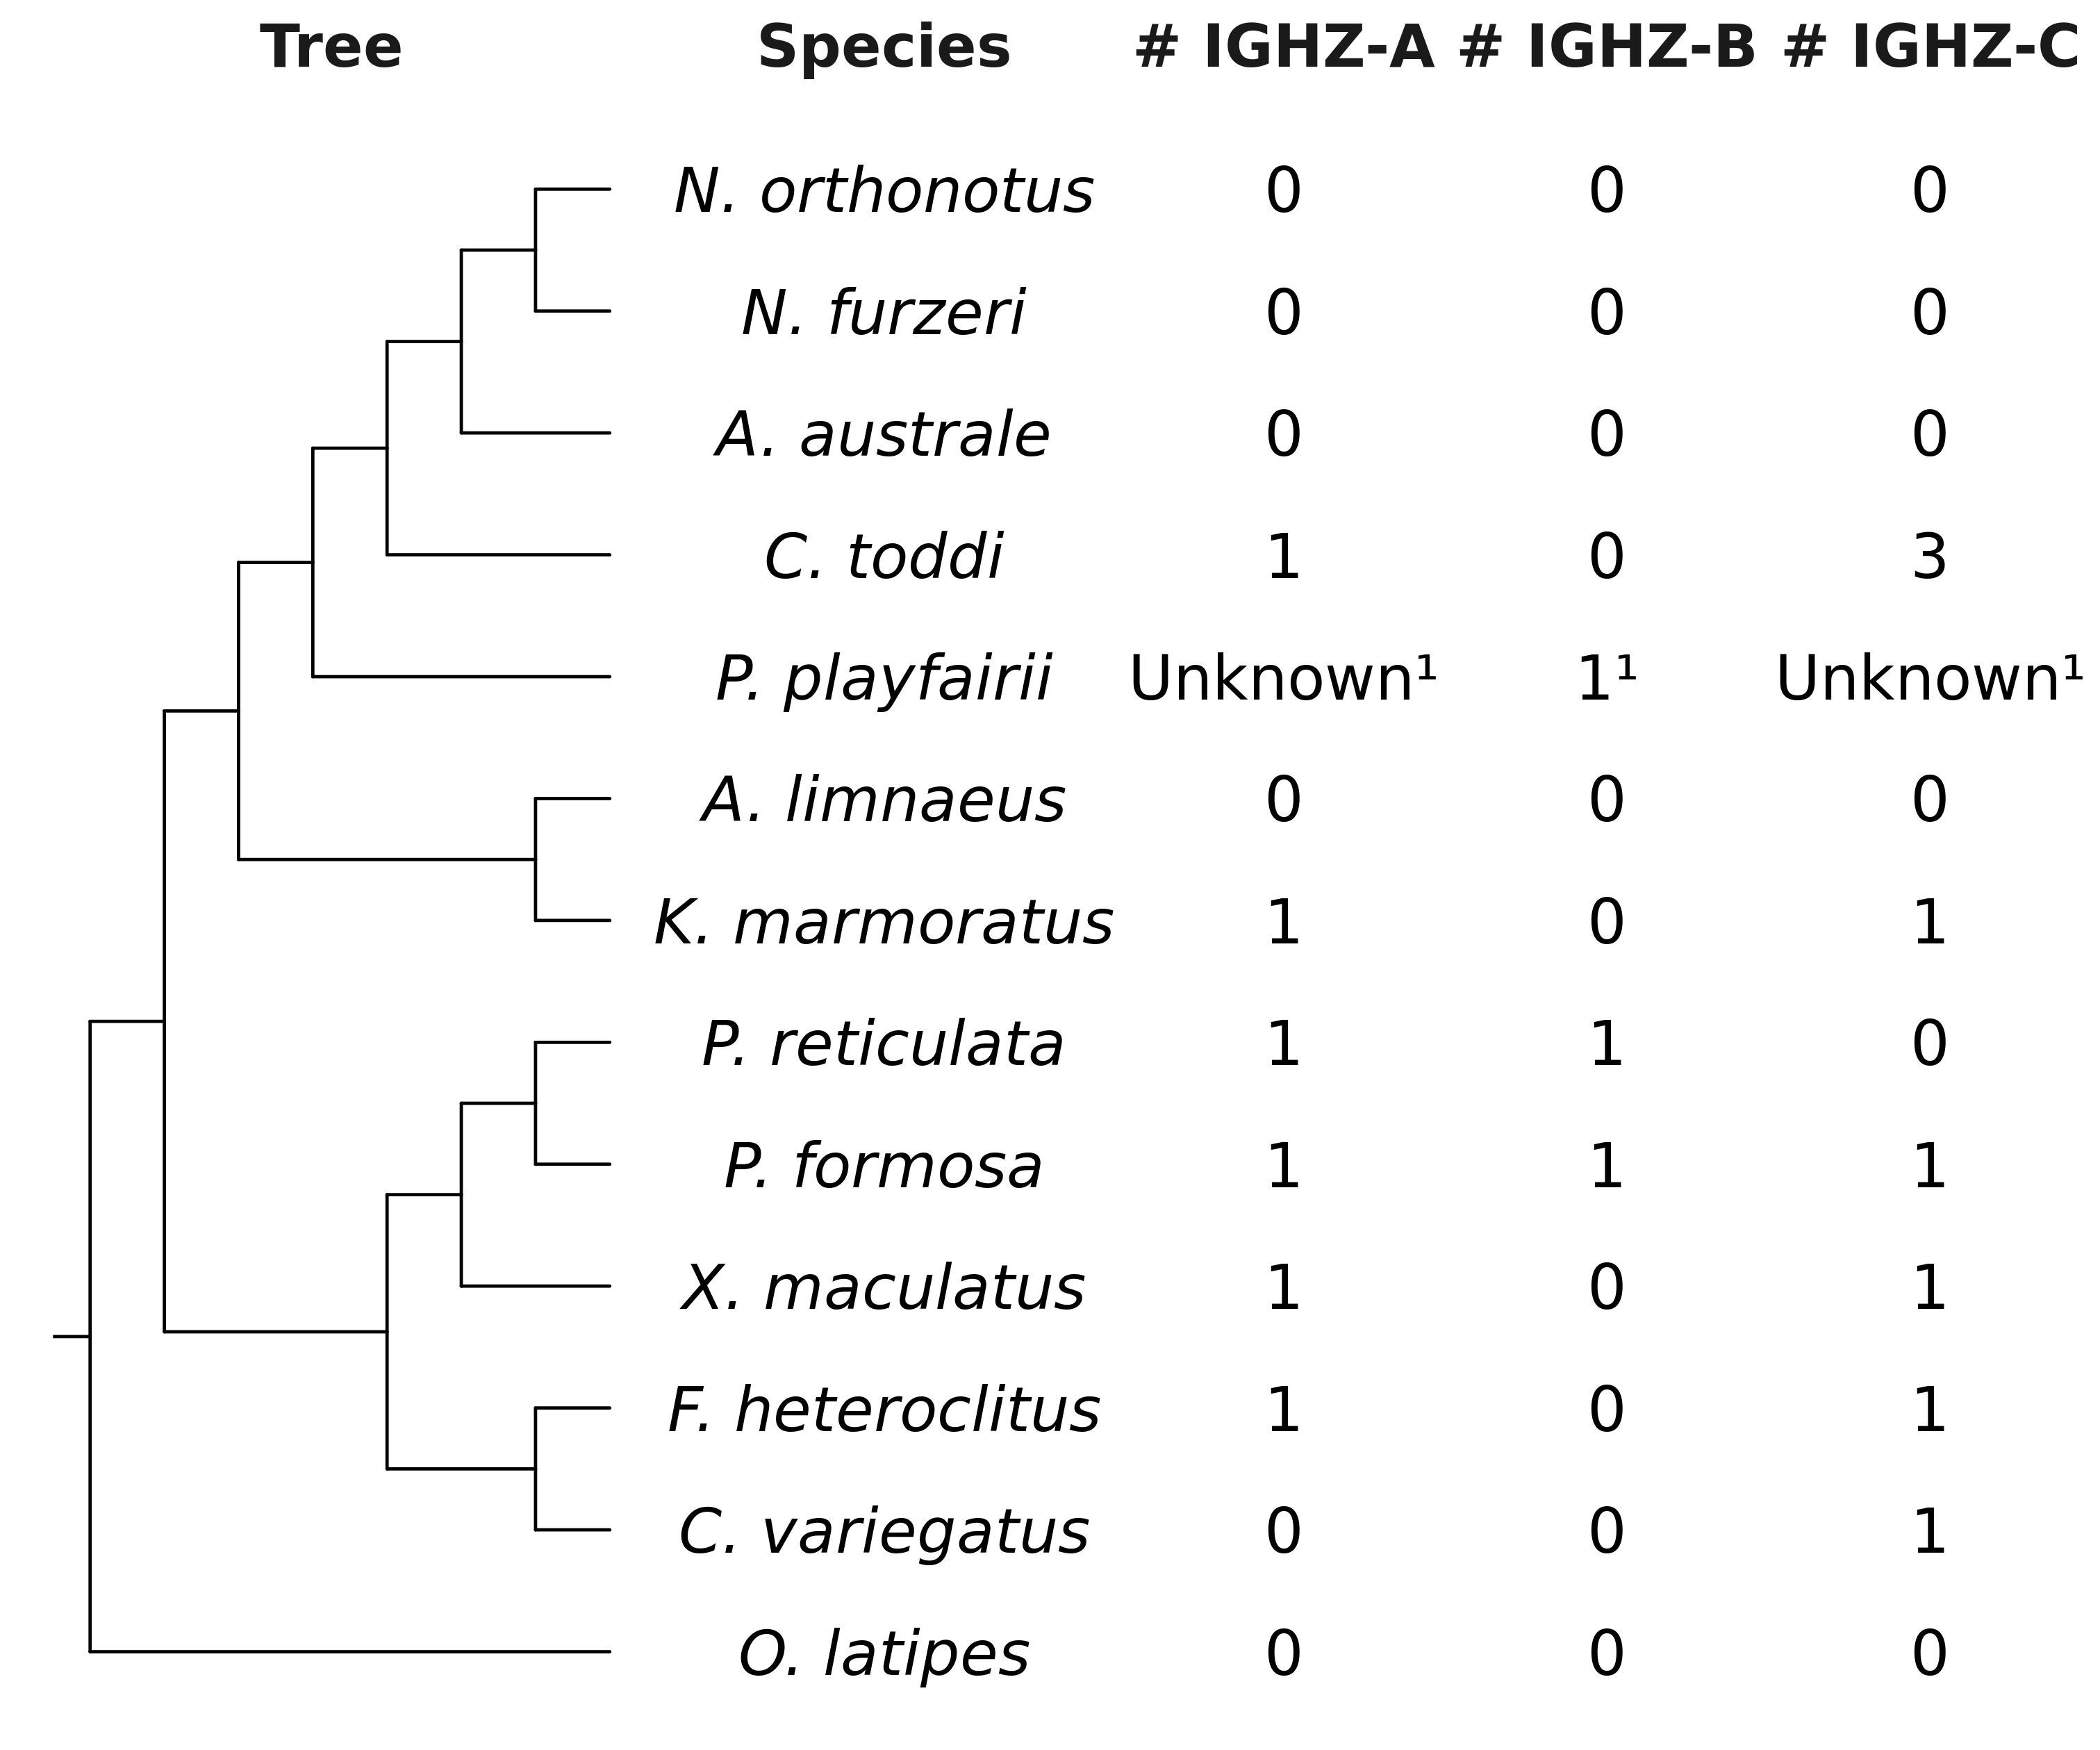
\includegraphics[width=0.8\textwidth]{_Figures/png/multispecies-cz-subclasses}
\begin{minipage}{0.7\textwidth}
\footnotesize
\begin{threeparttable}
\begin{tablenotes}
\item[1] \textit{P. playfairii} \igh{Z} \cz{1}--\cz{2} appear to be derived from \igh{Z-B}, while the other exons are of uncertain subclass origin (\Cref{fig:ppl-cz-aln}).
\end{tablenotes}
\end{threeparttable}
\end{minipage}
\Caption{Distribution of \igh{Z} subclasses in the Atherinomorpha}{Cladogram of atherinomorph species with characterised \igh{} constant regions, annotated with the number of regions belonging to each \igh{Z} isotype in each species. All three subclasses are present in at least one species in both major branches of the cyprinodontiform clade, suggesting that they were all present in the common ancestor of this grouping.}
\label{fig:multispecies-cz-subclasses}
\end{figure}


Only one \igh{Z} constant region from the analysed species could not be confidently assigned to one of these three subclasses, namely the single \igh{Z} of \species{Pachypanchax}{playfairii} (\Cref{fig:multispecies-cz-tree}). In order to more closely investigate the relationships of \igh{Z} in this species, I aligned the exon sequences of \species{P.}{playfairii} \cz{1}--\cz{4} separately to the \cz{} exons of all other \igh{Z}-bearing species and plotted the distribution of alignment scores in each case (\Cref{fig:ppl-cz-aln}). The results show a striking difference in alignment behaviour between the exons, with \cz{1} and \cz{2} aligning significantly more strongly to exons from the B subclass and \cz{3} and \cz{4} showing more ambiguous affinity for either A- or C-subclass sequences. This unexpected behaviour indicates that the \species{P.}{playfairii} \igh{Z} sequence is the result of a deletion or fusion event combining the first two exons of a B-subclass \igh{Z} constant region with the latter exons of a constant region from another subclass, resulting in a chimeric gene with ambiguous ancestry.

\begin{figure}
	\centering
	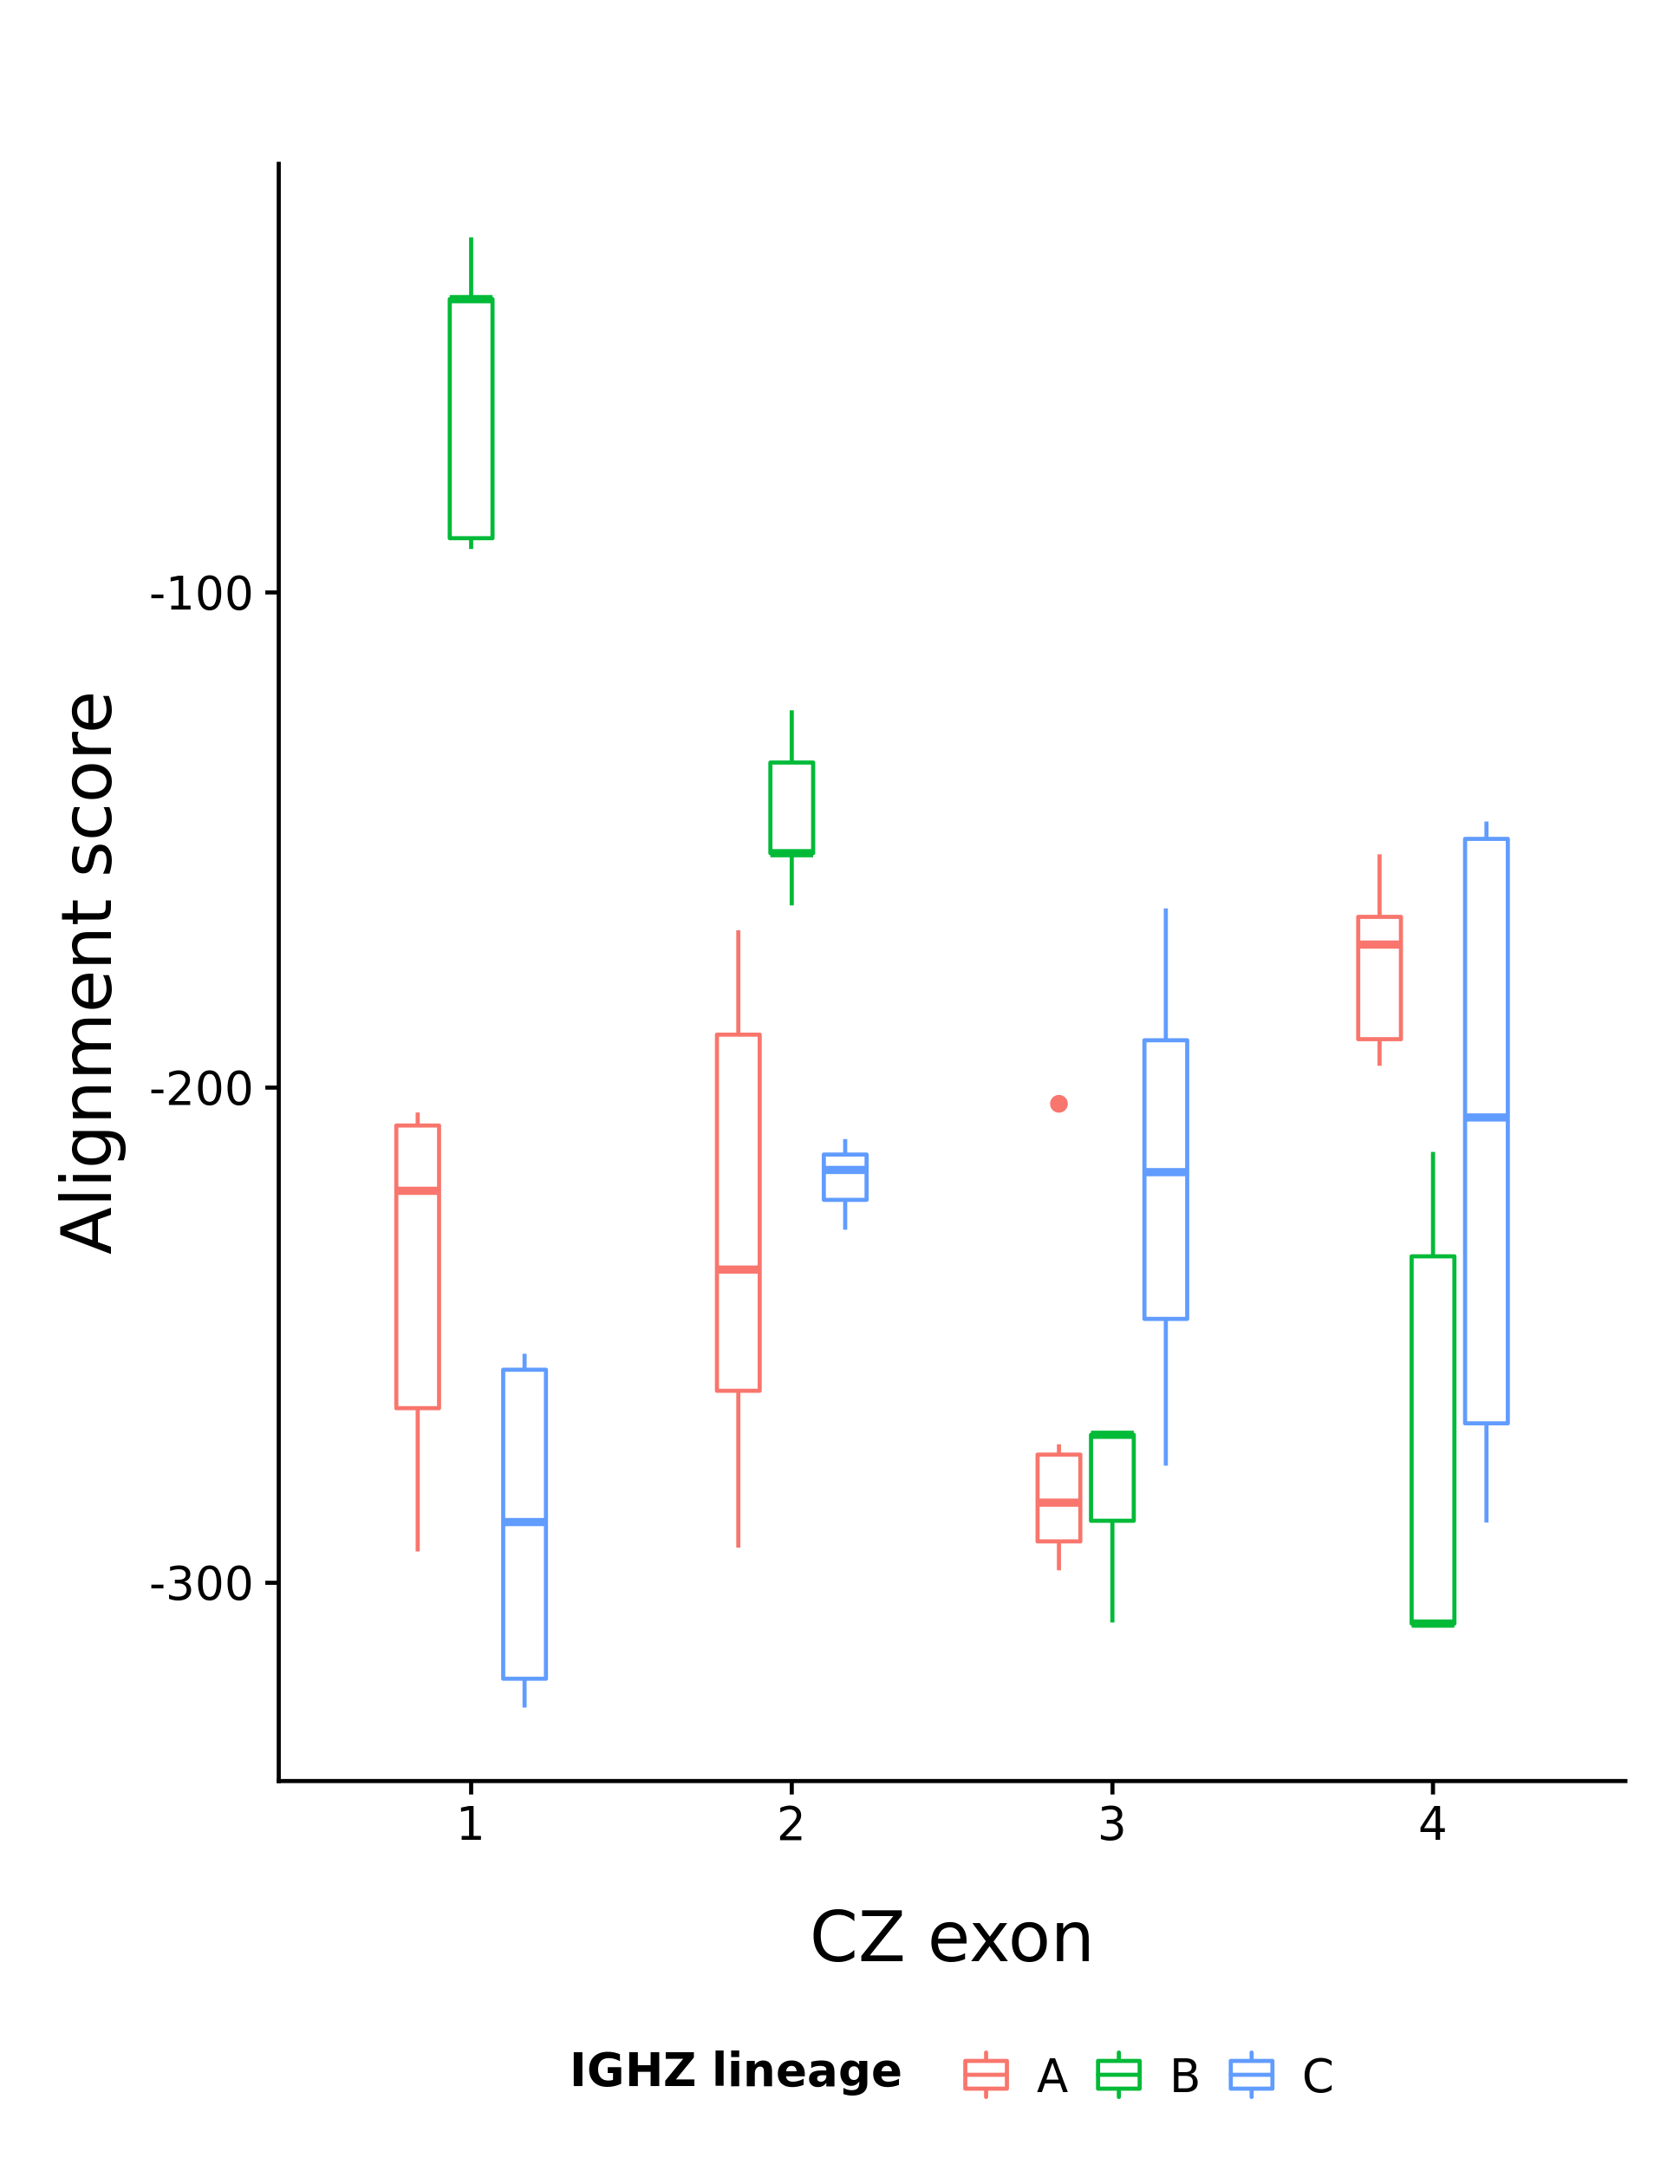
\includegraphics[width=0.8\textwidth]{_Figures/png/ppl-cz-aln-aa.png}
	\Caption{Subclass affinity of \igh{Z} in \species{Pachypanchax}{playfairii}}{Boxplots of Needleman-Wunsch alignment scores between the amino-acid sequences of \species{P.}{playfairii} \cz{} exons and those of seven other \igh{Z}-bearing cyprinodontiform species, demonstrating the differing affinity of different \species{P.}{playfairii} exons for each of the three \igh{Z} subclasses. Pairwise $p$-values were computed using nonparametric Mann-Whitney $U$ tests ($*: 0.01 < p \leq 0.05;~**: 0.001 < p \leq 0.01;~***: p \leq 0.001$).}
	\label{fig:ppl-cz-aln}
\end{figure}
	
In summary, in addition to the still-universal primitive antibody classes \igh{M} and \igh{D}, the cyprinodontiforms ancestrally possessed at least three variants of \igh{Z}, giving rise to multiple subclasses of \igh{Z} constant regions evolving in parallel across the clade. Each of these subclasses appears to have been lost in multiple cyprinodontiform species, with different species showing distinct patterns of retention and loss, and in at least one lineage -- that of \species{Pachypanchax}{playfairii} -- two different \igh{Z} lineages have fused to produce a chimeric isotype. All three subclasses are missing from a subset of species in the Nothobranchiidae (including \nfu), and also appear to have been independently lost in \species{Austrofundulus}{limnaeus}. Taken together, these data suggest a high degree of complexity and volatility in the evolution of mucosal adaptive immunity in the Cyprinodontiformes.

\newpage

\section{Discussion}

The teleost fishes are the largest and most diverse group of vertebrates, with nearly 30,000 species comprising almost half of extant vertebrate diversity \parencite{ravi2018divergent}. Of this vast variety of teleosts, only a few species, mostly those used extensively in aquaculture or scientific research, have undergone extensive study with regard to their immunoglobulin gene loci (\Cref{sec:intro_teleost_loci}). Studies in these model species have revealed a high level of structural diversity among teleost \igh{} loci, with huge variation in both size and organisation, as well as the existence of three distinct antibody isotypes in fish, of which two (\igh{M} and \igh{D}) are shared with tetrapods and one (\igh{Z}) appears to be teleost-specific. However, in many large and important teleost lineages, the genetic basis of B-cell-mediated humoral immunity remains unknown.

In this chapter, I presented two complete and ten partial assemblies of \igh{} loci from the Cyprinodontiformes, a diverse clade of primarily freshwater fishes for which no such loci have previously been characterised. The two complete assemblies were of the \igh{} loci of the turquoise killifish \nfu and the southern platyfish \xma, two important model species with an estimated divergence time of less than 80 Mya \parencite{hughes2018teleostphylo}. Despite their close relationship, these species show radically different locus organisations, with huge differences in VDJ number (24 \vh segments in \Nfu versus 125 in \Xma), locus organisation (two small subloci in opposite sense in \Nfu, one large unitary locus in \Xma) and isotype availability (no \igh{Z} in \Nfu, two distinct \igh{Z} regions in \Xma), as well as more subtle but still-important distinctions like differences in constant-region splicing behaviour (four exons in \Nfu \igh{M-TM}, five in \Xma). These results are consistent with previous findings of highly-diverse teleost loci and support a process of rapid evolution in the \igh{} locus. Characterisation of the constant regions of a further ten cyprinodontiform species confirmed this finding, with several groups of closely-related species (e.g. \nfu, \species{Nothobranchius}{orthonotus} and \species{Callopanchax}{toddi}) showing highly divergent locus structures and constant-region availability.

It is interesting to speculate on the origins of this extremely rapid diversification in gene structure. Very little is known about the relationship between environmental context and immune locus structure; it is possible that part of the variety in \igh{} gene locus structure in the Cyprinodontiformes represents divergent adaptations to different immune environments. Alternatively, this diversification may be primarily the result of unusually high rates of stochastic, non-adaptive changes in gene structure in germline \igh{}. Finally, at least some of the difference between locus structures in different species is likely to be attributable to differences in assembly quality; for example, the characterisation of medaka constant regions presented here contains many fewer unusual or incomplete constant regions than that presented in the published medaka \igh{} locus \parencite{magadan2011medaka}, primarily due to the increased quality of the more recent medaka genome assemblies.

Before the publication of this work, only two teleost species (medaka and channel catfish) were known or thought to lack the \igh{Z} antibody isotype from their \igh{} loci, out of more than ten species with published locus characterisations. This relative rarity of observed absence, combined with the apparent importance of \igh{Z} in teleost mucosal immunity, suggested that the loss of \igh{Z} was likely to be a rare and unusual event. However, in addition to confirming the absence of \igh{Z} in medaka, this study identified four new teleost species (\nfu, \species{Nothobranchius}{orthonotus}, \species{Aphyosemion}{australe} and \species{Austrofundulus}{limnaeus}) that appear to lack \igh{Z} constant regions in their \igh{} loci, representing two distinct and previously unknown loss events independent from that affecting the closely-related medaka. This finding, which triples the number of known teleost species without \igh{Z} and doubles the number of known loss events, is even more striking when combined with the discovery that the cyprinidontiform common ancestor likely had no fewer than three distinct \igh{Z} constant regions, all of which would have had to be lost on the way to any \igh{Z}-free lineage. The high level of observed variability in \igh{Z} prevalence among the cyprinidontiforms suggests that the presence/absence of \igh{Z} in the wider teleost clade may be much more volatile than suggested by previously available locus data, and raises the possibility that, given sufficiently high-density analysis of other teleost lineages, a similar frequency of \igh{Z}-lacking species may also be found elsewhere. However, it may also be the case that the apparently high frequency of \igh{Z} loss events in the Atherinomorpha is a special case, arising from chance, an unusual selective environment, or limitations in the available genome assemblies.

The absence of \igh{Z} from so many species in the Atherinomorpha naturally raises the important question of how the mucosal adaptive immune system in these species differs from that of their \igh{Z}-bearing relatives. Data from rainbow trout suggest that \igh{T} (an alternative name for \igh{Z} in some species) plays a specialised role in antibody immune responses at multiple mucosal surfaces, with increased prevalence of \igh{T}$^+$ B-cells and secreted IGHT antibodies relative to serum, a primarily \igh{T}-dependent response to mucosal infections, and a much higher rate of bacterial coating by IGHT in skin and gut flora relative to IGHM \parencite{zhang2010igtgut,xu2013igtskin}.
If these findings hold for other teleost species, it is not clear how \igh{Z}-lacking teleost species carry out specialised immune functions at mucosal barriers: how, and to what extent, can \igh{M} compensate for the loss of a specialised mucosal isotype? This question is especially interesting in the case of \igh{Z}-lacking species with close \igh{Z}-bearing relatives (e.g. \nfu and \species{Callopanchax}{toddi}, or perhaps \species{Austrofundulus}{limnaeus} and \species{Kryptolebias}{marmoratus}); if it is the case that mucosal immune responses differ systematically between these species, such that \igh{M} takes up some or all of the roles normally played by \igh{Z}, then uncovering the mechanisms by which this shift is regulated could reveal important new insights into decision-making and control of humoral adaptive immunity.

One important difference between the \Xma and \Nfu loci whose evolution is more difficult to investigate using genomic data is the exon usage behaviour of the different splice isoforms present in the transcriptome of each species. In \Xma, transmembrane \igh{M} adopts the same configuration as that seen in most teleosts for which this has been investigated: a five-exon isoform in which the end of \cm{3} is spliced to the start of TM1 and \cm{4} is excised. Conversely, in \Nfu \igh{M-TM} adopts the same four-exon configuration observed in medaka, in which \cm{3} is also excluded. Given that \Xma adopts the primitive configuration, the recurrence of the same unusual configuration in both medaka and turquoise killifish is surprising, and indicates that both configurations are present in the Cyprinodontiformes; however, without more information about the mechanisms and genomic sequence correlates underlying this difference, it is impossible to distinguish an independent origin of the derived phenotype in medaka and \Nfu from a reversion to the primitive phenotype in \Xma. It is also not clear at present what functional differences, if any, arise from this difference in exon usage, although it seems unlikely that the shorter four-exon form of \igh{M-TM} would persist in multiple species if it prevented effective antibody development, selection, or antigen response.

As a result of the research findings presented in this chapter, a number of previously-uncharacterised teleost species now have databases of constant regions available. As a result, primer design for targeted RNA-sequencing of expressed antibody sequences is now possible for these taxa, enabling quantitative immune-repertoire sequencing approaches in a large number of closely-related cyprinidontiform species. In addition to the special interest of immune-repertoire data from any one of these new species (e.g. \Nfu for immune-repertoire ageing or \Xma for ecological and evolutionary research), the possibility of sequencing the repertoires of several related species adds an exciting comparative dimension. This comparative element would be especially interesting in the context of investigating the repertoire responses of closely related species with different \igh{Z} genotypes. In combination with the genomic and functional comparisons discussed above, the novel possibility of large-scale comparative repertoire studies arising as a result of this research establishes the Cyprinidontiformes, and especially the African killifishes, as a highly-promising group of model species for comparative evolutionary immunology.

% TODO: Ask Dario re discussion

\chapter{Immunoglobulin sequencing in \textit{Nothobranchius furzeri}} 
\label{chap:igseq} 
\onehalfspacing

\pagebreak

\section{Introduction}
\label{sec:igseq_intro}

The antibody repertoire of an individual is the complete collection of immunoglobulin sequences (either DNA, RNA or protein) expressed or secreted by the complete population of B-lymphocytes it contains \parencite{miho2018computational}. This enormous population of sequences contains both a high degree of sequence diversity and a great deal of functionally-relevant internal structure: \naive sequences in the primary repertoire (\Cref{sec:intro_immunity_primary}) are produced by the same underlying generative and selective process and so share common statistical properties, while many sequences in the secondary repertoire (\Cref{sec:intro_affinity_maturation}) are related to one another as members of clones descended from a common \naive B-cell ancestor. The diversity and structure of the antibody repertoire are both essential for the functionality of the humoral adaptive immune system in vertebrates, affecting both the ability of an organism to respond to a wide range of novel pathogenic threats and the extent and effectiveness of its long-term immune memory. However, the extensive changes that occur in B-cell immunity with age are believed to have a substantial and damaging effect on the antibody repertoire, disrupting its composition, reducing its diversity and impairing its ability to respond effectively to infections and other antigenic challenges (\Cref{sec:intro_immunosenescence}).

By sampling the repertoire of antibody sequences present in an individual and reconstructing its underlying recombinatorial and clonal structure, much can be learned about the history and current state of humoral adaptive immununity in that organism.
The advent of modern high-throughput-sequencing technologies has enabled the development of specialised sequencing techniques designed to interrogate the antibody repertoire, typically via targeted sequencing of heavy-chain transcripts  \parencite{vollmers2013consensus,turchaninova2016igprep}. From the beginning, these immunoglobulin-sequencing (or \igseq) studies included teleost model organisms, with early \igseq studies investigating the antibody repertoire of developing and adult zebrafish \parencite{weinstein2009igseq,jiang2011determinism}. Studies of antibody-repertoire ageing, however, have largely been confined to human peripheral blood, where they have revealed a range of age-related changes including a loss in within-repertoire sequence diversity, an increase in between-individual variability in repertoire composition, and an accumulation of memory-cell clonal expansions (\Cref{sec:intro_immunosenescence}). More comprehensive research into antibody-repertoire ageing, however, has been restricted by the limitations of peripheral blood as a sample of the whole-body repertoire, the difficulty in obtaining enough high-quality samples of immune organs from humans of diverse ages, and the relatively long lifespans of most common vertebrate model organisms (\Cref{sec:intro_immunosenescence}). 

As a remarkably short-lived, experimentally-tractable vertebrate species with a complex adaptive immune system, the turquoise killifish (\nfu, \Cref{sec:intro_killifish,sec:nfu-locus}) represents a unique opportunity to investigate questions of adaptive immunosenescence that have previously been difficult to address with a sufficient degree of resolution, reproducibility and depth. Using the \igh{} locus structure and sequence unveiled in \Cref{chap:locus}, it is now possible to design primers and pipelines to perform \igseq in the turquoise killifish for the first time, and thus to investigate the antibody repertoire of this emerging model system for a variety of sample types, ages and experimental conditions.

In this chapter, therefore, I present the first analysis of antibody repertoires in turquoise killifish, revealing diverse, reproducible and individualised repertoires even within a highly-inbred laboratory strain (\Cref{sec:igseq_pilot}). These repertoires exhibit significant changes in diversity structure with age, including a loss of alpha (within-individual) diversity and increase in beta (between-individual) diversity, consistent with the changes observed in human peripheral blood (\Cref{sec:igseq_ageing}). Extending the analysis from whole-body killifish samples to total RNA isolated from killifish guts, I perform the first specific analysis of antibody repertoire ageing in a mucosal immune organ, demonstrating that the ageing phenotypes observed in the whole body are even stronger in the gut mucosal repertoire, a difference perhaps explained by the much greater prevalence of large, expanded clones in mucosal antibody repertoires compared to the body as a whole (\Cref{sec:igseq_gut}). Together, these results firmly establish the turquoise killifish as a model for quantitative immunology and vertebrate adaptive immunosenescence, opening up an enormous range of future experiments with the potential to greatly expand our knowledge of the kinetics, underlying processes, and potential amelioration of antibody repertoire ageing.

\section{Collecting killifish samples for immunoglobulin sequencing}
\label{sec:igseq_samples}

To obtain samples for establishing and validating an immunoglobulin-sequencing protocol in turquoise killifish, as well as to investigate changes in killifish repertoires with age, male GRZ-AD turquoise killifish from a single hatching cohort were raised under standard husbandry conditions (\Cref{sec:methods_husbandry}) and sacrificed by anaesthesia, followed by flash-freezing in liquid nitrogen and preservation at \degC{-80}. In total, thirty-two fish were sacrificed at four time points (\Cref{tab:igseq-cohorts-summary,tab:igseq-cohorts-fish}): regular groups of ten fish each were sacrificed at roughly 5.5 weeks (shortly after reproductive maturation), 8 weeks (middle adulthood) and 10.5 weeks (close to median lifespan) post-hatching, while two surviving fish were sacrificed eight weeks later at roughly 18 weeks post-hatching.

\begin{table}[b]
\caption[Summary of killifish used in \igseq pilot and ageing experiments]{Summary of killifish used in \igseq pilot and ageing experiments. All fish are GRZ-AD strain and male.}
\label{tab:igseq-cohorts-summary}
% latex table generated in R 3.5.2 by xtable 1.8-3 package
% Wed Jan 30 11:19:43 2019
\begin{tabular}{rrlllll}
  \toprule Group & \# Fish & Hatch date & Sacrifice date & Age (days) & Age (weeks) & Mean weight (g) \\ 
  \midrule 1 & 10 & 2016-05-09 & 2016-06-17 & 39 & 5.57 & 1.3 \\ 
  2 & 10 & 2016-05-09 & 2016-07-04 & 56 & 8 & 1.37 \\ 
  3 & 10 & 2016-05-09 & 2016-07-21 & 73 & 10.4 & 1.76 \\ 
  4 & 2 & 2016-05-09 & 2016-09-14 & 128 & 18.3 & 2.3 \\ 
   \bottomrule \end{tabular}

\end{table}

In order to obtain a representative sample of the whole-body antibody repertoires from these individuals (as opposed to the specific repertoire of a particular organ), the frozen fish were homogenised in liquid nitrogen with a mortar and pestle, and total RNA was isolated from the resulting powder with guanidinium thiocyanate-phenol-chloroform extraction (\Cref{sec:methods_molec_standard_qiazol}).

\section{Establishing \igseq in the turquoise killifish: principles \& protocols}
\label{sec:igseq_protocol}

\subsection{Preparing the sequencing library}
\label{sec:igseq_protocol_library}

\IGSEQ is a precise and quantitative method which is highly sensitive to errors and biases arising during both library preparation (especially PCR) and sequencing. In order to minimise the impact of these errors and biases on the results, unique molecular identifiers (UMIs) are widely used in \igseq library-preparation protocols \parencite{vollmers2013consensus,turchaninova2016igprep} to uniquely label each input molecule, enabling sequences in the dataset arising from the same input molecule to be identified, grouped and collapsed into a single consensus sequence. This process effectively corrects for biases in apparent abundance arising from differential amplification during library preparation or differential clustering during sequencing, and allows identical sequences descended from the same input molecule to be distinguished from those descended from different input molecules with the same sequence \parencite{vollmers2013consensus}. In addition, as long as enough reads arising from a given input sequence are present, the generation of a consensus sequence from each UMI group effectively corrects for sequence errors arising during library preparation and sequencing, enabling the original input sequence to be reconstructed much more accurately (\Cref{fig:umi-consensus-schema}) \parencite{vollmers2013consensus,turchaninova2016igprep}.

In the \igseq protocol established here for the turquoise killifish, the addition of UMIs is achieved through the use of a procedure adapted from Turchaninova \textit{et al.} \parencite{turchaninova2016igprep}. This procedure takes advantage of the intrinsic terminal-transferase activity exhibited by reverse-transcriptase enzymes derived from Moloney Murine Leukemia Virus (MMLV). Upon reaching the end of an RNA template, such viruses add a variable number of untemplated deoxyribonucleotides to the 3'-end of the new cDNA molecule, with a strong bias for cytidine residues \parencite{zajac2013switching}. If a template-switch adapter (TSA) oligo ending in riboguanosines is added to the reaction mixture, it will pair with these untemplated terminal cytidines to form a new priming site for the reverse transcriptase. The enzyme will then re-attach to this new priming site and process to the end of the paired oligo, adding the sequence of the TSA to the 3'-end of the cDNA \parencite{zajac2013switching}. This procedure, known as \textit{template switching} (\Cref{fig:template-switch-schema}), enables semi-arbitrary sequences to be prepended to the reverse-transcribed mRNA sequence, including a primer sequence and (in this case) a UMI \parencite{turchaninova2016igprep}.

\begin{figure}
\centering
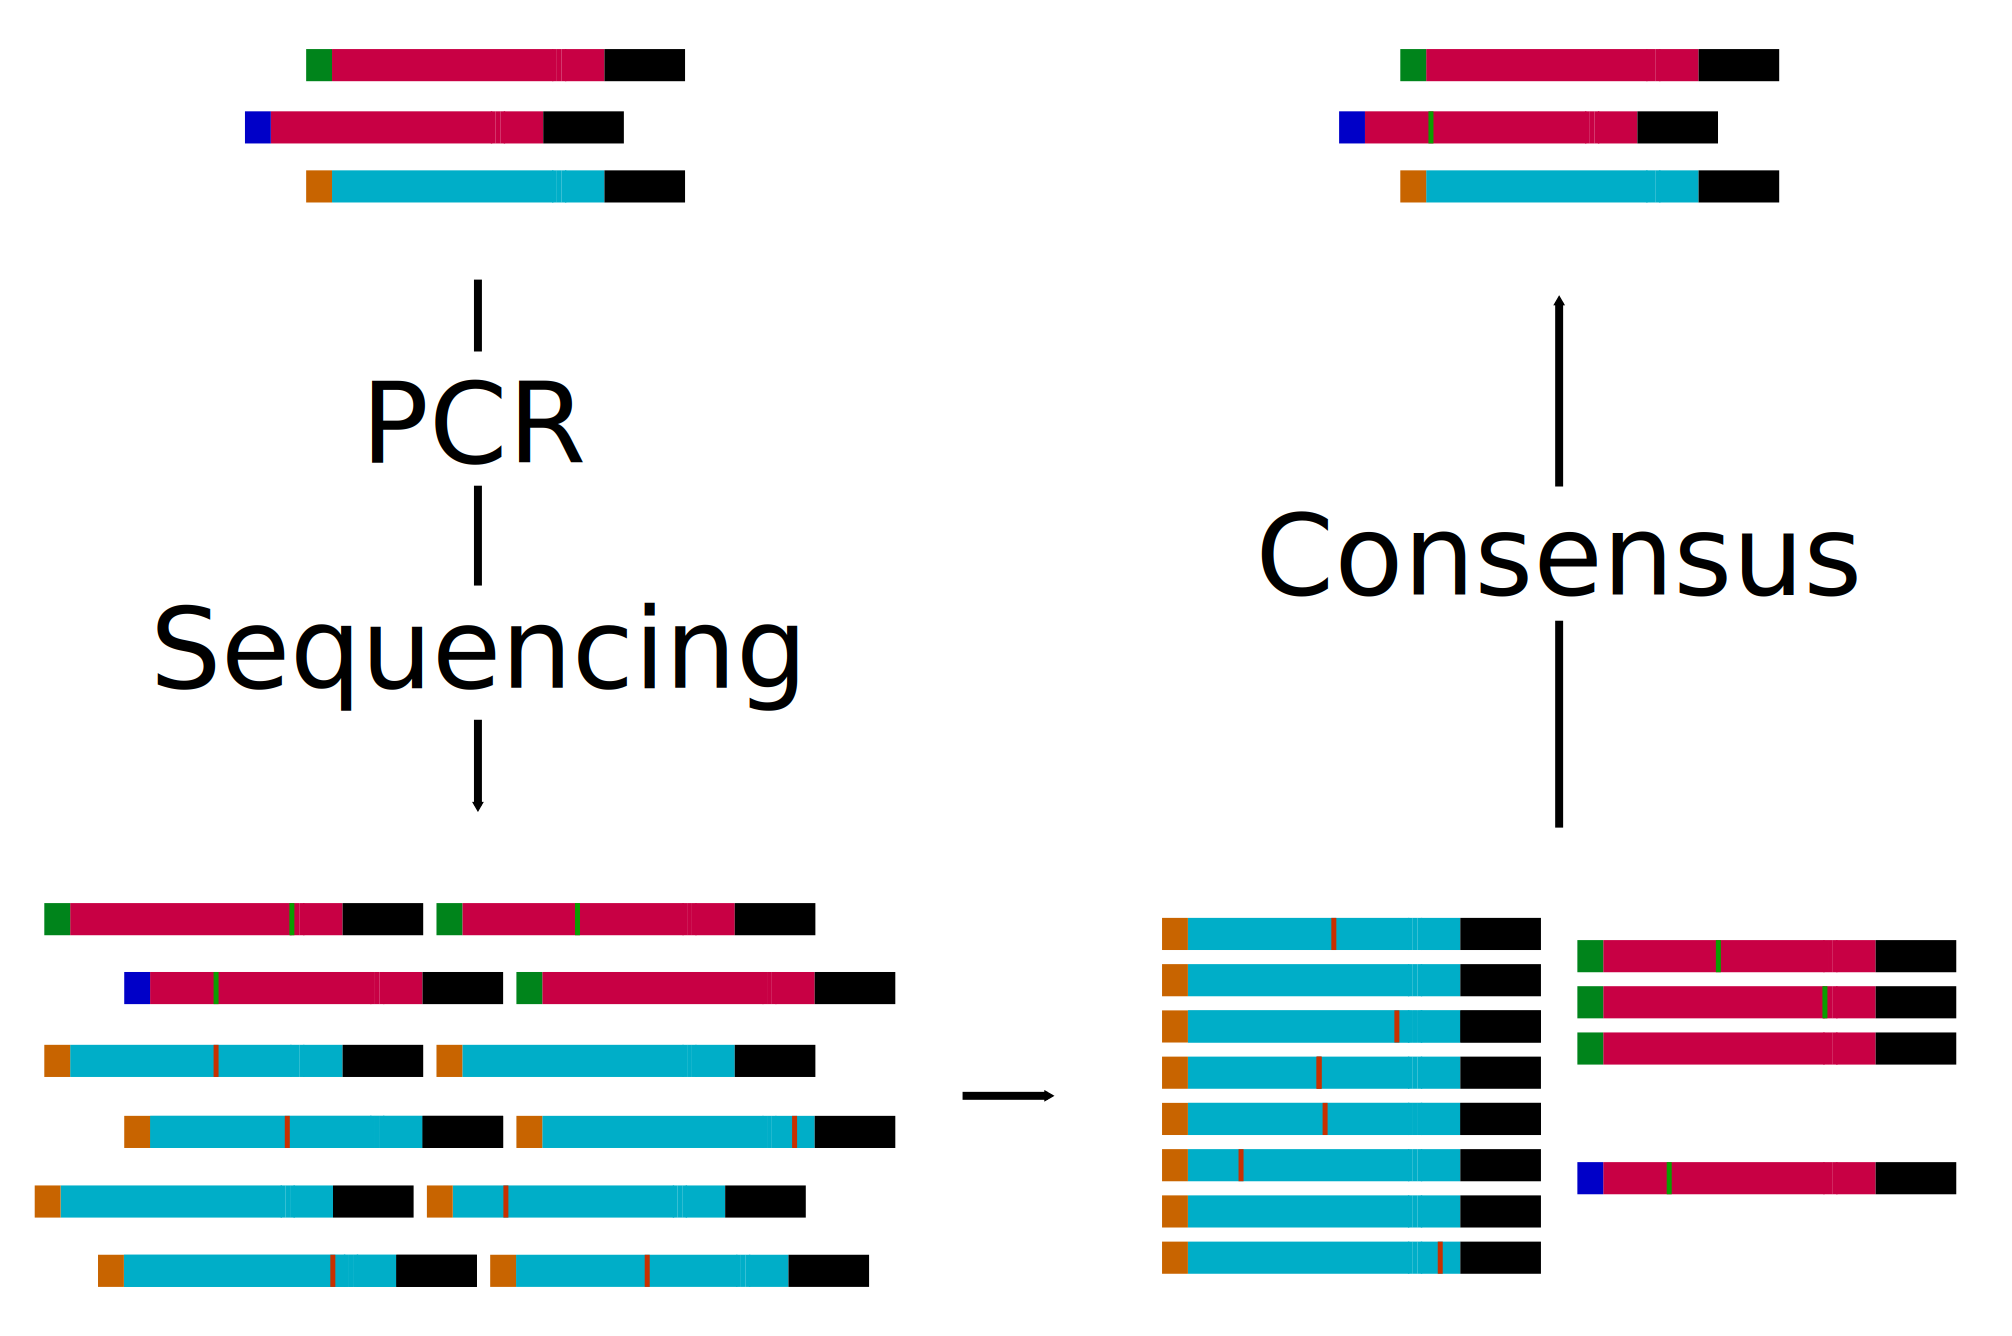
\includegraphics[width=0.7\textwidth]{output_files/figures/pdf/igseq-umi-consensus}
\Caption{Correcting errors and biases with unique molecular identifiers}{In this simplified schematic, three template RNA molecules representing two distinct sequences (red and blue rectangles) are tagged with unique molecular identifiers (UMIs, coloured left-hand ends) prior to PCR-based library preparation and sequencing. As a result of differential amplification bias between the sequences, the less-abundant input sequence gives rise to a larger number of sequencing reads; however, by aligning and collapsing matching UMI groups into consensus reads, the original proportions of the sample can be reconstructed. Consensus-read generation also enables the correction of various PCR and sequencing errors (thin red/green bars), the majority of which are present in only a minority of sequence copies within a UMI group; in this example, only the dark-blue UMI group, for which only a single sequencing read was obtained, cannot be effectively corrected in this way.}
\label{fig:umi-consensus-schema}
\end{figure}

\begin{figure}
\centering
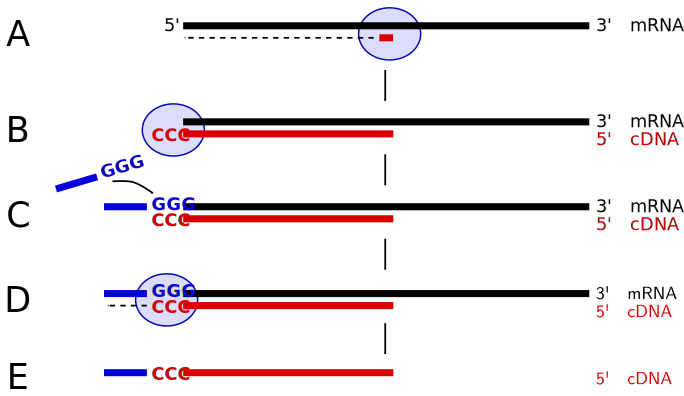
\includegraphics[width=0.7\textwidth]{output_files/figures/pdf/igseq-template-switch}
\vspace{0.5em}
\Caption{Addition of a known 5'-sequence to cDNA with template switching}{In this simplified schematic, an MMLV-derived reverse-transcriptase enzyme (blue oval) binds a primed RNA template and processes to the 5-prime end (A), where it deposits additional untemplated cytidine residues at the 3'-end of the cDNA (red bar) using its terminal-transferase activity (B). A template-switch adapter (TSA) with complementary terminal guanosine residues (blue bar) pairs with these terminal cytidines (C), creating a new double-stranded priming site to which the reverse-transcriptase enzyme can bind (D). Processing of the enzyme to the end of the TSA sequence produces a cDNA molecule with an additional, known 3' sequence (E).}
\label{fig:template-switch-schema}
\end{figure}

In the library-preparation protocol used for \Igseq in the turquoise killifish, therefore, reverse transcription is performed on total RNA using a gene-specific primer (GSP) homologous to the constant-region sequence of the isotype of interest and an MMLV-derived reverse-transcriptase enzyme optimised for its terminal-transferase activity (\Cref{sec:methods_molec_igseq_rt}). A template-switch adapter containing an invariant 5' primer sequence and random 3' UMI sequence (\Cref{fig:igseq-tsa-sequence}) is included in the reaction mixture and added to the cDNA sequence via template switching. In addition to enabling UMI-based clustering and correction as described above, this approach has the advantage of bypassing the variable region of the \igh{} transcript and thus avoiding the use of multiplexed V-segment primers, which may introduce additional biases through differential binding affinity between V-segments \parencite{rosati2017methods}.

\begin{figure}
\begin{center}
\LARGE
\textcolor{Fuchsia}{AAGCAGUGGTAUCAACGCAGAG}U\textcolor{ForestGreen}{NNNN}--\\--U\textcolor{ForestGreen}{NNNN}U\textcolor{ForestGreen}{NNNN}UCTT\textcolor{BurntOrange}{rGrGrGrG}
\end{center}
\Caption{The SmartNNNa template-switch adapter}{Annotated sequence of the SmartNNNa barcoded template-switch adapter (TSA) used in template-switch reverse transcription for \igseq library preparation \parencite{turchaninova2016igprep}. The 5'-terminal purple characters represent an invariant sequence used for primer-binding in downstream PCR steps, while the green N characters represent the random nucleotides constituting the unique molecular identifier (UMI), each of which could take any value from A, C, G or T. The U residues represent deoxyuridine, which is specifically digested after reverse transcription to remove residual TSA oligos from the reaction mixture (\Cref{sec:methods_molec_igseq_rt}). The orange, 3'-terminal rG characters indicate riboguanosine residues, which pair with terminal-transferase-added cytidine residues to enable template switching.}
\label{fig:igseq-tsa-sequence}
\end{figure}

\begin{figure}
\centering
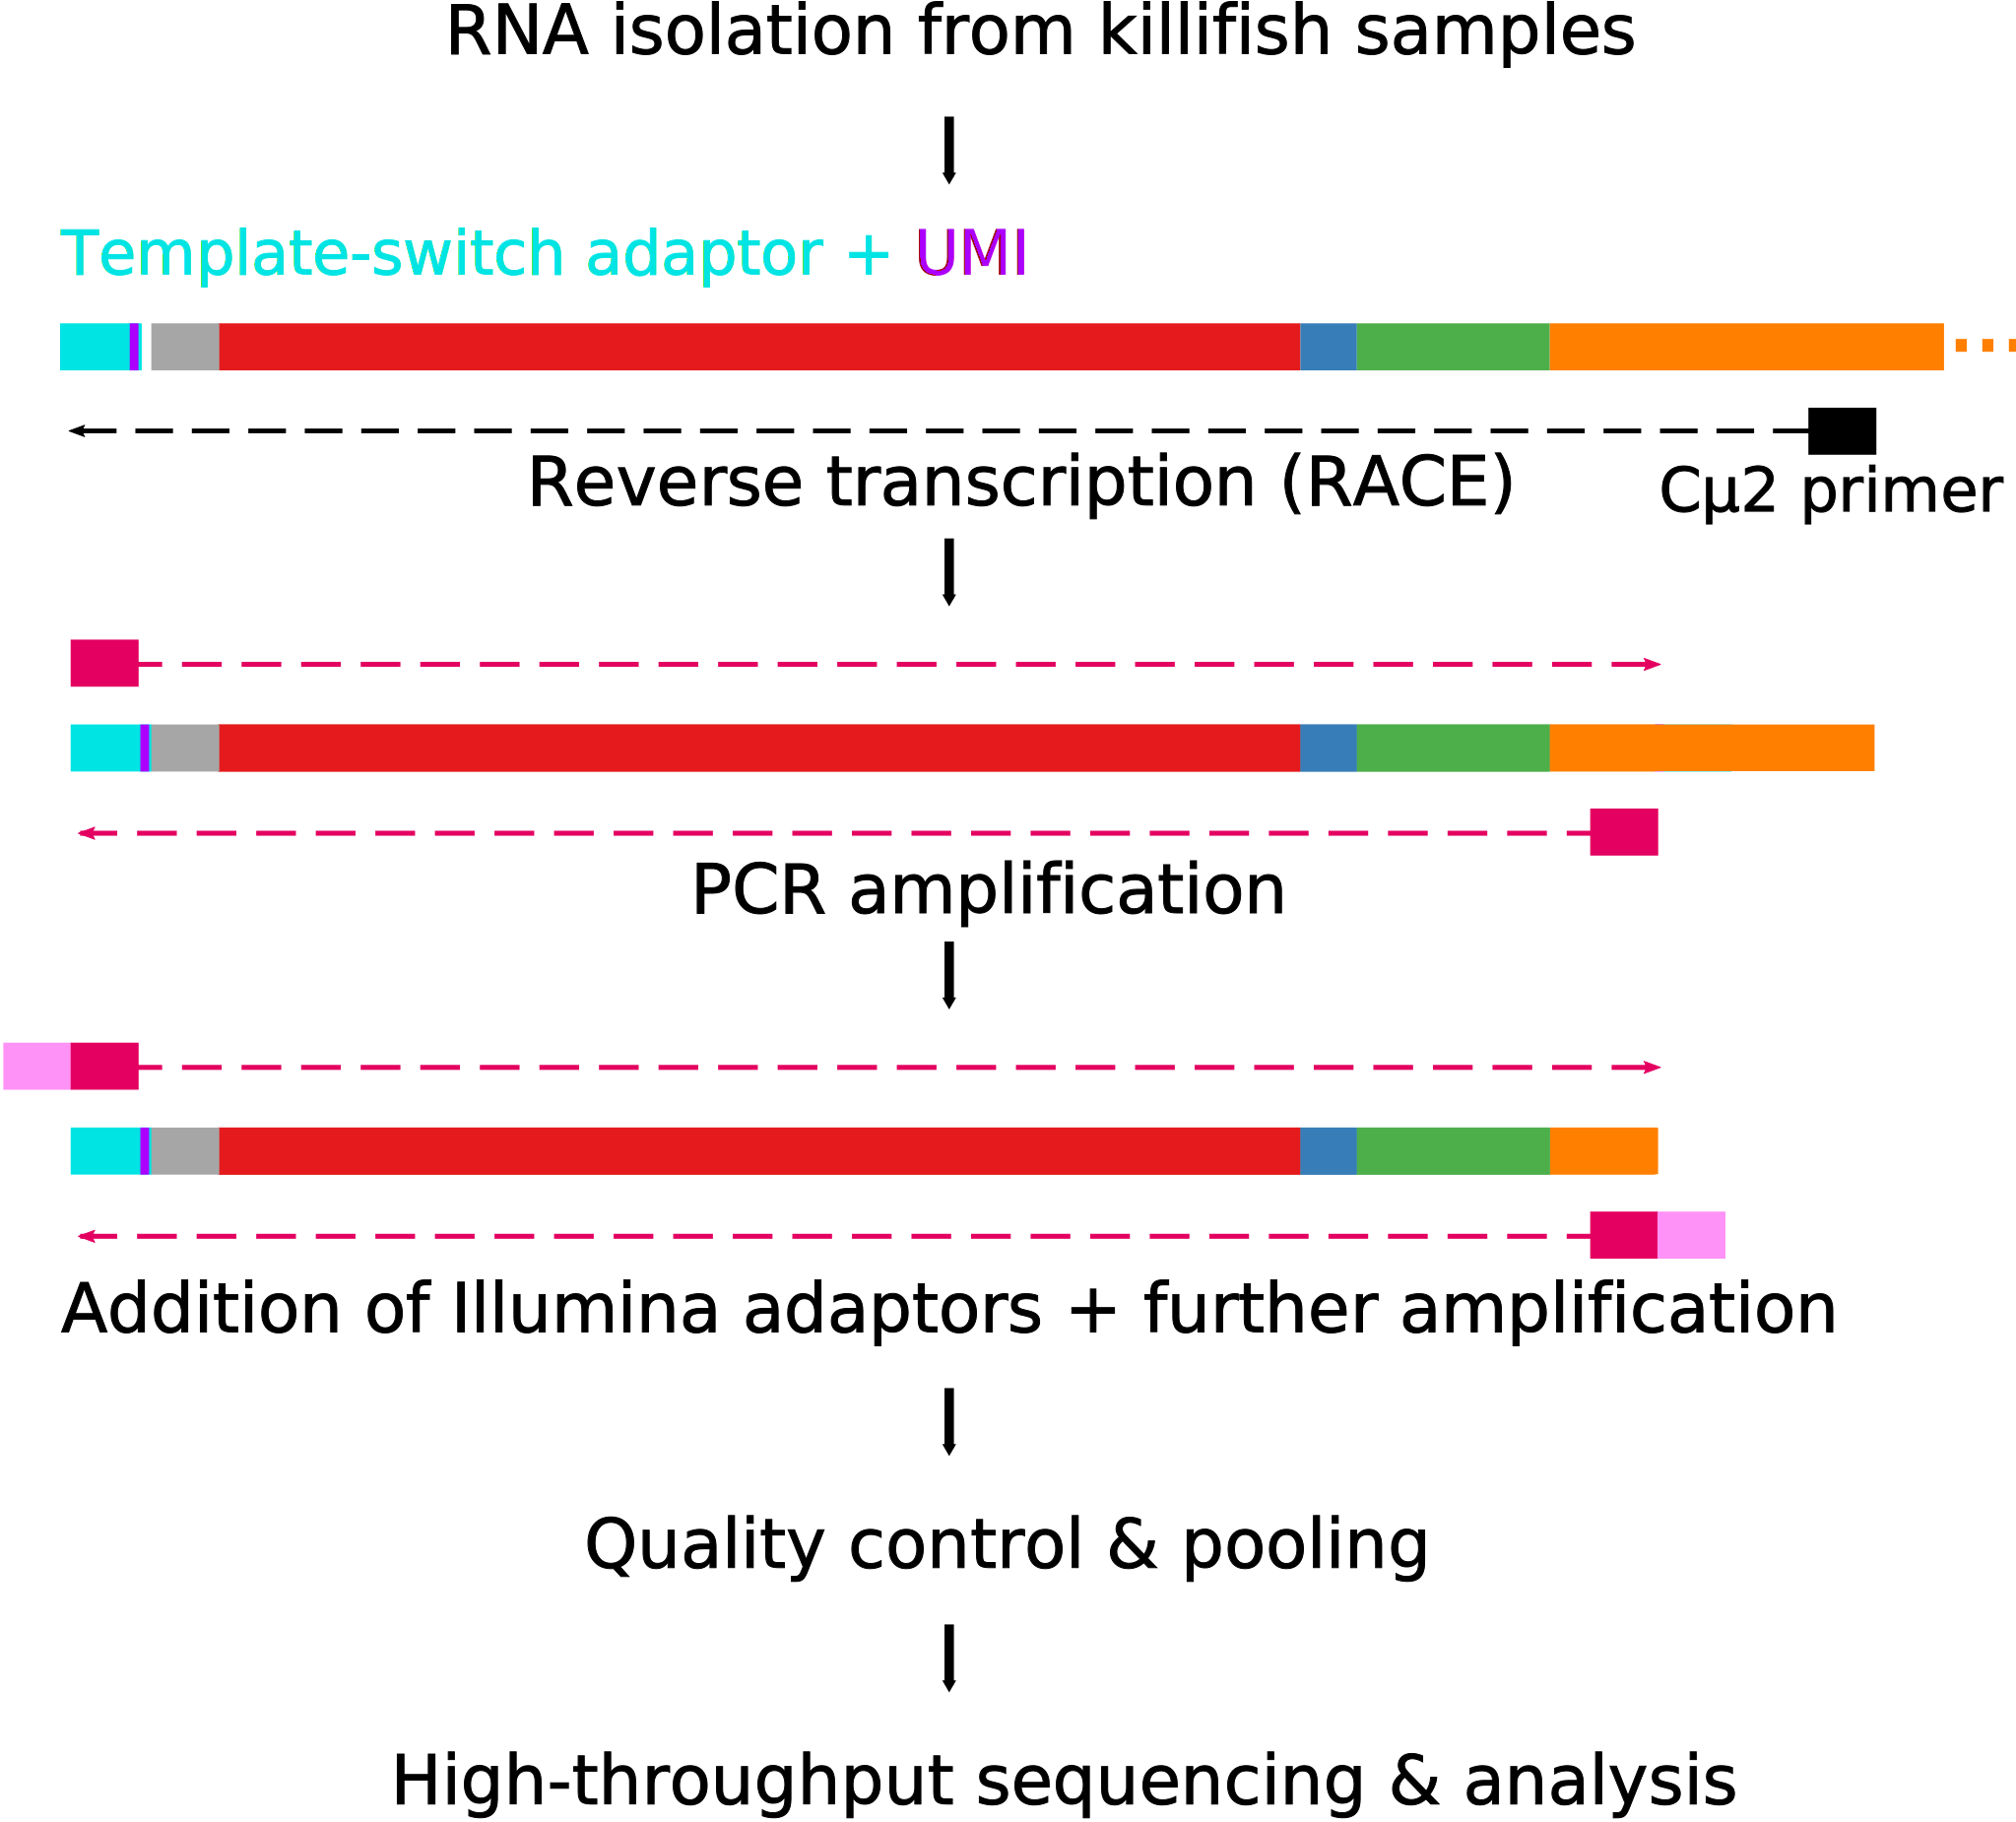
\includegraphics[width=0.7\textwidth]{output_files/figures/pdf/igseq-igrace-pipeline}
\Caption{Summary of the \igseq library-preparation protocol for turquoise-killifish samples}{Schematic summary of library-preparation protocol used to prepare immunoglobulin-sequencing libraries from turquoise-killifish samples. In order to capture all \igh{M} transcripts (both secreted and transmembrane), the reverse-transcription primer was homologous to the \cm{2} exon, while the PCR primers were homologous to \cm{1}. The third step (``Addition of Illumina adapters + further amplification'') represents two distinct rounds of PCR amplification and bead purification, for stepwise addition of Illumina TruSeq adapter sequences.}
\label{fig:igrace-pipeline}
\vspace{0.5em}
\end{figure}

Following reverse transcription, the reaction mixture is treated with uracil-DNA glycosylase (UDG) to specifically remove residual TSAs through digestion of deoxyuridine residues (which are absent in the template sequence). The library then undergoes three successive rounds of PCR amplification (\Cref{fig:igrace-pipeline}, \Cref{sec:methods_molec_igseq_pcr}), which respectively serve to amplify the reverse-transcribed cDNA sequence; amplify further while adding partial Illumina TruSeq adapter sequences; and add complete adapter sequences including library-specific P1 and P2 index sequences \parencite{vollmers2013consensus}. In the first two cases, the PCR primer sequences are homologous to the invariant part of the TSA sequence and the \cm{1} exon, respectively; as all known forms of \igh{} in turquoise killifish (\igh{M-TM}, \igh{M-S} and \igh{D-TM}) share this exon, the isotype- and isoform-specificity of the library prep can be altered simply by changing the position of the reverse-transcription GSP, with all other primer sequences left unchanged. In all experiments included in this chapter, a GSP on the \cm{2} exon was used, resulting in a library including \igh{M-TM} and \igh{M-S} sequences but excluding \igh{D}.

Libraries to be sequenced together are then pooled in equimolar ratio and the pooled sample undergoes size-selection to remove residual primer-dimers and other unwanted sequences (\Cref{sec:methods_molec_igseq_seq}). The complete library-preparation protocol reliably produces a single peak in the range of 650-\bp{680}, consistent with the known lengths of \vh, \dh and \jh gene segments in the \Nfu locus. Following size-selection and quality control, pooled libraries are sequenced on an Illumina MiSeq sequencing machine with 2$\times$\bp{300} reads (\Cref{sec:methods_molec_igseq_seq}); this longer read length is necessary to completely cover the variable region. To avoid problems associated with the low sequence complexity of single-amplicon sequencing libraries \parencite{illumina2017diversity}, a large proportion of PhiX spike-in (30\,\%) was used to increase the sequence complexity of the libraries.

\subsection{Sequence pre-processing with \program{pRESTO}}
\label{sec:igseq_protocol_preprocess}

\begin{figure}
\centering
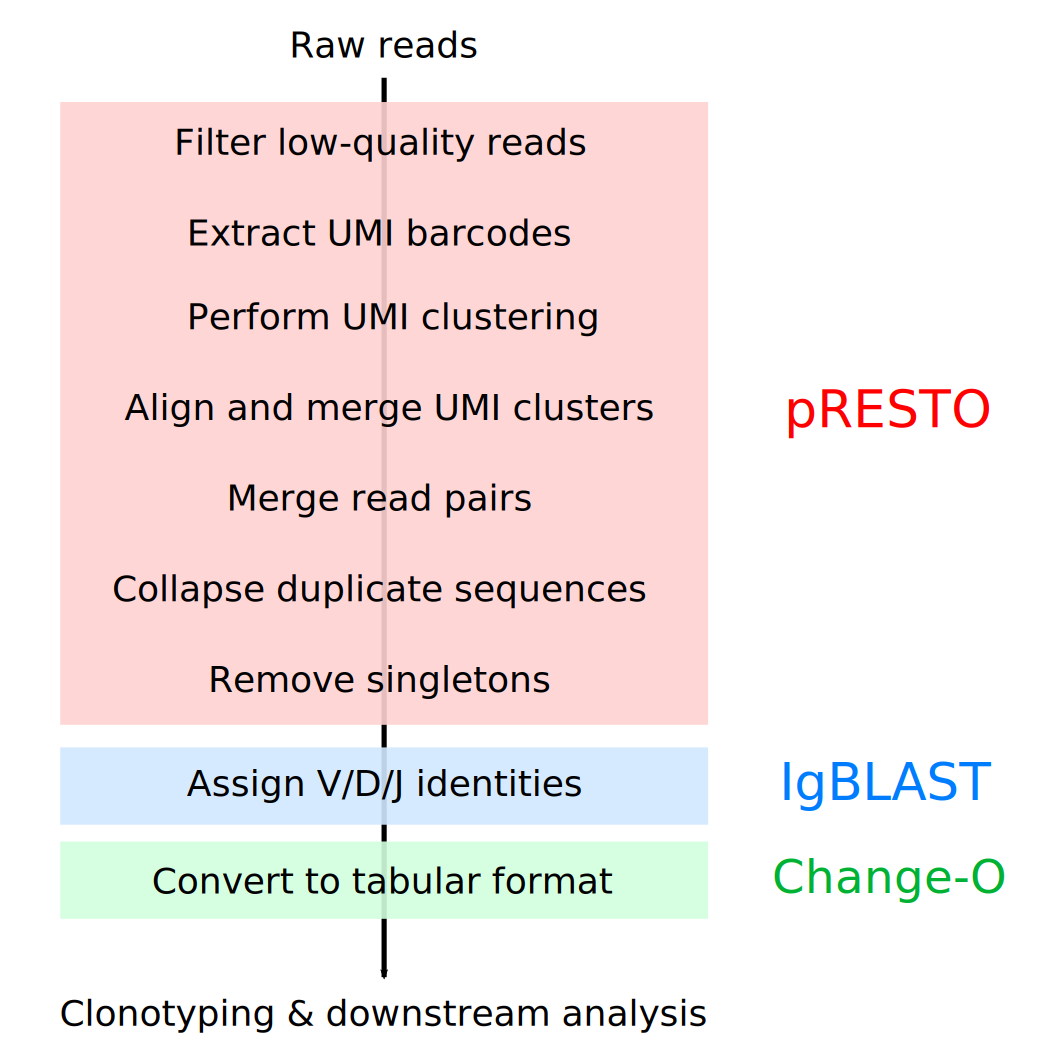
\includegraphics[width=0.6\textwidth]{output_files/figures/pdf/igseq-preprocessing}
\Caption{Summary of the \igseq pre-processing pipeline for turquoise-killifish data}{Schematic summary of post-sequencing analysis pipeline of killifish \igseq data, up to and including conversion from \format{FASTA} to \program{Change-O} tabular format. Clonotyping and additional downstream analysis methods are described in \Cref{sec:igseq_pilot,sec:methods_comp_igpreproc_clones,sec:methods_comp_igpreproc_clones}.}
\label{fig:igrace-preprocessing}
\vspace{0.5em}
\end{figure}

Raw \igseq data from the protocol described in \Cref{sec:igseq_protocol_library} takes the form of a large number of paired-end sequencing reads, each of which represents a single biased and error-prone observation from the set of input sequences in the original sample. To get from this fragmented and unreliable dataset to a set of complete, error-corrected and bias-adjusted \igh{} variable-region sequences, extensive pre-processing (\Cref{sec:methods_comp_igpreproc}) must be performed on the raw data. In this case, this pre-processing was largely carried out with \program{pRESTO} \parencite{vanderheiden2014presto}, part of the Immcantation suite of repertoire-sequencing analysis tools (\Cref{fig:igrace-preprocessing}).

To begin with, each read pair in the dataset is annotated with various information about the source individual (ID, strain, sex, age and weight at death, etc.) as well as information about its place in the replicate structure of the experiment (\Cref{sec:methods_comp_igpreproc_annot}). The sequences are then filtered to remove low-quality sequences (with a mean Phred score of less than 20 \parencite{ewing1998phred}). Invariant primer sequences are trimmed from the ends of the reads, and the UMI sequence of each forward read (containing the TSA sequence) is extracted into a sequence annotation and trimmed from the read sequence (\Cref{sec:methods_comp_igpreproc_mask}).

As discussed in \Cref{sec:igseq_protocol_library}, the use of UMI sequences enables biases and errors in library insert sequences to be corrected by taking the consensus sequence of all reads sharing a given UMI. However, PCR and sequencing errors can also affect the sequence of the UMI itself, in which case reads that in fact belong to a single group will be spuriously separated during pre-processing; this can result in spuriously low UMI group sizes, spuriously high numbers of unique sequences, and avoidable loss of sequencing data due to reads with erroneous barcodes being discarded (as low-quality, low-read-count unique sequences) at various points in the pre-processing pipeline \parencite{shlemov2017igrec}. In addition to these barcode \textit{errors}, barcode \textit{collisions} can occur, in which multiple distinct sequences are labelled with the same UMI sequence and spuriously grouped together during UMI grouping. This can lead to spuriously large UMI groups and spuriously low numbers of unique sequences, and in extreme cases can lead to the rejection and loss of entire UMI groups due to an insufficiently high level of internal sequence identity during consensus-read generation \parencite{shlemov2017igrec}.

In order to reduce the effect of such barcode errors and collisions on the pre-processing pipeline, primer-trimmed forward reads in this pipeline undergo clustering following extraction of UMI sequences (\Cref{sec:methods_comp_igpreproc_correct}). Firstly, reads are clustered by UMI sequence, and those with sufficiently similar UMIs are grouped together into a single cluster even if their UMIs differ slightly. Following this, the insert sequences (as opposed to UMI sequences) of the reads in each cluster are themselves clustered, and those with sufficiently different insert sequences are split apart into separate clusters. Following these clustering steps, each cluster consists of reads with highly similar barcode sequences as well as similar insert sequences; it is then these clusters, rather than the raw UMI sequences, on which consensus-read generation is performed.

Following cluster inference as described above, annotations (including barcode and cluster annotations) are copied from each TSA-bearing forward-read to its mate among the reverse reads. The forward and reverse reads were then separately grouped by cluster identity and collapsed into a consensus sequence (\Cref{sec:methods_comp_igpreproc_consensus}), based on the quality score of each aligned base call at each position \parencite{vanderheiden2014presto}. As most PCR and sequencing errors should be present in only a minority of the sequences descended from a given input sequence, this process effectively corrects these errors, while also removing the effect of biased amplification on observed sequence abundance. The more sequences present in a given cluster, the more effective is consensus-read generation at correcting these errors; as such, when sequencing \igseq libraries there is a trade-off inherent in the amount of oversequencing of the molecules in each library, with more reads per molecule improving error correction but reducing the amount of useful information gained per sequencing read \parencite{turchaninova2016igprep}.

Following consensus-read generation, pairs of forward and reverse consensus reads with matching cluster annotations are assembled into a single contiguous sequence, ideally covering the entire variable-region sequence of the template molecule (\Cref{sec:methods_comp_igpreproc_collapse}); forward or reverse consensus reads lacking a mate in the other read set are discarded. At this point in the pipeline, each entry is assumed to represent a distinct RNA template molecule in the original sample. Sequences with different cluster annotations but matching insert sequences are then collapsed together into a single sequence, which is annotated with the number of contributing consensus reads (\Cref{sec:methods_comp_igpreproc_collapse}); each sequence entry now represents a unique sequence in the dataset. Finally, unique sequences represented by only a single read pair (which could not be corrected by consensus-read generation and are therefore highly unreliable) are discarded.

At the end of the \program{pRESTO} pre-processing pipeline, the raw data has been processed into a set of complete variable-region sequences, each of which is annotated with the number of contributing reads and the number of distinct instances of that sequence found in the dataset. These sequences are then assigned V/D/J-identities through alignment to reference databases with \program{IgBLAST} (\Cref{sec:methods_comp_igpreproc_igblast}) \parencite{ye2013igblast}. Finally, the sequences and their metadata, including annotations and V/D/J-identities, are converted by \program{Change-O} (another program from the Immcantation suite) \parencite{gupta2015changeo} into tabular format for efficient downstream processing and analysis (\Cref{fig:igrace-preprocessing}).

\FloatBarrier
\clearpage

\section{Establishing \igseq in the turquoise killifish: pilot study}
\label{sec:igseq_pilot}

In order to refine and functionally validate the library-preparation protocol and processing pipeline described in \Cref{sec:igseq_protocol}, as well as assess the state of the turquoise-killifish antibody repertoire in mature adults, I selected a group of four killifish from the second, eight-week-old sample group (specifically, fish 2-03, 2-04, 2-05 and 2-06 from \Cref{tab:igseq-cohorts-fish}) for a pilot study. In this experiment, total RNA was isolated twice independently from each fish, and independent library preps were performed once on the first RNA isolate and twice on the second, for a total of three replicates per individual (\Cref{fig:igseq-pilot-design}). These twelve replicates were sequenced together in a single MiSeq run, yielding a total of \embed{output_files/txt/igseq-pilot-nreads-raw-total.txt} million read pairs (\embed{output_files/txt/igseq-pilot-nreads-raw-replicate-min.txt} to \embed{output_files/txt/igseq-pilot-nreads-raw-replicate-max.txt} million pairs per replicate, \embed{output_files/txt/igseq-pilot-nreads-raw-individual-min.txt} to \embed{output_files/txt/igseq-pilot-nreads-raw-individual-max.txt} million pairs per individual). These data were then used to develop the downstream analysis pipeline for killifish immunoglobulin-sequencing data, validate the performance and replicability of the protocol, and investigate the state of the antibody repertoire in mature adult killifish.

\begin{figure}
\centering
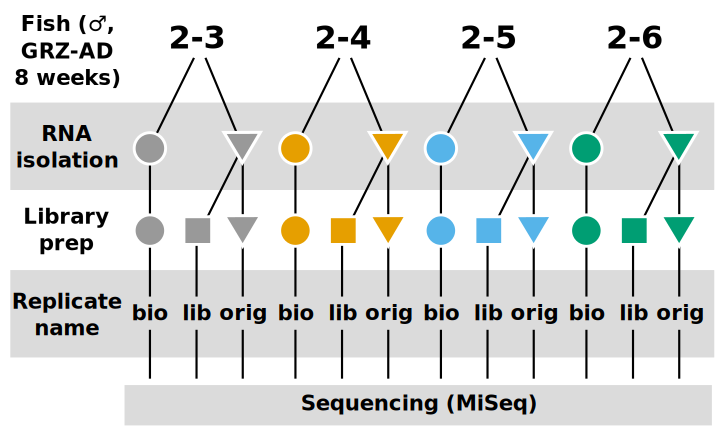
\includegraphics[width = 0.9\textwidth]{output_files/figures/pdf/igseq-pilot-design}
\caption[Experimental design of killifish \igseq pilot study]{\textbf{Experimental design of killifish \igseq pilot study}, showing relationship between replicates for each individual. Colour denotes individual of origin, while shape denotes replicate type.}
\label{fig:igseq-pilot-design}
\end{figure}

\subsection{Read survival and composition}
\label{sec:igseq_pilot_composition}

\Cref{fig:igseq-pilot-read-survival-init} shows the absolute and relative read survival for each of the twelve replicates throughout the pre-processing pipeline, up to and including VDJ assignment and Change-O table construction. The twelve replicates show relatively consistent behaviour, with \embed{output_files/txt/igseq-pilot-read-survival-init-min.txt}\,\% to \embed{output_files/txt/igseq-pilot-read-survival-init-max.txt}\,\% of reads surviving the entire process. Of those that do not, the biggest losses typically occur during quality filtering and removal of singleton sequences, with most other steps giving rise to relatively little sequence loss (\Cref{fig:igseq-pilot-read-survival-init-b}).

\begin{figure}
\centering
\includegraphics[width = 0.9\textwidth]{output_files/figures/pdf/igseq-pilot-read-survival-init}
\begin{subfigure}{0em}
\phantomsubcaption{}
\label{fig:igseq-pilot-read-survival-init-a}
\end{subfigure}
\begin{subfigure}{0em}
\phantomsubcaption{}
\label{fig:igseq-pilot-read-survival-init-b}
\end{subfigure}
\Caption{Read survival during initial pre-processing of the \igseq pilot dataset}{Line graphs of absolute (A) and relative (B) read survival during pre-processing of the \igseq pilot dataset, up to VDJ assignment and Change-O table construction.}
\label{fig:igseq-pilot-read-survival-init}
\end{figure}

In total, the pre-processed sequence repertoires of the pilot replicates contain between \embed{output_files/txt/igseq-pilot-nseq-init-replicate-min.txt} and \embed{output_files/txt/igseq-pilot-nseq-init-replicate-max.txt} unique sequences per replicate, corresponding to between \embed{output_files/txt/igseq-pilot-nseq-init-individual-min.txt} and \embed{output_files/txt/igseq-pilot-nseq-init-individual-max.txt} unique sequences per individual killifish and \embed{output_files/txt/igseq-pilot-nseq-init-total.txt} unique sequences in total. Of these, \embed{output_files/txt/igseq-pilot-nseq-init-pc-functional.txt}\,\% of sequences (corresponding to \embed{output_files/txt/igseq-pilot-nreads-init-pc-functional.txt}\,\% of surviving sequencing reads) are annotated by \program{Change-O} as functional, meaning they have successfully been assigned V- and J-identities, their V- and J-sequences are in-frame, and they do not contain any stop codons (\Cref{fig:igseq-pilot-functional-prop-a}). A further \embed{output_files/txt/igseq-pilot-nseq-init-pc-noj.txt}\,\% of sequences (corresponding to \embed{output_files/txt/igseq-pilot-nreads-init-pc-noj.txt}\,\% of surviving reads) failed to be assigned even an uncertain J-identity, meaning that no \jh sequence in the reference database aligned to the insert sequence; the remaining \embed{output_files/txt/igseq-pilot-nseq-init-pc-other.txt}\,\% of sequences (corresponding to \embed{output_files/txt/igseq-pilot-nreads-init-pc-other.txt}\,\% of surviving reads) have a J-assignment but are rendered nonfunctional by an internal stop codon and/or a frameshift between their V- and J-sequences (\Cref{fig:igseq-pilot-functional-prop-a}), arising during primary diversification (\Cref{sec:intro_immunity_primary}) or possibly SHM.

\begin{figure}
\centering
\includegraphics[width = 0.9\textwidth]{output_files/figures/pdf/igseq-pilot-functional-prop}
\begin{subfigure}{0em}
\phantomsubcaption{}
\label{fig:igseq-pilot-functional-prop-a}
\end{subfigure}
\begin{subfigure}{0em}
\phantomsubcaption{}
\label{fig:igseq-pilot-functional-prop-b}
\end{subfigure}
\Caption{Functional composition and V-score filtering in the \igseq pilot dataset}{Proportion of input reads, UMI groups and unique sequences in the \igseq pilot dataset belonging to different (non)functional categories, before (A) and after (B) filtering on V-alignment score.}
\label{fig:igseq-pilot-functional-prop}
\end{figure}

As genuinely rearranged but nonfunctional sequences would be expected to have undergone V(D)J recombination and so have a complete J-sequence, the lack of assigned J-identities for a significant minority of sequences suggests that this subset of sequences may be artefactual, erroneous or otherwise malformed. Supporting this assumption, sequences without J-assignments overwhelmingly have very low V-alignment scores reported by \program{IgBLAST}, with an average score of \embed{output_files/txt/igseq-pilot-vscore-mean-noj.txt} $\pm$ \embed{output_files/txt/igseq-pilot-vscore-sd-noj.txt} (mean $\pm$ standard deviation), compared to \embed{output_files/txt/igseq-pilot-vscore-mean-other.txt} $\pm$ \embed{output_files/txt/igseq-pilot-vscore-sd-other.txt} for other nonfunctional sequences and \embed{output_files/txt/igseq-pilot-vscore-mean-functional.txt} $\pm$ \embed{output_files/txt/igseq-pilot-vscore-sd-functional.txt} for functional sequences (\Cref{fig:igseq-pilot-functional-vscores}). A simple V-score cut-off of 100, therefore, effectively removes the vast majority of these low-quality sequences, while leaving the population of functional sequences intact (\Cref{fig:igseq-pilot-functional-prop-b}).

\begin{figure}
\centering
\includegraphics[width = 0.9\textwidth]{output_files/figures/pdf/igseq-pilot-functional-vscores}
\Caption{V-score distributions of functional and nonfunctional sequences}{Kernel density plots of distributions of V-alignment scores among unique sequences in the \igseq pilot dataset. Vertical axes are not to scale between sequence categories.}
\label{fig:igseq-pilot-functional-vscores}
\end{figure}

In total, \embed{output_files/txt/igseq-pilot-nseq-init-dropped-vscore.txt} unique sequences, corresponding to \embed{output_files/txt/igseq-ageing-rel-loss-total.txt}\,\% of input reads, were removed in this way. As a result, including this final filtering step, between \embed{output_files/txt/igseq-pilot-read-survival-all-min.txt}\,\% and \embed{output_files/txt/igseq-pilot-read-survival-all-max.txt}\,\% of reads per input library survived up to this point in the pipeline (\Cref{fig:igseq-pilot-read-survival-all}), a good range suggesting both that the library-preparation protocol successfully captured antibody-repertoire sequencing data from turquoise killifish for the first time, and that the subsequent computational pipeline was able to completely and successfully process the majority of the resulting data. Of the remaining \embed{output_files/txt/igseq-pilot-nseq-init-kept-vscore.txt} unique sequences present in the dataset, \embed{output_files/txt/igseq-pilot-nseq-init-functional-filtered.txt} (\embed{output_files/txt/igseq-pilot-nseq-init-pc-functional-filtered.txt}\,\%) are functional, \embed{output_files/txt/igseq-pilot-nseq-init-other-filtered.txt} (\embed{output_files/txt/igseq-pilot-nseq-init-pc-other-filtered.txt}\,\%) are rendered nonfunctional by a stop codon or frameshift, and only \embed{output_files/txt/igseq-pilot-nseq-init-noj-filtered.txt} (\embed{output_files/txt/igseq-pilot-nseq-init-pc-noj-filtered.txt}\,\%) could not be assigned a J-identity (\Cref{fig:igseq-pilot-functional-prop-b}). These results confirm that the data from this first \igseq experiment in the turquoise killifish are of sufficient quality to proceed to clonotyping and analysis of repertoire diversity.

\subsection{Clonotyping and clonal repertoire diversity}
\label{sec:igseq_pilot_clones}

Following assignment of VDJ identities and quality filtering, sequences in an antibody repertoire can be assigned to clones: groups of B-cells descended from a single \naive B-cell ancestor, and therefore sharing a single VDJ-recombination event. Sequences in the same clone are said to share a \textit{clonotype}. In \program{Change-O}, clonotyping is performed by dividing sequences into groups sharing a consistent V-assignment, J-assignment and CDR3 length, then performing single-linkage clustering on each group of sequences based on Hamming distances between CDR3 sequences \parencite{gupta2017hierarchical}. To identify a distance threshold for cutting the cluster dendrogram into clones, each unique sequence in the repertoire is assigned a nearest-neighbour distance based on the length-normalised Hamming distance to the most similar sequence in the repertoire. The resulting nearest-neighbour distribution is typically bimodal, with the lower peak (representing more-similar sequences) indicating members of the same clonotype and the higher peak (representing less-similar sequences) indicating members of different clones; by fitting a pair of gamma or normal distributions to these two peaks, a distance threshold for clonotype membership can be determined according to the desired levels of sensitivity and specificity \parencite{nouri2018threshold} (\Cref{sec:methods_comp_igpreproc_clones}). By cutting the cluster dendrogram at this threshold, each group of repertoire sequences can be separated into some number of distinct clones, each of which is assumed to share a unique \naive B-cell ancestor.

One disadvantage of single-linkage clustering in this context is that non-informative \sequence{N} positions can result in artifactual links between unrelated sequences. As such, sequences with a large number of junctional \sequence{N} positions can significantly disrupt the clonotyping process. On the other hand, as over \embed{output_files/txt/igseq-pilot-filtered-nn-any.txt}\,\% of unique sequences in the pilot dataset contain at least one such junctional \sequence{N} position, excluding them all would represent a significant loss of data. In order to minimise the number of discarded sequences while also minimising the disrupting effects of sequences with junctional \sequence{N}s, sequences with exactly one junctional \sequence{N} position (comprising \embed{output_files/txt/igseq-pilot-filtered-1n-total.txt}\,\% of total sequences and \embed{output_files/txt/igseq-pilot-filtered-1n-withn.txt}\,\% of sequences with at least one junctional \sequence{N}; \Cref{tab:igseq-pilot-filtered-nn}) were included in the clonotyping process for the pilot dataset, while those with two or more junctional \sequence{N} positions were excluded. This procedure successfully assigned clonal identities to \embed{output_files/txt/igseq-pilot-nseq-assigned-clones.txt}\,\% of unique sequences in the V-score-filtered dataset, with fewer than \embed{output_files/txt/igseq-pilot-nseq-lost-clonotyping.txt} sequences (corresponding to \embed{output_files/txt/igseq-pilot-pc-reads-lost-clonotyping.txt}\,\% of input reads) lost during the clonotyping phase of the pipeline.

\begin{table}
\caption{Distribution of junctional \sequence{N} positions in the V-score-filtered pilot dataset}
\label{tab:igseq-pilot-filtered-nn}
% latex table generated in R 3.5.2 by xtable 1.8-3 package
% Wed Apr  3 14:27:33 2019
\begin{tabular}{lrrr}
  \toprule \# junctional Ns & \# unique sequences & \% of all sequences & \% of sequences with $>$0 junctional Ns \\ 
  \midrule 0 & 49134 & 88.924 & 0.00 \\ 
  1 & 3388 & 6.132 & 67.94 \\ 
  2 & 961 & 1.739 & 19.27 \\ 
  3 & 324 & 0.586 & 6.50 \\ 
  4 & 125 & 0.226 & 2.51 \\ 
  5 & 93 & 0.168 & 1.86 \\ 
  $>$5 & 96 & 0.174 & 1.93 \\ 
   \bottomrule \end{tabular}

\end{table}

In total, \embed{output_files/txt/igseq-pilot-nclones-individual-min.txt} to \embed{output_files/txt/igseq-pilot-nclones-individual-max.txt} clones were identified per individual fish in the pilot dataset. As expected, the clone-size distribution is overwhelmingly dominated by small clones (\Cref{fig:igseq-pilot-clone-sizes-sizes}): across all individuals, \embed{output_files/txt/igseq-pilot-nclones-pc-1count.txt}\,\% of clones are observed as just a single unique sequence across all replicates, while \embed{output_files/txt/igseq-pilot-nclones-pc-small.txt}\,\% contain fewer than five unique sequences. As a result, the great majority of clones (\embed{output_files/txt/igseq-pilot-nclones-pc-1rep.txt}\,\%) are observed in only a single replicate per individual, with \embed{output_files/txt/igseq-pilot-nclones-pc-2rep.txt}\,\% present in two replicates and only \embed{output_files/txt/igseq-pilot-nclones-pc-1rep.txt}\,\% shared across all three. Unsurprisingly, however, larger clones are much more likely to be shared across multiple replicates (\Cref{fig:igseq-pilot-clone-sizes-reps}), consistent with a model in which a very large number of small clones are sampled only rarely while a much smaller number of large clones is sampled much more often \parencite{mora2016diversity}. Overall, the level of agreement between the replicates is high (\Cref{fig:igseq-pilot-clone-sizes-cor}), with an average inter-replicate correlation in clone size of $r=\embed{output_files/txt/igseq-pilot-clones-interrep-cor-avg.txt}$, indicating that, despite the problem of undersampling many very small clones, the clonal composition of the killifish can be captured reproducibly by \Igseq.

\begin{figure}
\centering
\includegraphics[width = 0.9\textwidth]{output_files/figures/pdf/igseq-pilot-clone-sizes}
\begin{subfigure}{0em}
\phantomsubcaption{}
\label{fig:igseq-pilot-clone-sizes-sizes}
\end{subfigure}
\begin{subfigure}{0em}
\phantomsubcaption{}
\label{fig:igseq-pilot-clone-sizes-reps}
\end{subfigure}
\Caption{Clone size and cross-replicate reproducibility in the \igseq pilot dataset}{(A) Proportion of clones of different sizes for each individual in the pilot dataset, measured in unique sequences per clone. (B) LOESS-smoothed curves \parencite{cleveland1991loess} showing proportion of clones of each size found across one, two or all three replicates of the appropriate individual.}
\label{fig:igseq-pilot-clone-sizes}
\end{figure}

\begin{figure}
\centering
\includegraphics[width = 0.75\textwidth]{output_files/figures/pdf/igseq-pilot-clone-sizes-cor}
\begin{subfigure}{0em}
\phantomsubcaption{}
\label{fig:igseq-pilot-clone-sizes-cor-boxplots}
\end{subfigure}
\begin{subfigure}{0em}
\phantomsubcaption{}
\label{fig:igseq-pilot-clone-sizes-cor-scatter}
\end{subfigure}
\Caption{Clone-size correlation between pilot replicates}{(A) Boxplots showing distribution of Pearson product-moment correlation coefficients of clone sizes for each pair of replicates, as measured by the number of unique sequences per clone in each replicate. (B) Scatter plots comparing clone sizes across biological replicates for each individual in the pilot dataset. In both subfigures, clones absent in a given replicate were given a size of zero.}
\label{fig:igseq-pilot-clone-sizes-cor}
\end{figure}

One of the most strikingly reproducible findings of immune-repertoire-sequencing studies has been the approximately power-law distribution of the clonal repertoire, a phenomenon observed in both antibody and TCR repertoires across multiple different species \parencite{desponds2016fluctuating,mora2016diversity}. More precisely, the frequency of the $k$th largest clone in a repertoire dataset containing $N$ total clones can often be roughly predicted by a Zipf distribution \parencite{mora2010mentropy} of the form:

\begin{equation}
f(k | N, s) = \frac{k^{-s}}{H_{N,s}}
\end{equation}

\noindent for some exponent parameter $s > 0$, where $H_{N,s}$ is the $N$th generalised harmonic number of order $s$ (\Cref{sec:methods_comp_igdownstream_zipf}). This power-law distribution of clone sizes is inconsistent with clonal expansion under neutral selection and instead suggests that clone sizes evolve within a complex and fluctuating fitness landscape \parencite{desponds2016fluctuating}. Before going on with more detailed investigation of the diversity structure of turquoise killifish antibody repertoires, it would be interesting to test whether the phenomenon of roughly Zipf-distributed clonal frequencies persists in this species as well.

\Cref{fig:igseq-pilot-clones-zipf-lines} shows the rank/frequency distributions of the clonal repertoires of the four individuals from the pilot dataset. From roughly the tenth-largest clone onwards, these distributions appear approximately linear on a log-log plot and can be reasonably approximated by a power-law distribution; however, the largest clones in each repertoire clearly deviate from this pattern, and are much larger than would be predicted by a power-law approximation. In order to fit power-law curves to these distributions, I performed simple maximum-likelihood estimation of the Zipf exponent for each individual repertoire in \program{R} (\Cref{sec:methods_comp_igdownstream_zipf}). When the five largest clones in each repertoire were excluded from the calculation, the resulting Zipf distributions (\Cref{fig:igseq-pilot-clones-zipf-fit}) provided a good approximation of the remaining points and were highly consistent across individuals, with exponents ranging from \embed{output_files/txt/igseq-pilot-clone-zipf-exp-min.txt} to \embed{output_files/txt/igseq-pilot-clone-zipf-exp-max.txt}. Conversely, when the largest clones are included, the resulting Zipf approximations follow the line of the remaining clones much less accurately in several individuals, and their exponents range more widely from \embed{output_files/txt/igseq-pilot-clone-zipf-exp-null-min.txt} to \embed{output_files/txt/igseq-pilot-clone-zipf-exp-null-max.txt}. Hence, while the bulk of the clonal repertoire in turquoise killifish corresponds to the expected power-law behaviour seen in other species, the largest clones, for unknown reasons, consistently deviate strongly from this pattern.

\begin{figure}
\centering
\includegraphics[width=0.8\textwidth]{output_files/figures/pdf/igseq-pilot-clone-zipf-lines}
\Caption{Rank/frequency distributions of pilot clonal repertoires}{Log-log line plots of rank/frequency distributions of the individual clonal repertoires in the \igseq pilot dataset, showing the roughly linear (i.e. power-law-distributed) distribution of smaller clones (roughly rank 10 onwards) and the clear deviation from this distribution in the largest clones.}
\label{fig:igseq-pilot-clones-zipf-lines}
\end{figure}

\begin{figure}
\centering
\includegraphics[width=0.7\textwidth]{output_files/figures/pdf/igseq-pilot-clone-zipf-grad}
\begin{subfigure}{0em}
\phantomsubcaption{}
\label{fig:igseq-pilot-clones-zipf-fit}
\end{subfigure}
\begin{subfigure}{0em}
\phantomsubcaption{}
\label{fig:igseq-pilot-clones-zipf-fit-null}
\end{subfigure}
\Caption{Best-fit Zipf distributions of pilot clonal repertoires}{Log-log scatter plots of the rank/frequency distributions for each clonal repertoire in the pilot dataset, overlaid with a maximum-likelihood estimate of the underlying Zipf distribution computed (A) with the five largest clones excluded or (B) with all clones included. In (A), the clones excluded from the Zipf estimation are plotted as crosses.}
\label{fig:igseq-pilot-clones-zipf-fit-grid}
\end{figure}

In addition to the exponent of the best-fit Zipf distribution, another quick and simple way to measure the extent to which a clonal repertoire is dominated by the largest clones is to measure the P20, the proportion of all unique sequences in the repertoire belonging to the 20 largest clones; in humans, for example, the P20 is typically a few percent in healthy individuals, but can reach up to 90\,\% in patients with B-cell malignancies \parencite{rosenfeld2018clonesize}. In the killifish pilot dataset, the P20 of the clonal repertoires ranges from \embed{output_files/txt/igseq-pilot-clone-zipf-p20-obs-min.txt}\,\% to \embed{output_files/txt/igseq-pilot-clone-zipf-p20-obs-max.txt}\,\% (\Cref{fig:igseq-pilot-clones-zipf-p20}), much higher than that observed in healthy humans. These high P20 values are primarily due to the highly expanded state of the largest few clones in each repertoire; when the expected clonal frequencies from the Zipf distributions fitted in \Cref{fig:igseq-pilot-clones-zipf-fit} are used instead of the actual values, the P20 values fall to between \embed{output_files/txt/igseq-pilot-clone-zipf-p20-exp-min.txt}\,\% and \embed{output_files/txt/igseq-pilot-clone-zipf-p20-exp-max.txt}\,\% (\Cref{fig:igseq-pilot-clones-zipf-p20}).

\begin{figure}
\centering
\includegraphics[width=0.8\textwidth]{output_files/figures/pdf/igseq-pilot-clone-p20}
\Caption{Clonal P20 values in \Nfu pilot repertoires}{(A) Boxplots of observed and expected (from the Zipf distributions fitted in \Cref{fig:igseq-pilot-clones-zipf-fit}) P20 distributions of the clonal repertoires from the \igseq pilot dataset. Pairwise $p$-value computed using nonparametric Mann-Whitney $U$ test ($*: 0.01 < p \leq 0.05;~**: 0.001 < p \leq 0.01;~***: p \leq 0.001$) . (B) Scatter plot comparing observed vs expected P20 for each individual, annotated with the correlation ($r$) between the two sets of P20 values.}
\label{fig:igseq-pilot-clones-zipf-p20}
\end{figure}

In addition to investigating the P20, Rosenfeld \textit{et al.} \parencite{rosenfeld2018clonesize} recommend evaluating clonal expansions in antibody repertoires on the basis of both the relative clonal frequency of the largest clones in the repertoire and the extent to which each such clone is larger than the next-largest clone, with recommended cutoffs for human data of 5\,\% for the former and threefold for the latter. In the pilot killifish dataset, clones exceeding 5\,\% of unique sequences in the repertoire occur in three out of four individuals (2-03, 2-04 and 2-06), while clones exceeding the size of the next-largest clone by at least threefold occur in a different three individuals (2-03, 2-05 and 2-06). However, only one individual, 2-04, exhibits a potentially medically-relevant clonal expansion by the standards of Rosenfeld \textit{et al.}; this clone (2-04\_8143) occupies 6.8\,\% of the repertoire and is roughly 3.1-fold larger than the next-largest clone, and is identified reproducibly as a clonal expansion in both the pooled dataset (\Cref{fig:igseq-pilot-clones-expansions}) and each of the separate replicates (\Cref{fig:igseq-pilot-clones-expansions-rep}) from individual 3-04. These results could be taken as demonstrating that potentially medically-relevant clonal expansions are present, albeit not common, in middle-aged adult male turquoise killifish; however, without functional validation it is not clear to what extent the recommended guidelines derived from human data apply to this species, especially when the body size (and hence the potential clonal richness) of turquoise killifish is so much smaller.

\begin{figure}
\centering
\includegraphics[width=0.8\textwidth]{output_files/figures/pdf/igseq-pilot-clone-expansions}
\Caption{Clonal expansions in \Nfu pilot repertoires}{Scatter plots of clonal abundance for each individual in the \igseq pilot dataset, measured in terms of the proportion of unique sequences in the repertoire ($x$-axis) and the abundance relative to the next-largest clone ($y$-axis). Thresholds for identifying clonal expansions (5\,\% and 3-fold for the $x$- and $y$-axis, respectively) suggested by Rosenfeld \textit{et al.} \parencite{rosenfeld2018clonesize}.}
\label{fig:igseq-pilot-clones-expansions}
\end{figure}

Having investigated the clonal abundance distribution and various measures of clonal expansion, we now come to the question of the \textit{diversity} of the killifish clonal repertoire. As discussed in detail in \Cref{app:diversity}, the diversity of a population can be interpreted -- and measured -- in multiple ways, with different measures laying different amounts of emphasis on the richness (number of species) and evenness (relative distribution of species) of that population and giving different degrees of consideration to common vs rare species (\Cref{app:diversity-unitary-simple}). In order to visualise many different aspects of repertoire diversity simultaneously and on a common scale, Hill diversity spectra \parencite{hill1973diversity} can be used. For any population $X$ of elements (or \textit{individuals}) divisible into some disjoint set of categories (or \textit{species}) $S$, the \textit{Hill numbers} or ``true diversities'' of that population (\Cref{app:diversity-unitary-hill}) \parencite{hill1973diversity, jost2006entropy} are given by

\begin{equation}
^qD(X) = \begin{cases} \left(\displaystyle\sum_{s \in S} p_s^q \right)^{\frac{1}{1-q}} & q \neq 1\\
\exp\left(-\displaystyle\sum_{s \in S}p_s \cdot \ln p_s\right) & q = 1 \end{cases}
\end{equation}

\noindent where $p_s$ is the proportion of individuals in $X$ belonging to a species $s$. The parameter $q$ in this equation denotes the \textit{order} of diversity: the greater the order, the more rare species are downweighted compared to common ones when computing the diversity of the population. By plotting $^qD$ as a function of $q$ across a wide range of diversity orders, we can therefore observe how the measured diversity of the population changes as we put progressively more or less emphasis on species of different abundances, and so simultaneously visualise many different aspects of population diversity (\Cref{app:diversity-unitary-hill,app:diversity-structured-calc}).

\Cref{fig:igseq-pilot-clone-diversity} shows the diversity of clone sizes in each individual in the pilot dataset, as measured using Hill diversity spectra across each individual's three replicates (\Cref{fig:igseq-pilot-design}). \Cref{fig:igseq-pilot-clone-diversity-alpha} gives the alpha diversity, or average \textit{within-replicate} diversity, while \Cref{fig:igseq-pilot-clone-diversity-beta} shows the beta diversity, or variation in clone-size distribution \textit{between replicates} for each individual (\Cref{app:diversity-structured-terminology,app:diversity-structured-calc}). In both cases, each curve represents a single individual and gives the corresponding diversity measure at a range of different diversity orders. As beta diversity (unlike alpha diversity) is sensitive to the number of sub-populations being compared, it has been rescaled here such that 0 represents the minimum possible beta diversity at each order and 1 represents the maximum (\Cref{app:diversity-structured-rescaling}).

\begin{figure}
\centering
\includegraphics[width = 0.9\textwidth]{output_files/figures/pdf/igseq-pilot-clone-diversity}
\begin{subfigure}{0em}
\phantomsubcaption{}
\label{fig:igseq-pilot-clone-diversity-alpha}
\end{subfigure}
\begin{subfigure}{0em}
\phantomsubcaption{}
\label{fig:igseq-pilot-clone-diversity-beta}
\end{subfigure}
\Caption{Clonal-diversity spectra for the \igseq pilot dataset}{Bootstrapped Hill diversity spectra of clone sizes (as measured by number of unique sequences per clone) over replicates for each individual in the pilot dataset. (A) alpha diversity across replicates; (B) beta diversity across replicates, rescaled to between 0 (minimum) and 1 (maximum) for each individual. Shaded regions in both subfigures represent 95\,\% confidence intervals, estimated using bootstrapping.}
\label{fig:igseq-pilot-clone-diversity}
\end{figure}

The results from the alpha diversity spectrum (\Cref{fig:igseq-pilot-clone-diversity-alpha}) suggest there may be significant differences in diversity between individuals in middle-aged killifish: in particular, individual 2-06 appears to be less diverse than the other individuals across the whole range of diversity orders (suggesting that its clonal repertoire both contains fewer clones overall and is more uneven in its clone sizes) while individual 2-05 appears to be more diverse at higher diversity orders (suggesting that its clonal repertoire is of similar richness to the other individuals, but more even). This would accord with previous measures of P20 and Zipf exponent in these repertoires (\Cref{fig:igseq-pilot-clones-zipf-fit-null,fig:igseq-pilot-clones-zipf-p20}), both of which suggest that the clonal repertoire of 2-06 is substantially more dominated by expanded clones than the other individuals in the dataset, and that of 2-05 less so.

By-eye comparisons of apparent diversities, however, are not sufficient for concluding that a significant difference in diversity exists between sample groups. Ideally, the entire shape of the diversity spectrum would be compared between groups to test for a significant difference in distribution; however, the unusual and nonparametric nature of the Hill spectrum makes such a holistic comparison difficult, and established tests for such a difference do not, to my knowledge, yet exist. However, it is possible to use standard statistical methods to test for a difference in Hill diversity at one or more specific diversity orders, and so to obtain a partial overview of significant differences for particular aspects of each group's diversity profile. 

To that end, I computed the clonal diversity spectra separately for each replicate in the pilot dataset (\Cref{fig:igseq-pilot-clone-diversity-solo-spectra}), and extracted the distribution of diversity values obtained for each individual at each of six diversity orders (0, 1, 1.5, 2, 3 and 4). I compared these distributions pairwise using Mann-Whitney $U$ nonparametric tests, as well as performing a Kruskal-Wallis nonparametric analysis-of-variance test for an effect of source individual on repertoire diversity. Neither of these tests returned a significant result for any of the diversity orders tested (\Cref{fig:igseq-pilot-clone-diversity-solo-box}). From the data available, therefore, it is not possible to conclude that clonal repertoires differ significantly between individuals in middle-aged adult male turquoise killifish, though given the relatively low Kruskal-Wallis $p$-values obtained at higher diversity orders (\Cref{fig:igseq-pilot-clone-diversity-solo-box}) it is possible such a difference would be observed if more replicates per individual were available.

\begin{figure}
\centering
\includegraphics[width = 0.8\textwidth]{output_files/figures/pdf/igseq-pilot-clone-diversity-solo-box}
\Caption{Comparing clonal alpha diversities between individuals in the \igseq pilot dataset}{Boxplots of Hill diversity values for the clonal repertoires of replicates from each individual in the \igseq pilot dataset at a sample of diversity orders. Pairwise $p$-values were computed using nonparametric Mann-Whitney $U$ tests ($*: 0.01 < p \leq 0.05;~**: 0.001 < p \leq 0.01;~***: p \leq 0.001$). Annotated $p$-values ($P(KWT)$) indicate the statistical significance of the estimated individual effect on diversity at each order under a Kruskal-Wallis test.}
\label{fig:igseq-pilot-clone-diversity-solo-box}
\end{figure}

Unlike alpha diversity, the beta diversity spectrum of a population does not necessarily decline monotonically with increasing diversity order; nevertheless, in \Cref{fig:igseq-pilot-clone-diversity-beta} the between-replicate beta diversity is much higher at low diversity orders (where it approaches the maximum) than at higher ones (where it is close to the minimum). This indicates that replicates from the same individual have very different clonal content when all clones are included, but become increasingly similar as more and more weight is put on the largest clones in each replicate. This result is consistent with the findings in \Cref{fig:igseq-pilot-clone-sizes} that each repertoire contains a small number of large clones (which are shared reproducibly between replicates) and a much larger number of much smaller clones (which are not); the difference in patterns of cross-replicate reproducibility between small and large clones observed in \Cref{fig:igseq-pilot-clone-sizes-reps} gives rise to the patterns of beta diversity observed in \Cref{fig:igseq-pilot-clone-diversity-beta}.

Finally, given the apparent correspondence between a high P20 or fitted Zipf exponent and low effective diversity as measured using Hill spectra, I investigated to what extent Hill numbers can substitute for these metrics as a measure of repertoire diversity. To that end, I fitted Zipf distributions separately to the clonal repertoires of each replicate in the dataset (both including all clones and excluding the five largest in each repertoire, as above) as well as computing the P20 values for these repertoires. I then computed Pearson product-moment correlation coefficients between these metrics and Hill diversity at each diversity order, enabling correlation spectra to be plotted for each of the three potential proxy metrics. I did this both for the correlation between per-replicate proxy metrics and per-replicate repertoire diversity (\Cref{fig:igseq-pilot-clone-diversity-metrics-cor-rep}), and for the correlation between per-individual averaged metrics and per-individual alpha diversity (\Cref{fig:igseq-pilot-clone-diversity-metrics-cor-alpha}). 

At the per-replicate level, the correspondence between Hill diversity and filtered Zipf exponent was fairly poor at all diversity orders, while the all-clones Zipf exponent and P20 both correlated relatively poorly with Hill diversity at very low orders but correlated well with higher-order diversity measures ($q \geq 1$), with P20 consistently outperforming either Zipf exponent as a predictor of Hill diversity; the best correlation of all was found for \embed{output_files/txt/igseq-pilot-clone-diversity-cor-rep-best-metric.txt} at $q=\embed{output_files/txt/igseq-pilot-clone-diversity-cor-rep-best-q.txt}$, with a correlation coefficient of $\embed{output_files/txt/igseq-pilot-clone-diversity-cor-rep-best-r.txt}$. When comparing averaged metrics with average (alpha) per-individual diversity, the pattern for the all-clones Zipf exponent and P20 is broadly similar, albeit reaching much lower correlation values: at $q=\embed{output_files/txt/igseq-pilot-clone-diversity-cor-avg-best-q.txt}$, the average \embed{output_files/txt/igseq-pilot-clone-diversity-cor-avg-best-metric.txt} approaches a near-perfect correlation of $\embed{output_files/txt/igseq-pilot-clone-diversity-cor-avg-best-r.txt}$. Conversely, the filtered Zipf exponent behaves very differently in the average case compared to the per-replicate case, with even worse correlation at very low diversity orders but improving greatly at higher orders, to the point where, from $q=\embed{output_files/txt/igseq-pilot-clone-diversity-cor-avg-cross-q.txt}$ upwards, it actually correlates better with Hill diversity than either P20 or the all-clones Zipf exponent, with an optimum correlation of $\embed{output_files/txt/igseq-pilot-clone-diversity-cor-avg-sfilter-best-r.txt}$ at $q=\embed{output_files/txt/igseq-pilot-clone-diversity-cor-avg-sfilter-best-q.txt}$.

It therefore appears that P20 and Zipf metrics of clonal alpha diversity can be well-predicted by higher-order Hill-diversity measures, with the closest correspondence found at diversity orders between 1 and 1.5 (for P20 and all-clones Zipf exponent) or 2 and 2.5 (for the filtered Zipf exponent). This finding aptly demonstrates the earlier point that, while most measures of repertoire diversity capture only one aspect of a population's species composition, the Hill spectra can simultaneously depict a whole range of different aspects of population diversity and so substitute for many different diversity measures at once. In addition to high-order metrics of clonal diversity like P20 or the filtered Zipf exponent, the Hill spectrum also captures lower-order metrics like species richness, providing a valuable overview of the entire diversity structure of the clonal repertoire.

In conclusion, therefore, adult turquoise killifish express diverse clonal B-cell repertoires, with each fish containing several thousand detected clones. As in other species, this repertoire comprises a few very large expanded clones and a much larger number of very small clones (\Cref{fig:igseq-pilot-clone-sizes}), the latter of which are highly vulnerable to undersampling; it is therefore likely that, as in most repertoire-sequencing experiments \parencite{mora2016diversity}, the total clonal richness of the repertoire is substantially higher than the richness measures used here suggest. Whether or not the number, size composition or diversity of clones in the killifish antibody repertoire change as a function of age, however, cannot be inferred from this initial pilot dataset.

\begin{figure}
\centering
\begin{subfigure}{0em}
\phantomsubcaption{}
\label{fig:igseq-pilot-clone-diversity-metrics-cor-rep}
\end{subfigure}
\begin{subfigure}{0em}
\phantomsubcaption{}
\label{fig:igseq-pilot-clone-diversity-metrics-cor-alpha}
\end{subfigure}
\includegraphics[width = 0.8\textwidth]{output_files/figures/pdf/igseq-pilot-clone-diversity-metrics-cor}
\Caption{Correlation between Hill diversity and proxy metrics of clonal expansion}
{Pearson product-moment correlation coefficients between clonal Hill diversity and various proxy metrics (P20, fitted Zipf exponent over all clones, fitted Zipf exponent excluding largest clones) over a range of diversity orders for the \igseq pilot dataset. (A) Per-replicate correlation between proxy metrics and per-replicate diversity. (B) Per-individual correlation between mean proxy metrics (averaged over replicates for each individual) and alpha diversity.}
\label{fig:igseq-pilot-clone-diversity-metrics-cor}
\end{figure}


\subsection{V(D)J segment usage and segment-repertoire diversity}
\label{sec:igseq_pilot_segments}

The clonal repertoire of an organism reflects the history of \naive B-cell production and subsequent clonal expansion in that individual, and as such is unique to each individual repertoire: by definition, clones cannot be shared between individuals. As such, while an essential part of any repertoire analysis, clonal measures are limited in their ability to meaningfully compare repertoire composition between different individuals. In contrast, the range of V(D)J-combinations available within an antibody repertoire is defined by the corresponding gene locus (\Cref{sec:nfu-locus}), and is therefore largely shared across individuals of a given species. This is particularly true for inbred lines of laboratory model organisms, for which the high level of polymorphism observed in the V-regions of wild populations \parencite{gadalamaria2015tigger,corcoran2016igdiscover} is not an issue. As such, the V(D)J usage distributions of antibody repertoires represent an alternative metric for measuring repertoire composition and diversity, which is more amenable to comparison between individuals (and groups of individuals) of the same species.

In order to analyse the composition of the V(D)J segment repertoire in an individual, I needed unambiguous segment calls for as many unique sequences in that repertoire as possible. In the processed pilot dataset, \embed{output_files/txt/igseq-pilot-one-vj-n-pc.txt}\,\% of unique sequences (corresponding to \embed{output_files/txt/igseq-pilot-one-vj-conscount-pc.txt}\,\% of surviving input reads) were assigned an unambiguous VJ-identity, while only \embed{output_files/txt/igseq-pilot-one-vdj-n-pc.txt}\,\% of unique sequences (corresponding to \embed{output_files/txt/igseq-pilot-one-vdj-conscount-pc.txt}\,\% of surviving input reads) were assigned an unambiguous VDJ-identity. This difference arises from the fact that \embed{output_files/txt/igseq-pilot-ambig-d-n-pc.txt}\,\% of unique sequences (corresponding to \embed{output_files/txt/igseq-pilot-ambig-d-conscount-pc.txt}\,\% of surviving input reads) were assigned either no D-identity at all, or an ambiguous one with two or more possible D-assignments. To avoid any distortions or loss of resolution caused by the loss of almost a third of the dataset, I therefore used the VJ-repertoire to investigate segment-choice diversity in killifish antibodies.

\Cref{fig:igseq-pilot-vj-rank-frequency} shows the rank/frequency distribution of the VJ-repertoire for each individual in the pilot dataset. Unlike with the clonal repertoire, these distributions are clearly not well-modelled by a power law even when the largest V/J combinations are excluded; in particular, the frequency of smaller V/J combinations declines much more quickly than would be predicted by Zipf's law. These VJ-repertoires are very strongly dominated by the largest combinations in each individual, with P20 values ranging from 
\embed{output_files/txt/igseq-pilot-vj-p20-min.txt}\,\%
to 
\embed{output_files/txt/igseq-pilot-vj-p20-max.txt}\,\%.
In total, of the \embed{output_files/txt/igseq-pilot-vj-n-theoretical.txt} possible theoretically distinguishable V/J combinations in the turquoise-killifish repertoire, \embed{output_files/txt/igseq-pilot-vj-n-any.txt} (\embed{output_files/txt/igseq-pilot-vj-pc-any.txt}\,\%) are observed in at least one individual, with the number observed in any single individual ranging from \embed{output_files/txt/igseq-pilot-vj-n-min.txt} (\embed{output_files/txt/igseq-pilot-vj-pc-min.txt}\,\%) to \embed{output_files/txt/igseq-pilot-vj-n-max.txt} (\embed{output_files/txt/igseq-pilot-vj-pc-max.txt}\,\%).

\begin{figure}
\centering
\includegraphics[width=0.8\textwidth]{output_files/figures/pdf/igseq-pilot-vj-rank-frequency}
\Caption{Rank/frequency distributions of pilot VJ-repertoires}{Log-log line plots of rank/frequency distributions of the individual VJ-repertoires in the \igseq pilot dataset, showing the rapid decline in frequency of the smallest V/J-assignment categories and the resulting clear deviation from a power-law distribution.}
\label{fig:igseq-pilot-vj-rank-frequency}
\end{figure}

As with the clonal repertoire, the diversity of the VJ-repertoire can be assessed in a wide variety of ways, among the most flexible and informative of which is the Hill diversity spectrum (\Cref{app:diversity}). \Cref{fig:igseq-pilot-vj-diversity} shows the alpha- (\Cref{fig:igseq-pilot-vj-diversity-alpha}) and beta- (\Cref{fig:igseq-pilot-vj-diversity-beta}) diversity spectra of the VJ-repertoire for each individual in the pilot dataset. Unsurprisingly, the alpha-diversity measures of the VJ-repertoire were much lower than for the clonal repertoire, reflecting the relatively restricted range of possible V/J choices compared to the huge number of total \naive B-cells. As with the clonal repertoire, there were no significant pairwise differences in alpha diversity between individuals, although in this case a Kruskal-Wallis test was able to find a marginally significant overall effect of individual identity on VJ diversity at high diversity orders (\Cref{fig:igseq-pilot-clone-diversity-solo-box,fig:igseq-pilot-vj-diversity-solo-spectra,fig:igseq-pilot-clone-diversity-solo-spectra}). 

\begin{figure}
\centering
\includegraphics[width = 0.9\textwidth]{output_files/figures/pdf/igseq-pilot-vj-diversity}
\begin{subfigure}{0em}
\phantomsubcaption{}
\label{fig:igseq-pilot-vj-diversity-alpha}
\end{subfigure}
\begin{subfigure}{0em}
\phantomsubcaption{}
\label{fig:igseq-pilot-vj-diversity-beta}
\end{subfigure}
\Caption{VJ-diversity spectra for the \igseq pilot dataset}{Bootstrapped Hill diversity spectra of VJ usage (as measured by number of unique sequences per unambiguous V/J combination) over replicates for each individual in the \igseq pilot dataset. (A) alpha diversity across replicates; (B) beta diversity across replicates, rescaled to between 0 (minimum) and 1 (maximum) for each individual. Shaded regions in both subfigures represent 95\,\% confidence intervals, estimated using bootstrapping.}
\label{fig:igseq-pilot-vj-diversity}
\end{figure}

\begin{figure}
\centering
\includegraphics[width = 0.8\textwidth]{output_files/figures/pdf/igseq-pilot-vj-diversity-solo-box}
\Caption{Comparing VJ alpha diversities between individuals in the \igseq pilot dataset}{Boxplots of Hill diversity values for the VJ-repertoires of replicates from each individual in the \igseq pilot dataset at a sample of diversity orders. Pairwise $p$-values were computed using nonparametric Mann-Whitney $U$ tests ($*: 0.01 < p \leq 0.05;~**: 0.001 < p \leq 0.01;~***: p \leq 0.001$). Annotated $p$-values ($P(KWT)$) indicate the statistical significance of the estimated individual effect on diversity at each order under a Kruskal-Wallis test.}
\label{fig:igseq-pilot-vj-diversity-solo-box}
\end{figure}

The beta-diversity spectra, meanwhile, are close to the minimum value across all diversity orders, indicating that the V/J usage distribution in each individual's secondary repertoire is highly consistent across replicates for both large and small V/J combinations. To verify that this low beta diversity is the result of similarity between replicates from the same individual, rather than homogeneity in V/J usage between individuals, I made use of the Repertoire Dissimilarity Index (RDI) \parencite{bolen2017rdi}, a method for computing a distance between any two repertoires based on the Euclidean distance between their respective V(D)J-abundance vectors (\Cref{sec:methods_comp_igdownstream_rdi}). Average-linkage clustering on the basis of the VJ-RDI distances between replicates in the pilot dataset correctly re-groups all replicates from all four individuals (\Cref{fig:igseq-pilot-rdi-dendrogram}), demonstrating that the information in the VJ-repertoire is sufficient to distinguish repertoires from different individuals.

\begin{figure}
\centering
\includegraphics[width = 0.9\textwidth]{output_files/figures/pdf/igseq-pilot-rdi}
\begin{subfigure}{0em}
\phantomsubcaption{}
\label{fig:igseq-pilot-rdi-dendrogram}
\end{subfigure}
\begin{subfigure}{0em}
\phantomsubcaption{}
\label{fig:igseq-pilot-rdi-pcoa}
\end{subfigure}
\Caption{Repertoire dissimilarity index (RDI) analysis of \igseq pilot repertoires}{(A) Dendrogram of pilot replicates produced through average-linkage clustering on pairwise VJ-RDI distances. (B) Principal co-ordinate analysis (PCoA) of pairwise VJ-RDI distances between pilot replicates, coloured by source individual.}
\label{fig:igseq-pilot-rdi}
\end{figure}

\subsection{Generative models and potential repertoire entropy}
\label{sec:igseq_pilot_generative}

\Cref{sec:igseq_pilot_clones,sec:igseq_pilot_segments} analysed the clonal and VJ-repertoires of adult killifish as actually observed in the pilot dataset. For various reasons, including primary selection, clonal expansion, and selection during affinity maturation, this observed secondary repertoire will differ in its statistical properties (V/J prevalence, CDR3 length, etc.) from the original generative process giving rise to \igh{} sequences in the primary lymphoid organs \parencite{elhanati2015model}. In order to investigate the statistical makeup of this generative repertoire, it is necessary to bypass these distortions and infer a model for the primary generative process itself.

To investigate these generative repertoires in turquoise killifish, I made use of \program{IGoR}, a tool for inferring generative models of the VDJ-recombination and junctional-diversity process from immune-repertoire-sequencing data \parencite{marcou2018igor}. This program exploits the fact that B-cells which fail their first attempt at VDJ-recombination but suceed in their second retain their first, nonfunctional, sequence rearrangement, which can then be detected at low levels in the repertoire. As these nonfunctional sequences are not used to produce BCR or antibody proteins, they do not take part in primary selection; as a result, unlike the functional repertoire, the statistical properties of the nonfunctional sequence population are not systematically altered by this selective process \parencite{elhanati2015model}. By using only nonfunctional repertoire sequences, therefore, \program{IGoR} can reconstruct the original parameters of the sequence-generation process \parencite{marcou2018igor}.

In order to obtain something as close as possible to \naive, nonfunctional sequences from the pilot repertoire dataset, I first took the consensus sequence of each clone in each individual repertoire, then filtered these by functional status to retain only sequences marked by \program{Change-O} as nonfunctional (\Cref{sec:methods_comp_igdownstream_igor}). This yielded a total of 
\embed{output_files/txt/igseq-pilot-igor-seqs-sum.txt}
sequences, or \embed{output_files/txt/igseq-pilot-igor-seqs-min.txt} to \embed{output_files/txt/igseq-pilot-igor-seqs-max.txt} per individual repertoire. Unfortunately, the numbers of sequences obtained here per individual are not sufficient to infer a reliable generative model with \program{IGoR} \parencite{marcou2018igor,marcou2019perscomm}; however, as the parameters of the generative process tend to be highly similar between individuals (and would be expected to be even more so in a genetically-homogeneous inbred line), pooled sequences across multiple individuals can be used to infer a more reliable model \parencite{marcou2019perscomm}. I therefore used \program{IGoR} to infer a generative model of VDJ recombination using the entire pooled collection of nonfunctional consensus sequences from the pilot dataset, as well as separate models for each individual. 

\Cref{fig:igseq-pilot-igor-segments} shows the probability distributions inferred by \program{IGoR} for V/D/J segment choice during VDJ recombination, while \Cref{fig:igseq-pilot-igor-indels} shows the distributions of N-insertions and P-insertions/deletions arising from junctional diversification; as P-insertions and deletions are mutually exclusive (\Cref{sec:intro_immunity_primary}), the former can be modelled as negative deletions and displayed as part of the same probability distribution \parencite{elhanati2015model}. These plots confirm a high-level of statistical similarity in the generative process between different individuals, and between individuals and the pooled dataset. The segment-choice distributions demonstrate that, regardless of which segment combinations are favoured by positive selection or affinity maturation, certain segments are strongly favoured over others even during the initial VDJ-recombination process. The junctional-deletion profiles, meanwhile, roughly resemble those inferred for human blood repertoires, albeit with more of a skew towards deletion and away from P-insertion (\Cref{fig:igseq-pilot-igor-indels-vdel} to \Cref{fig:igseq-pilot-igor-indels-jdel}) \parencite{elhanati2015model}. Conversely, however, the inferred distributions of N-insertions differ sharply from those found in human repertoires: whereas in humans the distributions peak at about 5 N-insertions and often yield 10-20 insertions per junction \parencite{elhanati2015model}, in killifish there is a strong peak at 0 insertions, and sequences with more than 5 inserted nucleotides in either junction are very rare (\Cref{fig:igseq-pilot-igor-indels-vdins,fig:igseq-pilot-igor-indels-djins}). These results suggest that, apart perhaps from differences in the number of gene segments available to VDJ-recombination, the most dramatic difference between human and killifish generative repertoires lies in the much smaller number of N-insertions in most killifish sequences.


\begin{figure}
\centering
\includegraphics[width = 0.8\textwidth]{output_files/figures/pdf/igseq-pilot-igor-segments}
\Caption{Generative segment-choice distributions in the \igseq pilot dataset}{Probability distributions of segment choice for (A) \vh-, (B) \dh- and (C) \jh-segments during VDJ recombination in adult male turquoise killifish, inferred from the \igseq pilot dataset using \program{IGoR}. Thin dashed lines represent the distributions inferred for individual killifish, while the thick solid line represents those inferred from pooled data from all individuals. \dh and \jh segments with identical sequences (which cannot be distinguished in the repertoire data even in principle) are collapsed together.}
\label{fig:igseq-pilot-igor-segments}
\end{figure}

\begin{figure}
\centering
\includegraphics[width = 0.8\textwidth]{output_files/figures/pdf/igseq-pilot-igor-indels}
\begin{subfigure}{0em}
\phantomsubcaption{}
\label{fig:igseq-pilot-igor-indels-vdins}
\end{subfigure}
\begin{subfigure}{0em}
\phantomsubcaption{}
\label{fig:igseq-pilot-igor-indels-djins}
\end{subfigure}
\begin{subfigure}{0em}
\phantomsubcaption{}
\label{fig:igseq-pilot-igor-indels-vdel}
\end{subfigure}
\begin{subfigure}{0em}
\phantomsubcaption{}
\label{fig:igseq-pilot-igor-indels-d5del}
\end{subfigure}
\begin{subfigure}{0em}
\phantomsubcaption{}
\label{fig:igseq-pilot-igor-indels-d3del}
\end{subfigure}
\begin{subfigure}{0em}
\phantomsubcaption{}
\label{fig:igseq-pilot-igor-indels-jdel}
\end{subfigure}
\Caption{Generative insertion/deletion distributions in the \igseq pilot dataset}{Probability distributions of the number of N-insertions (A-B) or P-insertions/deletions (C-F) following VDJ recombination in adult male turquoise killifish, inferred from the \igseq pilot dataset using \program{IGoR}. P-insertions are modelled as negative deletions. Thin dashed lines represent the distributions inferred for individual killifish, while the thick solid line represents those inferred from pooled data from all individuals.}
\label{fig:igseq-pilot-igor-indels}
\end{figure}

After inferring probability distributions for gene choice, insertions and deletions, and some other components of the generative process, \program{IGoR} can also infer the Shannon entropy of that process (\Cref{app:diversity-unitary-simple}), giving an estimate of the theoretical sequence diversity that could be produced by heavy-chain sequence generation in that species \parencite{marcou2018igor}. Importantly, this is not the same as (and is typically much higher than) the actual observed diversity of the \naive antibody repertoire in an individual, as the latter is limited by the number of \naive B-cells produced in an organism during its lifetime, as well as their proliferation history and the sampling depth of a given \igseq experiment \parencite{mora2016diversity}. The generative repertoire discussed here is also distinct from the theoretical diversity of the functional primary repertoire, as it does not take into account reductions in diversity arising due to convergent recombination events, nonfunctional sequences, or primary selection \parencite{elhanati2015model}. Nevertheless, the magnitude and composition of the entropy of the generative repertoire is a highly valuable measure of the complexity of the primary diversification process in a given organism, which can be used to compare this process across species, ages, or treatment groups.

\Cref{fig:igseq-pilot-igor-entropies} shows the generative entropy of the antibody repertoire in turquoise killifish from the pilot dataset, broken down into its constituent diversification processes. In total, the killifish generative repertoire has an entropy of roughly 
\embed{output_files/txt/igseq-pilot-igor-entropy-total.txt}
bits, of which roughly 
\embed{output_files/txt/igseq-pilot-igor-entropy-gene.txt}
bits arise from differences in gene choice, 
\embed{output_files/txt/igseq-pilot-igor-entropy-ins.txt}
bits from variability in the number and sequence composition of N-insertions, and the rest from P-insertions and deletions. The killifish generative process is therefore capable of generating in excess of $10^{\embed{output_files/txt/igseq-pilot-igor-diversity-oom.txt}}$ unique recombination events (the first-order Hill diversity corresponding to the total entropy of the model) -- as expected, a vastly higher number than the observed clonal alpha diversity of the pilot samples (\Cref{fig:igseq-pilot-clone-diversity}).

Despite its impressive diversity, this generative entropy of the killifish repertoire is nevertheless far lower than that of humans, whose peripheral repertoires exhibit generative entropies in the range of 70 to 80 bits (\Cref{fig:igseq-pilot-human-entropies}) \parencite{elhanati2015model}, corresponding to a first-order Hill diversity of $10^{\embed{output_files/txt/igseq-pilot-igor-human-oom-low.txt}}$ to $10^{\embed{output_files/txt/igseq-pilot-igor-human-oom-high.txt}}$. Suprisingly, however, the entropies of gene choice and P-insertions/deletions are only slightly lower in killifish than in humans, suggesting that these processes are of roughly comparable diversity in the two species (\Cref{fig:igseq-pilot-igor-entropies,fig:igseq-pilot-human-entropies}). The major difference in the diversity of the human and killifish generative repertoires arises from the vastly greater entropy arising from N-insertions in humans (53 bits, compared to \embed{output_files/txt/igseq-pilot-igor-entropy-ins.txt} bits in killifish), a result consistent with the strong differences in insertion distributions observed in \Cref{fig:igseq-pilot-igor-indels-vdins,fig:igseq-pilot-igor-indels-djins}. The reasons for such a striking difference in insertion diversity are unclear at present, but it may result from differences in the activity of the TdT enzyme (\Cref{sec:intro_immunity_primary}) between humans and killifish.

\begin{figure}
\centering
\includegraphics[width = \textwidth]{output_files/figures/pdf/igseq-pilot-igor-entropies}
\Caption{Entropy composition of the killifish generative repertoire}{Entropy composition of different diversification mechanisms in the generative process of the turquoise-killifish antibody repertoire, inferred from the \igseq pilot dataset using \program{IGoR}. ``VD len'' and ``DJ len'' denote sequence variability arising from the number of N-insertions, while ``VD nts'' and ``DJ nts'' refer to variability in the nucleotide sequences so inserted; ``delV'', ``delD'' and ``delJ'' refer to variability arising from deleted (or P-inserted) nucleotides at the boundaries of the selected gene segments.}
\label{fig:igseq-pilot-igor-entropies}
\end{figure}

\begin{figure}
\centering
\includegraphics[width = \textwidth]{output_files/figures/pdf/igseq-human-repertoire-entropy}
\Caption{Entropy composition of a human generative repertoire}{Example breakdown of the generative entropy of a human peripheral repertoire, adapted from Figure 8 of Elhanati \textit{et al.} \parencite{elhanati2015model}.} 
\label{fig:igseq-pilot-human-entropies}
\end{figure}

In conclusion, both the generative and realised antibody repertoires of adult male turquoise killifish exhibit substantial sequence diversity, with thousands of detectable clones per individual (\Cref{sec:igseq_pilot_segments}) and billions of unique potential recombination events. While the generative process appears to be highly similar between individuals, the unique life history of the humoral adaptive immune system in each individual provides sufficient information for the secondary repertoires of different individuals to be distinguished based on their V/J-usage profiles (\Cref{sec:igseq_pilot_segments}). Despite its short lifespan, therefore, the turquoise killifish expresses a diverse population of antibody sequences well into middle adulthood, demonstrating its utility as a model organism to investigate the development and ageing of the antibody repertoire.

\FloatBarrier
\clearpage

\section{The effect of ageing on killifish antibody repertoires}
\label{sec:igseq_ageing}

The pilot study into the antibody repertoires of mature adult turquoise killifish (\Cref{sec:igseq_pilot}) demonstrated that these repertoires are diverse and individualised, with a complex generative process giving rise to \naive sequences and an underlying clonal structure resembling that of other species. This pilot dataset, however, consisted of killifish from a single age and treatment group, and therefore gave no information as to the effect of ageing on the composition and diversity of killifish repertoires. In order to investigate the effects of ageing on the killifish antibody repertoire, a second \igseq experiment was performed using all 32 fish described in  \Cref{tab:igseq-cohorts-summary,tab:igseq-cohorts-fish}, comprising 10 fish each sacrificed at 39, 56 and 73 days post-hatching and two fish sacrificed at 128 days post-hatching. Whole-body RNA samples from these fish underwent two independent library preparations as described in \Cref{sec:methods_molec_igseq} and \Cref{sec:igseq_protocol_library}, performed by me and Aleksandra Placzek, for a total of 64 pooled libraries; these were then sequenced together in two MiSeq runs, yielding a total of \embed{output_files/txt/igseq-ageing-nreads-raw-total.txt} million read pairs (\embed{output_files/txt/igseq-ageing-nreads-raw-replicate-min.txt} to \embed{output_files/txt/igseq-ageing-nreads-raw-replicate-max.txt} million pairs per replicate, \embed{output_files/txt/igseq-ageing-nreads-raw-individual-min.txt} to \embed{output_files/txt/igseq-ageing-nreads-raw-individual-max.txt} million pairs per individual), and the resulting reads underwent pre-processing, filtering and clonotyping as described in \Cref{sec:igseq_protocol_preprocess,sec:igseq_pilot_composition,sec:igseq_pilot_clones}.

\Cref{fig:igseq-ageing-read-survival-all} shows the absolute and relative read survival for each of the sixty-four sequencing libraries throughout this process. As with the pilot dataset, the replicates showed relatively consistent behaviour up to and including VDJ assignment and Change-O database construction, with \embed{output_files/txt/igseq-ageing-read-survival-init-min.txt}\,\% to \embed{output_files/txt/igseq-ageing-read-survival-init-max.txt}\,\% of reads surviving up to this stage in the pipeline. However, a somewhat larger number of sequences (\embed{output_files/txt/igseq-ageing-rel-loss-total.txt}\,\% in total, up to \embed{output_files/txt/igseq-ageing-rel-loss-max.txt}\,\% per replicate) were lost during V-score filtering compared to the pilot dataset (\embed{output_files/txt/igseq-pilot-rel-loss-total.txt}\,\% in total, up to \embed{output_files/txt/igseq-pilot-rel-loss-max.txt}\,\% per replicate). This inconsistency was due to a greater preponderance in the ageing dataset of malformed, J-identity-lacking sequences, which in this case actually made up an absolute majority of unique sequences in the \program{pRESTO}-processed dataset (\Cref{fig:igseq-ageing-functional-prop-pre}). After filtering on V-score, however, the functional composition of the ageing dataset was similar to that of the pilot data (\Cref{fig:igseq-ageing-functional-prop-post,fig:igseq-pilot-functional-prop-b}).

\begin{figure}
\centering
\includegraphics[width = 0.9\textwidth]{output_files/figures/pdf/igseq-ageing-read-survival-all}
\begin{subfigure}{0em}
\phantomsubcaption{}
\label{fig:igseq-ageing-read-survival-all-abs}
\end{subfigure}
\begin{subfigure}{0em}
\phantomsubcaption{}
\label{fig:igseq-ageing-read-survival-all-rel}
\end{subfigure}
\Caption{Read survival during pre-processing of the \igseq ageing dataset}{Line graphs of absolute (A) and relative (B) read survival during pre-processing of the \igseq ageing dataset, up to and including clonotyping.}
\label{fig:igseq-ageing-read-survival-all}
\end{figure}

Following V-score filtering, \embed{output_files/txt/igseq-ageing-pc-seq-assigned-clones.txt}\,\% of remaining unique sequences in the ageing dataset were successfully assigned clonal identities. The number of clones inferred per individual ranged from \embed{output_files/txt/igseq-ageing-nclones-individual-min.txt} to \embed{output_files/txt/igseq-ageing-nclones-individual-max.txt}, with a median of \embed{output_files/txt/igseq-ageing-nclones-individual-med.txt}; there was a non-significant (Kruskal-Wallis analysis of variance, $p=\embed{output_files/txt/igseq-ageing-nclones-kruskal-p.txt}$) decline in number of clones per individual with age (\Cref{fig:igseq-ageing-nclones}). These clonal counts were much lower than the median of \embed{output_files/txt/igseq-pilot-nclones-individual-med.txt} clones per individual for the pilot study, reflecting the lower number of reads per individual available in this dataset; for comparison, for the four individuals included in the pilot study, the number of identified clones in the ageing dataset ranged from \embed{output_files/txt/igseq-ageing-nclones-individual-min-pilot.txt} to \embed{output_files/txt/igseq-ageing-nclones-individual-max-pilot.txt}. Concordantly, the distribution of clone sizes detected in the ageing dataset was even more skewed towards small clones than in the pilot dataset: \embed{output_files/txt/igseq-ageing-clones-pc-1count.txt}\,\% of clones were observed as just a single unique sequence across all replicates, while \embed{output_files/txt/igseq-ageing-clones-pc-small.txt}\,\% contained fewer than five unique sequences (\Cref{fig:igseq-ageing-clone-sizes-sizes}). As in the pilot dataset, larger clones were much more likely to be observed across both replicates for a given individual (\Cref{fig:igseq-ageing-clone-sizes-reps}).

\begin{figure}
\centering
\includegraphics[width = 0.8\textwidth]{output_files/figures/pdf/igseq-ageing-clone-diversity}
\Caption{Clonal alpha-diversity spectra for the \igseq ageing dataset}{Bootstrapped alpha-diversity spectra of clone sizes for each age group in the \igseq ageing dataset, as measured by number of unique sequences per clone. Shaded regions in both subfigures represent 95\,\% confidence intervals, estimated using bootstrapping.}
\label{fig:igseq-ageing-clone-diversity-alpha}
\end{figure}

In order to assess the effect of age on the clonal diversity of killifish antibody repertoires, the alpha diversity spectrum of each age group (\Cref{app:diversity-structured-calc}) was computed as described in \Cref{sec:methods_comp_igdownstream_spectra,sec:igseq_pilot_clones}. The resulting spectra, shown in \Cref{fig:igseq-ageing-clone-diversity-alpha}, indicate that repertoire diversity declines monotonically between 5.5 and 10.5 weeks of age in the turquoise killifish, with the most rapid decline observed between 8 and 10.5 weeks: across the entire spectrum, the alpha diversity of the 8-week group is the same as or lower than that of the 5.5 week group, the 10.5-week group is markedly less diverse than the 8-week group, and the 18-week and 10.5-week groups exhibit similar diversity. These observations suggest a model in which repertoire diversity begins declining before or at reproductive maturation (c. 5 weeks post-hatching), declines rapidly in later adulthood, and reaches a plateau of low diversity late in life; however, the smaller size of the 18-week-old group in comparison to the others means that the patterns observed in this group cannot be taken with confidence, and it is possible that a further decline after 10.5 weeks would be observed in a larger sample.

In order to test the significance of these differences in clonal diversity between age groups, the Hill-diversity measurements from each individual spectrum (\Cref{fig:igseq-ageing-clone-diversity-solo-spectra}) were compared across age groups at each of six diversity orders (0, 1, 1.5, 2, 3 and 4) using two distinct methods. In the first, a generalised linear model (GLM) of diversity vs age-at-death was fitted to each diversity order under a gamma distribution, and the resulting model was compared to a null (intercept-only) model to test for a significant ageing effect; in the second, a nonparametric Kruskal-Wallis analysis of variance was used, again to test for a significant effect of age-at-death on the distribution of Hill diversities at a given diversity order. Both results gave roughly consistent results (\Cref{fig:igseq-ageing-clone-diversity-solo-fit-gamma}), as did GLM-based methods assuming a linear or inverse-Gaussian distribution (\Cref{fig:igseq-ageing-clone-diversity-solo-fit-linear,fig:igseq-ageing-clone-diversity-solo-fit-igauss}): in all cases, a significant effect of age on diversity was found for all tested diversity orders above 1.5, but not for order 0 or 1. This pattern, which indicates a significant age effect at higher but not lower diversity orders, suggests that such an effect is driven more by expansion of large clones (which primarily affects higher-order diversity measures) than a decrease in the number of smaller clones (which primarily affects lower-order measures like species richness), a result consistent with the results in \Cref{fig:igseq-ageing-nclones}; if this is the case, it would accord with earlier findings of persistent clonal expansions of activated cells in aged B-cell repertoires in other model systems (\Cref{sec:intro_immunosenescence}).

\begin{figure}
\centering
\includegraphics[width = 0.9\textwidth]{output_files/figures/pdf/igseq-ageing-clone-diversity-solo-fit-gamma}
\Caption{Comparing clonal alpha diversities between age groups in the \igseq ageing dataset}{Boxplots of Hill diversity values for the antibody repertoires of individuals of each age group in the \igseq ageing dataset at a sample of diversity orders, overlaid with the predictions of the best-fit Gamma-distributed generalised linear model at each order.  Annotated $p$-values indicate the statistical significance of the estimated age effect on diversity under the GLM ($P(GLM)$) and a Kruskal-Wallis test ($P(KWT)$) for each diversity order.}
\label{fig:igseq-ageing-clone-diversity-solo-fit-gamma}
\end{figure}

While a significant decline in clonal diversity  was found at various diversity orders, no such decline was observed in the VJ-repertoires of the different age-groups, either when visually comparing the alpha-diversity spectra (\Cref{fig:igseq-ageing-VJ-diversity-alpha}) or statistically comparing the distributions at different diversity orders (\Cref{fig:igseq-ageing-VJ-diversity-solo-fit-gamma,fig:igseq-ageing-vj-diversity-solo-spectra}). This marked difference between the clonal and VJ-repertoires is at first surprising, as a distortion in the clonal repertoire caused by an increased dominance of a few large clones might be expected to cause a similar distortion in the VJ-repertoire by expanding those dominant clones' V/J combinations; however, given that an average of \embed{output_files/txt/igseq-ageing-pc-seq-in-small-clones-avg.txt}\,\% of unique sequences in each repertoire were contained in small clones of fewer than 5 unique sequences (\Cref{fig:igseq-ageing-pc-seq-in-small-clones}), and that this average was not found to change significantly with age (Kruskal-Wallis analysis of variance, $p=\embed{output_files/txt/igseq-ageing-pc-seq-in-small-clones-kruskal-p.txt}$), it may simply be the case that any age-related change in VJ-diversity arising from the minority of sequences sampled from expanded clones was dominated by an absence of change in the V/J-usage distribution of \naive B-cells. To test this hypothesis, I repeated the estimation of VJ-diversity spectra while excluding small clones (containing fewer than five unique sequences); as expected, a clear pattern of reduced alpha diversity with age emerged (\Cref{fig:igseq-ageing-VJ-diversity-5plus-alpha}), with significant declines in diversity with age observed across all diversity orders tested (\Cref{fig:igseq-ageing-VJ-diversity-5plus-solo-fit-gamma}).

\begin{figure}
\centering
\includegraphics[width = 0.8\textwidth]{output_files/figures/pdf/igseq-ageing-vj-diversity-all-alpha-beta}
\begin{subfigure}{0em}
\phantomsubcaption{}
\label{fig:igseq-ageing-VJ-diversity-alpha}
\end{subfigure}
\begin{subfigure}{0em}
\phantomsubcaption{}
\label{fig:igseq-ageing-VJ-diversity-beta}
\end{subfigure}
\Caption{VJ-diversity spectra for the \igseq ageing dataset}{Bootstrapped Hill diversity spectra of VJ usage (as measured by number of unique sequences per unambiguous V/J combination) over individuals for each age group in the \igseq ageing dataset. (A) alpha diversity across individuals; (B) beta diversity across individuals, rescaled to between 0 (minimum) and 1 (maximum) in accordance with the number of individuals in each age group. Shaded regions in both subfigures represent 95\,\% confidence intervals, estimated using bootstrapping.}
\label{fig:igseq-ageing-VJ-diversity-spectra}
\end{figure}

\begin{figure}
\centering
\includegraphics[width = 0.8\textwidth]{output_files/figures/pdf/igseq-ageing-vj-diversity-all-solo-fit-gamma}
\Caption{Comparing VJ alpha diversities between age groups in the \igseq ageing dataset}{Boxplots of Hill diversity values for the VJ-repertoires of individuals of each age group in the \igseq ageing dataset at a sample of diversity orders, overlaid with the predictions of the best-fit Gamma-distributed generalised linear model at each order.  Annotated $p$-values indicate the statistical significance of the estimated age effect on diversity under the GLM ($P(GLM)$) and a Kruskal-Wallis test ($P(KWT)$) for each diversity order.}
\label{fig:igseq-ageing-VJ-diversity-solo-fit-gamma}
\end{figure}

\begin{figure}
\centering
\includegraphics[width = 0.8\textwidth]{output_files/figures/pdf/igseq-ageing-vj-diversity-5plus-alpha-beta}
\begin{subfigure}{0em}
\phantomsubcaption{}
\label{fig:igseq-ageing-VJ-diversity-5plus-alpha}
\end{subfigure}
\begin{subfigure}{0em}
\phantomsubcaption{}
\label{fig:igseq-ageing-VJ-diversity-5plus-beta}
\end{subfigure}
\Caption{VJ-diversity spectra for expanded clones in the \igseq ageing dataset}{Bootstrapped Hill diversity spectra of VJ usage (as measured by number of unique sequences per unambiguous V/J combination) over individuals for each age group in the \igseq ageing dataset, excluding clonal groups with fewer than five unique sequences. (A) alpha diversity across individuals; (B) beta diversity across individuals, rescaled to between 0 (minimum) and 1 (maximum) in accordance with the number of individuals in each age group. Shaded regions in both subfigures represent 95\,\% confidence intervals, estimated using bootstrapping.}
\label{fig:igseq-ageing-VJ-diversity-5plus-spectra}
\end{figure}

\begin{figure}
\centering
\includegraphics[width = 0.8\textwidth]{output_files/figures/pdf/igseq-ageing-vj-diversity-5plus-solo-fit-gamma}
\Caption{Comparing VJ alpha diversities between age groups for expanded clones in the \igseq ageing dataset}{Boxplots of Hill diversity values for the VJ-repertoires of individuals of each age group in the \igseq ageing dataset at a sample of diversity orders, excluding clonal groups with fewer than five unique sequences, overlaid with the predictions of the best-fit Gamma-distributed generalised linear model at each order.  Annotated $p$-values indicate the statistical significance of the estimated age effect on diversity under the GLM ($P(GLM)$) and a Kruskal-Wallis test ($P(KWT)$) for each diversity order.}
\label{fig:igseq-ageing-VJ-diversity-5plus-solo-fit-gamma}
\end{figure}

\begin{wraptable}{r}{6.5cm}
\caption{Unique nonfunctional sequences from the \igseq ageing dataset available for model inference with \program{IGoR}}
\label{tab:igseq-ageing-igor-seqs}
% latex table generated in R 3.5.2 by xtable 1.8-3 package
% Fri Mar 15 15:02:31 2019
\begin{tabular}{lr}
  \toprule Age group (days) & \# Unique sequences \\ 
  \midrule 39 & 6107 \\ 
  56 & 5214 \\ 
  73 & 5443 \\ 
  128 & 702 \\ 
   \bottomrule \end{tabular}

\end{wraptable}

The finding that a significant age-related change in VJ-alpha diversity is only observed when small clones are excluded suggests that, while a the secondary antibody repertoire changes significantly with age in the turquoise killifish, the primary generative process does not, at least as far as its statistical composition is concerned. To test this, I inferred generative models for each age group with \program{IGoR} in the manner described in \Cref{sec:igseq_pilot_generative}. Following consensus-sequence inference across clones and discarding of functional sequences, the number of sequences available per individual for this purpose ranged from \embed{output_files/txt/igseq-ageing-igor-seqs-min.txt} to \embed{output_files/txt/igseq-ageing-igor-seqs-max.txt}; all far too low to infer a reliable model with \program{IGoR}. However, pooling these repertoires by age group yielded over 5000 unique sequences for the first three age groups, though the oldest, smallest group yielded only c. 700 sequences total (\Cref{tab:igseq-ageing-igor-seqs}). I therefore investigated the entropy composition of the generative repertoire for the first three age groups in the dataset (\Cref{fig:igseq-ageing-igor-entropies}). The results supported the hypothesis that the generative process remains intact throughout the killifish lifespan, with very similar entropy compositions for all three age groups; neither the total entropy nor any of the major components differs by as much as 1 bit between any two of the three models. Consistent with this, the segment-choice, insertion, and deletion distributions inferred for the generative process are highly similar across all individuals and age groups, despite the very small size of many of the datasets used to infer these models (\Cref{fig:igseq-ageing-igor-segments,fig:igseq-ageing-igor-indels}).

\begin{figure}
\centering
\includegraphics[width = \textwidth]{output_files/figures/pdf/igseq-ageing-igor-entropies}
\Caption{Entropy composition of the killifish generative repertoire in different age groups}{Entropy composition of different diversification mechanisms in the generative process of the turquoise-killifish antibody repertoire, inferred using \program{IGoR} for the first three age groups in the \igseq ageing dataset. ``VD len'' and ``DJ len'' denote sequence variability arising from the number of N-insertions, while ``VD nts'' and ``DJ nts'' refer to variability in the nucleotide sequences so inserted; ``delV'', ``delD'' and ``delJ'' refer to variability arising from deleted (or P-inserted) nucleotides at the boundaries of the selected gene segments. The fourth age group in the dataset (128 days) contained too few nonfunctional sequences to fit a reliable model (\Cref{tab:igseq-ageing-igor-seqs}) and was excluded from the analysis.}
\label{fig:igseq-ageing-igor-entropies}
\end{figure}

While the alpha diversity of the entire VJ-repertoire (reflecting average diversity within each individual repertoire) was not found to change significantly with age in the turquoise killifish, the beta diversity (reflecting inter-individual variability in VJ-expression) showed dramatic differences between age groups, especially at higher diversity orders, for both the entire repertoire (\Cref{fig:igseq-ageing-VJ-diversity-beta}), and the subset of the repertoire contained in large clones (\Cref{fig:igseq-ageing-VJ-diversity-5plus-beta}): in both cases, while the diversity of the 5.5-week-old group was close to the theoretical minimum for that sample size, the 10.5-week-old group exhibited a substantial increase in inter-individual variability across a wide range of diversity orders, and the 18-week old group showed an even more dramatic increase. This increase in inter-individual diversity with age is corroborated by inter-individual RDI distances computed on VJ-repertoires within each age group: both the overall distribution of inter-individual distances (\Cref{fig:igseq-ageing-rdi-VJ-individual-groupdist-all}), and the distribution of nearest-neighbour distances within each age group (\Cref{fig:igseq-ageing-rdi-VJ-individual-groupdist-nn}), increased significantly with age. This tendency for individuals from increasing age groups to become more distinct in their VJ-repertoires can also be observed using principal co-ordinate analysis:  in \Cref{fig:igseq-ageing-rdi-VJ-individual-pcoa-facet}, the great majority of individuals from younger age groups are visibly more tightly clustered than those from older age groups, which drift apart progressively as age-at-death increases. As in ageing humans (\Cref{sec:intro_immunosenescence}), therefore, the ageing killifish appears to become more individualised and distinct in its antibody repertoire, presumably as the result of an accumulating history of unique individual responses to antigen exposure.

\begin{figure}
\centering
\includegraphics[width = 0.9\textwidth]{output_files/figures/pdf/igseq-ageing-rdi}
\begin{subfigure}{0em}
\phantomsubcaption{}
\label{fig:igseq-ageing-rdi-VJ-individual-groupdist-all}
\end{subfigure}
\begin{subfigure}{0em}
\phantomsubcaption{}
\label{fig:igseq-ageing-rdi-VJ-individual-groupdist-nn}
\end{subfigure}
\begin{subfigure}{0em}
\phantomsubcaption{}
\label{fig:igseq-ageing-rdi-VJ-individual-pcoa-all}
\end{subfigure}
\begin{subfigure}{0em}
\phantomsubcaption{}
\label{fig:igseq-ageing-rdi-VJ-individual-pcoa-facet}
\end{subfigure}
\Caption{Inter-individual VJ-RDI distances in the \igseq ageing dataset}{ (A-B) Boxplots of overall (A) and nearest-neighbour (B) inter-individual VJ-RDI distances for each age group in the \igseq ageing dataset. Pairwise $p$-values were computed using nonparametric Mann-Whitney $U$ tests ($*: 0.01 < p \leq 0.05;~**: 0.001 < p \leq 0.01;~***: p \leq 0.001$). $P(KWT)$ indicates the $p$-value of a Kruskal-Wallis analysis of variance test for a difference in RDI distribution with age. (C-D) Principal co-ordinate analysis (PCoA) of pairwise inter-individual VJ-RDI distances in the \igseq ageing dataset, coloured by age group and displayed together (C) or separately by age group (D).}
\label{fig:igseq-ageing-rdi-VJ-individual}
\end{figure}


\FloatBarrier
\clearpage

\section{Gut-microbiota transfer and the killifish mucosal repertoire}
\label{sec:igseq_gut}

The results from \Cref{sec:igseq_ageing} demonstrate that the whole-body antibody repertoire of adult male turquoise killifish declines in clonal alpha diversity with age, while increasing in VJ beta diversity, with no change observed in the generative process underlying the primary repertoire. These results demonstrate that the turquoise killifish antibody repertoire undergoes rapid age-related changes, in keeping with the more general rapid ageing phenotype observed in this species (\Cref{sec:intro_killifish}). However, while these results demonstrate significant age-related changes in repertoire composition at the level of the entire body, they give no specific information about the ageing process exhibited by the specialised repertoires of particular immune organs, which could differ substantially as a result of their distinct antigenic environments and B-cell-subpopulation composition (\Cref{sec:intro_immunosenescence}). In particular, the gut mucosal repertoire, which polices the interface between the host organism and the gut microbiota, represents a highly important B-cell subpopulation with an intense and distinctive experience of antigenic exposure \parencite{spencer2016intestinal}. It would therefore be interesting to investigate whether the pattern of repertoire ageing observed in the gut accords with that seen in the wider body, or exhibits its own distinct ageing phenotypes.

Smith \textit{et al.} \parencite{smith2017microbiota} demonstrated that gut microbiota transfer from young to middle-aged turquoise killifish significantly extends lifespan in this species, as well as significantly altering microbiotal composition and gene expression in the gut. As part of these experiments, total RNA was isolated from the intestines of a number of male turquoise killifish of the GRZ-Bellemans substrain (a closely-related substrain to the GRZ-AD substrain used in \Cref{sec:igseq_pilot,sec:igseq_ageing}) at different ages and following different experimental interventions (\Cref{fig:igseq-gut-design} and \Cref{tab:gut-cohorts-summary,tab:gut-cohorts-fish}). By using these RNA samples to perform \Igseq, I was able to investigate the effects of both age and microbiota transfer on the diversity of the gut mucosal repertoire; in particular, given the observed lifespan effect of gut-microbiota transfer and the intimate relationship between the gut microbiota and the mucosal adaptive immune system, I hypothesised that gut-microbiota transfer might significantly ameliorate the ageing of the adaptive-immune repertoire observed in \Cref{sec:igseq_ageing}, either through delaying the decline in diversity observed in older fish or by stimulating a renewal of repertoire diversity in mucosal B-cells.

\begin{figure}
\centering
\includegraphics[width = 0.8\textwidth]{output_files/figures/pdf/igseq-gut-design}
\Caption{Experimental design of the killifish gut-microbiota transfer study}{Schematic of the design of the gut-microbiota transfer experiment in Smith \textit{et al.} \parencite{smith2017microbiota}. Groups YI\_6 and WT\_16 were sacrificed without experimental intervention at 6 and 16 weeks, respectively, while the others recieved antibiotic treatment at 9.5 weeks followed by either no further intervention (ABX\_16) or gut-microbiota transfer from a 6-week-old (YMT\_16) or 9.5-week-old (SMT\_16) donor. Adapted from \parencite{smith2017microbiota}, Figure 4.}
\label{fig:igseq-gut-design}
\end{figure}

\begin{table}[b]
\centering
\caption[Summary of killifish used in \igseq gut experiment]{Summary of killifish used in \igseq gut experiment. All fish are GRZ-Bellemans strain and male.}
\label{tab:gut-cohorts-summary}
\input{output_files/tables/igseq-gut-cohorts-summary}
\end{table}

Of the twenty samples outlined in \Cref{tab:gut-cohorts-summary,tab:gut-cohorts-fish}, one (fish 400, from the WT\_16wk group) contained too little RNA to undergo \igseq library preparation, while another (fish 1005, from the OMT\_16wk group) was too degraded for a useful library to be obtained. The remaining 18 samples underwent \igseq library preparation, performed by Aleksandra Placzek and Michael Poeschla using the protocol I designed in \Cref{sec:igseq_protocol_library}. Several of the other samples were also somewhat degraded, with RNA integrity numbers between 5.5 and 7.0 (\Cref{tab:gut-cohorts-fish}), but succeeded in producing useable libraries; these samples were included in the sequencing pool, but the RNA integrity numbers (RIN values) from each sample were retained for comparison with downstream quality-control measures following \Igseq. The resulting libraries were sequenced together in two MiSeq runs, yielding a total of \embed{output_files/txt/igseq-gut-nreads-raw-total.txt} million read pairs (\embed{output_files/txt/igseq-gut-nreads-raw-min.txt} to \embed{output_files/txt/igseq-gut-nreads-raw-max.txt} million pairs per individual), and the resulting reads underwent pre-processing, filtering and clonotyping as described in \Cref{sec:igseq_pilot,sec:igseq_ageing}.

Compared to the datasets in those sections, the gut dataset exhibited highly consistent behaviour up to and including VDJ assignment and Change-O database construction, with \embed{output_files/txt/igseq-gut-read-survival-init-min.txt}\,\% to \embed{output_files/txt/igseq-gut-read-survival-init-max.txt}\,\% of reads surviving up to this stage in the pipeline (\Cref{fig:igseq-gut-read-survival-all}). However, a substantially higher proportion of reads (\embed{output_files/txt/igseq-gut-rel-loss-total.txt}\,\%) were lost during V-score filtering (\Cref{fig:igseq-gut-functional-prop}) and clonotyping, with some individuals losing as much as \embed{output_files/txt/igseq-gut-rel-loss-max.txt}\,\% of their input reads during these stages. The proportion of reads lost at this stage did not appear to have any relationship with the RNA integrity of the samples (\Cref{fig:igseq-gut-read-survival-all-rin}, $r \approx -0.1$, $p \approx 0.7$), and following V-score filtering the functional composition of surviving sequences was similar to that of the other datasets (\Cref{fig:igseq-gut-functional-prop-post,fig:igseq-ageing-functional-prop-post,fig:igseq-pilot-functional-prop-b}). Nevertheless, to avoid any problems associated with very low numbers (and possibly low quality) of surviving input reads, individuals with fewer than 30\,\% of input reads surviving through filtering and clonotyping were excluded from downstream analysis; two individuals (1274 and 1309, both from the ABX\_16 antibiotics-treated group) were excluded in this way (\Cref{fig:igseq-gut-read-survival-all-rel}).

\begin{figure}
\centering
\includegraphics[width = 0.9\textwidth]{output_files/figures/pdf/igseq-gut-read-survival-all}
\begin{subfigure}{0em}
\phantomsubcaption{}
\label{fig:igseq-gut-read-survival-all-abs}
\end{subfigure}
\begin{subfigure}{0em}
\phantomsubcaption{}
\label{fig:igseq-gut-read-survival-all-rel}
\end{subfigure}
\Caption{Read survival during pre-processing of the \igseq gut dataset}{Line graphs of absolute (A) and relative (B) read survival during pre-processing of the \igseq gut dataset, up to and including clonotyping. The dotted red line in (B) indicates the 30\,\% read-survival cutoff, below which samples were discarded prior to downstream analysis.}
\label{fig:igseq-gut-read-survival-all}
\end{figure}

Following V-score filtering and exclusion of high-read-loss individeals, \embed{output_files/txt/igseq-gut-pc-seq-assigned-clones.txt}\,\% of remaining unique sequences in the ageing dataset were successfully assigned clonal identities, with the number of clones inferred per individual ranging from \embed{output_files/txt/igseq-gut-nclones-individual-min.txt} to \embed{output_files/txt/igseq-gut-nclones-individual-max.txt}, with a median of \embed{output_files/txt/igseq-gut-nclones-individual-med.txt}; as in the ageing dataset, there was a non-significant (Kruskal-Wallis analysis of variance, $p=\embed{output_files/txt/igseq-gut-nclones-kruskal-age-p.txt}$) decline in number of clones per individual with age (\Cref{fig:igseq-gut-nclones}). With two exceptions (visible as outliers in \Cref{fig:igseq-gut-nclones}), these clonal counts are dramatically lower than those of either the pilot or ageing dataset, both in absolute terms (\Cref{fig:igseq-comparative-metrics-abs}) and relative to the number of UMI groups or unique sequences in each repertoire (\Cref{fig:igseq-comparative-metrics-rel}). This suggests, not entirely surprisingly, that killifish guts contain many fewer B-cell clones than whole-body killifish samples. However, the metrics presented in \Cref{fig:igseq-comparative-metrics} are strongly dependent on the size of each dataset and cannot be taken at face value: for example, even though the pilot dataset contains the same type of sample and even a subset of the same individuals from the ageing dataset, their distributions in \Cref{fig:igseq-comparative-metrics} are very different.

\begin{figure}
\centering
\includegraphics[width = 0.8\textwidth]{output_files/figures/pdf/igseq-gut-nclones}
\Caption{Number of clones in the \igseq gut dataset}{Boxplots of clonal counts for each individual in the \igseq gut dataset, grouped by age at death (A) or treatment group (B). The apparent decline in clonal count with age is not significant (Kruskal-Wallis analysis of variance, $p=\embed{output_files/txt/igseq-gut-nclones-kruskal-age-p.txt}$), and there is also no significant effect of treatment group on clonal count (Kruskal-Wallis analysis of variance, $p=\embed{output_files/txt/igseq-gut-nclones-kruskal-group-p.txt}$).}
\label{fig:igseq-gut-nclones}
\end{figure}

\begin{figure}
\centering
\includegraphics[width = 0.9\textwidth]{output_files/figures/pdf/igseq-nclones-comparative}
\begin{subfigure}{0em}
\phantomsubcaption{}
\label{fig:igseq-comparative-metrics-abs}
\end{subfigure}
\begin{subfigure}{0em}
\phantomsubcaption{}
\label{fig:igseq-comparative-metrics-rel}
\end{subfigure}
\Caption{Comparison of clonal counts between \igseq experiments}{Boxplots comparing different count metrics between the \igseq pilot, ageing and gut datasets, demonstrating the reduced absolute and relative clonal counts in the latter. (A) Absolute numbers of UMI groups, unique sequences and clones in each dataset. (B) Relative numbers of UMI groups and unique sequences per clone.}
\label{fig:igseq-comparative-metrics}
\end{figure}

In order to determine whether the apparent difference in clonal richness between the gut and other datasets is real, therefore, I performed rarefaction analysis, measuring the number of clones and P20 in repeated downsamplings of UMI groups from each dataset. The results for the rarefied clonal counts (\Cref{fig:igseq-rarefied-clone-counts}) confirmed the results from \Cref{fig:igseq-comparative-metrics}: at any given downsampling size, the great majority of repertoires from the gut dataset contained far fewer clones than the repertoires in the pilot or ageing datasets. The gut repertoires also showed a much greater degree of dominance by the largest clones in each repertoire (\Cref{fig:igseq-rarefied-clone-p20}), with over 85\,\% of gut samples exhibiting greater asymptotic P20 than over 90\,\% of ageing or pilot individuals and over 65\,\% exhibiting higher asymptotic P20 than any sample in either of the other experiments. In both cases (clonal counts and P20), a small minority of individuals deviated strongly from the general trend, exhibiting clonal counts and P20 values more consistent with those seen in the pilot and ageing experiments; however, only one individual (1412, from the YI\_6 6-week-old untreated group) was an outlier in both clonal count and P20 value.

\begin{figure}
\centering
\includegraphics[width = 0.9\textwidth]{output_files/figures/pdf/igseq-rarefied-clones}
\begin{subfigure}{0em}
\phantomsubcaption{}
\label{fig:igseq-rarefied-clone-counts}
\end{subfigure}
\begin{subfigure}{0em}
\phantomsubcaption{}
\label{fig:igseq-rarefied-clone-p20}
\end{subfigure}
\Caption{Comparative rarefaction analysis of clonal counts and P20 in \igseq experiments}{Rarefaction analysis of (A) clonal counts and (B) P20 in turquoise killifish repertoires from the \igseq pilot, ageing and gut-microbiota-transfer experiments. Lines and shaded regions indicate the mean and standard deviation, respectively, over twenty replicates per sample size.}
\label{fig:igseq-rarefied-clones}
\end{figure}

The combination of low clonal counts and elevated P20 indicated by \Cref{fig:igseq-rarefied-clone-counts,fig:igseq-rarefied-clone-p20} suggests that the intestinal antibody repertoire of the turquoise killifish contains many fewer small, \naive clones than the whole-body repertoire, and is consequently much more strongly dominated by a comparatively small number of expanded clones. This hypothesis is confirmed when the rarefied clonal counts are separated by clone size (\Cref{fig:igseq-rarefied-clone-counts-size}): while the number of small clones (containing fewer than 5 unique sequences) in the gut repertoires was again much smaller than in the other experiments (\Cref{fig:igseq-rarefied-clone-counts-small}), the number of large clones (containing at least 5 unique sequences) was roughly the same (\Cref{fig:igseq-rarefied-clone-counts-large}), and as a consequence the proportion of large clones was much higher in most gut repertoires than in the whole body (\Cref{fig:igseq-rarefied-clone-counts-large-pc}). This difference between the gut and whole-body repertoires makes sense: unlike the gut repertoire, the whole-body repertoire includes clones from primary lymphoid organs (in particular, the anterior kidney), and so could be expected to contain a much larger number of small, \naive clones. Furthermore, as a site of extensive interaction between the host and the gut microbiota, the gut provides many opportunities for its resident B-cells to encounter foreign antigens \parencite{caruso2009immunosenescence}, and the consequent high rate of clonal expansion is likely to further increase the extent to which the gut repertoire is dominated by large clones.

\begin{figure}
\centering
\includegraphics[width = \textwidth]{output_files/figures/pdf/igseq-rarefied-clone-counts-size}
\begin{subfigure}{0em}
\phantomsubcaption{}
\label{fig:igseq-rarefied-clone-counts-small}
\end{subfigure}
\begin{subfigure}{0em}
\phantomsubcaption{}
\label{fig:igseq-rarefied-clone-counts-large}
\end{subfigure}
\begin{subfigure}{0em}
\phantomsubcaption{}
\label{fig:igseq-rarefied-clone-counts-large-pc}
\end{subfigure}
\Caption{Comparative rarefaction analysis of clonal size composition in \igseq experiments}{Rarefaction curves of (A) the number of small clones ($<5$ unique sequences), (B) the number of large clones ($\geq 5$ unique sequences) and (C) the proportion of clones which are large in each individual, coloured by source experiment. Lines and shaded regions indicate the mean and standard deviation, respectively, over twenty replicates per sample size.}
\label{fig:igseq-rarefied-clone-counts-size}
\end{figure}

The clonal alpha-diversity spectra for the gut dataset are shown in \Cref{fig:igseq-gut-clone-diversity-alpha}. At all diversity orders, there is a clear and drastic difference between the young (6-week-old) and old (16-week-old) groups, while the different 16-week-old treatment groups do not appear to show a strong difference in diversity. These observations are confirmed by statistical comparison of the distributions of individual diversity measurements at different diversity orders, which indicate highly significant differences in clonal repertoire diversity between young and old guts across the diversity spectrum (\Cref{fig:igseq-gut-clone-diversity-solo-age,fig:igseq-gut-clone-diversity-solo-spectra-age}), but no difference between treatment groups (\Cref{fig:igseq-gut-clone-diversity-solo-groups,fig:igseq-gut-clone-diversity-solo-spectra-groups}). A similar pattern is observed for V/J-usage diversity (\Cref{fig:igseq-gut-VJ-diversity-alpha}), with a large and significant difference between young and old cohorts at many different diversity orders (\Cref{fig:igseq-gut-VJ-diversity-solo-age,fig:igseq-gut-vj-diversity-solo-spectra-age}) but no significant differences between 16-week-old treatment groups (\Cref{fig:igseq-gut-VJ-diversity-solo-groups,fig:igseq-gut-vj-diversity-solo-spectra-groups}).

\begin{figure}
\centering
\includegraphics[width = 0.9\textwidth]{output_files/figures/pdf/igseq-gut-clone-diversity-alpha}
\begin{subfigure}{0em}
\phantomsubcaption{}
\label{fig:igseq-gut-clone-diversity-alpha-age}
\end{subfigure}
\begin{subfigure}{0em}
\phantomsubcaption{}
\label{fig:igseq-gut-clone-diversity-alpha-groups}
\end{subfigure}
\Caption{Clonal alpha-diversity spectra for the \igseq gut dataset}{Bootstrapped alpha-diversity spectra of clone sizes for each (A) age group and (B) treatment group in the \igseq gut dataset, as measured by number of unique sequences per clone. Shaded regions in both subfigures represent 95\,\% confidence intervals, estimated using bootstrapping.}
\label{fig:igseq-gut-clone-diversity-alpha}
\end{figure}

\begin{figure}
\centering
\begin{subfigure}{0em}
\phantomsubcaption{}
\label{fig:igseq-gut-clone-diversity-solo-age}
\end{subfigure}
\begin{subfigure}{0em}
\phantomsubcaption{}
\label{fig:igseq-gut-clone-diversity-solo-groups}
\end{subfigure}
\includegraphics[width = 0.9\textwidth]{output_files/figures/pdf/igseq-gut-clone-diversity-solo-boxplots}
\Caption{Comparing clonal alpha diversities between age and treatment groups in the \igseq gut dataset}{Boxplots of clonal Hill diversity values for the antibody repertoires of individuals of each (A) age group and (B) treatment group in the \igseq gut dataset at a sample of diversity orders. Pairwise $p$-values were computed using nonparametric Mann-Whitney $U$ tests ($*: 0.01 < p \leq 0.05;~**: 0.001 < p \leq 0.01;~***: p \leq 0.001$).}
\label{fig:igseq-gut-clone-diversity-solo-boxplots}
\end{figure}

\begin{figure}
\centering
\includegraphics[width = 0.9\textwidth]{output_files/figures/pdf/igseq-gut-vj-diversity-alpha}
\begin{subfigure}{0em}
\phantomsubcaption{}
\label{fig:igseq-gut-VJ-diversity-alpha-age}
\end{subfigure}
\begin{subfigure}{0em}
\phantomsubcaption{}
\label{fig:igseq-gut-VJ-diversity-alpha-groups}
\end{subfigure}
\Caption{VJ alpha-diversity spectra for the \igseq gut dataset}{Bootstrapped alpha-diversity spectra of VJ usage for each (A) age group and (B) treatment group in the \igseq gut dataset, as measured by number of unique sequences per unambiguous VJ identity. Shaded regions in both subfigures represent 95\,\% confidence intervals, estimated using bootstrapping.}
\label{fig:igseq-gut-VJ-diversity-alpha}
\end{figure}

\begin{figure}
\centering
\begin{subfigure}{0em}
\phantomsubcaption{}
\label{fig:igseq-gut-VJ-diversity-solo-age}
\end{subfigure}
\begin{subfigure}{0em}
\phantomsubcaption{}
\label{fig:igseq-gut-VJ-diversity-solo-groups}
\end{subfigure}
\includegraphics[width = 0.9\textwidth]{output_files/figures/pdf/igseq-gut-vj-diversity-solo-boxplots}
\Caption{Comparing VJ alpha diversities between age and treatment groups in the \igseq gut dataset}{Boxplots of VJ Hill diversity values for the antibody repertoires of individuals of each (A) age group and (B) treatment group in the \igseq gut dataset at a sample of diversity orders. Pairwise $p$-values were computed using nonparametric Mann-Whitney $U$ tests ($*: 0.01 < p \leq 0.05;~**: 0.001 < p \leq 0.01;~***: p \leq 0.001$).}
\label{fig:igseq-gut-VJ-diversity-solo-boxplots}
\end{figure}

In terms of beta diversity, the Hill-spectrum results (\Cref{fig:igseq-gut-VJ-diversity-beta}) are equivocal, with large differences in diversity between age groups observed at intermediate diversity orders (c. 1 to 2.5) but not at very low or very high orders (\Cref{fig:igseq-gut-VJ-diversity-beta-age}). Different treatment groups, meanwhile, exhibit very different patterns of beta diversity at higher orders (\Cref{fig:igseq-gut-VJ-diversity-beta-groups}), but not in any clear pattern: the antibiotic-treated and same-age-transfer groups show near-maximal high-order beta diversity, indicating dramatic differences between individuals in their VJ-usage profiles, while the untreated and young-donor-transfer groups show much lower between-individual variablity. To more closely investigate differences in inter-individual variability between sample groups, I again computed repertoire dissimilarity index (RDI) distances between each pair of individual repertoires in the dataset, and visualised the results by age cohort (\Cref{fig:igseq-gut-rdi-VJ-individual-age}) and treatment group (\Cref{fig:igseq-gut-rdi-VJ-individual-group}). As in the ageing dataset, these results indicate large differences in VJ-usage variability between young and old intestinal repertoires in the turquoise killifish, with young samples clustering much more closely together (\Cref{fig:igseq-gut-rdi-VJ-individual-age-pcoa-facet}) and consequently exhibiting much lower pairwise RDI distances (\Cref{fig:igseq-gut-rdi-VJ-individual-age-groupdist-all,fig:igseq-gut-rdi-VJ-individual-age-groupdist-nn}); conversely, there is no significant difference in RDI distribution between the different 16-week-old treatment groups (\Cref{fig:igseq-gut-rdi-VJ-individual-group-groupdist-all,fig:igseq-gut-rdi-VJ-individual-group-groupdist-nn}), indicating that the different groups are similar in their inter-individual variability. These RDI results contrast markedly with the differences in beta-diversity spectra observed in \Cref{fig:igseq-gut-VJ-diversity-beta-groups}, suggesting that the latter may not be reliable measures of significant differences in intra-group variablity when sample sizes are small.

\begin{figure}
\centering
\includegraphics[width = 0.9\textwidth]{output_files/figures/pdf/igseq-gut-vj-diversity-beta}
\begin{subfigure}{0em}
\phantomsubcaption{}
\label{fig:igseq-gut-VJ-diversity-beta-age}
\end{subfigure}
\begin{subfigure}{0em}
\phantomsubcaption{}
\label{fig:igseq-gut-VJ-diversity-beta-groups}
\end{subfigure}
\Caption{VJ beta-diversity spectra for the \igseq gut dataset}{Bootstrapped beta-diversity spectra of VJ usage for each (A) age group and (B) treatment group in the \igseq gut dataset, as measured by number of unique sequences per unambiguous VJ identity, rescaled to between 0 (minimum) and 1 (maximum) for each individual. Shaded regions in both subfigures represent 95\,\% confidence intervals, estimated using bootstrapping.}
\label{fig:igseq-gut-VJ-diversity-beta}
\end{figure}

\begin{figure}
\centering
\includegraphics[width = 0.9\textwidth]{output_files/figures/pdf/igseq-gut-rdi-age}
\begin{subfigure}{0em}
\phantomsubcaption{}
\label{fig:igseq-gut-rdi-VJ-individual-age-pcoa-all}
\end{subfigure}
\begin{subfigure}{0em}
\phantomsubcaption{}
\label{fig:igseq-gut-rdi-VJ-individual-age-pcoa-facet}
\end{subfigure}
\begin{subfigure}{0em}
\phantomsubcaption{}
\label{fig:igseq-gut-rdi-VJ-individual-age-groupdist-all}
\end{subfigure}
\begin{subfigure}{0em}
\phantomsubcaption{}
\label{fig:igseq-gut-rdi-VJ-individual-age-groupdist-nn}
\end{subfigure}
\Caption{Intra-age-group variability in VJ expression in the \igseq gut dataset}{(A-B) Principal co-ordinate analysis (PCoA) of pairwise inter-individual VJ-RDI distances in the \igseq gut dataset, coloured by age group and displayed together (A) or separately by age group (B). (C-D) Boxplots of overall (C) and nearest-neighbour (D) inter-individual VJ-RDI distances for each age group in the dataset. Pairwise $p$-values were computed using nonparametric Mann-Whitney $U$ tests ($*: 0.01 < p \leq 0.05;~**: 0.001 < p \leq 0.01;~***: p \leq 0.001$).}
\label{fig:igseq-gut-rdi-VJ-individual-age}
\end{figure}

\begin{figure}
\centering
\includegraphics[width = 0.9\textwidth]{output_files/figures/pdf/igseq-gut-rdi-group}
\begin{subfigure}{0em}
\phantomsubcaption{}
\label{fig:igseq-gut-rdi-VJ-individual-group-pcoa-all}
\end{subfigure}
\begin{subfigure}{0em}
\phantomsubcaption{}
\label{fig:igseq-gut-rdi-VJ-individual-group-pcoa-facet}
\end{subfigure}
\begin{subfigure}{0em}
\phantomsubcaption{}
\label{fig:igseq-gut-rdi-VJ-individual-group-groupdist-all}
\end{subfigure}
\begin{subfigure}{0em}
\phantomsubcaption{}
\label{fig:igseq-gut-rdi-VJ-individual-group-groupdist-nn}
\end{subfigure}
\Caption{Intra-treatment-group variability in VJ expression in the \igseq gut dataset}{(A-B) Principal co-ordinate analysis (PCoA) of pairwise inter-individual VJ-RDI distances in the \igseq gut dataset, coloured by treatment group and displayed together (A) or separately by treatment group (B). (C-D) Boxplots of overall (C) and nearest-neighbour (D) inter-individual VJ-RDI distances for each treatment group in the dataset. Pairwise $p$-values were computed using nonparametric Mann-Whitney $U$ tests ($*: 0.01 < p \leq 0.05;~**: 0.001 < p \leq 0.01;~***: p \leq 0.001$).}
\label{fig:igseq-gut-rdi-VJ-individual-group}
\end{figure}

In terms of repertoire ageing, therefore, the killifish intestinal repertoire not only reproduces the whole-body phenotype of reduced alpha and increased beta diversity with age, but in fact shows a stronger ageing phenotype than the whole-body repertoires reported in \Cref{sec:igseq_ageing}. In addition to showing a much stronger age-related decline in clonal alpha diversity with age than that exhibited in the ageing dataset (\Cref{fig:igseq-ageing-clone-diversity-alpha,fig:igseq-ageing-clone-diversity-solo-fit-gamma,fig:igseq-gut-clone-diversity-alpha-age,fig:igseq-gut-clone-diversity-solo-age}), the gut repertoire also shows a significant age-related decline in VJ alpha diversity, something not observed in the whole-body data (\Cref{fig:igseq-ageing-VJ-diversity-alpha,fig:igseq-ageing-VJ-diversity-solo-fit-gamma,fig:igseq-gut-VJ-diversity-alpha-age,fig:igseq-gut-VJ-diversity-solo-age}). This latter difference is likely due to the much lower clonal richness and higher oligoclonality exhibited by the gut repertoires (\Cref{fig:igseq-rarefied-clone-counts,fig:igseq-rarefied-clone-p20,fig:igseq-rarefied-clone-counts-size}): when the local repertoire contains fewer small \naive clones and exhibits a greater degree of domination by the few largest clones, differences in VJ-usage between these large, activated clones may outweigh unchanged VJ-usage distributions in small, \naive clones to a greater extent than in the much-more-polyclonal whole-body repertoire. The much more dramatic loss of clonal diversity in intestinal repertoires, meanwhile, may be attributable to the especially-intense antigenic challenge at the mucosal surface, resulting in high levels of clonal expansion and progressive domination of the mucosal B-cell niche by a small number of highly expanded clones \parencite{caruso2009immunosenescence}; this phenomenon could in turn be exacerbated by the observed loss of taxonomic diversity (but not total abundance) in the gut microbiota \parencite{smith2017microbiota}, which might progressively reduce the variety of antigenic exposure at the mucosal surface and so further encourage a restriction in clonal diversity. If so, the strength of the ageing phenotype in these repertoires may have important consequences for the ability of the organism to regulate its mucosal microbial environment. More research is needed, however, to determine the mechanisms, kinetics and importance of mucosal-repertoire ageing in turquoise killifish.

In sharp contrast to the age-related changes observed in the gut antibody repertoire, there is no clear evidence from these analyses supporting the hypothesis that gut-microbiota transfer from young fish rejuvenates the antibody repertoire. While the alpha diversity spectrum of the YMT\_16 group appears to be slightly higher than the SMT\_16/ABX\_16 groups at very low diversity orders (\Cref{fig:igseq-gut-clone-diversity-alpha-groups}), these indications are not borne out by subsequent statistical analysis, and it is precisely these low-order diversity metrics that are most vulnerable to sampling bias and undersampling (\Cref{app:diversity-unitary-hill}), a pervasive problem in immune-repertoire sequencing \parencite{mora2016diversity}. There is also no obvious difference in VJ alpha diversity between treatment groups, while the beta diversity of the YMT\_16 group is non-significantly \textit{higher} than that of the untreated control group (\Cref{fig:igseq-gut-VJ-diversity-beta-groups,fig:igseq-gut-rdi-VJ-individual-group-groupdist-all}). Overall, whatever mechanism underlies the effect of gut microbiota transfer on killifish lifespan \parencite{smith2017microbiota}, it does not appear to be operating through modulation of gut antibody-repertoire diversity.

\FloatBarrier
\clearpage

\section{Discussion}
\label{sec:igseq_discussion}

Apart from the nervous system itself, no other system in the vertebrate body exhibits such complex learning behaviour as the adaptive immune system. Through the combination of an extremely diverse generative repertoire, antigen-dependent clonal expansion, and extremely long-lasting immune memory, the adaptive immune system progressively learns to model its immune environment and predict -- and defend against -- future pathogenic attacks \parencite{mayer2018memory}. During ageing, however, this predictive and protective ability progressively declines through a combination of a loss of adaptivity and overexpansion of previously established memory clones, leaving the body unable to effectively protect itself from novel infections or establish adequate immune memory in response to vaccination or other antigenic challenges (\Cref{sec:intro_immunosenescence}). Learning more about the mechanisms, spatial distribution and temporal progression of this age-related decline in adaptive immunity constitutes an essential part of the study of vertebrate ageing.

In this chapter, I established the first working library-preparation protocol and sequence-analysis pipeline for immunoglobulin sequencing in turquoise killifish (\nfu), a highly promising emerging model for vertebrate ageing and immunosenescence (\Cref{sec:intro_killifish}), and investigated the composition, diversity and ageing of \igh{M} antibody repertoires in adult males of this species. The results demonstrated that killifish express diverse and individualised antibody repertoires, with thousands of clones and billions of potential unique sequences per individual, which are both reproducible between replicates from the same individual and distinguishable between different individuals of the same age and inbred strain (\Cref{sec:igseq_pilot_clones,sec:igseq_pilot_generative}). With the exception of the very largest clones, these repertoires conformed to the heavy-tailed Zipf-like distribution of clone sizes observed in other species, and thus exhibited a clonal structure divided between a very large number of very small clones and a much smaller number of highly expanded clones.

Over the course of adulthood, these larger clones exhibit a progressive loss of diversity due to accumulating clonal expansions, leading to reduced alpha diversity of the clonal repertoire at higher diversity orders (when small clones are strongly downweighted compared to large ones) and a progressive loss in alpha VJ-diversity among large clones (\Cref{sec:igseq_ageing}). At the same time, the most expanded V/J-combinations become progressively more different in older killifish, resulting in an increase in beta diversity which is particularly strong at high diversity orders. This loss of alpha diversity and increase in beta diversity with age in turquoise killifish is in line with observations made previously in human peripheral blood (\Cref{sec:intro_immunosenescence}). Small clones, by contrast, appear to exhibit much less change in repertoire composition with age in whole-body killifish samples: there is a non-significant decline in total clonal count and low-order clonal alpha-diversity in older killifish antibody repertoires, and any significant change in alpha VJ-diversity disappears when small clones are included. In addition, the complexity of the generative process giving rise to novel antibody sequences does not appear to change between age groups, suggesting that newly-produced \naive B-cells may be of similar diversity in young and old killifish.

These results do not necessarily demonstrate that the repertoire composition of small clones in turquoise killifish is unchanged with age; several metrics, including clonal richness, decline non-significantly with age, and it may be the case that significant changes would become apparent with larger sample sizes or a different set of data-generation and -analysis methods. A comprehensive assessment of \naive B-cell repertoires in ageing killifish would require more specialised laboratory techniques (such as cell sorting of B-cell subtypes) and examination of processes such as primary selection that have been neglected in this analysis. One important alternative explanation relates to body size: unlike humans and mice, turquoise killifish grow continuously with age (\Cref{tab:igseq-cohorts-summary,tab:igseq-cohorts-fish}), and it is possible that an age-related decline in the rate of B-cell output by the primary lymphoid organs is offset by a continuous increase in the size of these organs with age. Nevertheless, these results do suggest that the bulk of the change in the \igh{M} repertoire of ageing killifish arises from changes in the size and composition of expanded antigen-experienced clones rather than changes in the \naive compartment. If this is the case, it raises the question of to what extent these changes, including the observed loss in diversity, represent functional declines as a result of ageing, rather than the expected and functional result of progressive immune adaptation to a controlled laboratory environment. Such a question is an important one, but lies outside the scope of the experiments and analyses presented in this chapter.

As discussed above, the inferred entropy of the heavy-chain generative process in turquoise killifish does not appear to change much with age, with estimates varying between 30 and 32 bits (\Cref{sec:igseq_pilot_generative}). Antibody generation in turquoise killifish is therefore a highly complex and diverse process, with the number of potentially-generable sequences exceeding $10^9$, but is nevertheless  vastly less diverse than the equivalent process in humans (which can potentially produce in excess of $10^{21}$ different sequences). A lower potential repertoire diversity in killifish compared to humans is not necessarily surprising, given the much greater size and number of gene segments in the human \igh{} locus; unexpectedly, however, most of the observed difference in diversity does not reflect a general discrepency across all contributing processes, but rather a specific and very large (in excess of 40 bits) difference in the complexity of the N-insertion process alone. This specific difference reflects the very different N-insertion distributions in humans and killifish, with the former showing much larger mean, median and modal numbers of insertions compared to the latter \parencite{elhanati2015model}. The cause of this difference is not known, nor whether it is specific to turquoise killifish or a more general feature of teleost antibody repertoires; however, it seems likely to involve the structure, expression or regulation of the terminal dideoxy transferase enzyme (TdT) responsible for the N-insertion process. At least one orthologue of human TdT is annotated in the turquoise killifish genome, and more detailed investigation of the structure and function of this enzyme in \nfu and related species may reveal unexpected insights into the mechanism and regulation of the N-insertion process during primary antibody diversification.

As early as 2009, Caruso \textit{et al.} \parencite{caruso2009immunosenescence} commented that the mucosal adaptive immune system might exhibit particularly strong loss of diversity with age, as a result of especially frequent antigenic challenge. Nevertheless, to my knowledge, no previous study has specifically investigated antibody-repertoire ageing in a mucosal immune organ such as the gut. In this chapter, I performed the first such analysis, investigating changes in antibody diversity in RNA samples from the guts of young and old killifish (\Cref{sec:igseq_gut}). The results strongly confirmed Caruso \textit{et al.}'s prediction: not only did gut mucosal antibody repertoires exhibit a much greater degree of clonal expansion compared to the whole-body repertoire (as shown by differences in both P20 and the proportion of large clones), but both the clonal and VJ-repertoires exhibited a dramatic drop in diversity with age across all diversity orders, to a much larger extent than observed in whole-body samples; as in the whole-body repertoire, these changes were also accompanied by a large increase in beta VJ-diversity between older individuals. These results demonstrate that the killifish gut exhibits dramatic changes in both clonal structure and VJ-usage with age; given the much greater predominance of expanded clones in the gut repertoire, such differences in ageing phenotypes between the gut and whole-body repertoires further support the conclusion that changes in repertoire composition with age in the killifish are primarily driven by expanded, antigen-experienced clones rather than the \naive compartment. Given these results, it would be interesting to investigate other mucosal immune organs (such as the gills and skin \parencite{xu2013igtskin}) to see if these ageing phenotypes represent a general pattern or are specific to the intestinal mucosa.

In stark contrast to the striking drop in diversity with age in the killifish intestinal repertoire, no change in repertoire diversity was observed as a result of gut microbial transfer from young donor fish. In part, the small size of each treatment group among the old gut samples makes drawing any strong conclusions difficult, but nevertheless there was no indication that the young-donor group showed any delay or reversal in any of the ageing phenotypes observed in the mucosal antibody repertoire. This lack of change in the repertoire is to some extent surprising, as microbiota transfer has been shown to affect gut microbial diversity in older fish, which might be expected to in turn affect the diversity of the antibody repertoire; the lack of effect observed in this chapter suggests that the link between microbial and immune-repertoire diversity is slower, weaker or more indirect than this simple description would suggest, though more research is needed to determine exactly what the connection between the diversities of the two systems might in fact be. 

Despite the apparent lack of effect on intestinal antibody-repertoire diversity resulting from gut microbial transfer, the effect of anti-ageing interventions on age-related changes in the antibody repertoire remains an important and underexplored topic of study. To my knowledge, nothing is known about how well-established pro-longevity interventions like dietary restriction, rapamycin treatment or reduced insulin/IGF1 signaling \parencite{lopezotin2013hallmarks} affect the ageing of the antibody repertoire, whether in the gut, peripheral blood or elsewhere. Given its short lifespan, highly scalable husbandry conditions, and demonstrated age-dependent changes in the antibody repertoire, the turquoise killifish would be an ideal model organism in which to elaborate this intersection between the biology of ageing and vertebrate immunology, with the potential to identify new and important interrelationships between longevity pathways and the adaptive immune system.

As suggested by the foregoing paragraph, the work included in this chapter is only the tip of an iceberg of potential research into adaptive immunosenescence that could be performed with the turquoise killifish. Even using the datasets already generated for this chapter, a great deal of research remains to be done on the state and ageing of antibody repertoires in this species. Particularly important topics left unexplored in this thesis include the rate, distribution and ageing of somatic hypermutation in killifish repertoires; the efficacy of clonal selection during affinity maturation (\Cref{sec:intro_affinity_maturation}); and whether any age-related changes affect the primary-selection process separating the generation of new antibody sequences from the \naive antibody repertoire. Further experiments could substantially improve our understanding of the origins and ageing of killifish antibody repertoires by incorporating light-chain sequence and heavy-chain/light-chain pairing information or by supplementing bulk repertoire-sequencing data with higher-resolution single-cell data from sorted \naive or antigen-experienced B-cells \parencite{friedensohn2017advanced}, while studies involving infection, vaccination or other immune interventions could explore the functional implications of a loss of repertoire diversity with age.

Such experiments, however, would require the development of important additional resources for the turquoise killifish model, including reliable antibodies and cell-surface markers, characterisation of the light-chain gene loci, and optimised single-cell repertoire-sequencing techniques, work that is still ongoing in several killifish labs worldwide. Simpler but still-valuable experiments could investigate a greater range of timepoints and immune organs, incorporate data from \igh{D} or separate secretory and transmembrane \igh{M} repertoires, or extend our knowledge of killifish antibody repertoires to development and early adulthood. Eventually, a whole-body, whole-lifespan atlas of adaptive-immune ageing in the killifish could reveal a great deal of information about how and why the antibody repertoires of ageing vertebrates exhibit the compositional and functional changes they do, with important consequences for biogerontological research, comparative immunology, and drug development.

\chapter*{Conclusion}  
\label{chap:conclusion}
\addcontentsline{toc}{chapter}{Conclusion}
\onehalfspacing

One of the most remarkable features of the adaptive immune system is its sheer proteanism: at all levels of vertebrate biology and evolution, it is constantly changing, shifting in response to both stochastic processes and the adaptive pressures imposed by pathogens, internal selection mechanisms and the rest of the immune system. At the level of a single lymphocyte clone, the dynamic processes of VDJ recombination and junctional diversity give rise to a controlled yet hugely variable diversity of gene sequences, while affinity maturation results in repeated flowerings of even more sequence diversity from single \naive B-cell ancestors (\Cref{sec:intro_antibodies}). At the level of the organism, the constant production of new antigen-receptor sequences combined with the rapid evolution of lymphocyte lineages gives rise to a constantly fluctuating population of breathtaking complexity, exhibiting both a huge \naive sequence diversity and constantly-accumulating layers of long-term immune memory. Over the entirety of an individual's lifespan, the effects of ageing add additional levels of change to this already-mercurial population, resulting in immune repertoires in old age which differ systematically from those expressed in the young (\Cref{sec:intro_immunosenescence,sec:igseq_ageing}). And at the level of a species lineage, the rapid genomic evolution of antigen-receptor genes results in still more variability, with closely-related species and even conspecific individuals \parencite{corcoran2016igdiscover} differing in their locus organisation, their \vh segments, or even the constant regions they possess (\Cref{chap:locus}).

In this thesis, I have made use of an important emerging model organism, the turquoise killifish (\nfu), and its close relatives to investigate several of these levels of variability in one of the most important and diverse antigen-receptor genes in the adaptive immune system, the immunoglobulin heavy chain (\igh{}). I have shown that this gene is highly variable in its composition and structure in the Cyprinidontiform lineage of teleost fishes, with large differences in sublocus organisation and V/D/J segment availability between species and even repeated gains and losses of an important antibody isoform, the mucosally-specialised \igh{Z} (\Cref{chap:locus}). Focusing on the turquoise killifish itself, I have shown that this species exhibits an intact and highly diverse heavy-chain repertoire, with thousands of unique clones and billions of potential unique antibody sequences per individual and highly individualised V/J segment usage (\Cref{sec:igseq_pilot}). Consistent with the extremely short lifespan and rapid ageing phenotypes of the turquoise killifish, its secondary antibody repertoire exhibits a rapid age-associated decline in diversity over a timescale of weeks, both in the whole-body repertoire and the specialised mucosal repertoire of the gut, as well as increased divergence in repertoire composition between older individuals (\Cref{sec:igseq_ageing,sec:igseq_gut}). These changes, however, appear to be concentrated in expanded clones, with only non-significant declines in diversity observed in the small, \naive clones that make up most of the clonal richness of the repertoire. Whether this distinction represents a genuine preservation of primary-repertoire diversity with age, a confounding of falling primary diversity by increasing body size, or some other phenomenon remains to be seen; in my opinion, any of these cases would prove to be an interesting discovery.

In \Cref{chap:intro}, I described the objective of this thesis as to ``establish the turquoise killifish as a model for the study of comparative immunology and humoral adaptive immunosenescence''. My goal has always been to start something new, not finish it. To my knowledge, no previously-published research has ever investigated \igh{} locus organisation in so many closely-related species (\Cref{sec:locus_comparative}), characterised antibody-repertoire ageing in such a short-lived species (\Cref{sec:igseq_ageing}), or looked at repertoire ageing specifically in a mucosal immune organ (\Cref{sec:igseq_gut}). In all cases, however, I've only scratched the surface of what can be learned with these models, methods and mindset. Despite everything that we've learned about the adaptive immune system and its ageing, the sheer distributed complexity of both immunity and ageing makes really \textit{understanding} the intersection of the two a daunting task. My hope is that the work I've done here can help contribute to a better understanding of this intersection, not just in humans and mice but in all organisms possessing this unique and remarkable suite of adaptations we call adaptive immunity.

% ********************************** Bibliography ******************************

\begin{spacing}{0.9}
\printbibliography[heading=bibintoc, title={References}]
\end{spacing}

% ********************************** Appendices ********************************

\begin{appendices} % Using appendices environment for more functionality
\appendix
\chapter{Solutions and buffers}
\label{app:solutions}
\footnotesize
\section{Enzymes}
\label{app:solutions_enzymes}

\begin{threeparttable}
\begin{tabular}{lccc}\toprule
\textbf{Enzyme} & \textbf{Concentration} & \textbf{Manufacturer} & \textbf{Product code} \\\midrule
KAPA HiFi HotStart ReadyMix PCR Kit & \x{2}\tnote{a} & Kapa Biosystems & KR0370 \\
SMARTScribe Reverse Transcriptase & \unitsul{100} & Clontech Laboratories & 639537 \\
RNasin RNase inhibitor & \unitsul{40} & Promega &  N2511 \\
Uracil DNA glycosylase (UDG) & \unitsul{5} & NEB & M0280S \\
RNase A & \mgml{100} & QIAGEN & 19101 \\
\bottomrule \end{tabular}
\begin{tablenotes}
\item[a] KAPA HiFi HotStart DNA Polymerase present at \unitsul{0.04}.
\end{tablenotes}
\end{threeparttable}

\section{Non-enzyme reagents and components}
\label{app:solutions_reagents}

{\renewcommand{\arraystretch}{1.2}
\begin{threeparttable}
\begin{tabular}{lccc}\toprule
\textbf{Reagent} & \textbf{Concentration} & \textbf{Manufacturer} & \textbf{Product code} \\\midrule
SMARTScribe first-strand buffer & \x{5} & Clontech Laboratories & 639537\tnote{a}\\
Dithiothreitol (DTT) & \mmol{20} & Clontech Laboratories & 639537\tnote{a}\\
dNTP mix & \umol{10} each\tnote{b} & NEB & N0447L \\
\um{1} Sera-Mag Magnetic SpeedBeads & \mgml{50} & GE Healthcare & 65152105050250\\
QIAzol Lysis Reagent & \x{1} & QIAGEN & 79306\\
BluePippin electrophoresis buffer & \x{1} & Sage Science &BDF1510\tnote{c}\\
BluePippin R2 loading solution / marker mix & \x{1} & Sage Science &BDF1510\tnote{c}\\
Roti-Phenol/chloroform/isoamyl alcohol & \x{1} & Roth & A156.2\\
\bottomrule \end{tabular}
\begin{tablenotes}
\item[a] Supplied with SMARTScribe Reverse Transcriptase (\Cref{app:solutions_enzymes}).
\item[b] i.e. \umol{10} each of dATP, dGTP, dCTP and dTTP.
\item[c] Supplied with BluePippin \pc{1.5} agarose dye-free cassettes.
\end{tablenotes}
\end{threeparttable}
}

\section{Prepared buffers}
\label{app:solutions_buffers}
\begin{threeparttable}
\begin{tabular}{cllcc}\toprule
\textbf{Name} & \textbf{Purpose} & \textbf{Composition} & \textbf{pH} & \textbf{Storage temperature}\\\midrule
TET & Washing Sera-Mag beads & ~~\llap{\textbullet}~~ \mmol{10} Tris base & 8.0\tnote{a} & Room temperature \\
& & ~~\llap{\textbullet}~~ \mmol{1} Na\textsubscript{2}-EDTA & & \\
& & ~~\llap{\textbullet}~~ \pc{0.05} (v/v) Tween 20 & & \\\midrule
iSB & Preparing SeraSure bead suspension & ~~\llap{\textbullet}~~ \mol{4.2} NaCl & 8.0\tnote{a} & Room temperature \\
& & ~~\llap{\textbullet}~~ \mmol{16.8} Tris base & & \\
& & ~~\llap{\textbullet}~~ \mmol{1.68} Na\textsubscript{2}-EDTA & & \\\midrule
EB & Buffering nucleic-acid solutions & ~~\llap{\textbullet}~~ \mmol{10} Tris-HCl & 8.5\tnote{a} & Room temperature \\\midrule
P1 & Resuspending cultured \textit{E. coli} cells & ~~\llap{\textbullet}~~ \mmol{50} Tris-HCl & 8\tnote{a} & \degC{4}\tnote{c} \\
& & ~~\llap{\textbullet}~~ \mmol{10} Na\textsubscript{2}-EDTA & & \\
& & ~~\llap{\textbullet}~~ \ugml{100} RNase-A\tnote{b} & & \\\midrule
P2 & Cell lysis & ~~\llap{\textbullet}~~ \mmol{200} Sodium hydroxide & -- & Room temperature \\
& & ~~\llap{\textbullet}~~ \pc{1} (v/v) Sodium dodecyl sulfate & & \\\midrule
P3 & Precipitation of cell lysate & ~~\llap{\textbullet}~~ \mol{3} Potassium acetate & 5.5\tnote{d} & Room temperature \\\midrule
\end{tabular}
\begin{tablenotes}
\item[a] Adjust to the required pH with hydrochloric acid (HCl).
\item[b] \Cref{app:solutions_enzymes}.
\item[c] Can be stored at room temperature before addition of RNase-A.
\item[d] Adjust to the required pH with glacial acetic acid.
\end{tablenotes}
\end{threeparttable}
%\afterpage{\begin{landscape}

\chapter{Primers and oligonucleotides}
\label{app:oligos}

\section{Template-switch-adapter oligos for reverse transcription}
\label{app:oligos_tsa}

\begin{threeparttable}
\begin{tabular}{cp{11cm}cc}\toprule
\textbf{Name} & \textbf{Sequence} & \textbf{Source} \\\midrule
SmartNNNa & AAGCAGUGGTAUCAACGCAGAGUNNNNUNNNNUNNNNUCTTrGrGrGrG & \parencite{turchaninova2016igprep}\\
\bottomrule
\end{tabular}
\end{threeparttable}

\section{PCR and reverse-transcription primers}
\label{app:oligos_primers}

\begin{threeparttable}
\begin{tabular}{cp{7cm}cccc}\toprule
\textbf{Name} & \textbf{Sequence} & \textbf{Purpose} & \textbf{Source}\tnote{a} \\\midrule
\multirow{2}{*}{RT1} & \multirow{2}{*}{TGGTCTTGCCAGCTGGTGATTTCCGCC} & \igseq \cm{2} & \multirow{2}{*}{--} \\
 & & reverse-transcription primer & \\\midrule
M1SS & AAGCAGTGGTATCAACGCA & \igseq PCR1 forward primer & \parencite{turchaninova2016igprep} \\
IGH-B & CCACATGGCACCAGAGGAAAC & \igseq PCR1 reverse primer & --\\
M1S+P2 & GTGACTGGAGTTCAGACGTGTGCTCTTC--CGATCTCAGTGGTATCAACGCAGAG  & \igseq PCR2 forward primer & \parencite{turchaninova2016igprep} \\ % Plus Illumina adapters
IGH-C+P1 & ACACTCTTTCCCTACACGACGCTCTTC--CGATCTATGGCACCAGAGGAAACACAAC & \igseq PCR2 reverse primer & --\\
\bottomrule
\end{tabular}
\begin{tablenotes}
\item[a] Items without a specified source were designed by the author using \program{Primer3} \parencite{untergasser2012primer3}.
\end{tablenotes}
\end{threeparttable}

\newpage
\section{Illumina TruSeq adaptor sequences}
\label{app:oligos_illumina}

\subsection*{P1/i5 adaptor sequences}

\begin{tabular}{rm{10cm}}
\textbf{Base sequence:} & AATGATACGGCGACCACCGAGATCTACAC\textbf{NNNNNNNN}--ACACTCTTTCCCTACACGACGC\\
\textbf{Index sequences:} & \\
\end{tabular}\vspace{-2ex}

\begin{center}
\begin{threeparttable}
\begin{tabular}{cccc}\toprule
\textbf{Name} & \textbf{Index sequence}\tnote{a}\\\midrule
D501 & AGGCTATA\\
D502 & GCCTCTAT\\
D503 & AGGATAGG\\
D504 & TCAGAGCC\\
D505 & CTTCGCCT\\
D506 & TAAGATTA\\
D507 & ACGTCCTG\\
D508 & GTCAGTAC\\
\bottomrule
\end{tabular}
\begin{tablenotes}
\item[a] \parencite{illumina2018adapters}
\end{tablenotes}
\end{threeparttable}
\end{center}

\subsection*{P2/i7 adaptor sequences}

\begin{tabular}{rm{10cm}}
\textbf{Base sequence:} & ACAAGCAGAAGACGGCATACGAGAT\textbf{NNNNNNNN}--GTGACTGGAGTTCAGACGTGTGC\\
\textbf{Index sequences:} & \\
\end{tabular}\vspace{-2ex}

\begin{center}
\begin{threeparttable}
\begin{tabular}{cccc}\toprule
\textbf{Name} & \textbf{Index sequence}\tnote{a}\\\midrule
D701 & CGAGTAAT\\
D702 & TCTCCGGA\\
D703 & AATGAGCG\\
D704 & GGAATCTC\\
D705 & TTCTGAAT\\
D706 & ACGAATTC\\
D707 & AGCTTCAG\\
D708 & GCGCATTA\\
D709 & CATAGCCG\\
D710 & TTCGCGGA\\
D711 & GCGCGAGA\\
D712 & CTATCGCT\\
\bottomrule
\end{tabular}
\begin{tablenotes}
\item[a] \parencite{illumina2018adapters}
\end{tablenotes}
\end{threeparttable}
\end{center}

\chapter{Hill numbers and antibody repertoire diversity}
\label{app:diversity}

\normalsize

The question of how to measure the diversity of clones or sequences within an antibody repertoire, as well as the degree of divergence in composition between pairs or groups of repertoires, closely parallels related questions in ecology, information theory, and other fields. Over time, a great many different conceptions of diversity have been developed in these fields \citep{peet1974diversity}, each with its own cohort of measurement and approximation methods. Many of these diversity indices, however, can be unified into a common framework of so-called ``true diversities'' based on Hill numbers \citep{hill1973diversity, jost2006entropy}, providing a more intuitive and comprehensive insight into the diversity structure of a population. In this appendix, I describe the concepts and motivations underlying this conception of population of diversity, both for individual (unitary) populations (\Cref{app:diversity-unitary}) and for more complex populations with internal subpopulation structure (\Cref{app:diversity-structured}).

\section{Diversity in unitary populations}
\label{app:diversity-unitary}

\subsection{Terminology}
\label{app:diversity-unitary-terminology}

Though in this appendix I use terminology derived from the ecological literature, the concepts and measures discussed here can be applied to any situation in which a set (or \textit{population}) of elements (or \textit{individuals}) is partitioned among some number of mutually-exclusive categories (or \textit{species}). Considered abstractly, these terms could be used to refer to coloured balls in an urn, species in a rainforest, or sequences in a repertoire.

Let $X$ be a unitary population of individuals, each of which is assigned to some species $s$ from a set of possible species $S$. The term ``unitary'' here denotes that $X$ is considered to have no internal structure except the species identity of its constitutent individuals. Let $n_s$ denote the number of individuals in $X$ belonging to $s$, and $N$ denote the total number of individuals in $X$. Then 

\begin{equation}
p_s = \frac{n_s}{N}
\label{eq:species_proportion}
\end{equation}

\noindent denotes the proportion (or \textit{relative frequency}) of individuals in $X$ belonging to $s$, or equivalently the probability that a randomly-selected individual from $X$ belongs to $s$. The \textit{species richness} of $P$ is the total number of species $|S|$, while the \textit{evenness} of $P$ is the degree to which different species are similar in their $p_s$ values: a population containing one very abundant species and $n-1$ very rare species, for example, is much less even than a population containing $n$ equally-abundant species.

\subsection{Simple diversity indices}
\label{app:diversity-unitary-simple}

The diversity of a unitary population $X$ of some total size $N$ is generally considered to increase with both the richness and evenness of $X$. Different measures of within-population diversity, however, place different amounts of weight on the richness of $X$ compared to its evenness when evaluating its diversity. At one extreme, the species richness itself is used as a measure of diversity, albeit one that entirely ignores evenness; other commonly-used diversity measures, such as Simpson's index, Shannon entropy, and the Berger-Parker index are affected to varying degrees by both richness and evenness \parencite{peet1974diversity,berger1970diversity}. In addition to their relative emphasis on richness vs evenness, different indices will also place different amounts of weight on common vs rare species when computing diversity: at the extremes, species richness gives the same amount of weight to all species regardless of frequency, while the Berger-Parker index gives zero weight to all species except the most common. As a result, any given diversity index captures a different aspect of the diversity structure of any population of interest.

\subsubsection{Simpson's index}

One of the oldest diversity indices incorporating both species richness and evenness is Simpson's index, which measures the probability that two randomly selected individuals from a population are from the same species \citep{simpson1949diversity}. For a finite population (or sample) $X$ with a set of possible species $S$, Simpson's index is calculated as follows:

\begin{equation}
L(X) = \frac{\sum_{s \in S} n_s(n_s-1)}{N(N-1)}
\label{eq:simpson_finite}
\end{equation} 

\noindent As the population size tends to infinity, this simplifies to

\begin{equation}
L^*(X) = \frac{\sum_{s \in S} n_s^2}{N^2} = \sum_{s \in S} p_s^2
\label{eq:simpson_infinite}
\end{equation} 

\noindent As originally formulated, Simpson's index can be considered a \textit{dominance index} (also known as a concentration  index \citep{simpson1949diversity}), measuring the degree to which a population is dominated by a small number of species; as such, a higher Simpson's index indicates a less-diverse population. Conversely, the complement $1-L(X)$ of Simpson's index, known as the Gini-Simpson index \citep{jost2006entropy}, represents the ``probability of interspecific encounter'' \citep{peet1974diversity}, and is also widely used as a diversity index in the literature.

\subsubsection{The Berger-Parker index}
\label{app:diversity-unitary-simple-berger}

The Berger-Parker index is a very simple measure of diversity, given by the relative frequency $p_x$ of the most abundant species $x$ in the population \parencite{berger1970diversity,caruso2008bergerparker}. Like Simpson's index, the Berger-Parker index is a dominance index, measuring the degree to which the population is dominated by the single largest species. Despite its simplicity, the Berger-Parker is a true diversity index, responding to both the richness and the evenness of a population, and can be used to distinguish different diversity structures in real populations \parencite{caruso2008bergerparker}. As it focuses only on the most common species in each population, it also has the particular advantage of being much less vulnerable to sampling bias than other diversity metrics, especially compared to the species richness itself \parencite{berger1970diversity}.

\subsubsection{Entropic diversity indices}
\label{app:diversity-unitary-simple-entropy}

In information theory, the Shannon entropy $H(Y)$ of a random variable $Y$ provides a measure of the unpredictability of that variable, and therefore of the degree to which its value can be predicted in advance \citep{shannon1948communication1}. A variable which can take only a single value has zero entropy (it is perfectly predictable), while one which can take all values in its state space with equal probability has maximum entropy (it is maximally unpredictable) for that state space. All else being equal, a variable which can take a larger number of possible values has greater entropy than one which can take fewer values; hence, the entropy of a variable increases with both the richness and evenness of its state space \citep{shannon1948communication1}.

Although the concept of Shannon entropy was developed in the context of electronic communication, it can be extended quite naturally to ecology, where the process of sampling individuals from a population represents an information source and the species identity of each sampled individual represents an output. In this case, the Shannon entropy represents  ``the amount of uncertainty that exists regarding the species of an individual selected at random from the population'' \citep{peet1974diversity}. The Shannon entropy of a population $X$ is given by

\begin{equation}
H(X) = -\sum_{s \in S} p_s \cdot \log p_s
\label{eq:shannon_infinite}
\end{equation}

\noindent Any base of logarithm can be used, though bases $2$ and $e$ are most common; in these bases, the units of Shannon entropy are the bit (``binary digit'') and nat (``natural unit''), respectively.

A generalisation of the Shannon entropy, also used as a diversity measure, is the R\'{e}nyi entropy \parencite{mora2016renyi}:

\begin{equation}
H_q(X) = \frac{1}{1-q}\,\log\left[\sum_{s \in S} p_i^q\right]
\label{eq:renyi}
\end{equation}

\noindent where $q$ is denoted the \textit{order} of the entropy measure. The R\'{e}nyi entropy is undefined at $q = 1$, but reduces to the Shannon entropy (with the same base of logarithm) in the limit as $q \to 1$ \parencite{mora2016renyi}. As $p_i$ is always between 0 and 1, raising the relative frequencies to a power greater than 1 downweights rarer species (with smaller $p_i$) relative to more common ones; as a result, higher-order R\'{e}nyi entropies put more emphasis on the most common species compared to Shannon entropy when computing population diversity, while R\'{e}nyi entropies with order less than 1 put more weight on rarer species; at $q = 0$, $H_0$ is simply the logarithm of the species richness $|S|$.

\subsection{Effective species richness and true diversity}
\label{app:diversity-unitary-hill}

\Cref{app:diversity-unitary-simple} discusses several commonly-used diversity indices, including Simpson's index, the Gini-Simpson index, Shannon entropy (\& other R\'{e}nyi entropies), and the Berger-Parker index; many other diversity indices are possible. These indices differ importantly in their forms, numeric ranges and biological interpretation, as well as their response behaviours to different changes in population composition \citep{peet1974diversity, jost2006entropy}. For example, Simpson's index and the Berger-Parker index range from 0 to 1, with lower values indicating greater population diversity, while Shannon- and R\'{e}nyi-entropy measures range from 0 to infinity, with higher values indicating greater diversity (in log-scale). The use of different diversity indices can therefore yield importantly different results when used to compare different populations: comparing two populations using only one such measure will capture only a small part of the diversity structure of those populations, while comparing them using two or more raw indices will often yield results that are difficult to accurately interpret \citep{peet1974diversity, jost2006entropy}.

Fortunately, different diversity indices can be transformed into a common framework by considering, for each index, the number $D$ of \textit{equally-common} species that would be needed to produce the same diversity value using that index. This transformation gives an estimation, for each index, of the \textit{effective species richness} of the population: if we corrected for differences in species abundance while holding the diversity index constant, how rich would the resulting population be? This effective richness can itself be considered a diversity measure; one that is comparable across diversity indices in a way the raw indices are not \citep{jost2006entropy}.

For many important diversity indices, the equation for the effective richness $D$ takes a common form, known as the Hill number or ``true diversity'' for some parameter $q$ \citep{hill1973diversity, jost2006entropy}:

\begin{equation}
^qD(X) = \left(\sum_{s \in S} p_s^q \right)^{\frac{1}{1-q}}
\label{eq:hill_index}
\end{equation}

\noindent Indices whose effective richnesses take this form (\Cref{tab:diversity}) include species richness ($q=0$), R\'{e}nyi entropy in base $e$ ($q=q$), Shannon entropy in base $e$ ($q \to 1$), Simpson's index ($q = 2$) and the Berger-Parker index ($q \to \infty$) among others \citep{peet1974diversity, hill1973diversity, jost2006entropy, miho2018computational}. As with the R\'{e}nyi entropy, the parameter $q$, known here as the \textit{diversity order}, describes the degree to which rare species are downweighted compared to common ones when calculating the Hill number: at one extreme ($q=0$, the species richness), all species are given equal weight regardless of their frequency, while at the other ($q \to \infty$, the reciprocal Berger-Parker index) only the most common species in the sample is considered. As a result of this downweighting, higher-order indices are also less sensitive to undersampling than lower-order ones; this is particularly important to keep in mind in cases, like immune repertoires, where the number of rare species is extremely large and undersampling of rare species is pervasive \parencite{mora2016diversity}.

The use of Hill numbers in diversity estimation enables many different, widely-used diversity measurements to be considered and compared in a common framework, giving a description of population diversity that is easy to interpret biologically and compare across different populations \parencite{jost2006entropy}. Typically, the limit at $q \to 1$ is substituted for the (undefined) value at $q = 1$, giving a function that is both continuous and monotonically decreasing:

\begin{equation}
^qD(X) = \begin{cases} \left(\displaystyle\sum_{s \in S} p_s^q \right)^{\frac{1}{1-q}} & q \neq 1\\
\exp\left(-\displaystyle\sum_{s \in S}p_s \cdot \ln p_s\right) & q = 1 \end{cases}
\label{eq:hill_index_continuous}
\end{equation}

\noindent This equation can then be easily used to construct diversity profiles (or \textit{spectra}) spanning many different orders of diversity \citep{miho2018computational}; since each value of $q$ captures a different aspect of a population's diversity structure, these profiles can be much more informative than any single metric when analysing and comparing the diversity structure of populations.

\begin{table}
\centering
\caption[Summary of effective-richness measures for some common diversity indices]{Summary of effective-richness measures for some common diversity indices (adapted and expanded from \citep{jost2006entropy}).}
\begin{tabular}{lll}\toprule
Diversity index, $f(X)$ & Effective species richness,~$^qD(X)$ & Diversity order, $q$\\\midrule
Species richness & $^0D(X) = f(X)$ & 0 \\
Shannon entropy (base $e$) & $\lim_{q \to 1}~^qD(X) = \exp\,f(X)$ & 1\\
Simpson index & $^2D(X) = \frac{1}{f(X)}$ & 2\\
Gini-Simpson index & $^2D(X) = \frac{1}{1-f(X)}$ & 2\\
Renyi entropy (base $e$, order $q$) & $^qD(X) = \exp\,f(X)$ & $q$\\
Berger-Parker index & $\lim_{q \to \infty}~^qD(X) = \frac{1}{f(X)}$ & $\infty$\\
\bottomrule
\end{tabular}
\label{tab:diversity}
\end{table}

\section{Diversity in structured populations}
\label{app:diversity-structured}

Section \ref{app:diversity-unitary} discusses methods for analysing the diversity of a single, unitary population. In many cases, however, we are interested in groups of related populations, and the relative amount of variability within and between the populations in each group. In order to extend the mathematical framework of diversity measurement, and especially that of true diversities and Hill spectra, to this more complex case, some additional clarification of terminology is needed.

\subsection{Terminology}
\label{app:diversity-structured-terminology}

In a \textit{structured} population $C$, the individuals in $C$ can be partitioned into some number $M$ of disjoint unitary subpopulations $X_1, X_2, \dots$, such that:

\begin{itemize} % Itemize or enumerate?
\item Each subpopulation $X$ has size $N_X$, with the total size of the whole population given by $N = \sum_{X \in C}~N_X$.
\item Each individual in a subpopulation $X$ is assigned to a species $s$ drawn from a set of possible species $S_X$, with the total species set for the population given by $S = \bigcup_{X \in C}~S_X$.
\item Each subpopulation can be assigned a relative statistical weight $w_X$; this could be equal for all populations ($w_X = 1/M$), proportional to each population's relative size $w_X = \frac{N_X}{N}$, or proportional to some other measure of each population's ``importance'' to the system.
\item The relative frequency of a species $s$ in a subpopulation $X$ is given by $p_{X,\,s} = \frac{n_{X,\,s}}{N_X}$, where $n_{X,\,s}$ is the number of individuals in $X$ belonging to $s$.
\end{itemize}

\noindent What is the diversity of $C$? There are several possible answers, depending on which features of the makeup of $C$ are most salient:

\begin{enumerate}
\item The \textbf{gamma diversity} of $C$ is the \textit{total} diversity of the population when its subpopulations are pooled according to their weights; it represents the species diversity across the whole population, ignoring the subpopulation membership of individuals.
\item The \textbf{alpha diversity} of $C$ is the diversity arising from differences in species identity among individuals \textit{within} each subpopulation, and is given by a weighted \textit{average} of the unitary diversities of those subpopulations; the appropriate weighting function depends on the order of diversity under consideration. In some sense, the alpha diversity of $C$ can be thought of as the expected diversity of a single population drawn from $C$.
\item The \textbf{beta diversity} of $C$ is the diversity arising from variability in species composition \textit{among} the subpopulations in $C$; it is lowest when all subpopulations have identical species compositions and highest when they have no species in common.
\end{enumerate}

\noindent The alpha and beta diversities of a population are independent; two different structured populations can have identical alpha and very different beta diversities, or vice versa, depending on the exact species compositions of their subpopulations. The alpha and beta diversity of a structured population also completely determine its gamma diversity \citep{jost2007partitioning}:

\begin{equation}
D_\gamma(C) = D_\alpha(C) \times D_\beta(C)
\label{eq:diversity_relationship_gamma}
\end{equation}

\noindent and therefore 

\begin{equation}
D_\beta(C) = \frac{D_\gamma(C)}{D_\alpha(C)}
\label{eq:diversity_relationship_beta}
\end{equation}

\noindent This (\autoref{eq:diversity_relationship_beta}) is typically the easiest way of computing the beta diversity of a given collection of populations.

In the rest of this section, I will primarily consider only subpopulations with equal sizes $N_X = \frac{N}{M}$ and equal weights $w = \frac{1}{M}$, as this is how they are used in the repertoire-diversity methods discussed in \Cref{sec:methods_comp_igdownstream_spectra} and \Cref{chap:igseq}. Equal-sized and -weighted populations can be produced by downsampling each subpopulation to the same number of individuals (in the \igseq case, by downsampling each repertoire to the same number of unique sequences) prior to calculating the diversity of the population.
 
\subsection{Calculating alpha, beta, and gamma diversity}
\label{app:diversity-structured-calc}

The alpha, beta and gamma diversities of structured populations can be calculated analogously to the unitary true diversities discussed in \Cref{app:diversity-unitary-hill}. In this framework, the alpha diversity represents the effective number of equally-abundant species present in the ``average'' subpopulation drawn from $C$, while the gamma diversity represents the effective number of species present in the population as a whole (ignoring subpopulation membership). The beta diversity also represents an effective number of groupings, but in this case the unit is subpopulations rather than species: given an alpha diversity value for $C$, the beta diversity gives the number of equally-weighted subpopulations, with no species in common, that would give rise to the gamma diversity of $C$.

Under this framework, the diversities of order $q$ for a structured population $C$ are given \parencite{jost2007partitioning} by

\begin{equation}
^qD_\gamma(C)
= \left[\sum_{s \in S} \left(\frac{\displaystyle\sum_{X \in C} w_Xp_{X,\,s}}{\displaystyle\sum_{X \in C} w_X}\right)^q\right]^\frac{1}{1-q}
= \left[\frac{\displaystyle\sum_{s \in S}\left(\sum_{X \in C} w_Xp_{X,\,s}\right)^q}{\displaystyle\left(\sum_{X \in C} w_X\right)^q}\right]^\frac{1}{1-q}
\label{eq:diversity_gamma}
\end{equation}

\begin{equation}
^qD_\alpha(C)
= \left[\frac{\displaystyle\sum_{X \in C} w_X^q \left(\sum_{s \in S_X} p_{X,\,s}^q\right)}{\displaystyle\sum_{X \in C} w_X^q}\right]^\frac{1}{1-q}
= \left[\frac{\displaystyle\sum_{X \in C}\sum_{s \in S_X} (w_Xp_{X,\,s})^q}{\displaystyle\sum_{X \in C} w_X^q}\right]^\frac{1}{1-q}
\label{eq:diversity_alpha}
\end{equation}

\begin{equation}
^qD_\beta(C) = \frac{^qD_\gamma(C)}{^qD_\alpha(C)}
= \left[
\frac{\displaystyle\sum_{s \in S}\left(\sum_{X \in C} w_Xp_{X,\,s}\right)^q}
{\displaystyle\sum_{X \in C}\sum_{s \in S_X} (w_Xp_{X,\,s})^q}
\times
\frac{\displaystyle\sum_{X \in C} w_X^q}
{\displaystyle\left(\sum_{X \in C} w_X\right)^q}
\right]^\frac{1}{1-q}
\label{eq:diversity_beta}
\end{equation}

\noindent When all the subpopulations are equally-weighted (i.e. $w_X = w = \frac{1}{M}$ for all subpopulations), these formulae simplify considerably:

\begin{equation}
^qD_\gamma(C)
= \left[\frac{\displaystyle\sum_{s \in S}\left(\sum_{X \in C} wp_{X,\,s}\right)^q}{\displaystyle\left(\sum_{X \in C} w\right)^q}\right]^\frac{1}{1-q}
= \left[\frac{\displaystyle w^q\sum_{s \in S}\left(\sum_{X \in C} p_{X,\,s}\right)^q}{\displaystyle M^qw^q}\right]^\frac{1}{1-q}
= \left[\frac{\displaystyle\sum_{s \in S}\left(\sum_{X \in C} p_{X,\,s}\right)^q}{\displaystyle M^q}\right]^\frac{1}{1-q}
\label{eq:diversity_gamma_even}
\end{equation}

\begin{equation}
^qD_\alpha(C)
= \left[\frac{\displaystyle\sum_{X \in C}\sum_{s \in S_X} (wp_{X,\,s})^q}{\displaystyle\sum_{X \in C} w^q}\right]^\frac{1}{1-q}
= \left[\frac{\displaystyle w^q\sum_{X \in C}\sum_{s \in S_X} (p_{X,\,s})^q}{\displaystyle M w^q}\right]^\frac{1}{1-q}
= \left[\frac{\displaystyle \sum_{X \in C}\sum_{s \in S_X} (p_{X,\,s})^q}{\displaystyle M}\right]^\frac{1}{1-q}
\label{eq:diversity_alpha_even}
\end{equation}

\begin{equation}
^qD_\beta(C) = \frac{^qD_\gamma(C)}{^qD_\alpha(C)}
= \left[
\frac{\displaystyle\sum_{s \in S}\left(\sum_{X \in C} p_{X,\,s}\right)^q}{\displaystyle \sum_{X \in C}\sum_{s \in S_X} (p_{X,\,s})^q}
\times
\frac{\displaystyle M}{\displaystyle M^q}
\right]^\frac{1}{1-q}
= \left[
\frac{\displaystyle\sum_{s \in S}\left(\sum_{X \in C} p_{X,\,s}\right)^q}{\displaystyle M^{q-1} \sum_{X \in C}\sum_{s \in S_X} (p_{X,\,s})^q}
\right]^\frac{1}{1-q}
\label{eq:diversity_beta_even}
\end{equation}

\noindent These equations are valid for all values of $q \in \mathbb{R}$ except 1, providing a spectrum of alpha-, beta- or gamma-diversity measures analogous to the diversity spectra provided for unitary populations in \Cref{app:diversity-unitary-hill}. As in the unitary case, a special case needs to be made for $q = 1$ in order to make these functions continuous\footnote{Note that, when $w = \frac{1}{M}$ and $N_X = \frac{N}{M}$ for all populations, $\displaystyle\sum_{X \in C}wp_{X,\,s} = \sum_{X \in C}\frac{1}{M}\frac{n_{X,\,s}}{N_X} = \frac{1}{M}\frac{M \sum_{X \in C} n_{X,\,s}}{N} = \frac{n_{s}}{N} = p_s$} \parencite{jost2007partitioning}:

\begin{equation}
\begin{split}
^1D_\gamma(C) & = \lim_{q \to 1} {^qD}_\gamma(C)
= \exp\left[-\sum_{s \in S}\left(\left[\sum_{X \in C}wp_{X,\,s}\right]\cdot\ln \left[\sum_{X \in C}wp_{X,\,s}\right]\right)\right]\\
& = \exp\left(-\sum_{s \in S}p_s \cdot\ln p_s\right) =\:^1D(C)
\end{split}
\label{eq:diversity_gamma_q1}
\end{equation}

\begin{equation}
\begin{split}
^1D_\alpha(C) & = \lim_{q \to 1} {^qD}_\alpha(C)
= \exp\left[-\sum_{X \in C}w\sum_{s \in S_X}(p_{X,\,s}\cdot\ln p_{X,\,s})\right]\\
 & = \exp\left[\frac{1}{M}\sum_{X \in C}\left(-\sum_{s \in S_X}(p_{X,\,s}\cdot\ln p_{X,\,s})\right)\right] = \exp\left[\frac{1}{M}\sum_{X \in C}\ln\,^1D(X)\right]
\end{split}
\label{eq:diversity_alpha_q1}
\end{equation}

\begin{equation}
\begin{split}
^1D_\beta(C) & = \frac{^1D_\gamma(C)}{^1D_\alpha(C)} = \frac{\exp\left[-\sum_{s \in S}p_s \cdot\ln p_s\right]}{\exp\left[\frac{1}{M}\sum_{X \in C}\left(-\sum_{s \in S_X}(p_{X,\,s}\cdot\ln p_{X,\,s})\right)\right]} = \frac{^1D(C)}{\exp\left[\frac{1}{M}\sum_{X \in C}\ln\,^1D(X)\right]}
\end{split}
\label{eq:diversity_beta_q1}
\end{equation}

\subsection{Rescaling beta diversity}
\label{app:diversity-structured-rescaling}

As discussed in \Cref{app:diversity-structured-calc}, while alpha  and gamma diversity are expressed in terms of an effective number of species (in an average subpopulation and the entire structured population, respectively), beta diversity is expressed in terms of an effective number of subpopulations. Since the effective number of subpopulations is determined in part by the actual number of subpopulations, this means that the beta diversity, unlike alpha and gamma diversity, is directly dependent on the number of subpopulations $M$. If two different structured populations contain different numbers of subpopulations, it is therefore not possible to compare their beta diversity values directly; rather, the beta diversity spectra of the populations must be \textit{rescaled} to a common range before such a comparison is performed.

The \textit{minimum} beta diversity of a structured population obtains when all subpopulations have identical species composition (i.e. $p_{X,\,s} = p_{s}$ for all species $s$ and subpopulations $X$). In this case, the beta diversity for the structured population is given by:

\begin{equation}
^qD_{\beta\min}(C) = \left[
\frac{\displaystyle\sum_{s \in S}\left(\sum_{X \in C} p_{X,\,s}\right)^q}{\displaystyle M^{q-1} \sum_{X \in C}\sum_{s \in S_X} (p_{X,\,s})^q}
\right]^\frac{1}{1-q}
= \left[
\frac{\displaystyle\sum_{s \in S}\left(Mp_s\right)^q}{\displaystyle M^{q-1}\sum_{s \in S_X} Mp_s^q}
\right]^\frac{1}{1-q}
= \left[
\frac{M^q\displaystyle\sum_{s \in S}p_s^q}{M^q\displaystyle\sum_{s \in S_X} p_s^q}
\right]^\frac{1}{1-q} = 1
\label{eq:diversity_beta_min}
\end{equation}

\noindent The \textit{maximum} beta diversity, meanwhile, obtains when there is no overlap in species between populations. In this case, for any given species, $n_{X,\,s}$ is equal to $n_s$ for one subpopulation and $0$ for all others, and therefore $\left(\sum_{X \in C} p_{X,\,s}\right)^q = \sum_{X \in C} (p_{X,\,s})^q = p_s^q$~~and~~$\sum_{X \in C}\sum_{s \in S_X} (p_{X,\,s})^q = \sum_{s \in S} p_s^q$. The beta diversity is therefore given by:

\begin{equation}\begin{split}
^qD_{\beta\max}(C) &
= \left[\frac{\displaystyle\sum_{s \in S}\left(\sum_{X \in C} p_{X,\,s}\right)^q}{\displaystyle M^{q-1} \sum_{X \in C}\sum_{s \in S_X} (p_{X,\,s})^q}\right]^\frac{1}{1-q}
= \left[\frac{\displaystyle\sum_{s \in S} p_s^q}{\displaystyle M^{q-1} \sum_{s \in S} p_s^q}\right]^\frac{1}{1-q}
= \left[\frac{1}{M^{q-1}}\right]^\frac{1}{1-q} = \boldsymbol{M}
\end{split}
\label{eq:diversity_beta_max}
\end{equation}

\noindent The same identities hold for the special case when $q = 1$:

\begin{equation}
\begin{split}
^1D_{\beta\min}(C) & = \frac{\exp\left[-\sum_{s \in S}p_s \cdot\ln p_s\right]}{\exp\left[\frac{1}{M}\sum_{X \in C}\left(-\sum_{s \in S_X}(p_{X,\,s}\cdot\ln p_{X,\,s})\right)\right]} = \frac{\exp\left[-\sum_{s \in S}p_s \cdot\ln p_s\right]}{\exp\left[\frac{1}{M}\sum_{X \in C}\left(-\sum_{s \in S}(p_{s}\cdot\ln p_{s})\right)\right]}\\
& = \frac{\exp\left[-\sum_{s \in S}p_s \cdot\ln p_s\right]}{\exp\left[\frac{M}{M}\left(-\sum_{s \in S}p_{s}\cdot\ln p_{s}\right)\right]} = \boldsymbol{1}
\end{split}
\label{eq:diversity_beta_q1_min}
\end{equation}

\begin{equation}\begin{split}
^1D_{\beta\max}(C)
& = \frac{\exp\left[-\sum_{s \in S}p_s \cdot\ln p_s\right]}{\exp\left[\frac{1}{M}\sum_{X \in C}\left(-\sum_{s \in S_X}(p_{X,\,s}\cdot\ln p_{X,\,s})\right)\right]}\\
& = \exp\left[-\sum_{s \in S}p_s \cdot\ln p_s - \frac{1}{M}\sum_{X \in C}\left(-\sum_{s \in S_X}(p_{X,\,s}\cdot\ln p_{X,\,s})\right)\right]\\
& = \exp\left[H(C) + \frac{1}{M}\sum_{X \in C}\left(\sum_{s \in S_X}\frac{n_{X,\,s}}{N_X}\cdot\ln \frac{n_{X,\,s}}{N_X}\right)\right]\\
& = \exp\left[H(C) + \frac{1}{M}\sum_{X \in C}\left(\sum_{s \in S_X}\frac{Mn_{X,\,s}}{N}\cdot\ln \frac{Mn_{X,\,s}}{N}\right)\right]\\
& = \exp\left[H(C) + \sum_{X \in C}\left(\sum_{s \in S_X}\frac{n_{X,\,s}}{N}\cdot\ln \frac{Mn_{X,\,s}}{N}\right)\right]\\
& = \exp\left[H(C) + \left(\sum_{s \in S}\frac{n_{s}}{N}\cdot\ln \frac{Mn_{s}}{N}\right)\right]
 = \exp\left[H(C) + \left(\sum_{s \in S}p_s\cdot\ln (Mp_s)\right)\right]\\
& = \exp\left[H(C) + \left(\sum_{s \in S}p_s\cdot\left[\ln M + \ln p_s\right]\right)\right]\\
& = \exp\left[H(C) + \left(\sum_{s \in S}p_s\cdot\ln p_s\right)+ \ln M \cdot \sum_{s \in S}p_s\right]
= \exp\left[H(C) - H(C) + \ln M\right]\\
& = \exp(\ln M) = \boldsymbol{M}
\end{split}
\label{eq:diversity_beta_q1_max}
\end{equation}

\noindent The beta diversity for a structured population with $M$ subpopulations therefore ranges between $1$ (identical composition) and $M$ (maximally-divergent composition). The beta diversities of such a population can thus be transformed onto a new scale from $0$ to $1$ as follows:

\begin{equation}
^qD_{\beta\,\mathrm{rescaled}}(C) = \frac{^qD_\beta(C) -\:^qD_{\beta\min}(C)}{^qD_{\beta\max}(C) -\: ^qD_{\beta\min}(C)} = \frac{^qD_\beta(C) - 1}{M - 1}
\label{eq:diversity_beta_rescale}
\end{equation}

\noindent By transforming the beta-diversity spectra of different structured populations onto this common scale, the inter-subpopulation variability of those populations can be meaningfully compared, even if they differ in the number of subpopulations they contain.
\chapter{Supplementary figures}
\label{app:figures}

% 3 - LOCUS CHAPTER

\begin{figure}
	\centering
	\includegraphics[width=0.9\textwidth]{output_files/figures/pdf/locus-nfu-rss-seqlogo-sep}
	\Caption{\Nfu recombination signal sequences by segment type}{Sequence composition of conserved heptamer (A,C,E) and nonamer (B,D,F) sequences from \Nfu heavy-chain RSSs associated with \vh (A,B), \dh (C,D) or \jh (E,F) gene segments.}
	\label{fig:nfu-rss-seqlogo-sep}
\end{figure}

	\begin{figure}
	\centering
	\includegraphics[width=\textwidth]{output_files/figures/pdf/locus-xma-vh-families-map}
	\Caption{Heatmap of \vh families in the \Xma \igh{} locus}{Heatmap of family relationships among \Xma \vh segments, with coloured shading indicating families and red dots indicating pairwise nucleotide sequence identity of at least 80\%. \vh families containing multiple segments are uniquely coloured, while single-segment families are in grey.}
	\label{fig:xma-vh-families-map}
	\end{figure}

	\begin{figure}
	\centering
	\includegraphics[width=0.9\textwidth]{output_files/figures/pdf/locus-xma-rss-seqlogo-sep}
	\Caption{\Xma recombination signal sequences by segment type}{Sequence composition of conserved heptamer (A,C,E) and nonamer (B,D,F) sequences from \Xma heavy-chain RSSs associated with \vh (A,B), \dh (C,D) or \jh (E,F) gene segments.}
	\label{fig:xma-rss-seqlogo-sep}
	\end{figure}
	
	\begin{figure}
\centering
\includegraphics[width=0.9\textwidth]{output_files/figures/pdf/locus-comp-ch-tree}
\Caption{Constant-region \ch exons in the Atherinomorpha}{Unrooted phylogram of \ch exons from thirteen fish species from the Atherinomorpha (\Cref{tab:cyprinodontiform-genomes}), constructed using \program{PRANK} and \program{RAxML}. Each exon type is clustered separately in the tree topology, indicating that the types of the identified exons have all been correctly annotated.}
\label{fig:ch-tree-all}
\end{figure}

\begin{figure}
	\centering
	\includegraphics[width=0.8\textwidth]{output_files/figures/pdf/locus-xma-cz-aln}
	\Caption{Sequence similarity between \igh{Z} constant-regions in \Xma}{Heatmap of percentage sequence identity between amino-acid (right) and nucleotide (left) sequences of \cz{} exons from the two \Xma \igh{Z} constant regions, calculated using pairwise Needleman-Wunsch global alignments.}
	\label{fig:xma-cz-aln}
\end{figure}
	
% 4 - IGSEQ CHAPTER

\begin{figure}
\centering
\includegraphics[width = 0.9\textwidth]{output_files/figures/pdf/igseq-pilot-read-survival-all}
\begin{subfigure}{0em}
\phantomsubcaption{}
\label{fig:igseq-pilot-read-survival-all-a}
\end{subfigure}
\begin{subfigure}{0em}
\phantomsubcaption{}
\label{fig:igseq-pilot-read-survival-all-b}
\end{subfigure}
\Caption{Read survival during complete pre-processing of the \igseq pilot dataset}{Line graphs of absolute (A) and relative (B) read survival during pre-processing of the \igseq pilot dataset, up to and including clonotyping.}
\label{fig:igseq-pilot-read-survival-all}
\end{figure}

\begin{figure}
\centering
\includegraphics[width=0.8\textwidth]{output_files/figures/pdf/igseq-pilot-clone-expansions-rep}
\Caption{Clonal expansions in \Nfu pilot replicates}{Scatter plots of clonal abundance for each replicate in the \igseq pilot dataset, measured in terms of the proportion of unique sequences in the repertoire ($x$-axis) and the abundance relative to the next-largest clone ($y$-axis). Thresholds for identifying clonal expansions (5\,\% and 3-fold for the $x$- and $y$-axis, respectively) suggested by Rosenfeld \textit{et al.} \parencite{rosenfeld2018clonesize}.}
\label{fig:igseq-pilot-clones-expansions-rep}
\end{figure}

\begin{figure}
\centering
\includegraphics[width = 0.8\textwidth]{output_files/figures/pdf/igseq-pilot-clone-diversity-solo}
\Caption{Per-replicate clonal-diversity spectra for the \igseq pilot dataset}{Hill diversity spectra of clone sizes (as measured by number of unique sequences per clone) for each replicate in the \igseq pilot dataset, grouped by source individual.}
\label{fig:igseq-pilot-clone-diversity-solo-spectra}
\end{figure}

\begin{figure}
\centering
\includegraphics[width = 0.8\textwidth]{output_files/figures/pdf/igseq-pilot-vj-diversity-solo}
\Caption{Per-replicate VJ-diversity spectra for the \igseq pilot dataset}{Hill diversity spectra of VJ usage (as measured by number of unique sequences per V/J combination) for each replicate in the \igseq pilot dataset, grouped by source individual.}
\label{fig:igseq-pilot-vj-diversity-solo-spectra}
\end{figure}

\begin{figure}
\centering
\includegraphics[width = 0.9\textwidth]{output_files/figures/pdf/igseq-ageing-functional-prop}
\begin{subfigure}{0em}
\phantomsubcaption{}
\label{fig:igseq-ageing-functional-prop-pre}
\end{subfigure}
\begin{subfigure}{0em}
\phantomsubcaption{}
\label{fig:igseq-ageing-functional-prop-post}
\end{subfigure}
\Caption{Functional composition and V-score filtering in the \igseq ageing dataset}{Proportion of input reads, UMI groups and unique sequences in the \igseq ageing dataset belonging to different (non)functional categories, before (A) and after (B) filtering on V-alignment score.}
\label{fig:igseq-ageing-functional-prop}
\end{figure}

\begin{figure}
\centering
\includegraphics[width = 0.8\textwidth]{output_files/figures/pdf/igseq-ageing-nclones}
\Caption{Number of clones in the \igseq ageing dataset}{Boxplots of clonal counts for each individual in the \igseq ageing dataset, grouped by age at death. The apparent decline in clonal count with age is not significant (Kruskal-Wallis analysis of variance, $p=\embed{output_files/txt/igseq-ageing-nclones-kruskal-p.txt}$).}
\label{fig:igseq-ageing-nclones}
\end{figure}

\begin{figure}
\centering
\includegraphics[width = 0.9\textwidth]{output_files/figures/pdf/igseq-ageing-clone-sizes}
\begin{subfigure}{0em}
\phantomsubcaption{}
\label{fig:igseq-ageing-clone-sizes-sizes}
\end{subfigure}
\begin{subfigure}{0em}
\phantomsubcaption{}
\label{fig:igseq-ageing-clone-sizes-reps}
\end{subfigure}
\Caption{Clone size and cross-replicate reproducibility in the \igseq ageing dataset}{(A) Proportion of clones of different sizes for each individual in the \igseq ageing dataset, measured in unique sequences per clone. (B) LOESS-smoothed curves \parencite{cleveland1991loess} showing proportion of clones of each size found across one or both replicates of the appropriate individual.}
\label{fig:igseq-ageing-clone-sizes}
\end{figure}

\begin{figure}
\centering
\includegraphics[width = 0.8\textwidth]{output_files/figures/pdf/igseq-ageing-clone-diversity-solo}
\Caption{Per-individual clonal-diversity spectra in the \igseq ageing dataset}{Hill diversity spectra of clone sizes (as measured by number of unique sequences per clone) for each individual in the \igseq ageing dataset, grouped by age at death.}
\label{fig:igseq-ageing-clone-diversity-solo-spectra}
\end{figure}

\begin{figure}
\centering
\includegraphics[width = 0.8\textwidth]{output_files/figures/pdf/igseq-ageing-clone-diversity-solo-fit-linear}
\Caption{Comparing clonal alpha-diversities between age groups in the \igseq ageing dataset (linear fit)}{Boxplots of Hill diversity values for the antibody repertoires of individuals of each age group in the \igseq ageing dataset at a sample of diversity orders, overlaid with the predictions of the best-fit linear model at each order.  Annotated $p$-values indicate the statistical significance of the estimated age effect on diversity under the linear model ($P(GLM)$) and a Kruskal-Wallis test ($P(KWT)$) for each diversity order.}
\label{fig:igseq-ageing-clone-diversity-solo-fit-linear}
\end{figure}

\begin{figure}
\centering
\includegraphics[width = 0.8\textwidth]{output_files/figures/pdf/igseq-ageing-clone-diversity-solo-fit-igauss}
\Caption{Comparing clonal alpha-diversities between age groups in the \igseq ageing dataset (inverse-Gaussian fit)}{Boxplots of Hill diversity values for the antibody repertoires of individuals of each age group in the \igseq ageing dataset at a sample of diversity orders, overlaid with the predictions of the best-fit inverse-Gaussian-distributed generalised linear model at each order.  Annotated $p$-values indicate the statistical significance of the estimated age effect on diversity under the GLM ($P(GLM)$) and a Kruskal-Wallis test ($P(KWT)$) for each diversity order.}
\label{fig:igseq-ageing-clone-diversity-solo-fit-igauss}
\end{figure}

\begin{figure}
\centering
\includegraphics[width = 0.8\textwidth]{output_files/figures/pdf/igseq-ageing-vj-diversity-all-solo}
\Caption{Per-individual VJ-diversity spectra for the \igseq ageing dataset}{Hill diversity spectra of VJ usage (as measured by number of unique sequences per V/J combination) for each individual in the \igseq ageing dataset, grouped by age at death.}
\label{fig:igseq-ageing-vj-diversity-solo-spectra}
\end{figure}

\begin{figure}
\centering
\includegraphics[width = 0.8\textwidth]{output_files/figures/pdf/igseq-ageing-igor-segments}
\Caption{Generative segment-choice distributions in the \igseq ageing dataset}{Probability distributions of segment choice for (A) \vh-, (B) \dh- and (C) \jh-segments during VDJ recombination in adult male turquoise killifish of different ages, inferred from the \igseq ageing dataset using \program{IGoR}. Thin dashed lines represent the distributions inferred for individual killifish, while the thick solid lines represent those inferred from pooled data from all individuals in each age group. \dh and \jh segments with identical sequences (which cannot be distinguished in the repertoire data even in principle) are collapsed together.}
\label{fig:igseq-ageing-igor-segments}
\end{figure}

\begin{figure}
\centering
\includegraphics[width = 0.8\textwidth]{output_files/figures/pdf/igseq-ageing-igor-indels}
\begin{subfigure}{0em}
\phantomsubcaption{}
\label{fig:igseq-ageing-igor-indels-vdins}
\end{subfigure}
\begin{subfigure}{0em}
\phantomsubcaption{}
\label{fig:igseq-ageing-igor-indels-djins}
\end{subfigure}
\begin{subfigure}{0em}
\phantomsubcaption{}
\label{fig:igseq-ageing-igor-indels-vdel}
\end{subfigure}
\begin{subfigure}{0em}
\phantomsubcaption{}
\label{fig:igseq-ageing-igor-indels-d5del}
\end{subfigure}
\begin{subfigure}{0em}
\phantomsubcaption{}
\label{fig:igseq-ageing-igor-indels-d3del}
\end{subfigure}
\begin{subfigure}{0em}
\phantomsubcaption{}
\label{fig:igseq-ageing-igor-indels-jdel}
\end{subfigure}
\Caption{Generative insertion/deletion distributions in the \igseq ageing dataset}{Probability distributions of the number of N-insertions (A-B) or P-insertions/deletions (C-F) following VDJ recombination in adult male turquoise killifish of different ages, inferred from the \igseq ageing dataset using \program{IGoR}. P-insertions are modelled as negative deletions. Thin dashed lines represent the distributions inferred for individual killifish, while the thick solid lines represent those inferred from pooled data from all individuals in each age group.}
\label{fig:igseq-ageing-igor-indels}
\end{figure}

\begin{figure}
\centering
\includegraphics[width = 0.9\textwidth]{output_files/figures/pdf/igseq-ageing-clone-proportions}
\Caption{Proportion of unique sequences in large vs small clones in the \igseq ageing dataset}{Stacked barplots showing the mean proportion of unique sequences in large (5 or more unique sequences, top, pale) vs small (4 or fewer, bottom, dark) clones in each age group in the \igseq ageing dataset. The proportion of sequences in non-abundant clones does not change significantly with age (Kruskal-Wallis analysis of variance, $p=\embed{output_files/txt/igseq-ageing-pc-seq-in-small-clones-kruskal-p.txt}$).}
\label{fig:igseq-ageing-pc-seq-in-small-clones}
\end{figure}

\begin{figure}
\centering
\includegraphics[width = 0.9\textwidth]{output_files/figures/pdf/igseq-gut-functional-prop}
\begin{subfigure}{0em}
\phantomsubcaption{}
\label{fig:igseq-gut-functional-prop-pre}
\end{subfigure}
\begin{subfigure}{0em}
\phantomsubcaption{}
\label{fig:igseq-gut-functional-prop-post}
\end{subfigure}
\Caption{Functional composition and V-score filtering in the \igseq gut dataset}{Proportion of input reads, UMI groups and unique sequences in the \igseq gut dataset belonging to different (non)functional categories, before (A) and after (B) filtering on V-alignment score.}
\label{fig:igseq-gut-functional-prop}
\end{figure}

\begin{figure}
\centering
\includegraphics[width = \textwidth]output_files/figures/pdf/igseq-gut-read-survival-rin.png}
\begin{subfigure}{0em}
\phantomsubcaption{}
\label{fig:igseq-gut-read-survival-all-rin-abs}
\end{subfigure}
\begin{subfigure}{0em}
\phantomsubcaption{}
\label{fig:igseq-gut-read-survival-all-rin-rel}
\end{subfigure}
\begin{subfigure}{0em}
\phantomsubcaption{}
\label{fig:igseq-gut-read-survival-all-rin-scatter}
\end{subfigure}
\Caption{Relationship between RNA integrity and read survival in the \igseq gut dataset}{(A-B) Absolute (A) and relative (B) read survival during pre-processing of the \igseq gut dataset, up to and including clonotyping, coloured by the RNA integrity number of each input sample. The dotted red line in (B) indicates the 30\% read-survival cutoff, below which samples were discarded prior to downstream analysis. (C) Scatterplot of RNA integrity number vs percentage read survival, up to and including clonotyping.}
\label{fig:igseq-gut-read-survival-all-rin}
\end{figure}

\begin{figure}
\centering
\begin{subfigure}{0em}
\phantomsubcaption{}
\label{fig:igseq-gut-clone-diversity-solo-spectra-age}
\end{subfigure}
\begin{subfigure}{0em}
\phantomsubcaption{}
\label{fig:igseq-gut-clone-diversity-solo-spectra-groups}
\end{subfigure}
\includegraphics[width = 0.8\textwidth]{output_files/figures/pdf/igseq-gut-clone-diversity-solo}
\Caption{Per-individual clonal-diversity spectra for the \igseq gut dataset}{Hill diversity spectra of clone sizes (as measured by number of unique sequences per clone) for each individual in the \igseq gut dataset, grouped by (A) age at death and (B) treatment group.}
\label{fig:igseq-gut-clone-diversity-solo-spectra}
\end{figure}

\begin{figure}
\centering
\begin{subfigure}{0em}
\phantomsubcaption{}
\label{fig:igseq-gut-vj-diversity-solo-spectra-age}
\end{subfigure}
\begin{subfigure}{0em}
\phantomsubcaption{}
\label{fig:igseq-gut-vj-diversity-solo-spectra-groups}
\end{subfigure}
\includegraphics[width = 0.8\textwidth]{output_files/figures/pdf/igseq-gut-vj-diversity-solo}
\Caption{Per-individual VJ-diversity spectra for the \igseq gut dataset}{Hill diversity spectra of VJ usage (as measured by number of unique sequences per V/J combination) for each individual in the \igseq gut dataset, grouped by (A) age at death and (B) treatment group.}
\label{fig:igseq-gut-vj-diversity-solo-spectra}
\end{figure}

\chapter{Supplementary tables}
\label{app:tables}

\begin{table}
\caption{Software versions used in computational analyses}
\label{tab:software-versions}
\centering
\begin{tabular}{ll}
  \toprule Program & Version \\ 
  \midrule Basemount & 0.15.96.2154 \\ 
  BLAST & 2.7.1 \\ 
  Bowtie 2 & 2.2.6 \\ 
  CD-HIT-EST & 4.6.8 \\ 
  Change-O & 0.4.5 \\ 
  EMBOSS (FUZZNUC) & 6.6.0 \\ 
  FigTree & 1.4.2 \\ 
  HMMER & 3.2 \\ 
  IgBLAST & 1.7.0 \\ 
  IGoR & 1.3.0 \\ 
  IGV & 2.3.68 \\ 
  IMGT/DomainGapAlign & 4.9.2 \\ 
  PRANK & v.170427 \\ 
  pRESTO & 0.5.10 \\ 
  Primer3 & 2.3.6 \\ 
  Python 2 & 2.7.14 \\ 
  Python 3 & 3.6.4 \\ 
  QuorUM & 1.0.0 \\ 
  R & 3.4.1/3.5.2 \\ 
  RAxML & 8.2.12 \\ 
  RepeatMasker & 4.0.6 \\ 
  SAMtools & 1.9 \\ 
  sed & 4.2.2 \\ 
  seqtk & 1.3 \\ 
  Snakemake & 5.3.0 \\ 
  SPAdes & 3.6.1 \\ 
  SSPACE & 3.0 \\ 
  STAR & 2.5.2b \\ 
  Trimmomatic & 0.32 \\ 
  VSEARCH & 2.8.0 \\ 
   \bottomrule 
\end{tabular}
\end{table}

\end{table}

\begin{table}
\caption{RNA-sequencing datasets used for \textit{IGH} locus characterisation}
\centering
\begin{threeparttable}
\begin{tabular}{>{\bfseries}c|c|c}\toprule
Species & \Nfu & \Xma \\\midrule
Tissues & Gut & Various\tnote{a}\\\midrule
BioProject Accession & PRJNA379208 & PRJNA420092\\\midrule
\multirow{26}{*}{SRA Run Accessions} & SRR5344350 & SRR6327069\\
& SRR5344343 & SRR6327070\\
& SRR5344344 & SRR6327071\\
& SRR5344345 & SRR6327072\\
& SRR5344346 & SRR6327073\\
& SRR5344347 & SRR6327074\\
& SRR5344348 & SRR6327075\\
& SRR5344349 & SRR6327076\\
& SRR5344350 & SRR6327077\\
&&SRR6327078\\
&&SRR6327079\\
&&SRR6327080\\
&&SRR6327081\\
&&SRR6327082\\
&&SRR6327083\\
&&SRR6327084\\
&&SRR6327085\\
&&SRR6327086\\
&&SRR6327087\\
&&SRR6327088\\
&&SRR6327089\\
&&SRR6327090\\
&&SRR6327091\\
&&SRR6327092\\
&&SRR6327093\\
&&SRR6327094\\\midrule
Source & \parencite{smith2017microbiota} & Citation not given\\
\bottomrule\end{tabular}
	\begin{tablenotes}
	\item[a] Tissues used for \Xma RNA-sequencing included brain, heart, liver, gut, skin or whole fish; see BioProject entry for details.
	\end{tablenotes}
\end{threeparttable}
\label{tab:rnaseq-sources}
\end{table}

% 3 - LOCUS CHAPTER
\centering

\begin{table}\centering
    \caption{Co-ordinate table of constant-region exons in the \Nfu \igh{} locus}
    	\input{output_files/tables/locus-nfu-ch-coords}
    \label{tab:nfu-ch-coords}
\end{table}

    \begin{landscape}
        \centering
        \vspace*{\fill}
        \scriptsize
		\input{output_files/tables/locus-nfu-vh-coords}
		\normalsize\vspace{1em}
        \captionof{table}{Co-ordinate table of \vh segments in the \Nfu \igh{} locus}
        \label{tab:nfu-vh-coords}
        \vspace*{\fill}
    \end{landscape}

        {\centering
        \captionof{table}{Co-ordinate table of \dh segments in the \Nfu \igh{} locus}\vspace{-0.3em}
        \label{tab:nfu-dh-coords-seg}
        \scriptsize
		\input{output_files/tables/locus-nfu-dh-coords-seg}
		\normalsize\vspace{1em}
        \captionof{table}{Co-ordinate table of \dh 5'-RSSs in the \Nfu \igh{} locus}\vspace{-0.3em}
        \label{tab:nfu-dh-coords-rss5}
        \scriptsize
        	\input{output_files/tables/locus-nfu-dh-coords-rss5}
        	\normalsize\vspace{1em}
        \captionof{table}{Co-ordinate table of \dh 3'-RSSs in the \Nfu \igh{} locus}\vspace{-0.3em}
        \label{tab:nfu-dh-coords-rss3}
        \scriptsize
		\input{output_files/tables/locus-nfu-dh-coords-rss3}
		\normalsize
		}

    \begin{landscape}
        \centering
        \notsotiny
		\input{output_files/tables/locus-nfu-jh-coords-seg}
		\normalsize\vspace{0.6em}
        \captionof{table}{Co-ordinate table of \jh segments in the \Nfu \igh{} locus}
        \label{tab:nfu-jh-coords-seg}
        \notsotiny
		\input{output_files/tables/locus-nfu-jh-coords-rss}
		\normalsize\vspace{0.6em}
        \captionof{table}{Co-ordinate table of \jh RSSs in the \Nfu \igh{} locus}
        \label{tab:nfu-jh-coords-rss}
    \end{landscape}

\begin{table}\centering
    \caption{Co-ordinate table of constant-region exons in the \Xma \igh{} locus}
    	\input{output_files/tables/locus-xma-ch-coords}
    \label{tab:xma-ch-coords}
\end{table}

    \begin{landscape}
        \centering
        \vspace*{\fill}
        \scriptsize
		\input{output_files/tables/locus-xma-vh-coords-1}
		\normalsize\vspace{1em}
        \captionof{table}{Co-ordinate table of \vh segments in the \Xma \igh{} locus, part 1}
        \label{tab:xma-vh-coords-1}
        \vspace*{\fill}
    \end{landscape}

    \begin{landscape}
        \centering
        \vspace*{\fill}
        \scriptsize
		\input{output_files/tables/locus-xma-vh-coords-2}
		\normalsize\vspace{1em}
        \captionof{table}{Co-ordinate table of \vh segments in the \Xma \igh{} locus, part 2}
        \label{tab:xma-vh-coords-2}
        \vspace*{\fill}
    \end{landscape}

    \begin{landscape}
        \centering
        \vspace*{\fill}
        \scriptsize
		\input{output_files/tables/locus-xma-vh-coords-3}
		\normalsize\vspace{1em}
        \captionof{table}{Co-ordinate table of \vh segments in the \Xma \igh{} locus, part 3}
        \label{tab:xma-vh-coords-3}
        \vspace*{\fill}
    \end{landscape}

    \begin{landscape}
        \centering
        \vspace*{\fill}
        \scriptsize
		\input{output_files/tables/locus-xma-vh-coords-4}
		\normalsize\vspace{1em}
        \captionof{table}{Co-ordinate table of \vh segments in the \Xma \igh{} locus, part 4}
        \label{tab:xma-vh-coords-4}
        \vspace*{\fill}
    \end{landscape}

    \begin{landscape}
        \centering
        \vspace*{\fill}
        \scriptsize
		\input{output_files/tables_edited/locus-xma-vh-coords-5}
		\normalsize\vspace{1em}
        \captionof{table}{Co-ordinate table of \vh segments in the \Xma \igh{} locus, part 5}
        \label{tab:xma-vh-coords-5}
        \vspace*{\fill}
    \end{landscape}

        {\centering
        \captionof{table}{Co-ordinate table of \dh segments in the \Xma \igh{} locus}\vspace{-0.3em}
        \label{tab:xma-dh-coords-rss3}
        \scriptsize
		\input{output_files/tables/locus-xma-dh-coords-seg}
		\normalsize\vspace{1em}
        \captionof{table}{Co-ordinate table of \dh 5'-RSSs in the \Xma \igh{} locus}\vspace{-0.3em}
        \label{tab:xma-dh-coords-seg}
        \scriptsize
        	\input{output_files/tables/locus-xma-dh-coords-rss5}
        	\normalsize\vspace{1em}
        \captionof{table}{Co-ordinate table of \dh 3'-RSSs in the \Xma \igh{} locus}\vspace{-0.3em}
        \label{tab:xma-dh-coords-rss5}
        \scriptsize
		\input{output_files/tables/locus-xma-dh-coords-rss3}
		\normalsize
}

    \begin{landscape}
        \centering
        \notsotiny
		\input{output_files/tables/locus-xma-jh-coords-seg}
		\normalsize\vspace{0.6em}
        \captionof{table}{Co-ordinate table of \jh segments in the \Xma \igh{} locus}
        \label{tab:xma-jh-coords-seg}
        \notsotiny
		\input{output_files/tables/locus-xma-jh-coords-rss}
		\normalsize\vspace{0.6em}
        \captionof{table}{Co-ordinate table of \jh RSSs in the \Xma \igh{} locus}
        \label{tab:xma-dh-coords-rss}
    \end{landscape}

	\begin{landscape}
	\centering
	\vspace*{\fill}
    \scriptsize
    \begin{threeparttable}
\begin{tabular}{>{\itshape}lllllllp{4cm}}
  \toprule \textnormal{\textbf{Species}} & \textbf{Scaffold(s)} & \textbf{Region} & \textbf{Isotype} & \textbf{Known Exons} \tnote{1} & \textbf{Complete?} & \textbf{Pseudo-exons} & \textbf{Comments} \\ 
  \midrule Nothobranchius orthonotus & scf33878 & IGHM1 & M & 1,2,3,TM1 & \textbf{No} & -- & CM4 missing (missing sequence) \\ 
  Nothobranchius orthonotus & scf33878 & IGHD1 & D & 1,2,3,4,2,3,4,5,6,7,TM1 & Yes & -- &  \\ 
  Nothobranchius orthonotus & scf34438 & IGHM2 & M & 1,2,3,4,TM1 & Yes & -- &  \\ 
  Nothobranchius orthonotus & scf34438, scf33917 & IGHD2 & D & 1,2,3,4,2,3,4,5,6,7,TM1 & Yes & -- &  \\ 
  Nothobranchius orthonotus & scf33917 & IGHD3 & D & 1,2,3,4,2,3,4,5,6,7,TM1 & Yes & -- &  \\ 
  Nothobranchius orthonotus & scf33917 & IGHD4 & D & 1,2,3,4,2,3,4,5,6,7,TM1 & Yes & -- &  \\ 
  Nothobranchius orthonotus & scf9255, scf26119, scf33917 & IGHD5 & D & 3,4,2,3,4,5,6,7,TM1 & \textbf{No} & -- & CD1 \& CD2A missing (missing sequence) \\ 
  Nothobranchius orthonotus & scf27951, scf33789 & IGHM3 & M & 1,2,3,4,TM1 & Yes & -- &  \\ 
  Nothobranchius orthonotus & scf27951, 32033 & IGHD6 & D & 1,2,3,4,2,3,4,5,6,7,TM1 & Yes & -- &  \\ 
  Nothobranchius orthonotus & scf32137, scf21286 & IGHM4 & M & 1,2,3,4,TM1 & Yes & -- &  \\ 
  Nothobranchius furzeri & chr6 \tnote{2} & IGH1M & M & 1,2,3,4,TM1 & Yes & -- &  \\ 
  Nothobranchius furzeri & chr6 \tnote{2} & IGH1D & D & 1,2,3,4,2,3,4,5,6,7,TM1 & Yes & -- &  \\ 
  Nothobranchius furzeri & chr6 \tnote{2} & IGH2M & M & 1,2,3,4,TM1 & Yes & -- &  \\ 
  Nothobranchius furzeri & chr6 \tnote{2} & IGH2D & D & 1,2,3,4,2,3,4,5,6,7,TM1 & Yes & -- &  \\ 
  Aphyosemion australe & scf373 & IGHM & M & 1,2,3,4,TM1 & Yes & -- &  \\ 
  Aphyosemion australe & scf373 & IGHD & D & 1,2,3,4,5,6,7,TM1 & Yes & -- &  \\ 
  Callopanchax toddi & scf107 & IGHZ1 & Z & 1,2,3,4,TM1 & Yes & -- &  \\ 
  Callopanchax toddi & scf107 & IGHZ2 & Z & 1,2,3,4,TM1 & Yes & -- &  \\ 
  Callopanchax toddi & scf1209 & IGHZ3 & Z & 1,2,3,4,TM1 & Yes & -- &  \\ 
  Callopanchax toddi & scf1209 & IGHM1 & M & 1 & \textbf{No} & -- & Isolated CM1 exon \\ 
  Callopanchax toddi & scf945 & IGHZ4 & Z & 1,2,3,4,TM1 & Yes & -- &  \\ 
  Callopanchax toddi & scf945 & IGHM2 & M & 1,2,3,4,TM1 & Yes & -- &  \\ 
  Callopanchax toddi & scf945 & IGHD1 & D & 1,2,3,4,5,6,7,TM1 & Yes & 1,4,5 & Frameshift mutations in CD1, CD4 \& CD5 \\ 
  Callopanchax toddi & scf265 & IGHM3 & M & 1,2,3,4,TM1 & Yes & -- &  \\ 
  Callopanchax toddi & scf265 & IGHD2 & D & 1,5,7,TM1 & \textbf{No} & -- & CD2-4 \& CD5-6 missing (not in sequence) \\ 
   \bottomrule \end{tabular}
	\begin{tablenotes}
	\item[1] Excluding TM2 and secretory exons.
	\item[2] Expanded \igh{} locus sequence from \Cref{sec:nfu-locus}.
	\end{tablenotes}
	\end{threeparttable}
	\normalsize\vspace{1em}
    \captionof{table}{\igh{} constant regions in cyprinidontiform fish, part 1}
	\label{tab:multispecies-ch-regions-1}
    \vspace*{\fill}
    \end{landscape}

	\begin{landscape}
	\centering
	\vspace*{\fill}
    \scriptsize
    \begin{threeparttable}
\begin{tabular}{>{\itshape}lllllllp{4cm}}
  \toprule \textnormal{\textbf{Species}} & \textbf{Scaffold(s)} & \textbf{Region} & \textbf{Isotype} & \textbf{Known Exons} \tnote{1} & \textbf{Complete?} & \textbf{Pseudo-exons} & \textbf{Comments} \\ 
  \midrule Pachypanchax playfairii & scf547 & IGHZ & Z & 1,2,3,4,TM1 & Yes & -- &  \\ 
  Pachypanchax playfairii & scf125 & IGHM1 & M & 1,2,3,4,TM1 & Yes & -- &  \\ 
  Pachypanchax playfairii & scf125 & IGHD & D & 1,2,3,4,5,6,7,TM1 & Yes & -- &  \\ 
  Pachypanchax playfairii & scf547 & IGHM2 & M & 1 & \textbf{No} & -- & Isolated CM1 exon \\ 
  Austrofundulus limnaeus & NW\_013954375.1 & IGHZ & Z & TM1 & \textbf{No} & TM1 & Isolated TM1 exon with frameshift mutation \\ 
  Austrofundulus limnaeus & NW\_013952673.1 & IGHM & M & 1,2,3,4,TM1 & Yes & -- &  \\ 
  Austrofundulus limnaeus & NW\_013952673.1, NW\_013956335.1 & IGHD & D & 1,2,3,4,5,6,7,TM1 & Yes & -- &  \\ 
  Kryptolebias marmoratus & NW\_016094348.1 & IGHZ1 & Z & 1,2,3,4,TM1 & Yes & -- &  \\ 
  Kryptolebias marmoratus & NW\_016094348.1 & IGHZ2 & Z & 1,4,TM1 & \textbf{No} & -- & CZ2 \& CZ3 missing (not in sequence) \\ 
  Kryptolebias marmoratus & NW\_016094301.1 & IGHM1 & M & 1,2,3,4,TM1 & Yes & -- &  \\ 
  Kryptolebias marmoratus & NW\_016094301.1 & IGHD1 & D & 1,2,3,4,5,6,7,TM1 & Yes & -- &  \\ 
  Kryptolebias marmoratus & NW\_016094277.1 & IGHM2 & M & 1,2,3,4,TM1 & Yes & -- &  \\ 
  Kryptolebias marmoratus & NW\_016094277.1 & IGHD2 & D & 1,2,3,4,5,6,TM1 & \textbf{No} & -- & CD7 missing (not in sequence) \\ 
  Poecilia reticulata & NC\_024338.1 & IGHZ1 & Z & 1,2,3,4 & \textbf{No} & -- & TM1 missing (missing sequence) \\ 
  Poecilia reticulata & NC\_024338.1 & IGHZ2 & Z & 1,2,3,4,TM1 & Yes & -- &  \\ 
  Poecilia reticulata & NC\_024338.1 & IGHM & M & 1,2,3,4,TM1 & Yes & -- &  \\ 
  Poecilia reticulata & NC\_024338.1 & IGHD & D & 1,2,3,4,2,3,4,5,6,7,TM1 & Yes & -- &  \\ 
  Poecilia formosa & NW\_006800081.1 & IGHZ1 & Z & 1,2,3,4,TM1 & Yes & -- &  \\ 
  Poecilia formosa & NW\_006800081.1 & IGHZ2 & Z & 1,2,3,4,TM1 & Yes & -- &  \\ 
  Poecilia formosa & NW\_006800081.1 & IGHZ3 & Z & 1,2,3,4,TM1 & Yes & -- &  \\ 
  Poecilia formosa & NW\_006800081.1 & IGHM & M & 1,2,3,4,TM1 & Yes & -- &  \\ 
  Poecilia formosa & NW\_006800081.1 & IGHD & D & 1,2,3,4,5,6,7,TM1 & Yes & -- &  \\ 
  Xiphophorus maculatus & NC\_036458 & IGHZ1 & Z & 1,2,3,4,TM1 & Yes & -- &  \\ 
  Xiphophorus maculatus & NC\_036458 & IGHZ2 & Z & 1,2,3,4,TM1 & Yes & -- &  \\ 
  Xiphophorus maculatus & NC\_036458 & IGHM & M & 1,2,3,4,TM1 & Yes & -- &  \\ 
   \bottomrule \end{tabular}
	\begin{tablenotes}
	\item[1] Excluding TM2 and secretory exons.
	\end{tablenotes}
	\end{threeparttable}
	\normalsize\vspace{1em}
    \captionof{table}{\igh{} constant regions in cyprinidontiform fish, part 2}
	\label{tab:multispecies-ch-regions-2}
    \vspace*{\fill}
    \end{landscape}

	\begin{landscape}
	\centering
	\vspace*{\fill}
    \scriptsize
    \begin{threeparttable}
\begin{tabular}{>{\itshape}lllllllp{4cm}}
  \toprule \textnormal{\textbf{Species}} & \textbf{Scaffold(s)} & \textbf{Region} & \textbf{Isotype} & \textbf{Known Exons} \tnote{1} & \textbf{Complete?} & \textbf{Pseudo-exons} & \textbf{Comments} \\ 
  \midrule Xiphophorus maculatus & NC\_036458 & IGHD & D & 1,2,3,4,2,3,4,5,6,7,TM1 & Yes & -- &  \\ 
  Fundulus heteroclitus & NW\_012234561.1 & IGHZ1 & Z & 1,2,3,4,TM1 & Yes & -- &  \\ 
  Fundulus heteroclitus & NW\_012230737.1 & IGHZ2 & Z & 4,TM1 & \textbf{No} & -- & CZ1 to CZ3 missing (missing sequence) \\ 
  Fundulus heteroclitus & NW\_012234542.1 & IGHM & M & 1,2,3,4,TM1 & Yes & -- &  \\ 
  Fundulus heteroclitus & NW\_012234542.1 & IGHD & D & 1,2,3,4,2,3,4,5,6,7,TM1 & Yes & -- &  \\ 
  Cyprinodon variegatus & NW\_015154250.1, NW\_015151047.1 & IGHZ & Z & 1,2,3,4,TM1 & Yes & -- &  \\ 
  Cyprinodon variegatus & NW\_015151047.1 & IGHM & M & 1,2,3,4,TM1 & Yes & -- &  \\ 
  Cyprinodon variegatus & NW\_015151047.1 & IGHD & D & 1,2,3,4,2,3,4,5,6,7,TM1 & Yes & -- &  \\ 
  Oryzias latipes & NC\_019866.2 & IGHM1 & M & 1,2,3,4,TM1 & Yes & -- &  \\ 
  Oryzias latipes & NC\_019866.2 & IGHD1 & D & 1,2,3,4,6,7,TM1 & Yes & 7 & Nonsense mutation in CD7 \\ 
  Oryzias latipes & NC\_019866.2 & IGHM2 & M & 1,2,3,4,TM1 & Yes & -- &  \\ 
  Oryzias latipes & NC\_019866.2 & IGHD2 & D & 1,2,3,4,6,7,TM1 & Yes & -- &  \\ 
  Oryzias latipes & NC\_019866.2 & IGHM3 & M & 1,2,3,4,TM1 & Yes & -- &  \\ 
  Oryzias latipes & NC\_019866.2 & IGHD3 & D & 1,2,3,4,6,7,TM1 & Yes & -- &  \\ 
  Oryzias latipes & NC\_019866.2 & IGHM4 & M & 1,2,3,4,TM1 & Yes & -- &  \\ 
  Oryzias latipes & NC\_019866.2 & IGHD4 & D & 2,7,TM1 & \textbf{No} & -- & CD1 \& CD3-6 missing (not in sequence) \\ 
  Oryzias latipes & NC\_019866.2 & IGHM5 & M & 1,2,3,4,TM1 & Yes & -- &  \\ 
  Oryzias latipes & NC\_019866.2 & IGHD5 & D & 1,2,3,4,6,7,TM1 & Yes & -- &  \\ 
  Oryzias latipes & NC\_019866.2 & IGHM6 & M & 1,2,3,4,TM1 & Yes & -- &  \\ 
  Oryzias latipes & NC\_019866.2 & IGHD6 & D & 1,2,3,4,6,7,TM1 & Yes & -- &  \\ 
  Oryzias latipes & NC\_019866.2 & IGHD7 & D & 1,2,3,6 & \textbf{No} & -- & CD4, CD5, CD7 and TM1 missing (not in sequence) \\ 
   \bottomrule \end{tabular}
	\begin{tablenotes}
	\item[1] Excluding TM2 and secretory exons.
	\end{tablenotes}
	\end{threeparttable}
	\normalsize\vspace{1em}
    \captionof{table}{\igh{} constant regions in cyprinidontiform fish, part 3}
	\label{tab:multispecies-ch-regions-3}
    \vspace*{\fill}
    \end{landscape}

% 4 - IGSEQ CHAPTER

\begin{table}
\caption[Turquoise killifish individuals used in \igseq pilot and ageing experiments]{Turquoise killifish used in \igseq pilot and ageing experiments. All fish are GRZ-AD strain and male.}
\label{tab:igseq-cohorts-fish}
\begin{threeparttable}
% latex table generated in R 3.5.2 by xtable 1.8-3 package
% Wed Jan 30 11:19:43 2019
\begin{tabular}{rrrrllrr}
  \toprule Group & \# & Fish ID\tnote{1} & Death weight (g) & Hatch date & Sacrifice date & Age (days) & Age (weeks) \\ 
  \midrule 1 & 1 & 4194 & 1.24 & 2016-05-09 & 2016-06-17 &  39 &  5.57 \\ 
  1 & 2 & 4107 & 1.39 & 2016-05-09 & 2016-06-17 &  39 &  5.57 \\ 
  1 & 3 & 4127 & 1.29 & 2016-05-09 & 2016-06-17 &  39 &  5.57 \\ 
  1 & 4 & 4204 & 1.35 & 2016-05-09 & 2016-06-17 &  39 &  5.57 \\ 
  1 & 5 & 4189 & 1.43 & 2016-05-09 & 2016-06-17 &  39 &  5.57 \\ 
  1 & 6 & 4160 & 0.68 & 2016-05-09 & 2016-06-17 &  39 &  5.57 \\ 
  1 & 7 & 4164 & 1.57 & 2016-05-09 & 2016-06-17 &  39 &  5.57 \\ 
  1 & 8 & 4171 & 1.40 & 2016-05-09 & 2016-06-17 &  39 &  5.57 \\ 
  1 & 9 & 4200 & 1.42 & 2016-05-09 & 2016-06-17 &  39 &  5.57 \\ 
  1 & 10 & 4131 & 1.27 & 2016-05-09 & 2016-06-17 &  39 &  5.57 \\\midrule
  2 & 1 & 4159 & 1.37 & 2016-05-09 & 2016-07-04 &  56 &  8.00 \\ 
  2 & 2 & 4179 & 1.47 & 2016-05-09 & 2016-07-04 &  56 &  8.00 \\ 
  2 & 3 & 4152 & 1.33 & 2016-05-09 & 2016-07-04 &  56 &  8.00 \\ 
  2 & 4 & 4132 & 1.35 & 2016-05-09 & 2016-07-04 &  56 &  8.00 \\ 
  2 & 5 & 4177 & 1.22 & 2016-05-09 & 2016-07-04 &  56 &  8.00 \\ 
  2 & 6 & 4158 & 1.51 & 2016-05-09 & 2016-07-04 &  56 &  8.00 \\ 
  2 & 7 & 4182 & 1.12 & 2016-05-09 & 2016-07-04 &  56 &  8.00 \\ 
  2 & 8 & 4202 & 1.54 & 2016-05-09 & 2016-07-04 &  56 &  8.00 \\ 
  2 & 9 & 4143 & 1.28 & 2016-05-09 & 2016-07-04 &  56 &  8.00 \\ 
  2 & 10 & 4201 & 1.55 & 2016-05-09 & 2016-07-04 &  56 &  8.00 \\\midrule
  3 & 1 & 4155 & 2.06 & 2016-05-09 & 2016-07-21 &  73 & 10.43 \\ 
  3 & 2 & 4193 & 1.92 & 2016-05-09 & 2016-07-21 &  73 & 10.43 \\ 
  3 & 3 & 4170 & 1.80 & 2016-05-09 & 2016-07-21 &  73 & 10.43 \\ 
  3 & 4 & 4135 & 1.65 & 2016-05-09 & 2016-07-21 &  73 & 10.43 \\ 
  3 & 5 & 4190 & 1.87 & 2016-05-09 & 2016-07-21 &  73 & 10.43 \\ 
  3 & 6 & 4099 & 1.94 & 2016-05-09 & 2016-07-21 &  73 & 10.43 \\ 
  3 & 7 & 4198 & 1.49 & 2016-05-09 & 2016-07-21 &  73 & 10.43 \\ 
  3 & 8 & 4024 & 1.73 & 2016-05-09 & 2016-07-21 &  73 & 10.43 \\ 
  3 & 9 & 4044 & 1.53 & 2016-05-09 & 2016-07-21 &  73 & 10.43 \\ 
  3 & 10 & 4117 & 1.57 & 2016-05-09 & 2016-07-21 &  73 & 10.43 \\\midrule
  4 & 1 & 4173 & 2.20 & 2016-05-09 & 2016-09-14 & 128 & 18.29 \\ 
  4 & 2 & 4197 & 2.40 & 2016-05-09 & 2016-09-14 & 128 & 18.29 \\ 
   \bottomrule \end{tabular}

\begin{tablenotes}
\item[1] grz-AD\_...\_E
\end{tablenotes}
\end{threeparttable}
\end{table}

\begin{landscape}
\centering
\vspace*{\fill}
\scriptsize
% latex table generated in R 3.5.2 by xtable 1.8-3 package
% Fri Feb 22 10:04:13 2019
\begin{tabular}{llllll}
  \toprule Fish ID & Age at death (weeks) & Treatment group & Date of library prep & Sequenced? & Reason for exclusion \\ 
  \midrule 1271 & 16 & ABX\_16wk & 2018-11-20 & Yes & -- \\ 
  1274 & 16 & ABX\_16wk & 2018-12-01 & Yes & -- \\ 
  1309 & 16 & ABX\_16wk & 2018-12-01 & Yes & -- \\ 
  dash & 16 & ABX\_16wk & 2018-12-01 & Yes & -- \\ 
  1015 & 16 & SMT\_16wk & 2018-11-20 & Yes & -- \\ 
  1298 & 16 & SMT\_16wk & 2018-11-20 & Yes & -- \\ 
  1301 & 16 & SMT\_16wk & 2018-11-20 & Yes & -- \\ 
  402 & 16 & WT\_16wk & 2018-11-20 & Yes & -- \\ 
  938 & 16 & WT\_16wk & 2018-11-20 & Yes & -- \\ 
  940 & 16 & WT\_16wk & 2018-11-20 & Yes & -- \\ 
  1403 &  6 & YI\_6wk & 2018-11-20 & Yes & -- \\ 
  1409 &  6 & YI\_6wk & 2018-12-01 & Yes & -- \\ 
  1412 &  6 & YI\_6wk & 2018-11-20 & Yes & -- \\ 
  1414 &  6 & YI\_6wk & 2018-11-20 & Yes & -- \\ 
  1009 & 16 & YMT\_16wk & 2018-11-20 & Yes & -- \\ 
  1026 & 16 & YMT\_16wk & 2018-11-20 & Yes & -- \\ 
  1305 & 16 & YMT\_16wk & 2018-11-20 & Yes & -- \\ 
  999 & 16 & YMT\_16wk & 2018-12-01 & Yes & -- \\ 
  400 & 16 & WT\_16wk & -- & No & Not enough RNA for library prep \\ 
  1005 & 16 & SMT\_16wk & -- & No & RNA integrity too low \\ 
   \bottomrule \end{tabular}

\normalsize\vspace{1em}
\captionof{table}[Turquoise killifish individuals used in \igseq gut experiment]{Turquoise killifish used in \igseq gut experiment. All fish are GRZ-Bellemans strain and male.}
\label{tab:gut-cohorts-fish}
\vspace*{\fill}
\end{landscape}
\end{appendices}

% ******************************** CV & Declaration ****************************
% ******************************* Thesis Declaration ***************************

\cleardoublepage
\setsinglecolumn
\chapter*{\centering \LARGE Erkl\"arung zur Dissertation}
\pagestyle{empty}
Ich versichere, dass ich die von mir vorgelegte Dissertation selbst\"andig angefertigt habe, die benutzten Quellen und Hilfsmittel vollst\"andig angegeben und die Stellen der Arbeit -- einschlie{\ss}lich Tabellen, Karten und Abbildungen -- die anderen Werken im Wortlaut oder dem Sinn nach entnommen sind, in jedem Einzelfall als Entlehnung kenntlich gemacht habe; dass diese Dissertation noch keiner anderen Fakult\"at oder Universtit\"at zur Pr\"ufung vorgelegen hat; dass sie -- abgesehen von unten angegebenen Teilpublikationen -- noch nicht ver\"offentlicht worden ist sowie, dass ich eine solche Ver\"offentlichung vor Abschluss des Promotionsverfahrens nicht vornehmen werde.

\noindent Die Bestimungen dieser Promotionsordnung sind mir bekannt. Die von mir vorgelegte Dissertation ist von Dr. Dario Valenzano betreut worden.

%\noindent Nachfolgend genannte Teilpublikationen liegen vor:
%
%[cite papers here]
%\begin{enumerate}
%\item Cheng, J., Metge, F., and Dieterich, C. (2016). Specific identification and quantification of
%circular RNAs from sequencing data. \textit{Bioinformatics}, 32(7):1094–1096. \citep{Cheng2016}
%\item Metge, F., Czaja-Hasse, L. F., Reinhardt, R., and Dieterich, C. (2017). FUCHS-towards full
%circular RNA characterization using RNAseq. \textit{PeerJ}, 5. \citep{Metge2017}
%\end{enumerate}
% Author and date will be inserted automatically from thesis.tex \author \degreedate

\declare{6em}
% ******************************* Thesis Declaration ***************************

\cleardoublepage
\setsinglecolumn
\chapter*{\centering \LARGE Lebenslauf}
\pagestyle{empty}

\section*{Personal details}
\begin{tabular}{>{\bfseries}rl}
Full name: & William John Bradshaw\\
Date of birth: & 29\textsuperscript{th} September 1991\\
Place of birth: & Hastings, England, UK\\
Sex: & Male\\
Address: & Luxemburger Stra\ss{}e 296, 50937 Cologne\\
E-mail: & wjbradshaw1@gmail.com\\
Tel: & +49 160 90505608\\
Citizenship: & British
\end{tabular}

\section*{Academic record}
\begin{tabular}{rl}
2006 to 2008 & General Certificate of Secondary Education (9 $\times$ A*, 1 $\times$ A)\\
& The Judd School, Tonbridge, England, UK\\
2008 to 2010 & A-levels (4 $\times$ A*)\\
& The Judd School, Tonbridge, England, UK\\
2010 to 2013 & BA (Hons) in Natural Sciences (Class I)\\
& University of Cambridge, England, UK\\
2013 to 2014 & MPhil in Computational Biology (Pass with Distinction)\\
& University of Cambridge, England, UK\\
2014 to 2019 & \textit{Dr. rer. nat.} in Genetics (ongoing)\\
& University of Cologne, Germany
\end{tabular}
%\declare{6em}

\glsaddallunused
\end{document}
